\documentclass{wissdoc}
%[draft]
%\documentclass[oneside]{wissdoc}
%% ----------------------------------------------------------------
%% Diss - Main Document
%% ----------------------------------------------------------------
%% wissdoc Options: draft, relaxed, pdf, oneside --> wissdoc.cls
%% ----------------------------------------------------------------

%% ----------------------------------------------------------------
%% Usepackages
%% ----------------------------------------------------------------
% Some packages are already included in wissodc.cls!

\usepackage{tabularx}
\usepackage{bibentry}
\nobibliography*
%\usepackage{hyperref}
\usepackage{tocbibind}
\usepackage{makecell}
\usepackage{forest}
\usepackage{multirow}
\usepackage{longtable}
\usepackage{lipsum}
\usepackage[toc, acronym, nomain, nonumberlist, nogroupskip]{glossaries}
\usepackage{booktabs}
\usepackage{lscape}
\usepackage{enumitem}
\usepackage{rotating}
%\usepackage{graphicx}
\usepackage{subfig}
\usepackage{amssymb}
\usepackage{pgf}
\usepackage{pgfplots}
\usepackage{mathtools}
\usepackage{pifont}
\usepackage[final]{listings} % Show listings also in draft mode
%\usepackage{color}
\usepackage[ruled, vlined, linesnumbered]{algorithm2e}
\usepackage{soulutf8}
\usepackage{epigraph}
\usepackage{amsthm}
\usepackage[yyyymmdd,hhmmss]{datetime}
\usepackage{titlesec}

\usepackage{siunitx}
\sisetup{ table-number-alignment=center,
	table-figures-integer = 1,
	table-figures-decimal = 3}

\usepackage{titletoc}
\titlecontents{part}             	% Section
  [0em]                             % Left
  {\vspace*{\baselineskip}}         % Above code
  {\bfseries\thecontentslabel\quad} % Numbered format
  {\bfseries\large}                 % Numberless format
  {}           						% Filler
  []                                % Separator
\titlecontents{chapter}             % Section
  [0em]                             % Left
  {\vspace*{\baselineskip}}         % Above code
  {\bfseries\thecontentslabel\quad} % Numbered format
  {}                                % Numberless format
  {\dotfill\thecontentspage}        % Filler
  []                                % Separator
\titlecontents{section} 			% Section
  [1.7em]                  			% Left
  {\vspace{-.3em}}               	% Above code
  {\thecontentslabel\quad}   		% Numbered format
  {}                     			% Numberless format
  {\dotfill\thecontentspage}		% Filler
  []              					% Separator
\titlecontents{subsection} 			% Section
  [4em]                  			% Left
  {\vspace{-.3em}}               	% Above code
  {\thecontentslabel\quad}   		% Numbered format
  {}                     			% Numberless format
  {\dotfill\thecontentspage}		% Filler
  []              					% Separator
\titlecontents{subsubsection} 		% Section
  [6.9em]                  			% Left
  {\vspace{-.3em}}               	% Above code
  {\thecontentslabel\quad}   		% Numbered format
  {}                     			% Numberless format
  {\dotfill\thecontentspage}		% Filler
  []              					% Separator

\usepackage{caption}

\usepackage{amsmath}
\numberwithin{algocf}{chapter}

\usepackage{tcolorbox}
\tcbuselibrary{skins}
\newtcolorbox{publication}[1][]{%
	colback=black!5,
	colframe=black!5,
	notitle,
	sharp corners,
	enhanced,
	borderline west={4pt}{0pt}{black!30}
}

\newtcolorbox{patent}[1][]{%
	colback=white,
	colframe=black!60,
	notitle,
	sharp corners,
	boxrule=1pt,
	enhanced,
	borderline west={4pt}{0pt}{black!60}
}

%% ----------------------------------------------------------------
%% Commands and other options
%% ----------------------------------------------------------------
%% PDF
%\pdfinfo{
% /Title  (diplarb.pdf)
% /Author ()
% /Subject (Diplomarbeit zum Thema ...)
% /Keywords()
%}
\pdfminorversion=7
\pgfplotsset{compat=1.17}

%% Colors
\definecolor{codegreen}{rgb}{0,0.6,0}
\definecolor{codegray}{rgb}{0.5,0.5,0.5}
\definecolor{codepurple}{rgb}{0.58,0,0.82}

\definecolor{backcolour}{rgb}{0.95,0.95,0.92}
\definecolor{lightgray}{rgb}{0.5,0.5,0.5}
\definecolor{darkgray}{rgb}{0.2,0.2,0.2}
\definecolor{gray}{rgb}{0.4,0.4,0.4}
\definecolor{darkblue}{rgb}{0.0,0.0,0.6}
\definecolor{cyan}{rgb}{0.0,0.6,0.6}

\definecolor{one}{RGB}{193,213,247}
\definecolor{two}{RGB}{141,177,255}
\definecolor{three}{RGB}{217,221,227}
\definecolor{four}{RGB}{180,187,198}

\definecolor{hlbluedark}{RGB}{141,177,255}

%% Print URLs not in Typewriter Font
\def\UrlFont{\rm}

%% Commands
% Roman numerals
\newcommand{\RomanNumeralCaps}[1]{\MakeUppercase{\romannumeral #1}}

% Blank page
\newcommand{\blankpage}{
 \clearpage{\pagestyle{empty}\cleardoublepage}
}

% Temp. reference  
\newcommand{\refhold}[1]{\textbf{!!REF!!}}

% Weird algorithm names
\newcommand{\kmeans}{\textit{k}-Means}
\newcommand{\kmedoids}{\textit{k}-Medoids}
\newcommand{\kmedians}{\textit{k}-Medians}

% Emphasized (non-)indexed words
\newcommand{\emphix}[2]{\textbf{#1}\index{#2}}
\newcommand{\emphnox}[1]{\textit{#1}}
\newcommand{\nomphix}[2]{#1\index{#2}}

% Acronym commands (falling back from acro to glossaries)
\newcommand{\ac}[1]{\gls{#1}}
\newcommand{\acp}[1]{\glspl{#1}}

% Table highlights
\newcommand{\hlone}[1]{\cellcolor{one}\textcolor{black}{#1}}
\newcommand{\hltwo}[1]{\cellcolor{two}\textcolor{black}{#1}}
\newcommand{\hlthree}[1]{\cellcolor{three}\textcolor{black}{#1}}
\newcommand{\hlfour}[1]{\cellcolor{four}\textcolor{black}{#1}}


%% Hyphenation
\hyphenation{
	cryp-to-gra-phy
	iden-ti-fi-ca-tion
	au-then-ti-ca-tion
	re-fe-ren-ce
	trust-wor-thy-ness
	par-ti-ci-pants
	hand-o-ver
}

% ====================================================================================
% ====================================================================================
% \make* doesn't run in texstudio
% call these tools manually from Tools > Commands
% and build it a few times
% ====================================================================================
% ====================================================================================

% Glossary (acronyms)
\newacronym{5G}{5G}{5\textsuperscript{th} Generation Mobile Network}
\newacronym{LTE}{LTE}{Long-Term Evolution}
\newacronym{eMBB}{eMBB}{extreme Mobile BroadBand}
\newacronym{IoT}{IoT}{Internet of Things}
\newacronym{URLLC}{URLLC}{Ultra-Reliable Low-Latency Commmunication}
\newacronym{MIMO}{MIMO}{Multiple-Input Multiple-Output}
\newacronym{3GPP}{3GPP}{3rd Generation Partnership Project}

% --------------------------------------------------------------------

\newacronym{AI}{AI}{Artificial Intelligence}

% --------------------------------------------------------------------

\newacronym{NFV}{NFV}{Network Function Virtualization}
\newacronym{SDN}{SDN}{Software-Defined Networking}
\newacronym{VM}{VM}{Virtual Machine}

% --------------------------------------------------------------------

\newacronym{ML}{ML}{Machine Learning}
\newacronym{DL}{DL}{Deep Learning}
\newacronym{NLP}{NLP}{Natural Language Processing}
\newacronym{FC}{FC}{Fully-Connected}
\newacronym{MLP}{MLP}{Multi-Layer Perceptron}
\newacronym{FNN}{FNN}{Fully-connected Neural Net}
\newacronym{ANN}{ANN}{Artificial Neural Net}
\newacronym{MSE}{MSE}{Mean Squared Error}
\newacronym{NLL}{NLL}{Negative Log-Likelihood}
\newacronym{SGD}{SGD}{Stochastic Gradient Descent}
\newacronym{Adam}{Adam}{Adaptive Moment Estimation}
\newacronym{ReLU}{ReLU}{Rectified Linear Unit}
\newacronym{RNN}{RNN}{Recurrent Neural Net}
\newacronym{LSTM}{LSTM}{Long Short-Term Memory}
\newacronym{CNN}{CNN}{Convolutional Neural Net}
\newacronym{AE}{AE}{Autoencoder}
\newacronym{VAE}{VAE}{Variational Autoencoder}
\newacronym{DBN}{DBN}{Deep Belief Net}
\newacronym{GAN}{GAN}{Generative Adversarial Net}
\newacronym{DNN}{DNN}{Deep Neural Net}

% --------------------------------------------------------------------

\newacronym{ILSVRC}{ILSVRC}{IMAGENET Large-Scale Visual Recognition Challenge}

% --------------------------------------------------------------------

\newacronym{LR}{LR}{Logistic Regression}
\newacronym{SVM}{SVM}{Support Vector Machine}
\newacronym{HMM}{HMM}{Hidden Markov Model}
\newacronym{PCA}{PCA}{Principal Component Analysis}
\newacronym{GMM}{GMM}{Gaussian Mixture Model}
\newacronym{SOM}{SOM}{Self-Organizing Map}
\newacronym{MGNG}{MGNG}{Merge Growing Neural Gas}
\newacronym{FRGNG}{FRGNG}{Fixed-Resolution Growing Neural Gas}
\newacronym{DQN}{DQN}{Deep Q-Network}
\newacronym{HDP}{HDP}{Hierarchical Dirichlet Process}
\newacronym{DBSCAN}{DBSCAN}{Density-Based Spatial Clustering of Applications with Noise}
\newacronym{OPTICS}{OPTICS}{Ordering Points To Identify the Clustering Structure}
\newacronym{HAC}{HAC}{Hierarchical Agglomerative Clustering}

% --------------------------------------------------------------------

\newacronym{EM}{EM}{Expectation-Maximization}
\newacronym{BSQ}{BSQ}{Bounding Sphere Quantization}
\newacronym{BBQ}{BBQ}{Bounding Box Quantization}
\newacronym{PAM}{PAM}{Partitioning Around Medoids}
\newacronym{kNN}{k-NN}{$k$-Nearest Neighbors}
\newacronym{1NN}{1-NN}{1-Nearest Neighbor}

% --------------------------------------------------------------------

\newacronym{NM}{NM}{Network Management}
\newacronym{SON}{SON}{Self-Organizing Networks}
\newacronym{CAN}{CAN}{Cognitive Autonomous Network}
\newacronym{CF}{CF}{Cognitive Function}
\newacronym{NOM}{NOM}{Network Objectives Manager}
\newacronym{CE}{CE}{Coordination Entity}
\newacronym{CME}{CME}{Configuration Management Entity}
\newacronym{EMA}{EMA}{Environment Modeling and Abstraction}
\newacronym{EMM}{EMM}{Environment Modeling Module}
\newacronym{SAM}{SAM}{State Abstraction Module}
\newacronym{ONS}{ONS}{Observable Network State}
\newacronym{EIS}{EIS}{EMA-Internal State}
\newacronym{EISS}{EISS}{EMA-Internal State-Space}
\newacronym{DAS}{DAS}{Discrete Abstract State}
\newacronym{DASS}{DASS}{Discrete Abstract State-Space}

% --------------------------------------------------------------------

\newacronym{QoE}{QoE}{Quality of Experience}
\newacronym{QoS}{QoS}{Quality of Service}
\newacronym{RRC}{RRC}{Radio Resource Control}
\newacronym{OFDM}{OFDM}{Orthogonal Frequency-Division Multiplexing}
\newacronym{PRB}{PRB}{Physical Resource Block}


% --------------------------------------------------------------------

\newacronym{TTI}{TTI}{Transmission Time Interval}
\newacronym{KPI}{KPI}{Key Performance Indicator}
\newacronym{MEC}{MEC}{Mobile Edge Computing}
\newacronym{RAN}{RAN}{Radio Access Network}
\newacronym{OSS}{OSS}{Operation Support System}
\newacronym{PM}{PM}{Performance Management}
\newacronym{FM}{FM}{Fault Management}
\newacronym{CM}{CM}{Configuration Management}

% --------------------------------------------------------------------

\newacronym{CBR}{CBR}{Case-Based Reasoning}
\newacronym{LDA}{LDA}{Local Diagnosis Agent}
\newacronym{CDA}{CDA}{Central Diagnosis Agent}

% --------------------------------------------------------------------

\newacronym{CPU}{CPU}{Central Processing Unit}
\newacronym{GPU}{GPU}{Graphics Processing Unit}
\newacronym{GPGPU}{GPGPU}{General-Purpose Computing on Graphics Processing Units}
\newacronym{API}{API}{Application Programming Interface}

% --------------------------------------------------------------------

\newacronym{RAT}{RAT}{Radio Access Technology}
\newacronym{UE}{UE}{User Equipment}
\newacronym{TXP}{TXP}{Transmission Power}
\newacronym{RSRP}{RSRP}{Reference Signal Received Power}
\newacronym{TTT}{TTT}{Time-To-Trigger}
\newacronym{FTP}{FTP}{File Transfer Protocol}
\newacronym{VoIP}{VoIP}{Voice over IP}
\newacronym{HTTP}{HTTP}{HyperText Transfer Protocol}
\newacronym{RLF}{RLF}{Radio Link Failure}
\newacronym{MDT}{MDT}{Minimization of Drive Tests}
\newacronym{CCO}{CCO}{Coverage and Capacity Optimization}
\newacronym{CQI}{CQI}{Channel Quality Indicator}
\newacronym{SNR}{SNR}{Signal-to-Noise Ratio}
\newacronym{SINR}{SINR}{Signal-to-Interference-plus-Noise Ratio}
\newacronym{RSSINR}{RSSINR}{RSRP-based SINR}

% --------------------------------------------------------------------

\newacronym{HO}{HO}{HandOver}
\newacronym{MIT}{MIT}{Mobility Interruption Time}
\newacronym{HOF}{HOF}{HandOver Failure}
\newacronym{MRO}{MRO}{Mobility Robustness Optimization}
\newacronym{CIO}{CIO}{Cell Individual Offset}
\newacronym{DCT}{DCT}{Dynamic Confidence Threshold}

% --------------------------------------------------------------------

\newacronym{ACAI}{ACAI}{Adversarially Constrained Autoencoder Interpolation}
\newacronym{SCA}{SCA}{Sparse Clustering Autoencoder}
\newacronym{DANCE}{DANCE}{Decorrelating Adversarial Net for Clustering-friendly Encoding}
\newacronym{DEC}{DEC}{Deep Embedded Clustering}
\newacronym{DEPICT}{DEPICT}{DEeP embedded regularIzed ClusTering}
\newacronym{VaDE}{VaDE}{Variational Deep Embedding}
\newacronym{ClusterGAN}{ClusterGAN}{Latent Space Clustering in Generative Adversarial Networks}
\newacronym{IMSAT}{IMSAT}{Information Maximizing Self-Augmented Training}
\newacronym{RIM}{RIM}{Regularized Information Maximization}
\newacronym{DAC}{DAC}{Deep Adaptive image Clustering}
\newacronym{DCCS}{DCCS}{Deep image Clustering with Category-Style representation}
\newacronym{IIC}{IIC}{Invariant Information Clustering}
\newacronym{ADC}{ADC}{Associative Deep Clustering}
\newacronym{JULE}{JULE}{Joint Unsupervised LEarning}

\newacronym{SAT}{SAT}{Self-Augmented Training}
\newacronym{DAN}{DAN}{Decorrelating Adversarial Net}

% --------------------------------------------------------------------

\newacronym{ACC}{ACC}{clustering ACCuracy}
\newacronym{NMI}{NMI}{Normalized Mutual Information}
\newacronym{ARI}{ARI}{Adjusted Rand Index}

% --------------------------------------------------------------------

\newacronym{5G MoNArch}{5G MoNArch}{5G Mobile Network Architecture}
\newacronym{GPS}{GPS}{Global Positioning System}
\newacronym{BTS}{BTS}{Base Transceiver Station}
\newacronym{PLANAR}{PLANAR}{Predictive Location-Aware Network Automation for Radio}
\newacronym{BA}{BA}{Beam Adaptation}
\newacronym{MPP}{MPP}{Mobility Pattern Prediction}
\newacronym{PACHO}{PACHO}{Path-Aware Cognitive Handover Optimization}

% --------------------------------------------------------------------

\newacronym{RIC}{RIC}{RAN Intelligent Controller}
\newacronym{NWDAF}{NWDAF}{Network Data Analytics Function}
\newacronym{MICE}{MICE}{Multiple Imputation by Chained Equations}
\newacronym{MIDA}{MIDA}{Multiple Imputation using Denoising Autoencoders}
\newacronym{MisGAN}{MisGAN}{GAN for Missing data}
\newacronym{DAE}{DAE}{Denoising Autoencoder}
\newacronym{MIWAE}{MIWAE}{Missing data Importance-Weighted Autoencoder}
\newacronym{VAEAC}{VAEAC}{Variational Autoencoder with Arbitrary Conditioning}
\newacronym{GAIN}{GAIN}{Generative Adversarial Imputation Net}
\newacronym{WGAIN}{WGAIN}{Wasserstein-GAIN}
\newacronym{WGAN}{WGAN}{Wasserstein GAN}
\newacronym{ICI}{ICI}{Integrated Classification with Imputation}
\newacronym{HOG}{HOG}{Histogram of Oriented Gradients}
\newacronym{AnLF}{AnLF}{Analytics Logical Function}





\renewcommand*{\glsclearpage}{}
\ifnotdraft{\makeglossaries}

% Index
\ifnotdraft{\makeindex}

%% ----------------------------------------------------------------
%% Main document
%% ----------------------------------------------------------------
\begin{document}
	
	%% ------------------------------------------------------------
	%% Cover and others
	%% ------------------------------------------------------------
	\hypersetup{pageanchor=false}
	\ifnotdraft{	
		% For the fancy I8 book cover see "cover" section of package
	
		% Titelseite
		% Title

% Automatischer Titel geht nicht:
%\title{Titel}
%\subtitle{Subtitle}
%\translator{Dissertation}
%\author{Name}
%\institution{Institute for Informatics, Technische Universität München}
%%\maketitle

\begin{titlepage}
\pdfbookmark[0]{Title}{Title}
\setlength{\parindent}{0cm}
%\onehalfspacing
\begin{center}
	\large
	TECHNISCHE UNIVERSIT\"AT M\"UNCHEN\\
	TUM School of Computation, Information and\\
	Technology\\
\end{center}

\vfill

\begin{center}
	\Large
	\textbf{Machine Intuition in Mobile Network Automation}\\[1cm]
	\large
	Márton Kajó
\end{center}

\vfill

Vollst\"andiger Abdruck der von der TUM School of Computation, Information and\\
Technology der Technischen Universit\"at M\"unchen zur Erlangung des akademischen\\
Grades eines
\begin{center}
	Doktors der Naturwissenschaften (Dr. rer. nat.)
\end{center}
genehmigten Dissertation.

\begin{center}
	\setlength{\tabcolsep}{0pt}
	\begin{tabular}{p{5.5cm}p{0.7cm}p{9.0cm}}
		Vorsitz:               				&    & Prof. Debarghya Ghoshdastidar, Ph. D.\\
		Pr\"ufer*innen der Dissertation:  	& 1. & Prof. Dr.-Ing. Georg Carle\\
		                            		& 2. & Prof. Dr. Rolf Stadler\\
		                            		&    & KTH Royal Institute of Technology, Stockholm,\\
		                            		&    & Sweden	
	\end{tabular}
\end{center}

Die Dissertation wurde am 23.05.2022 bei der Technischen Universit\"at M\"unchen
eingereicht und durch die TUM School of Computation, Information and Technology am 03.11.2022 angenommen.

\vspace{1.5cm}

\end{titlepage}  

		
%		% Imprint
%		\thispagestyle{empty}

\vspace*{1cm}
\vfill

\begin{flushleft}
\noindent
Cataloging-in-Publication Data\\
\emph{TODO}\\ % Title
Dissertation, TODO 2019\\
Network Architectures and Services, Department of Computer Science\\
Technische Universit\"at M\"unchen\\[1cm]
ISBN TODO\\
ISSN TODO(print)\\
ISSN TODO(electronic)\\
DOI 10.2313/NET-2019-TODO-TODO\\
Network Architectures and Services NET-2019-TODO-TODO\\
Series Editor: Georg Carle, Technische Universit\"at M\"unchen, Germany\\
\copyright\ 2019, Technische Universit\"at M\"unchen, Germany
\end{flushleft}

%		\ifnotonesideelse{\blankpage}{}
	
	 	% Abstract
		\thispagestyle{empty}
\vspace*{6\baselineskip}

{\large\textbf{Abstract:} }
\par

The mobile networks of the future promise the widespread availability of reliable, low-latency and high-bandwidth communication, which can only be achieved through cognitive automation.
\acp{CAN} aim to use highly intelligent deep learning algorithms as the core of cognitive functions, capable of processing a wide scope of information, and use it to adapt the network to changing context.

Deep learning algorithms are the state-of-the-art modeling tools, capable of automating some of the most complex cognitive processes of human reasoning.
However, deep learning is mostly advanced in other fields, with a focus on supervised learning, which is of limited use in mobile networks on account of a lack of easily accessible labeled data.
\acp{CAN} require algorithms that are capable of learning in an unsupervised manner, inferring insight from data without the help of extensive human supervision.
These tasks necessitate intuitive decision making with strong cognitive capabilities, involving the extraction of hidden, latent information from the data, the set of capabilities which can be termed as machine intuition.

This thesis discusses such machine intuition algorithms, and their application to cognitive network automation use cases.
Machine intuition is divided into four processes: facilitation of communication through exemplification, augmented labeling through associative modeling, preemptive radio control through prediction, and increased robustness against corrupted inputs through machine confidence.
The core of the thesis is split into four parts corresponding to the four processes, with each presenting one or more deep-learning-based implementations, and related evaluations on a cognitive network automation use case.
Based on these evaluations, conclusions about each intuitive process is given, assessing its feasibility of implementation with deep learning algorithms, its practicality in mobile networks, and its applicability to cognitive network automation.

The thesis is concluded in a general assessment of machine intuition as a whole, discussing the perceived cognitive power the algorithms realizing these processes, highlighting the advantages and shortcomings of unsupervised learning in the mobile network automation setting, and predicting short- and long-term future of machine intuition.
As closing remarks, I reiterate the caveats of using deep learning models in mobile networks, and argue for dedicated deep learning research and better scientific practices in mobile network automation.

\clearpage

		\ifnotonesideelse{\blankpage}{}
	
		% Kurzfassung
		\thispagestyle{empty}
\vspace*{6\baselineskip}

\glsresetall

{\large\textbf{Kurzfassung:} }
\par

Die Mobilfunknetze der Zukunft versprechen die verbreitete Verfügbarkeit einer zuverlässigen Kommunikation mit niedriger Latenz und hoher Bandbreite, die nur durch kognitive Automatisierung erreicht werden kann.
\acp{CAN} zielen darauf ab, hochintelligente Deep-Learning-Algorithmen als Grundlage der kognitiven Funktionen zu verwenden, die ein breites Spektrum an Informationen verarbeiten und das Netz an den sich ändernden Kontext anpassen können.

Deep-Learning-Algorithmen sind führende Modellierungswerkzeuge, die in der Lage sind einige der komplexesten kognitiven Prozesse des menschlichen Denkens zu automatisieren.
Deep Learning wird jedoch überwiegend in anderen technologischen Bereichen weiterentwickelt, wobei dort der Schwerpunkt auf überwachtem Lernen liegt, das aufgrund des Mangels an zugänglichen, vorklassifizierten Daten in mobilen Netzen nur von begrenztem Nutzen ist.
\acp{CAN} erfordern Algorithmen, die auf unüberwachte Weise lernen und aus Daten Erkenntnisse ziehen können, ohne dass umfangreiche menschliche Überwachung erforderlich ist.
Diese Aufgaben erfordern eine intuitive Entscheidungsfindung mit starken kognitiven Fähigkeiten, die die Extraktion von latenten Informationen aus den Daten einschließt, und als maschinelle Intuition bezeichnet werden kann.

In dieser Dissertation werden solche Algorithmen der maschinellen Intuition, und ihre Anwendung im Kontext von Anwendungsfälle der kognitiven Netzwerkautomatisierung diskutiert.
Maschinelle Intuition wird in vier Prozesse unterteilt: Erleichterung der Kommunikation durch Exemplifizierung, erweiterte Datenetikettierung durch assoziative Modellierung, präventive Funksteuerung durch Vorhersagemechanismen und erhöhte Robustheit gegenüber verfälschten Daten durch maschinelles Vertrauen.
Logisch ist die Dissertation in vier Teile gegliedert, die den vier Prozessen entsprechen.
In jedem Teil werden eine oder mehrere Deep-Learning-basierte Implementierungen und damit verbundene Evaluierungen für einen Anwendungsfall der kognitiven Netzwerkautomatisierung vorgestellt.
Auf der Grundlage dieser Evaluierungen werden Schlussfolgerungen zu jedem intuitiven Prozess gezogen, wobei die Machbarkeit der Implementierung mit Deep-Learning-Algorithmen, die Praktikabilität in mobilen Netzwerken und die Anwendbarkeit für die kognitive Netzwerkautomatisierung bewertet werden.

Die Arbeit schließt mit einer allgemeinen Bewertung der maschinellen Intuition als Ganzes, wobei die wahrgenommene kognitive Leistung der Algorithmen, die diese Prozesse realisieren, erörtert wird, die Vorteile und Mängel des unüberwachten Lernens im Rahmen der Automatisierung von Mobilfunknetzen hervorgehoben werden und die kurz- und langfristige Zukunft der maschinellen Intuition diskutiert wird.
Abschließend weise ich noch einmal auf die Vorbehalte bei der Verwendung von Deep-Learning-Modellen in mobilen Netzwerken hin und argumentiere für eine gezielte Deep-Learning-Forschung und bessere wissenschaftliche Praktiken bei der Automatisierung mobiler Netzwerke.

\clearpage





		\ifnotonesideelse{\blankpage}{}
		
%		% Danksagung
%		\thispagestyle{empty}
\vspace*{12\baselineskip}

{\large\textbf{Acknowledgments:} }
\par

This thesis would have not been possible without the support I received from many individuals.

First and foremost, I would like to thank Prof.~Dr.-Ing.~Georg Carle for giving me the opportunity to join the Chair of Network Architectures and Services and for supervising the dissertation. Similarly, I am most thankful to Dr.-Ing.~Henning Sanneck for getting me in contact with Prof.~Carle, and for setting up and maintaining the framework which financed my position at the chair.

I am forever grateful to my parents Krisztina and G\'abor. Without their unquestioning and unwavering support to pursue my goals, I could not be who I am and where I am today.

Throughout my research, I have received invaluable guidance -- about science, life, and everything in-between -- from my friend, mentor and colleague Stephen Mwanje.
My band of brothers at the chair, fellow Ph.~D. students Richard and Filip, have been the greatest allies a man can wish for.
My friends and colleagues at Nokia, chief among them Christian and Christoph, have provided a helping hand and a listening ear to ease my troubles too many times to count.
Thank you all for your friendship and support, you have made this journey truly worth undertaking!

I am grateful to Afsaneh Gharouni for providing companionship and ease of mind in the hardest of times.

I would also like to thank my students who helped me and contributed to my research, especially my friend and co-author Janik Schnellbach.

Finally, I would like to thank Prof.~Dr.~Rofl Stadler for being my second assessor, and Prof.~Debarghya Ghoshdastidar for chairing the examination committee.

\vspace{20mm}

\hfill M\"unchen, 26.05.2023

\vspace{5mm}
\hfill M\'arton Kaj\'o


\clearpage







%		\ifnotonesideelse{\blankpage}{}
	}
	\hypersetup{pageanchor=true}
	
	\glsresetall
	
	%% ------------------------------------------------------------
	%% Table of contents
	%% ------------------------------------------------------------
	\pagenumbering{roman}

	% TODO: check if all is included: - literature, acronyms, index
	% TODO: check wrong page numbers
	% TODO: check hyperrefs
	\tableofcontents
	\blankpage
	
	%% ++++++++++++++++++++++++++++++++++++++++++++++++++++++++++++
	%% Core
	%% ++++++++++++++++++++++++++++++++++++++++++++++++++++++++++++
	\pagenumbering{arabic}
	
	\fancypagestyle{plain}{
	  \fancyfoot[LE, RO]{Version: \today{} -- \currenttime}
	  %\fancyfoot[LO, RE]{Using fancyhdr}
	}

	% This week -----------------------------------------------------------
	
	% TODO: check Rolf Stadler's publications
	
	% TODO: send to Benedek
	% TODO: send to Henning
	
	% ITT
	% TODO: go over publications and IRs - make them match also in the chapter intros
	% TODO: nice organization for them with splitters
	
	% TODO: reread the whole thesis, meanwhile:
	% TODO: replace "we" with I, or this thesis	

	\chapter{Introduction}
	\label{cha:intro}

	The mobile network has become an integral part of our everyday life.
	Internet access on the go serves us in a different way every minute; we use it to find someone, to translate foreign languages, to make ourselves or others laugh, to share memories, to reconnect to old friends or to create new ones.
	We use the mobile network to connect with each other.
	
	The human need to stay connected everywhere is seemingly endless, increasing the consumer use of mobile data year-by-year with a steady rate.
	This constantly increasing demand spurred the innovations in the \ac{5G} towards the use of capacity-increasing technologies on the radio link. 
	Most notable are the utilization of millimeter-wave carrier frequencies and spatial densification of the radio network using beamforming, massive \ac{MIMO} and micro- or pico-cells, achieving high peak data rates dubbed as \ac{eMBB}.
	These are the technological advancements that impact most of the consumers in \ac{5G}.
	However, \ac{5G} also pays attention to aspects of the network other than pure capacity; strict requirements towards high reliability, low latency or low battery consumption are also supported, allowing for uses of the network outside of the consumer sector (Fig.~\ref{fig:5g_feature_triangle}).
	
	\begin{figure}[ht]
		\centering
		\includegraphics[width=\linewidth]{figures/01_introduction/5g_feature_triangle/5g_feature_triangle.pdf}
		\caption[Use cases with extreme requirements supported by 5G]{Use cases with extreme requirements supported by 5G.}
		\label{fig:5g_feature_triangle}
	\end{figure}
	
	A clear focus of \ac{5G} is the industrial applicability of mobile communication in use cases such as industrial sensor networks supported by low-energy \ac{IoT} features, or the remote control of machines in smart factories supported by \ac{URLLC} \cite{ngmn_5g_white_paper}.
	For now, these envisioned uses are still somewhat limited in their overall effect on the global mobile communication scene: industrial applications are mostly meant for isolated campus networks, and do not involve the generic consumer.	
	Moving beyond \ac{5G}, this constraint is lifting, with the use cases of the future requiring the widespread availability of reliable, low-latency and high-bandwidth communication.	
	If future mobile networks can achieve these requirements, life-changing improvements are possible in the commercial domains such as \cite{5g+_discussion_paper}:
	\begin{itemize}
		\item
			\textbf{Mobility:}
			Vehicles would be able to communicate with each other or the infrastructure, allowing for vastly improved traffic flow, remote control or on-demand autonomous driving without expensive equipment in the vehicles.
			
		\item
			\textbf{Healthcare:} 
			Connectivity-enabled devices and sensors would allow for the remote monitoring of patients, while \ac{AI}-based automated diagnosis will provide precise, real-time recommendations and warnings, improving survivability for many of the modern age's most deadly illnesses.
			
		\item
			\textbf{Retail:}
			The use of network-connected drones, as well as cashierless stores would allow for the time-efficient and personalized distribution of wares to the customers, while also simplifying and automating inventory management and warehouse operations.
	\end{itemize}
	
	By achieving these goals, the mobile network of the future could become even more deeply ingrained in our lives, with key moments not only supported by-, but depending on its functions.
	However, in order to support this vision, the mobile network of the future needs to be dependable.
	To be able to live up to these expectations, mobile networks not only need to support the connectivity requirements, but also need to be adaptive, robust, scalable and efficient.
	Furthermore, to be economically viable as a world-wide deployment, they also need to be cost-effective.
	Thus, the challenge is to create, setup, and maintain such a powerful network, which seems impossible without the use of automation that is close to- or even beyond human intelligence:
	cognitive autonomy.

	\section{Cognitive Autonomy}
	
		\subsection{Cognitive Autonomous Networks}
		
			There are a few technological advancements that form the basis of the services in \ac{5G} and beyond: beamforming, massive \ac{MIMO} and millimeter-wave carrier frequencies in the radio access network, \ac{NFV} and \ac{SDN} in the core, with network slicing managing and distributing resources.	
			These technologies enable a network-scape that is vastly different from the traditional mobile network, with greatly increased density, heterogeneity, and elasticity.
			These aspects all contribute to a complex network scenario, which demands more than the current capabilities of the established network automation techniques.			
			In such a complex network, both the volume and variety of information that needs to be taken into account rules out traditional, hard-coded implementations.
			The possible contexts and environmental effects are too many, creating a vast state-space, which can no longer be effectively anticipated at design time.
			Furthermore, the effects that the different network elements have on each other also comes into play, where the interconnected nature of the network functions easily create conflicts.
			
			A modern solution to overcome the problem of enormous design-time complexity are learning algorithms, commonly referred to as \emphix{\ac{ML}}{machine!learning}.
			In \ac{ML} algorithms, the learning process creates a model using training data, by autonomously deducting rules which achieve the desired functionality.
			The use of \ac{ML} algorithms as a basis for network automation functionality enables $2$ major features:
			\begin{enumerate}[label=\textbf{\alph*})]
				\item \textbf{Autonomous deduction:}
					The description of the desired functionality is not done through explicit rules, but implicitly through supplying the learning algorithm with training data, which shows examples of correct functioning.
					This learning approach frees the designer of the function from having to create overtly complex rules, and allows for the design to focus more on describing the wanted behavior in a more efficient way.
					The designer's goal in this case becomes the extraction or generation of good quality training data for the algorithms, and the definition of fitting measures of goodness with which the \ac{ML} algorithms can be trained.
				
				\item \textbf{Continuous learning:}
					A natural step forward when using \ac{ML} algorithms is the notion of continuous learning.
					As the algorithms are already capable of deducting their own rules when training, this learning can be utilized during the operational phase to periodically or continuously update the model formed by the algorithm, making it able to adapt and optimize for changing environments.
					The task of the designer is to create methods that can extract good-quality training data on-the-fly while the algorithm is operational, as well as to create rules that govern the continuous training in order to balance adaptation against retainment of previously acquired knowledge.
			\end{enumerate}
		
			The \emphix{\ac{CAN}}{cognitive autonomous network} concept envisions just such a mobile network \cite{can_book}.
			In \ac{CAN}, cognitive entities, such as network management functions (\acp{CF}) take into account the context of their functioning in their recommendations or decisions.
			A cognitive entity is defined to be ``capable of perceiving a signal and process it into a data element, over which the entity reasons to select an action.
			It \emphnox{conceptualizes} and \emphnox{contextualizes} the data element and, logically or arithmetically [...] selects the appropriate action'' \cite{can_book}.	
			To be able to contextualize, the \acp{CF} must process large amounts of varied data, collected from many different parts and layers of the network.
			This increased receptive field is meant to enable a more insightful automation, one based on the comprehension of the interconnected dependencies/correlations in the network.
			However, cognition in \ac{CAN} also refers to a high cognitive power, where \acp{CF} are capable of automating tasks that require intelligence akin to human reasoning.
			Both the large receptive field and the high cognitive power mandates the use of \ac{ML} algorithms with a very strong modeling capability, which is only possible with the most complex, cutting-edge \ac{ML} algorithms, most commonly known as deep learning.
			
		\subsection{The Cognitive Capabilities of Deep Learning}
			\label{cha:intro:sec:cognitive_cap_dl}
			
			\emphix{\ac{DL}}{deep learning} is a subset of machine learning, most commonly defined as \ac{ML} algorithms which utilize \acp{DNN} as their model (\ac{DL} is introduced in detail in Cha.~\ref{cha:deep_learning}).	
			Neural networks became the prime machine learning tool because of their capability to effectively select and utilize only the most important features from multi-dimensional input spaces containing low-level, raw features.
			Deep neural networks are capable of learning consecutively more abstract, higher-level latent representations from these low-level features during their training.
			The deeper the neural network, the stronger this abstraction can become, so much so that deep learning algorithms can effectively learn to do some of the same tasks that the human sensory system and brain can, in a single model, working on raw data.
						
			Deep learning algorithms are considered to be the most powerful machine learning tools to date.
			In some fields, such as \ac{NLP} or computer vision, deep learning algorithms allow for previously impossible tasks, such as precise machine translation of text, or self-driving cars.
			Deep learning algorithms are in fact so powerful in select applications, that they resemble human intelligence, and are often (confusingly) referred to as \ac{AI}.
			While my personal opinion is that current deep learning still has a long way to go before it can be called \ac{AI}, it is nevertheless important to see where exactly deep learning lies in cognitive power on the way to true \ac{AI}.
			
			For this, first we need to establish the distinction between the different \ac{ML} paradigms.			
			There are two major \ac{ML} paradigms: supervised learning and unsupervised learning.
			There exist various understandings and definitions of where the division lies between the two paradigms, but for the purpose of this discussion, I think it is best approached from the perspective of required human input:
			\begin{itemize}
				\item \emphix{Supervised learning:}{supervised learning}
					In this paradigm, the machine learning algorithm is trained on labeled training data.
					The labels are obtained through a laborious data preparation process before training, such as: manual labeling, directed feedback or measurement collection, or the setup of extensive simulated environments.	
					The labels are categorical or continuous values, and are attached to the training observations.
					The required output of the machine learning algorithm is the correct label for each input observation.
					The loss used for training the machine learning algorithm utilizes the labels as ground truth, and measures the difference between the output and the ground truth labels to steer the machine learning algorithm towards formulating the correct model.				
				
				\item \emphix{Unsupervised learning:}{unsupervised learning}
					In this paradigms, the machine learning algorithm is trained on unlabeled training data.
					Human labor is kept at a minimum in the data preparation process, generally requiring lightweight, easy-to-automate preparation before training, such as: data cleaning, feature- or temporal/spatial aggregation, or data segmentation.
					Human input is mostly relevant during design time, where the implementation of the additional constraints can embed some bias into the models formed by these algorithms.
					The required output of the machine learning algorithm is either the reconstruction or prediction of the input data itself, or some structure/logic that is found within the data.
					Unsupervised learning does not define the task explicitly in a way supervised learning does, instead defining it implicitly through additional constraints on the model, which the machine learning algorithm has to take into account during training.
					These additional constraints are often implemented as additional losses.					
	
			\end{itemize}		

			To correctly judge the cognitive capabilities of supervised and unsupervised deep learning algorithms, we can turn to a well known categorization of human cognitive processes: Bloom's taxonomy.			
			Proposed by the educational psychologist Benjamin Bloom at the University of Chicago in $1956$, the taxonomy is still widely used and updated \cite{bloom_taxonomy}. 
			Bloom's taxonomy organizes the different cognitive skills that students have to utilize during their studies, also referred to as learning objectives (Fig.~\ref{fig:bloom_taxonomy}).
			Simpler cognitive skills reside on the bottom of the taxonomy, while complex cognitive skills, which require high levels of intelligence and creativity, are towards the top.
			Similarly, the learning objectives these skills solve also go from concrete to abstract.
			We can look at the extremes to get a good grasp of the range of skills and estimate the requirements towards \ac{AI}.
			On the bottom, remembering is a very straight-forward task, one which was implemented long ago using memory in computers.
			At the top, creation, the unconstrained generation of things has so far been barely attempted with computers, where traditional software is usually only capable of handling situations which the programmer already thought of at design time, the very antithesis of creativity.
			\ac{ML} algorithms are a step in this direction, as they somewhat break this hard-codedness through their automatic model formulation.
			
			\begin{figure}[ht]
				\centering
				\includegraphics[width=\linewidth]{figures/01_introduction/bloom_taxonomy/bloom_taxonomy.pdf}
				\caption[Bloom’s taxonomy of cognitive learning processes]{Supervised and unsupervised DL positioned in Bloom’s taxonomy of cognitive learning processes.}
				\label{fig:bloom_taxonomy}
			\end{figure}
			
			Deep learning algorithms are a popular solution to tasks where the goal is to mimic human cognition in ordinary, everyday tasks.
			Computer vision problems such as object recognition, or image segmentation is something we do every minute, a large portion of our brains constantly dedicated to these tasks.
			\ac{NLP} problems, such as translating from one language to another is also a common task, one that some people use to communicate every day.
			These are problems where we humans have a very deep, intuitive understanding of the underlying logic, and even though we cannot effectively put the solutions of these problems into a set of simple rules, at least we can provide ample examples of solutions (labels), sufficiently covering all possibilities.
			Because these problems are solved everyday by all of us, researchers have access to large amounts of labeled training data through data mining labels on social media sites, or crowd-sourcing the labeling process.
			Thus, these tasks are best solved through \emphnox{supervised} learning, and so, most of the currently popular deep learning algorithms undertake this learning paradigm.
			Considering all this, I would position most current deep learning algorithms at the level of ``applying'' in Bloom's taxonomy: current \ac{DL} is very capable of remembering, understanding and applying complex rules that are derived from labeled examples generated by humans.
		
			Unfortunately, mobile networks do not have such label generation options.
			As network management tasks require expert knowledge, only a handful of people are capable of undertaking them.
			Furthermore, the tasks themselves are so complex that the required amount of labeled training data -- which would cover all possibilities -- is probably magnitudes larger than in the previously described everyday tasks.
			Requiring the handful of experts to manually generate that many examples for supervised learning is not feasible.
			Thus, for cognitive network automation, \emphnox{unsupervised} deep learning algorithms are of greater importance.
			Cognitive autonomous networks need \ac{DL} algorithms which can develop an understanding without explicit definition: \emphnox{analyzing} situations, or behavior by dissecting data and identifying relationships.
			This requires a higher level of cognition than what supervised \ac{DL} algorithms realize: analysis of information without specific patterns to detect is a more complex, and less concrete task than application of learned rules.
			In my opinion, such algorithms represent a higher level of cognitive power than supervised learning algorithms, occupying the ``analyzing'' slot on Bloom's taxonomy.
			I believe these algorithms represents progress towards true \ac{AI}, and are the future of \ac{DL} in the context of cognitive autonomous networks.
			
		 	I would like to mention a third machine learning paradigm here: \emphix{reinforcement}{reinforcement learning} learning.
			In reinforcement learning, the model learns by experimentation, through taking actions on an environment in order to maximize an often delayed reward.
			However, for mobile network automation, learning by experimentation is a complicated topic, because experimentation on large-scale, active network deployments is not feasible due to the many users depending on the mobile network's function.
			Furthermore, because of the large evaluation windows and slow reaction of the network to changes, such experimentation would possibly take a long time to converge.
			Therefore, in the mobile network context, reinforcement learning has to depend on simulated environments, which for network automation means complex digital twins that simulate many aspects of the network at the same time.
			Such detailed simulators were not available to us at the start of my research, and the topic itself is so vast, that it deserves its own dedicated researchers and multiple years of research. 
			Thus, this thesis focuses on algorithms that are unsupervised, but not on reinforcement learning, which is out of the scope of my research.
			
		\subsection{Gaps in Cognitive Network Automation Research}
			\label{cha:intro:sec:motivation}
		
			In my experience, much of the state-of-the-art research in mobile network automation focuses on realizing use cases with already available \ac{DL} algorithms.
			These algorithms are applied with little modification -- as a black box -- without tailoring or fine-tuning the algorithms to the specific use case.
			An in-depth overview of the uses of \ac{DL} in mobile networks is given in Sec.~\ref{cha:deep_learning:sec:related_work}.
		
			\ac{DL} is mostly advanced in other fields, such as computer vision and \ac{NLP}.
			Because the contexts and goals in these settings are very different from mobile network automation, the lack of dedicated research in our field can have long-term effects.
			As \ac{DL} algorithms become more and more performant, they also become ever more specific to the contexts they were developed for, which causes the performance in other applications to degrade.
			I believe that this specialization causes cutting-edge \ac{DL} algorithms to achieve lower performance in network automation tasks today, and will render them completely inapplicable in the long-term.
			An early sign of this trend is the already mentioned focus on supervised learning algorithms, which are of limited use in mobile network automation.
			
			Because of the lack of easily accessible labeling processes or labeled datasets, network automation aims to utilize semi- or unsupervised learning algorithms to be able to effectively learn from mobile network data.	
			These algorithms should be capable of autonomous analysis of data, without manually labeled datasets, or other types of extensive human supervision.
			However, unsupervised \ac{DL} algorithms are not prevalent, because the fields that progress \ac{DL} the most can utilize supervised learning algorithms better.
			Even if unsupervised \ac{DL} algorithms are developed, these will not necessarily be applicable to mobile networks, as unsupervised learning algorithms are especially prone to embed context-specific bias during design, in the form of additional constraints.
			
			Lastly, the lack of dedicated \ac{DL} research in mobile network automation could potentially result in unrealized use cases, for which there are no available \ac{DL} algorithms.
			I believe a side effect of dedicated research would be the invention of new \ac{DL} algorithms, which solve mobile-network-specific problems that do not exist in other fields.
			
			These observations motivated me to research unsupervised deep learning algorithms.
			My goal was to develop these algorithms specifically for mobile network automation, in order not to retain bias inherited from other technological fields, and to potentially enable new use cases that currently have no \ac{DL}-based solution.
			I have coined these algorithms as machine intuition.
		
	\section{Machine Intuition for Cognitive Network Automation}
	
		Human intuition is defined as ``the power or faculty of attaining direct knowledge or cognition without \emphnox{evident} rational thought and inference'' \cite{mw_intuition}.
		This definition does not mean intuition is insight gained without logic, or from thin air: intuitive thinking certainly should infer knowledge from information using some form of reasoning.
		However, the reasoning might be quite abstract, as the derivation of the correct answer or structure from the data requires deep insight into latent features, which are hidden at first glance.
		While such cognition might seem to an outside observer as irrational, it should be possible to ground the insight in logical explanation, given that a wide enough scope of information is taken into account.
		
		To be considered as ``intuition'', a cognitive process must a) implement an unsupervised learning task, and b) require a deep insight into the data to uncover latent information.
		In order to further clarify intuition, I identified intuitive \emphix{processes}{machine!intuition!process}, which require the extraction of deep insight, achieved without external guidance, such as labeled observations.
		These intuitive processes are often used in conjunction with each other in problem-solving or communication.
		I have investigated $4$ such intuitive processes, which have potentially useful applications in mobile network automation:
		\begin{enumerate}[label=\textbf{\alph*})]
			\item
				\emphix{Exemplification}{exemplification} is the definition of a vocabulary of descriptive example observations, and the use of these examples to represent multiple observations, in order to effectively convey information in a dense, but easily understandable format.
			
			\item
				\emphix{Association}{association} refers to the extraction of important latent features in order to find meaningful similarities among the examples in the data, through which individual observations can be assigned to- and processed as discrete groups.
			
			\item
				\emphix{Prediction}{prediction} is the intelligent, long-term forecasting of future behavior of an entity, based strongly on contextual information such as historical data from the entity and/or similar entities, as well as information from the entity's surroundings.
			
			\item
				\emphix{Confidence}{confidence} refers to the treatment of incoming data and/or inferred information with uncertainty, and the communication of these doubts, in order to mitigate or completely stop the propagation of false information in automated processes.
		\end{enumerate}
		
		\emphix{Machine intuition}{machine!intuition} algorithms are \ac{DL} algorithms that realize the above cognitive processes.
		These algorithms are envisioned to be capable of in-depth analysis of varied, large-volume mobile network data through unsupervised learning.
		Lacking the need of extensive human supervision, machine intuition algorithms enable a network automation that is robust and adaptive, even when facing previously unforeseen situations.		
		By implementing these intuitive processes using \ac{DL} techniques, I also hoped to advance network automation to a higher level of cognition, where functions take into account a large scope for decisions, taking a step towards realizing the vision of \acp{CAN}.
			
	\section{Research Objectives and Thesis Outline}
	
		\subsection{Research Objectives}
		
			% Ox.1 Assess the feasibility
			% 	Q: Is it possible to realize this task using \ac{DL} algorithms?
			% Ox.2 Assess the applicability
			%	Q: In what way can these algorithms help? 	
			%	Q: Which tasks is it beneficial in, is it better than state-of-the-art?
			%	Q: Which use-cases might be enabled by this?	
			% Ox.3 Assess the practicality
			%	Q: Is it practical to use such algorithms in network automation tasks (runtime, data need, computation costs)?
			%
			% O5: Assess machine intuition as a whole in the context of cognitive network automation
			%	Q: Is deep learning truly the powerful tool everybody thinks it is for network automation
			%	Q: Do we need unsupervised learning, is it really not just a second best option to other learning paradigms?
			%	Q: Is machine intuition the correct tool to advance network automation towards a higher level of cognition?
			%	Q: Is it going to be ever adopted widely?

			The overarching research objective is to evaluate the concept of machine intuition applied for cognitive network automation tasks.
			To achieve this objective, the thesis explores the previously described $4$ machine intuition processes, by discussing a) implementations as \ac{DL} algorithms; b) the evaluation of these implementations with mobile network data; and c) possible applications in cognitive network automation tasks.
			My goal was to assesses $3$ aspects of each machine intuition process:
			\begin{enumerate}
				\item
					\textbf{Feasibility:}
					The first objective is establishing weather it is feasible to realize the machine intuition process with current \ac{DL} techniques.
					The answer might not be a simple yes or no: often, tasks can be solved using algorithms, but only with a certain accuracy, or only in specific circumstances.
					If so, the question is how precisely the process can be realized, and whether that precision is sufficient for the effective use in network automation.
									
				\item
					\textbf{Practicality:}
					The second objective is the assessment of the practicality of deploying such algorithms in a mobile network.
					As deep learning is a resource intensive undertaking, even if it is feasible, it might not be practical to use the algorithms, because the costs outweigh the benefits it provides to the network, and ultimately, to the users.
					Costs can include the need- and thus the overhead of communication of data, processing power, storage, or even the loss of privacy of the user.
					A major concern that can render an algorithm's use impractical is the training or inference time the algorithm needs, which usually scales with various parameters, such as input features, sequence lengths or number of network elements present in the data.
					While most of the algorithms discussed can be sped up with additional processing power, reaching a usable speed can render an algorithm impractical because of the extreme processing requirements.
					
				\item
					\textbf{Applicability:}
					The third objective is exploring which network automation tasks can be helped by the successful implementation of the machine intuition process.
					This assessment is often dependent on the feasibility and the practicality of the process; while some automation tasks can still leverage somewhat inaccurate or slow algorithms to their benefit, others have strict timing or precision requirements. 
					A further question is whether the realization of the intuitive process allows for new use cases.					
			\end{enumerate}
		
			Finally, I also intend to give a generic assessment on machine intuition as a whole, trying to answer whether unsupervised \ac{DL} is truly a tool to advance network automation, and whether it will enable more cognition for future mobile networks.
			With all this, the following are my research objectives, also summarized in Tab.~\ref{tab:res_objs}.
			
			\subsection*{A1: Assessment of Exemplification}
			
				Exemplification is discussed in the context of the automatic definition of network states.
				The network states are meant to be used as a ``vocabulary'', upon which communication can be based between cognitive functions in a \ac{CAN}.
				Exemplification should be realized by deep quantization algorithms, where a \ac{DNN} preprocesses data to extract the most descriptive features, which are then used by quantization algorithms to define the quantized states.
							
			\subsection*{A2: Assessment of Association}

				Association is examined in the context of cell and user clustering.
				Such clusters could be useful in classification-like tasks where labeled data is not available, such as user \ac{QoE} prediction, or in anomaly detection, detecting malfunctioning cells or malicious mobile users.
				Associative models should be realized by deep clustering algorithms, where a \ac{DNN} is tightly integrated with a clustering mechanism, enforcing the extraction of latent features with which groups become distinguishable in the data.
				
			\subsection*{A3: Assessment of Prediction}

				Prediction is evaluated in the context of user-specific dynamic radio control.
				By predicting the radio environment or user mobility in the long-term, preventative actions can be taken to avoid service outages -- such as triggering a handover -- increasing the reliability of the radio communication.
				Prediction should be implemented using sequence-processing-capable \acp{DNN}, where the temporal relationships in the data are taken into account in the models, either by specific filters, or through a memory present in the \ac{DNN}.
			
			\subsection*{A4: Assessment of Confidence}
			
				Confidence is discussed in the context of increasing robustness against erroneous data in \acp{CAN}, by communicating confidence values between \acp{CF}.
				Confidence values attached to data could allow \ac{DNN}-based \acp{CF} to learn to correct or disregard corrupted or malicious inputs, thereby increasing their dependability, and thus trust towards \acp{CAN}.
				The processing of confidence values should be integrated into the \acp{DNN} the \acp{CF} are based on, so that the \ac{DL} algorithms inherently learn to model tasks in a redundant way, and learn to use alternative inputs when others become corrupted.
			
			\subsection*{A5: Assessment of Machine Intuition}
			
				The final research objective is to give an overall assessment on the concept of machine intuition.
				This assessment is meant as a summary, where common aspects of machine intuition algorithms are discussed, in order to highlight the possibilities and potential caveats when using it in cognitive network automation.
				
			\begin{table*}[!h]
				\centering
				\renewcommand{\arraystretch}{1.2}
				\begin{tabular}{p{0.8\linewidth}}
					\textit{Assessment 1: Exemplification} \hfill Part \RomanNumeralCaps{1}\\
					\hline
					\hspace{4pt} A1.1: Feasibility of exemplification algorithms \\
					\hspace{4pt} A1.2: Practicality of exemplification algorithms \\
					\hspace{4pt} A1.3: Applicability of exemplification algorithms in CANs \\[12pt]
					
					\textit{Assessment 2: Association} \hfill Part \RomanNumeralCaps{2}\\
					\hline
					\hspace{4pt} A2.1: Feasibility of associative modeling \\					
					\hspace{4pt} A2.2: Practicality of associative modeling \\
					\hspace{4pt} A2.3: Applicability of associative modeling in CANs \\[12pt]
					
					\textit{Assessment 3: Prediction} \hfill Part \RomanNumeralCaps{3}\\
					\hline
					\hspace{4pt} A3.1: Feasibility of sequence prediction \\					
					\hspace{4pt} A3.2: Practicality of sequence prediction \\
					\hspace{4pt} A3.3: Applicability of sequence prediction in CANs \\[12pt]
					
					\textit{Assessment 4: Confidence} \hfill Part \RomanNumeralCaps{4}\\
					\hline
					\hspace{4pt} A4.1: Feasibility of machine confidence \\					
					\hspace{4pt} A4.2: Practicality of machine confidence \\
					\hspace{4pt} A4.3: Applicability of machine confidence in CANs \\[12pt]
					
					\textit{Assessment 5: Machine Intuition} \hfill Part \RomanNumeralCaps{5}\\
					\hline
					\hspace{4pt} A5.1: Increasing cognitive power for CAN \\
					\hspace{4pt} A5.2: Benefits/shortcomings of unsupervised DL \\
					\hspace{4pt} A5.3: Short- and long-term adoption, following trends \\						
				\end{tabular}
				\caption[Research goals]{Research goals in the context of thesis.}
				\label{tab:res_objs}
			\end{table*}				
			
%		\subsection{Approach}	
%
%			To be able to deduct general assessments for the research objectives, I have undertaken the following for one or more algorithms in each machine intuition subprocess:
%			\begin{enumerate}[label=\textbf{\alph*})]
%				\item
%					\textbf{Baseline research of \ac{DL} algorithm(s):}
%					I conducted baseline research on unsupervised deep learning algorithms, to realize functionality needed for machine intuition subprocesses.
%					These algorithms are mostly based on deep neural networks.
%					To implement machine intuition tasks with deep neural networks, either existing topologies, architectures or training techniques were to be modified, or completely new ones were to be invented.	
%				
%				\item
%					\textbf{Evaluation in the network automation context:}
%					In order to evaluate the algorithms, I aimed to utilize data either from real-world or simulated mobile network deployments.
%					Furthermore, I also aimed to evaluate other, similar algorithms in the same context, which meant re-implementation and re-evaluation of these algorithms on mobile network data, to be able to provide quantitative comparison of performance.
%								
%				\item
%					\textbf{(Optional) Contribution of findings to patents:}
%					I tried to contribute my findings to patents or standards, in order to influence the industry's approach in a direction that I think would make it possible to realize cognitive automation through machine intuition.
%			\end{enumerate}
%			
%			By undertaking the above steps, I hoped to gain insight in various \ac{DL} algorithms, network automation tasks and other mobile networks-related aspects of unsupervised \ac{DL}, with which I could provide assessments about the specific machine intuition subprocess.
		
		\subsection{Thesis Outline}
		
			In order to be able to present a cohesive discussion, first an overview of deep learning is given in Cha.~\ref{cha:deep_learning}.
		 	This background on \ac{DL} might be helpful for readers who are networking experts, but not necessarily experts in \ac{DL} techniques.
			At the end of this background chapter, a short high-level summary on the use of unsupervised \ac{DL} in mobile network automation is given.
		 	This related work section further emphasizes the observations made in Sec.~\ref{cha:intro:sec:motivation}.
		 	The current chapter on problem statement and research objectives, and the \ac{DL} background chapter together make up the (unnumbered) introductory part of the thesis.
		 	
			The rest of the thesis is organized into $4$ main parts, each corresponding to one of the $4$ main research objectives described previously (also highlighted in Tab.~\ref{tab:res_objs}).			
			Part \ref{part:exemplification} discusses exemplification, Part \ref{part:association} focuses on associative modeling, Part \ref{part:prediction} discusses sequence prediction, and Part \ref{part:confidence} evaluates the concept of machine confidence.			
			In these parts, each chapter discusses a research topic relevant for the machine intuition process, including the findings from one or more publications.
			The chapters are organized around singular topics and a main publication, with some chapters also discussing additional, supplementary publications.
			My contribution to each publication is detailed in the respective chapter introductions.
			The research objectives are summarized at the end of each part in a concluding chapter, highlighted with the ``Summary'' keyword in their title.
			Additionally, some sections discuss concepts taken from inventions/patent applications, which are highlighted with the ``Concept'' keyword in their title.
			While these concepts have no real scientific merit by themselves, they are sometimes important for the understanding of the bigger context of the research.					
			Part \ref{part:conclusion} concludes the thesis, corresponding to the fifth research objective.
			As closing notes, I also discuss my experiences with \ac{DL} research in mobile networks, as well as the current direction of patents and standardization regarding this topic.			
			
			This thesis discusses two types of networks: mobile networks and neural networks.
			In order to avoid confusion, mobile networks will be always referred to as ``networks'', while neural networks will be referred to with the shortened form, as ``nets''.
			The mobile networking field is plagued with an overuse of abbreviations.
			In an effort to combat this phenomenon, I provide a list of acronyms.
			Furthermore, some expressions might be unfamiliar to the reader.
			These expressions are highlighted with a \textbf{bold} lettering, and are collected in an index for easy lookup.
		
		\vfill
			
		\subsection{Publications in the Context of this Thesis}
			
			This thesis is based on the following peer-reviewed publications:
			
			\begin{publication}
				Equal-volume Quantization of Mobile Network Data using Bounding Spheres and Boxes \\
				\textit{Márton Kajó, Benedek Schultz, Janne Ali-Tolppa, Georg Carle} \\
				NOMS 2018-2018 IEEE/IFIP Network Operations and Management Symposium, pp. 1-9. IEEE, 2018.
			\end{publication}
			
			\begin{publication}
				Environment Modeling and Abstraction of Network States for Cognitive Functions \\
				\textit{Stephen S. Mwanje, Márton Kajó, Sayantini Majumdar, Georg Carle} \\
				NOMS 2020-2020 IEEE/IFIP Network Operations and Management Symposium, pp. 1-8. IEEE, 2020.
			\end{publication}
			
			\begin{publication}
				Deep Clustering of Mobile Network Data with Sparse Autoencoders \\
				\textit{Márton Kajó, Benedek Schultz, Georg Carle} \\
				NOMS 2020-2020 IEEE/IFIP Network Operations and Management Symposium, pp. 1-6. IEEE, 2020.
			\end{publication}
			
			\begin{publication}
				Mobility and QoS Prediction for Dynamic Coverage Optimization \\
				\textit{Janne Ali-Tolppa, Márton Kajó} \\
				NOMS 2020-2020 IEEE/IFIP Network Operations and Management Symposium, pp. 1-2. IEEE, 2020.
			\end{publication}
			
			\begin{publication}
				Modeling and Abstraction of Network and Environment States Using Deep Learning \\
				\textit{Stephen S. Mwanje, Márton Kajó, Janne Ali-Tolppa} \\
				IEEE Network 34, no. 6 (2020), pp. 8-13.
			\end{publication}
					
			\begin{publication}
				Neural Network-based Quantization for Network Automation \\
				\textit{Márton Kajó, Stephen S. Mwanje, Benedek Schultz, Georg Carle} \\
				arXiv preprint arXiv:2103.04764 (2021).
			\end{publication}
			
			\begin{publication}
				Machine-Learning-Based Predictive Handover \\
				\textit{Ahmed Masri, Teemu Veijalainen, Henrik Martikainen, Stephen S. Mwanje, Janne Ali-Tolppa, Márton Kajó} \\
				IM 2021-2021 IFIP/IEEE International Symposium on Integrated Network Management, pp. 1-2. IEEE, 2021.
			\end{publication}
			
			% TODO: update this when published
			\begin{publication}
				Clustering Mobile Network Data with Decorrelating Adversarial Nets \\
				\textit{Márton Kajó, Janik Schnellbach, Stephen S. Mwanje, Georg Carle} \\
				NOMS 2022-2022 IEEE/IFIP Network Operations and Management Symposium, pp. ?-?. IEEE, 2022.
			\end{publication}
		
			% TODO: update this when published
			\begin{publication}
				Robust Deep Learning against Corrupted Data in Cognitive Autonomous Networks \\
				\textit{Márton Kajó, Janik Schnellbach, Stephen S. Mwanje, Georg Carle} \\
				NOMS 2022-2022 IEEE/IFIP Network Operations and Management Symposium, pp. ?-?. IEEE, 2022.
			\end{publication}
			
			Additionally, the following \ac{CAN} book chapters (which I am a co-author of) are also mentioned \cite{can_book}:
			
			\begin{publication}
				Classic Artificial Intelligence: Tools for Autonomous Reasoning \\
				\textit{Stephen S. Mwanje, Márton Kajó, Benedek Schultz, Kimmo Hatonen, Ilaria Malanchini} \\
				Towards Cognitive Autonomous Networks: Network Management Automation for 5G and Beyond (2020): 173-201.
			\end{publication}
			
			\begin{publication}
				Machine Learning: Tools for End‐to‐End Cognition \\
				\textit{Stephen S. Mwanje, Márton Kajó, Benedek Schultz} \\
				Towards Cognitive Autonomous Networks: Network Management Automation for 5G and Beyond (2020): 203-254.
			\end{publication}
			
			\begin{publication}
				Cognitive Autonomy for Network Self‐Healing \\
				\textit{Janne Ali-Tolppa, Márton Kajó Georg, Borislava Gajic, Ilaria Malanchini, Benedek Schultz, Qi Liao} \\
				Towards Cognitive Autonomous Networks: Network Management Automation for 5G and Beyond (2020): 345-384.
			\end{publication}
			
			Finally, this thesis also contains mentions of the following patent applications:
						
			\begin{patent}
				Diagnosis Knowledge Sharing for Self-healing \\
				\textit{Benedek Schultz, Janne Ali-Tolppa, Márton Kajó} \\
				WO, PCT application no.: PCT/EP2018/079735, filed Oktober 2018
			\end{patent}
			
			\begin{patent}
				Environment Modeling and Abstraction of Network States for Cognitive Functions \\
				\textit{Benedek Schultz, Márton Kajó, Stephen S. Mwanje} \\
				WO, PCT application no.: PCT/EP2018/069638, filed July 2018
			\end{patent}
			
			\begin{patent}
				Method and Apparatus for Automatic Network State Modeling in Mobile Networks using Deep Clustering Autoencoders \\
				\textit{Benedek Schultz, Márton Kajó, Stephen S. Mwanje} \\
				Finnish application no.: 20206162, filed November 2020
			\end{patent}
		
			\begin{patent}
				Latent Variable Decorrelation for Deep Clustering in Mobile Networks \\
				\textit{Janne Ali-Tolppa, Márton Kajó, Stephen S. Mwanje} \\
				WO, PCT application no.: PCT/EP2020/072019, filed August 2020
			\end{patent}
			
			\begin{patent}
				Path-Aware Cognitive Handover Optimization (PACHO) \\
				\textit{Janne Ali-Tolppa, Márton Kajó, Stephen S. Mwanje} \\
				WO, PCT application no.: PCT/EP2021/072325, filed August 2021
			\end{patent}
			
			\begin{patent}
				Accounting for Erroneous Data in Learning and Inference of Cognitive Functions through Confidence Indicators \\
				\textit{Anubhab Banerjee, Márton Kajó, Stephen S. Mwanje} \\
				WO, PCT application no.: PCT/EP2021/067609, filed June 2021
			\end{patent}
		


	\chapter{Deep Learning with Neural Nets}
	\label{cha:deep_learning}

	The nature of the research presented in this thesis is inter-disciplinary: machine intuition applied to cognitive network automation tasks requires expertise in both deep learning, as well as in mobile networks.
	I have conducted my research at the Chair of Network Architectures and Services at the Technical University of Munich, and at Nokia Bell-Labs.
	Thus, my research environment mostly consisted of networking experts, rather than data scientists or deep learning specialists.
	Understandably, my colleagues or my audience was often not versed in the specific deep learning algorithm at hand.
	Similarly, I also don't expect extensive deep learning experience from you, dear Reader of this thesis.
	
	I believe in the future this expectation will change, as deep learning will become an essential tool that is used in all technological fields.
	Future networking experts will have to utilize deep learning algorithms in their everyday work, similarly to the way we now use different programming languages, software or computational hardware like PCs or tablets regularly.
	For now, this chapter serves as an intensive course on deep learning components and techniques for networking experts who might have heard of some concepts, but never had to use or experiment with these algorithms in a hands-on fashion.
	
	This chapter summarizes \ac{DL} in a similar way to the following chapter in the \ac{CAN} book, which I co-authored:
	
	\begin{publication}
		Machine Learning: Tools for End‐to‐End Cognition \\
		\textit{Stephen S. Mwanje, Márton Kajó, Benedek Schultz} \\
		Towards Cognitive Autonomous Networks: Network Management Automation for 5G and Beyond (2020): 203-254.
	\end{publication}

	My contribution to the above book chapter was the authoring of the sections on deep learning, as well as general supervision, correction and editing of the whole chapter.
	The discussion in this thesis takes elements from the book, but expands on them with a more in-depth explanation of low-level concepts regarding neural nets, as well as high-level aspects of deep learning, altogether providing a more well-rounded introduction.
	This chapter also includes an overview of the use of \ac{DL} in mobile networks, as a way of providing a background on the state-of-the-art, but also to reinforce my previous statements on the problem of insufficient \ac{DL} research in our domain.
	
	Naturally, the information regarding deep neural nets is available in other publications in more detail.
	For an excellent in-depth read, I recommend \cite{deep_learning_book}.
	Please note, that any statement in this chapter that would otherwise require a reference, is taken from this recommended book.
	
	\section{Basic Neural Nets}
	
		\subsection{Fully-connected Layers}
	
			\emphix{Neural nets}{neural net} are directed computational graphs: edges transmit and scale values, while nodes accumulate and transform values through various functions.
			The basic building block of a neural net is a \emphix{neuron}{neuron}.
			Much like a human neuron, it incorporates a node (nucleus) and several connected edges (synapses), which transmit incoming values towards the node (Fig.~\ref{fig:neuron}).
			While transmitting values, the edges scale (weigh) the values according to learned parameters (weights).
			The accumulation is done through the summation of the incoming scaled values and an additive bias term, which is also learned.
			With all this combined, a neuron realizes the following simple function:
			\begin{equation}
				\label{eq:neuron}
				y = \sum_{j=1}^{n_i} x_{j}w_{j} + b,
			\end{equation}
			\noindent where $x_j$ denotes incoming values, $w_j$ scaling weights, $b$ the added bias and $y$ the output of the neuron.
			
			\begin{figure}[ht]
				\centering
				\includegraphics[width=0.46\linewidth]{figures/02_deep_learning/neuron/neuron.pdf}
				\caption[Neuron]{The basic building block of a neural net: a neuron.}
				\label{fig:neuron}
			\end{figure}
			
			Although neural nets allow for irregular graph topologies (and are in fact sometimes used this way), they are almost always used in a more structured topology.
			Most neural nets are \emphix{feedforward}{feedforward}: neurons are organized into \emphix{layers}{layer}, so that connections run between neurons in neighboring layers, but not between neurons in the same layer.
			Furthermore, connections always run from the ``earlier'' layer (the layer closer to the input) towards the ``later'' layer (the layer closer to the output of the net).
			One exception to this rule are recurrent nets: although mostly made up of feedforward subnets, there are \emphix{recurrent}{recurrent} connections, which feed backward into earlier parts of the net.
			Recurrent nets will be discussed later in more detail (Sec.~\ref{cha:deep_learning:sec:recurrent_nets}), but for now, we can concentrate on feedforward nets.
			Feedforward nets are often described as having an ``input'' and an ``output'' layer -- which act as interfaces to the outside of the neural net -- as well as a various amount of \emphix{hidden}{hidden layer} internal layers in-between.
			
			\begin{figure}[ht]
				\centering
				\includegraphics[width=\linewidth]{figures/02_deep_learning/fc_layer/fc_layer.pdf}
				\caption[Fully-connected layer]{An example of a fully-connected layer.}
				\label{fig:fc_layer}
			\end{figure}
			
			If we lay out the previously described neurons ``side-by-side'' to build a layer, and connect every neuron in the current layer to every neuron in the previous layer, we get what is called a \emphix{\ac{FC}}{fully-connected layer} layer.
			\ac{FC} layers are the earliest commonly used neural net building blocks, and can still be found in almost every state-of-the-art net topology.
			A notable exception to this are convolutional nets made up entirely of convolutional layers.
			However, convolutional layers can be derived from \ac{FC} layers, as we will see in Sec. \ref{cha:deep_learning:sec:convolutional_nets}.
			An example of a fully-connected layer can be seen in Fig.~\ref{fig:fc_layer}.
			Because of the fully-connected subgraph between the two layers, the weighted transmission through the connecting edges can be written in a simplified form, as a matrix-multiplication between the \emphix{input vector}{input vector} of the layer and its \emphix{weight matrix}{weight!matrix}.
			Furthermore, the additive bias can also be calculated as a vector addition, arriving at the vectorized form of a \ac{FC} layer:
			\begin{equation}
				\label{eq:fc_layer}
				\mathbf{y}_{(1 \times n_o)} = \mathbf{x}_{(1 \times n_i)}\mathbf{W}_{(n_i \times n_o)} + \mathbf{b}_{(1 \times n_o)},
			\end{equation}
			\noindent where $n_i$ represents the number of features in the input, $n_o$ the number of neurons in the current layer, $\mathbf{y}_{(1 \times n_o)}$ denotes the $n_o$-width horizontal output vector, $\mathbf{x}_{(1 \times n_i)}$ denotes the $n_i$-width horizontal input vector, $\mathbf{W}_{(n_i \times n_o)}$ the $n_i \times n_o$ sized weight matrix, $\mathbf{b}_{(1 \times n_o)}$ the $n_o$-width horizontal bias vector.
			This vectorized calculation is also exemplified on the bottom of Fig.~\ref{fig:fc_layer}.
			At this point, I would urge the Reader to stop thinking about neural nets as computational graphs.
			What is realized in neural nets are essentially a sequence of matrix multiplications, element-wise additions and element-wise functional transformations.
			I think it is better to imagine each neural net as a sequence of linear-algebraic or even geometrical functions, a mental image that I will extensively use in explanations throughout this dissertation.
		
			In this currently discussed state, \ac{FC} layers are quite limited in their modeling capability.
			The geometric function that is realized through a \ac{FC} layer is an \emphix{affine mapping}{affine mapping}: a composition of a linear mapping (projection by multiplication through $\mathbf{W}$) and a translation of the input vector (addition of $\mathbf{b}$).
			For our discussion, an important property of affine maps is that a chain of multiple affine maps can always be simplified into a single affine map \cite{linalg_book}.
			Thus, even if the net consists of multiple \ac{FC} layers, the realizable function can be still collapsed into a singular \ac{FC} layer.
			This effectively limits the modeling capability of a neural net purely made of \acp{FC} layers to \emphix{linear regression}{linear regression}.
			Correspondingly, \ac{FC} layers are also often called linear layers because of this.
			To escape this limitation, a critical component needs to be introduced to the net: nonlinearities.
		
		\subsection{Generic Function Approximation with Step Nonlinearity}
		
			% Vertical alignment: https://tex.stackexchange.com/questions/378548/vertical-alignment-of-side-by-side-minipages
			\begin{figure}[ht]
				\centering
				\begin{minipage}[t]{0.4\linewidth}
					\begin{equation}
						y = \begin{cases}
						0 & if\; \sum_{j=1}^{m} x_{j}w_{j} < b, \\
						1 & if\; \sum_{j=1}^{m} x_{j}w_{j} > b,
						\end{cases}
					\end{equation}
				\end{minipage}
				\begin{minipage}[t]{0.3\linewidth}
					\raisebox{-0.85\height}{\includegraphics[width=\linewidth]{figures/02_deep_learning/nonlins/step.pdf}}
				\end{minipage}
				\caption[Step nonlinearity]{The gate-like effect of the step nonlinearity.}
				\label{fig:nonlins_step}	
			\end{figure}
			
			Early researchers envisioned neural nets as programmable logical circuits \cite{neocognitron}.
			To implement logic, in this early iteration neurons were meant to resemble logical AND or NAND gates, the idea being that NAND gates are universal for computation, and that any logic circuit can be built using them.
			In order to realize this, the hard step-function was used to limit the output of a neuron to the binary $0$ or $1$.	
			In this setup, the neuron-gate flips depending on the weighted sum of the inputs, with the bias acting as the decision threshold for the flip (Fig.~\ref{fig:nonlins_step}).
			The step function can be seen as the first nonlinearity that was utilized in neural nets.
			A \ac{FC} neuron combined with the step nonlinearity in early neural nets was called a perceptron, and neural nets built using these were called as \acp{MLP}, a term still in use to refer to neural nets using \ac{FC} layers.
			I would like to note here that the literature often refers to this combination of a \ac{FC} layer and a nonlinearity together as a ``layer'', and discusses the combined aspects as a singular entity.
			This logic is further supported by the fact that \ac{FC} layers are almost always followed by nonlinearities, thus discussing them as one element made practical sense.
			However, in my opinion, it is much more flexible to refer to nonlinearities as their own layers, and I will use this nomenclature hereafter.
			
			The addition of even this basic nonlinearity elevates the modeling capability of a neural net to one of a \emphix{generic function approximator}{generic function approximator}: a model that is capable of approximating any continuous mathematical function, to a certain accuracy.
			To illustrate this property, we can use a simple neural net comprised of a \ac{FC} layer of $m$ neurons, followed by the step-function nonlinearity, and ending in a \ac{FC} layer of a single neuron.
			This simple neural net is capable of approximating any desired $f(x) = y$ through a series of steps: each neuron in the first \ac{FC} layer acts as the before mentioned gate, creating a step at learned biases $b_j$ (Fig.~\ref{fig:generic_approximator}).
			The weights of the second \ac{FC} layer set the sizes of the steps.
			Already an interesting observation here is that for pure \emphix{regression}{regression} tasks (i.e.: approximating a continuous mathematical function), it is not beneficial to have a nonlinearity after the last \ac{FC} layer, rather, nonlinearities are only present after internal (hidden) layers.
			
			\begin{figure}[ht]
				\centering
				\includegraphics[width=\linewidth]{figures/02_deep_learning/generic_approximator/generic_approximator.pdf}
				\caption[Generic function approximation with MLPs]{Illustration of the generic function approximator capability of FC layers combined with a step nonlinearity.}
				\label{fig:generic_approximator}
			\end{figure}
			
			A series of these steps can approximate a function to a certain degree, limited by the number of steps available.
			In order to be able to achieve a better approximation, the first \ac{FC} layer would need to be \emphix{wider}{layer!width}, i.e.: contain more neurons.
			It is easy to see that theoretically, an infinitely wide first \ac{FC} layer could perfectly approximate any function, even if the input or output is not $1$-dimensional \cite{neuralnetsanddeeplearning}.
			However, the topic of this dissertation is not wide learning, but deep learning.
			\emphix{Deep}{neural net!depth} refers to the depth of the neural nets, i.e.: how many layers make up the net.
			The more layers a net contains, the deeper it is.
			But if any function can be theoretically approximated by a wide-enough single-hidden-layer net, why would we need to stack multiple layers on top of each other?
			
			We can imagine a single layer as a model capable of formulating rules, or learning filters upon which its specific neurons are triggered.
			If the output of a previous layer is processed by a subsequent layer, the net essentially formulates rules upon rules, e.g.: models a set of \emphix{hierarchical rules}{hierarchical rules} \cite{neuralnetsanddeeplearning}.
			A wide net is capable of learning many simple rules in parallel, whereas a deep net is capable of learning complex hierarchical rules.
			Hierarchical rules are closer to how human reasoning works, and thus are more fitting to the real-world cognitive tasks neural nets are utilized for.
			A good example of this is human vision: our brain detects atomic geometrical forms first (edges), which are then combined into more complex shapes, which are then further related to each other to detect complete objects in our vision.
			The learned rules are often referred to as \emphix{filters}{filter} or \emphix{features}{feature}.
			The hierarchical features learned by deep neural nets will be further explored in Sec.~\ref{cha:deep_learning:sec:hierarchical_features}.
			Furthermore, although many processing tasks could be approximated by single wide layers, they can often be realized by fewer components -- parameters in this case -- if they are organized into multiple layers.
			Thus, the effective modeling power of deeper nets is relatively larger than their wide counterparts, using the same amount of parameters. 
	
		\subsection{Logistic Nonlinearities, Regression and Classification}
		
			As early neural nets utilizing perceptron-neurons were either not learning machines (using preset weights), or trained through global optimization (such as genetic algorithms), the non-continuous nature of the step function wasn't a problem.
			However, as soon as neural nets were being trained through means of derivative optimization, a continuous activation function was needed.
			The earliest approach was to use a nonlinear continuous function that is quite similar to the step function.
			The group of functions used for this purpose are the \emphix{sigmoid}{sigmoid} functions, the most prominent being the logistic function (which is often called \emphnox{the} sigmoid function), and its shifted and scaled variant to the $[-1, 1]$ interval, the tangent-hyperbolic function.
			
			\begin{figure}[ht]
				\centering
				\begin{minipage}[t]{0.4\linewidth}
					\begin{equation}
						\sigma(x) = \frac{1}{1+e^{-xk}}
					\end{equation}
				\end{minipage}
				\begin{minipage}[t]{0.3\linewidth}
					\raisebox{-0.7\height}{\includegraphics[width=\linewidth]{figures/02_deep_learning/nonlins/sigmoid.pdf}}
				\end{minipage}
				\caption[Sigmoid nonlinearities]{Sigmoid (logistic) nonlinearities.}
				\label{fig:nonlins_sigmoid}
			\end{figure}
		
			The logistic sigmoid nonlinearity can be seen in Fig.~\ref{fig:nonlins_sigmoid}.
			The logistic growth rate $k$ changes the shape of the function, which looks more and more similar to a step function as $k$ increases.
			It is easy to imagine that using a high $k$ value is preferable to reproduce the hard-decision-like behavior of the step function, and retain a close similarity to perceptrons.
			However, a high $k$ value is not necessary to emulate a steeper decision boundary: as the sigmoid is preceded by a \ac{FC} layer, it is enough to learn high weights on the inputs to achieve a quick flip around the bias.
			Thus, although $k$ makes it easier to see why sigmoid nonlinearities succeeded the step function, the $k$ parameter can be left out from the implementation without any downsides.
			Leaving out $k$ from the calculation also speeds up processing by skipping one extra multiplication.
			
			We have already talked about \nomphix{regression}{regression} as a task in the generic function approximation context.
			Literature on deep learning often organizes neural nets into different categories based on the tasks they undertake: regression, classification, transcription, structuring, translation, synthesis, imputation, denoising, etc..
			In my opinion, this categorization is a little meaningless: neural nets are function approximators, and in every task what they truly realize is regression.
			The overall task mostly changes the way the output is interpreted, but not the actual goal of regressing a desired (continuous) function.
			Often, the task-specific output interpretation is not even used for training, only in inference as a post-processing step.
			
			With that said, if possible, it certainly helps if a specific output-processing step can be implemented as a hard-coded function, instead of the neural net having to learn to output data in a specific way.
			The most important instance of this is \emphix{classification}{classification}: in this task, the neural net has to specify which of $k$ categories the input observations belong to.
			In order to do so, the output of the net has to resemble class-association probabilities: a $k$-long vector of values restricted to the $[0, 1]$ interval, where $0$ represents no chance of the input belonging to the class, while $1$ represents a guarantee that the input belongs to that class.
			Furthermore, the class-association vector values also have to sum to $1$ to resemble a probability distribution.
			To learn to output a vector that follows these restrictions is quite complicated in itself, not to mention actually guessing the correct class for every input.	
			In order to relieve the neural net from learning how to output class-association probabilities, usually a specific nonlinearity is used: the \emphix{softmax}{softmax layer} function.
			The softmax nonlinearity can be seen in Fig.~\ref{fig:nonlins_softmax}.
			Contrary to what we observed previously about nonlinearities only placed after hidden layers, the softmax nonlinearity is always placed as the last layer, and could be seen as a post-processing function.
			Through the division by the sum of the individual vector values, the softmax function ensures both that the output values fall within the $[0, 1]$ interval and that they sum to $1$.
			Furthermore, an interesting aspect of the softmax is that it has intra-layer dependency: the values in the same layer influence each other, if one value becomes larger, this will make all other values in the same output vector become smaller.
			
			\begin{figure}[ht]
				\centering
				\begin{minipage}[t]{0.4\linewidth}
					\begin{equation}
						\label{eq:sm}
						f_{SM}(x_j) = \frac{e^{x_j}}{\sum_{y=1}^{k} e^{x_y}}
					\end{equation}
				\end{minipage}
				\begin{minipage}[t]{0.3\linewidth}
					\raisebox{-0.7\height}{\includegraphics[width=\linewidth]{figures/02_deep_learning/nonlins/softmax.pdf}}
				\end{minipage}
				\caption[Softmax nonlinearity]{Softmax nonlinearity.}
				\label{fig:nonlins_softmax}
			\end{figure}
			
	\section{Neural Net Training}
	
		\subsection{Gradient Descent and Backpropagation}
			\label{cha:deep_learning:sec:sgd_backprop}
			
			The previous section discussed matrix multiplication and addition-based \ac{FC} layers, and element-wise sigmoid and softmax nonlinearities.
			These building blocks allow for the construction of ``basic'' neural nets, which made up the state-of-the-art for a long time, before the deep learning boom.
			These neural nets are often called \acp{FNN}, \acp{MLP} or incorrectly as the umbrella term \ac{ANN}.
			One crucial part of neural nets was only mentioned so far: learning.
			Neural nets are powerful because they are learning machines, and can extract rules and features from example observations.
			As we will see here, machine learning and neural nets are a perfect match: the simple atomic operations and the sequential nature of the nets allow for the efficient calculation of gradients, making gradient-based optimization the most prominent training method of neural nets and the enabler of today's deep learning.
	
			Modern neural nets learn through \emphix{gradient descent}{gradient!descent}.
			In this mathematical optimization paradigm, the task is to minimize a function $f(\mathbf{x})$ by changing its input $\mathbf{x}$.
			As I argued before, neural nets are function approximators, and because of this, naturally their own processing can also be seen as a function.
			Neural nets realize the function $\mathbf{y} = f_n(\mathbf{x}, \mathbf{\theta})$, where $x$ refers to the input, $\mathbf{\theta}$ represents all the learnable parameters in the net, and $\mathbf{y}$ is the output.	
			In supervised learning tasks, the goal is to minimize the difference between the actual output and a target output.
			In unsupervised learning, this goal is usually a little more complicated, either having additional constraints on the output or not having a target output at all.
			For the illustration of gradient descent in this section, I will stick to discussing the simpler supervised learning task.
				
			In order to realize the minimization of the difference between actual and target output through gradient descent, a singular value is needed to represent this difference, called \emphix{loss}{loss} ($l$).
			To arrive at the loss value, neural nets require a \emphix{loss function}{loss!function} ($f_l(\mathbf{y}, \mathbf{y}')$), which is used to calculate this difference between the actual ($\mathbf{y}$) and the target ($\mathbf{y}'$) output.
			Loss functions are also commonly referred to as objective functions, cost functions or error functions, but	I will try to use the term loss function consistently in this dissertation.		
			For the most part, loss functions measure the difference between the actual and target output of the net.
			Gradient descent training is usually highly sensitive to the type of loss function used, thus it is critical to choose the correct loss function for the given task.
			The two most commonly used loss functions are:
			\begin{itemize}
				\item \textbf{\ac{MSE}} is usually utilized for regression tasks. The \ac{MSE} loss measures the squared Euclidean distance between vectors $y_{(1 \times d)}$ and $y'_{(1 \times d)}$ containing  $d$ dimensions:
				\begin{equation}
				l_{MSE} = \frac{1}{d} \sum_{j=1}^{d} (y'_{j} - y_{j})^2
				\end{equation}		
				
				\item \textbf{\ac{NLL}} is usually utilized for classification tasks. \ac{NLL} estimates the likelihood of two vectors $y_{(1 \times d)}$ and $y'_{(1 \times d)}$ containing a probability distribution for $d$ classes:
				\begin{equation}
				\label{eq:nll}
				l_{NLL} = -\sum_{j=1}^{d} y'_{j}\ln{y_{j}}
				\end{equation}
			\end{itemize}
			
			\noindent While \ac{MSE} is capable of measuring the distance between any two vectors, \ac{NLL} is only well-suited for values limited to the $[0,1]$ range.
			Furthermore, \ac{NLL} usually uses hard targets, where the $y'$ vectors have only a single value which is $1$, while the rest is $0$.
			These vectors are often called \emphix{one-hot vectors}{one-hot vector}: the position of the $1$ in the vector encodes the correct class label/index.
			One-hot encoded $y'$ vectors also simplify the $l_{NLL}$ calculation, as only one of the components will be non-zero.
			Because the \ac{NLL} is used in classification tasks, it is almost always preceded by a softmax nonlinearity.
			Fortunately, there is a great synergy between the softmax nonlinearity and the \ac{NLL} loss, and produce a very simple gradient formula when used together.		
			
			Using the loss functions, we can write the gradient descent optimization goal for neural nets as:
			\begin{equation}
				\label{eq:gradient_descent_loss}
				l = f_l(f_n(\mathbf{x}, \mathbf{\theta}), \mathbf{y}'),
			\end{equation}
			\begin{equation}
				\label{eq:gradient_descent_goal}
				l^* = arg\:\underset{\theta}{min}\:f_l(f_n(\mathbf{x}, \mathbf{\theta}), \mathbf{y}'),
			\end{equation}
			\noindent where $l^*$ refers to the minimal loss value measured on $y = f_n(\mathbf{x}, \mathbf{\theta})$ and $\mathbf{y}'$, achieved by optimizing the learnable net parameters $\mathbf{\theta}$.
			
			\begin{figure}[ht]
				\centering
				\includegraphics[width=\linewidth]{figures/02_deep_learning/gradient_descent/gradient_descent.pdf}
				\caption[Gradient descent illustration]{Illustration of gradient descent.}
				\label{fig:gradient_descent}
			\end{figure}
			
			Gradient descent is best imagined as a search for the lowest point, where the loss values at different $\mathbf{\theta}$ configurations create a topological ``surface'' (as illustrated in Fig.~\ref{fig:gradient_descent}).
			The possible $\mathbf{\theta}$ configurations can also be seen as a space, where a single point sets all neural net parameters to a certain value.
			The goal is then to move in the $\mathbf{\theta}$ space to a position, which corresponds to the lowest point on the loss surface.
			Because neural nets realize complex nonlinear functions and work on datasets which produce complex (non-convex) loss surfaces, generally finding the point in the $\mathbf{\theta}$ space which minimizes the loss cannot be solved in a closed form or by exhaustive search.
			Instead, gradient descent is an iterative and locally greedy search algorithm:
			\begin{itemize}
				\item \textbf{Iterative:} At every iteration, the loss is recalculated using training examples $\mathbf{x}$ and the corresponding output targets $\mathbf{y}'$, and the $\mathbf{\theta}$ parameters are changed to lower the loss.
				The change in $\mathbf{\theta}$ is restricted to be small, because it is generally unknown what the loss is going to be at the next iteration point (before actually calculating it), it is only assumed that small changes in $\mathbf{\theta}$ result in small and predictable changes in $l$.
				This creates a tradeoff between training accuracy and speed: larger steps at every iteration might lower the overall number of required iterations, speeding up training, at the expense of worse precision in the $\mathbf{\theta}$ point placement, and the higher potential of the training getting lost far from the global optimum.
				% Solution is per-parameter adaptive learning rates
				
				\item \textbf{Greedy:} Gradient descent is greedy, because at every iteration, $\mathbf{\theta}$ is changed in a way which has the most impact (largest decrease) in the loss value locally.
				Because of this local greediness, there is no guarantee that gradient descent finds a global optimum, as it is possible that the optimization gets stuck in saddle points or local minima on the loss surface.
			\end{itemize}
		
			I will discuss optimization schemes which mitigate many of the downsides stemming from the above two aspects in Sec.~ \ref{cha:deep_learning:sec:gradient_stab}.
			For now, the biggest question is how to determine the locally best direction in $\mathbf{\theta}$ which most effectively lowers the loss: the direction of steepest descent.
			Because $\mathbf{\theta}$ usually contains more than one parameter (i.e.: it is a vector), Eq.~\ref{eq:gradient_descent_loss} is a function with multiple inputs.
			If we want to know how the loss $l$ changes with regards to a single $\theta_i$ parameter, we can calculate the \emphix{partial derivative}{partial derivative} of the loss value:
			\begin{equation}
				\frac{\delta{l}}{\delta\theta_i} = \frac{\delta{f_l(f_n(\mathbf{x}, \mathbf{\theta}), y')}}{\delta\theta_i}.
			\end{equation}
			\noindent Calculating all the partial derivatives of the $\theta$ vector and organizing these also into a vector gives us the \emphix{gradient}{gradient}:
			\begin{equation}
				\nabla_{\theta}l = (\frac{\delta{l}}{\delta\theta_1}, \frac{\delta{l}}{\delta\theta_2}, ..., \frac{\delta{l}}{\delta\theta_i}).	
			\end{equation}
			\noindent The gradient can be seen as a vector pointing in the direction of steepest ascent in the $\theta$ space.
			It is logical that the steepest descent is in the exact opposite direction.
			In order to descend on the loss surface in the steepest direction, we can update the $\theta$ parameters in the following way ($\leftarrow$ refers to assignment):
			\begin{equation}
				\label{eq:gradient_descent}
				\mathbf{\theta} \leftarrow \mathbf{\theta} - \epsilon\nabla_{\theta}l,
			\end{equation}
			\noindent where $\epsilon$ is a small, positive scalar known as the \emphix{learning rate}{learning rate}, which is meant to restrict the updates to small changes, as previously mentioned.
			
			Applying the rule in Eq.~\ref{eq:gradient_descent} repeatedly will descend on the loss surfaces until reaching a minimum point, but to do this the gradient has to be also repeatedly calculated for multiple training points.
			This process could be quite computationally intensive, so for the effective training of neural nets, a simple and computationally inexpensive procedure is needed; fortunately, this is where the synergy between neural nets and gradient descent comes into play, because neural nets have a very effective way of calculating the gradient with regards to the loss.
			Every neural net layer can be seen as a function applied on the previous layer's output.
			As an example, let us discuss a neural net containing $2$ layers realizing the $2$ functions $y_1 = f_1(\theta_1, x)$ and $y_2 = f_2(\theta_2, y_1)$, and a loss function $l = f_l(y', y_2)$.
			The sequential nature of layers allows us to define the complete processing of this net as a chain (a composite) of functions:
			\begin{equation}
				l = f_l(y', f_2(\theta_2, f_1(\theta_1, x))).
			\end{equation}
			\noindent According to the chain rule, composite function derivatives can be calculated as:
			\begin{equation}
				\frac{\delta}{\delta{x}}z(y(x)) = \frac{\delta{z}}{\delta{y}}\frac{\delta{y}}{\delta{x}}.
			\end{equation}
			\noindent Using the chain rule, we can compute the partial derivative of the loss with regards to the parameters in the first layer as:
			\begin{equation}
				\label{eq:derivative_chain}
				\frac{\delta{l}}{\delta\theta_1} = \frac{\delta{f_l(y', y_2)}}{\delta{y_2}}\frac{\delta{f_2(\theta_2, y_1)}}{\delta{y_1}}\frac{\delta{f_1(\theta_1, x)}}{\delta{\theta_1}}.
			\end{equation}
			
			Equation~\ref{eq:derivative_chain} highlights an important aspect: in order to obtain partial derivatives, we can compute the derivatives of layers using only their own inputs and outputs.
			This suggests an implementation where layer outputs can be sequentially calculated once and stored (forward propagation), so that when calculating the partial derivatives backward in the sequence, these intermediate outputs can be reused without additional computation (backward propagation).
			This idea is the core of \emphix{backpropagation}{backpropagation}: the technique with which neural nets compute the partial derivatives of the loss with regards to every trainable parameter in the net.
			The name stems from the sequential forward- and backward calculations: the loss is effectively ``backpropagated'' through the net.
			The partial derivatives form the gradient, which is then used in the gradient descent optimization to update the trainable parameters of the net.
			To calculate the gradient, it is enough to have the derivatives of each layer defined in order to be able to implement the backpropagation algorithm.
			\ac{FC} layers have derivatives which can be calculated through simple matrix multiplication, while all other nonlinearities or losses have simple, predefined derivatives, also often calculated using stored intermediate outputs.
			The complete gradient descent algorithm can be seen on Alg. \ref{alg:gradient_descent}.
			
			\begin{algorithm}[!ht]
				\SetAlgoLined
				\newcommand{\nosemic}{\SetEndCharOfAlgoLine{\relax}}   % Drop semi-colon
				\newcommand{\dosemic}{\SetEndCharOfAlgoLine{\string;}} % Reinstate semi-colon
				\newcommand{\pushline}{\Indp}                          % Indent
				\newcommand{\popline}{\Indm\dosemic}                   % Undent		
				\let\oldnl\nl                                          % Store \nl in \oldnl
				\newcommand{\nonl}{\renewcommand{\nl}{\let\nl\oldnl}}  % Remove line number for one line
		
				\SetKwProg{forward}{Propagate Forward}{}{}
				\SetKwProg{loss}{Calculate Loss}{}{}
				\SetKwProg{backward}{Propagate Backward}{}{}
				\SetKwProg{update}{Update Parameters}{}{}
				
				\SetKwInput{Kw}{Required}
				\Kw{Neural net of $l$ layers: \ac{FC} layers and $f_{sigm}()$ sigmoid nonlinearities}
				\Kw{$f_l()$ loss function}
				\Kw{Learnable parameters: $\mathbf{W}_i, i\in\{1, ..., l\}$ weight matrices and $\mathbf{b}_i, i\in\{1, ..., l\}$ bias vectors}
				\Kw{Training dataset: $\mathbf{x}$ input vector and $\mathbf{y}'$ target output vector}
				\Kw{Learning rate $\epsilon$}
				
				\nosemic\nonl \;
				
				\dosemic\nonl\forward{}{
					\nosemic\nonl Calculate and store intermediate layer outputs: \;
					\dosemic $\mathbf{y}_0 = \mathbf{x}$\;
					\For{$i = 1, 2, ..., l-1, l$}{
						\uIf{\ac{FC} layer}{
							$\mathbf{y}_i \leftarrow \mathbf{y}_{i-1}\cdot\mathbf{W}_i + \mathbf{b}_i$\;
						}
			  			\uElseIf{Sigmoid nonlin.}{
							$\mathbf{y}_i \leftarrow f_{sigm}(\mathbf{y}_{i-1})$\;
						}
					}
					$\mathbf{y} = \mathbf{y}_l$\;
				}
				\nonl\loss{}{
					$l = f_l(\mathbf{y}', \mathbf{y})$\;
				}
				\nonl\backward{}{
					\nosemic\nonl Propagate the gradient to the output layer (behind the loss): \;
					\dosemic $\mathbf{g} \leftarrow \nabla_y{l} = \nabla_y{f_l(\mathbf{y}', \mathbf{y})}$\;			
					\For{$i = l, l-1, ..., 2, 1$}{
						\uIf{Sigmoid nonlin.}{
							\nosemic\nonl Propagate the gradient behind the nonlinearity: \;
							\dosemic $\mathbf{g} \leftarrow \nabla_{y_{i-1}}{l} = \mathbf{g} \circ f'_{sigm}(\mathbf{y}_{i-1})$\;
						}
						\uElseIf{\ac{FC} layer}{
							\nosemic\nonl Calculate the gradient on weights and biases: \;
							\dosemic $\nabla_{b_i}{l} \leftarrow \mathbf{g}$\;
							$\nabla_{W_i}{l} \leftarrow \mathbf{g} \cdot \mathbf{y}^T_{i-1}$\;
							\nosemic\nonl Propagate the gradient to the previous layer: \;
							\dosemic $\mathbf{g} \leftarrow \nabla_{y_{i-1}}{l} = \mathbf{g} \cdot \mathbf{W}^T_{i} $\;
						}
					}
				}	
				\nonl\update{}{
					\For{$i = 1, 2, ..., l-1, l$}{
						\uIf{\ac{FC} layer}{
							$\mathbf{b}_i \leftarrow \mathbf{b}_i - \epsilon\nabla_{b_i}{l}$\;
							$\mathbf{W}_i \leftarrow \mathbf{W}_i - \epsilon\nabla_{W_i}{l}$\;
						}
					}
				}
			
				\caption[Gradient descent]{A single iteration of \emphix{gradient descent}{gradient!descent} in a simple neural net. The ($\cdot$) operator refers to matrix-multiplication, while the ($\circ$) refers to element-wise multiplication (Hadamard product).}
				\label{alg:gradient_descent}
			\end{algorithm}
		
	%	\subsection{Backpropagation of Losses}
	%
	%		I have not yet discussed a critical component of the training of neural nets: loss functions.
	%		For the most part, loss functions measure the difference between the actual and target output of the net.
	%		Gradient descent training is usually highly sensitive to the type of loss function used, thus it is critical to choose the correct loss function for the given task.
	%		The two most commonly used loss functions are:
	%		\begin{itemize}
	%			\item \textbf{\ac{MSE}} is usually utilized for regression tasks. The \ac{MSE} loss measures the squared Euclidean distance between vectors $y_{(1 \times d)}$ and $y'_{(1 \times d)}$ containing  $d$ dimensions:
	%			\begin{equation}
	%				l_{MSE} = \frac{1}{d} \sum_{j=1}^{d} (y'_{j} - y_{j})^2
	%			\end{equation}		
	%	
	%			\item \textbf{\ac{NLL}} is usually utilized for classification tasks. \ac{NLL} estimates the likelihood of two vectors $y_{(1 \times d)}$ and $y'_{(1 \times d)}$ containing a probability distribution for $d$ classes:
	%			\begin{equation}
	%				\label{eq:nll}
	%				l_{NLL} = -\sum_{j=1}^{d} y'_{j}\ln{y_{j}}
	%			\end{equation}
	%		\end{itemize}
	%	    
	%		\noindent While \ac{MSE} is capable of measuring distance between any two vectors, \ac{NLL} is only well-suited for values limited to the $[0,1]$ range.
	%		Furthermore, \ac{NLL} usually uses hard targets, where the $y'$ vectors have only a single value which is $1$, while the rest is $0$.
	%		These vectors are often called \textit{one-hot vectors}: the position of the $1$ in the vector encodes the correct class label/index.
	%		One-hot encoded $y'$ vectors also simplify the $l_{NLL}$ calculation, as only one of the components will be non-zero.
	%		Because the \ac{NLL} is used in classification tasks, it is almost always preceded by a softmax nonlinearity.
	%		Fortunately, there is a great synergy between the softmax nonlinearity and the \ac{NLL} loss, they are in fact meant to be used together, if we look at how the gradient can be calculated.
	%		
	%		As established before, the gradients in a neural net can be calculated using only the inputs and outputs of the layers themselves, complex functions involving multiple layers never have to be differentiated.
	%		Thus, it is enough to have the derivatives of each layer defined in oreder to e able to implement the backpropagation algorithm.
	%		\ac{FC} layers have derivatives which can be calculated through simple matrix multiplication, as outlined in Alg. \ref{alg:gradient_descent}.
	%		The sigmoid nonlinearity has an element-wise derivative, which can be quickly computed using the stored output:
	%		\begin{equation}
	%			\frac{\delta}{\delta{x}}\sigma(x) = \sigma(x)(1-\sigma(x)),
	%		\end{equation}
	%		\noindent where $\sigma(x)$ refers to the sigmoid function itself.	
	%		The softmax nonlinearity also has a very similar derivative, highlighting that the sigmoid and softmax functions are closely related, the softmax being the generalization of the logistic sigmoid function to multiple dimensions:
	%		\begin{equation}
	%			\label{eq:sm_deriv}
	%			\frac{\delta}{\delta{x_j}}f_{SM}(x_i) = f_{SM}(x_i)(\delta_{ij}-f_{SM}(x_j)),
	%		\end{equation}	
	%		\noindent where $f_{SM}(x_i)$ refers to the softmax function output at the $i^{th}$ vector position, and $\delta_{ij}$ refers to the Kronecker-delta, which takes $1$ if $i=j$ and $0$ otherwise.
	%		The intra-layer dependencies of the values in softmax play an important role in the derivative: the partial derivatives are non-zero when differentiating for input $i$ on output $j$ (unlike sigmoid).
	%		For a step-by-step deduction of the above equations, I can recommend \refhold{https://eli.thegreenplace.net/2016/the-softmax-function-and-its-derivative/}.
	%		
	%		Losses also have predefined gradients depending on their inputs.
	%		The derivative of the \ac{MSE} loss is simply:
	%		% TODO: is this true?
	%		\begin{equation}
	%			\frac{\delta}{\delta{y_j}} f_{MSE}(y'_{j}, y_{j})  = \frac{2}{d} |y'_{j} - y_{j}|.
	%		\end{equation}
	%		\noindent There is no reason to discuss the derivative of the \ac{NLL} loss by itself, because it is always used together with a softmax nonlinearity on the output.
	%		In fact, to improve numerical stability, these functions are often fused together into a single function during training.
	%		The two components together realize the optimization of the cross-entropy.
	%		One can already suspect the synergy from the exponential and logarithm present in the two equations (Eq. \ref{eq:sm} and \ref{eq:nll}).
	%		The derivative of the compounded softmax layer and an \ac{NLL} loss is actually as simple as:
	%		% TODO: is this true?
	%		\begin{equation}
	%			\frac{\delta}{\delta{x_j}} f_{NLL}(y'_k, f_{SM}(x)) = f_{SM}(x_j) - \delta_{kj},
	%		\end{equation}
	%		\noindent where $y'_k$ refers to a one-hot target vector with a $1$ value in the $k^{th}$ position, while $\delta_{kj}$ is again the Kronecker-delta which takes $1$ if $k = j$.
	%		Once again, for a step-by-step deduction I can recommend \refhold{https://eli.thegreenplace.net/2016/the-softmax-function-and-its-derivative/}.		
			
		\subsection{Stochasticity, Computational Requirements}
	
			I have only discussed both forward- and backpropagation in the context of singular vectors as inputs.
			Gradient descent training is more effective if the gradient calculation utilizes multiple training examples at every iteration.
			Using the average of the loss and gradient from multiple training examples reduces variance, and creates a more even loss surface, upon which a faster, more robust convergence can be achieved.
			This effect is so important, that the original gradient descent formulation actually used all available training examples at each iteration to calculate the gradient.
			However, this approach is infeasible using large datasets, which are one of the most important enablers of modern deep learning.
			To balance these effects, modern neural net training uses a version of gradient descent called \emphix{\ac{SGD}}{stochastic gradient descent}.
			
			\begin{figure}[ht]
				\centering
				\subfloat[High $\epsilon$ and $n_b$: quick, smooth but \\ imprecise convergence.]{
					\includegraphics[width=0.4\linewidth]{figures/02_deep_learning/lr_nb/lr_nb_high.pdf}
					\label{fig:lr_nb_high}
				}
				\subfloat[Low $\epsilon$ and $n_b$: slow, erratic but \\ more precise convergence.]{
					\includegraphics[width=0.4\linewidth]{figures/02_deep_learning/lr_nb/lr_nb_low.pdf}
					\label{fig:lr_nb_low}
				}			
				\caption[Illustration of the effect of different learning rates]{The difference in convergence between high and low learning rate ($\epsilon$) and batch size ($n_b$).}
				\label{fig:lr_nb}
			\end{figure}
			
			In \ac{SGD}, a \emphix{batch}{batch} of input points -- a subset of the whole training set -- is processed at each iteration.
			Stochasticity here refers to the way the batch is assembled: the training points are randomly chosen from the training set, but don't repeat until all training points have been used once.
			The \emphix{batch size}{batch!size} is a user-set parameter.
			A complete round of iterations where every training point was used once is called an \emphix{epoch}{epoch}.
			Most often the duration of training is given in epochs, but sometimes literature also uses the term ``iterations'', which refers to the number of batches propagated in the training.
			Because of the smoothing and robustness increasing effect, larger batch sizes allow for higher learning rates to still converge, but this setup will not converge quite as precisely to the minimum as smaller batches (Fig.~\ref{fig:lr_nb}).
			Smaller batch sizes speed up the computation for a single iteration, but require a smaller learning rate to effectively average out the high variance in the descent over multiple iterations.
			The smaller learning rate also allows for a more precise convergence at the end of the training.
			Naturally, the best of both worlds is to use a large batch size and a low learning rate, however, this can slow down training heavily, requiring a large number of epochs to reach convergence.
			To summarize, the number of epochs, the learning rate, and the batch size all influence \ac{SGD} training in a significant way, and require careful balancing for a robust, but speedy convergence.
			
			Fortunately, users do not have to manually implement any of the above calculations or even the \ac{SGD} training iterations: modern deep learning frameworks automate differentiation and training procedures with simple function calls.
			Deep learning frameworks, such as PyTorch\footnote{\url{https://pytorch.org/}} or TensorFlow\footnote{\url{https://www.tensorflow.org/}}, abstract away most of the complex math, so that new or even long-time users might never have to understand the inner workings of neural net training.
			What users do have to understand, however, are the processing and memory requirements presented by \ac{SGD} and the different metaparameters.
			To realize batched processing, the singular input and output vectors for a \ac{FC} layer in Eq.~\ref{eq:fc_layer} can be changed to $n_b$-tall matrices, resulting in:
			\begin{equation}
				\mathbf{y}_{(n_b \times n_o)} = \mathbf{x}_{(n_b \times n_i)}\mathbf{W}_{(n_i \times n_o)} + \mathbf{b}_{(1 \times n_o)},
			\end{equation}
			\noindent where $n_b$ refers to the batch size, the number of training observations used in this iteration.
			The bias vector $\mathbf{b}_{(1 \times n)}$ is reused in the addition operation for every row of the output matrix, a technique often referred to as \emphix{broadcasting}{broadcasting}.
			
			While this change does not affect the number of parameters that need to be stored, it is clear that both the matrix-multiplication and the addition operations will see an increase in required computations, scaling linearly with $n_b$.
			This is also true for the mostly element-wise operations, such as nonlinearities.
			Furthermore -- as we have seen in Alg.~\ref{alg:gradient_descent} -- the effective implementation of backpropagation requires the storage of intermediate outputs.
			These matrices are quite significant in size, making up the bulk of a neural net's memory footprint during training.
			As all the intermediate output sizes scale linearly with $n_b$, this effectively makes the overall memory requirement of a neural net's training scale linearly with $n_b$.
			In larger nets, or in hardware with limited memory capacity, this scaling often forces the user to utilize smaller batch sizes than optimal.
			This is undesired, because apart from the above mentioned effects on convergence, very small batches can also interfere with some layer's correct functioning, such as batchnorm (Sec. \ref{cha:deep_learning:sec:gradient_stab}).
	
		\subsection{Starting and Stopping, Under- and Overfitting}
			\label{cha:deep_learning:sec:overfitting}
	 
		 	As \ac{SGD} is an iterative optimization, it is sensitive to both starting and stopping conditions.
		 	The starting condition is realized by the \emphix{initialization}{initialization} of the net's parameters.
		 	Net parameters are initialized semi-randomly: the weights are taken from a Gaussian distribution, while the biases are usually initialized to $0$, or very small numbers.
		 	It is important that weights are not initialized to exactly $0$: as can be seen from Alg. \ref{alg:gradient_descent}, a weight of $0$ also blocks the gradient from backpropagating, thereby impeding not only the weight's own training, but every other parameter's training behind it.
		 	In a less obvious way, too small or too large weights are also detrimental to convergence, thus, further refinement is beneficial in the initialization.
		 	We will discuss this topic further in Sec.~\ref{cha:deep_learning:sec:gradient_stab}, but for now, it is enough to have this simple random initialization scheme in mind.
		 	
		 	To be able to tell when a training has converged and when to stop, it is important to discuss the concept of under- and overfitting.
		 	As stated before, neural nets approximate a function.
		 	On one hand this function can be approximated ``lazily'', by not following its curves quite precisely, or in more mathematical terms, the function can be approximated with a less complex function.
		 	If this is the case, yet the neural net could theoretically be able to do better, we talk about \emphix{underfitting}{underfitting}, which occurs mostly because the training stopped too early, or a regularization scheme was used too heavily.
		 	On the other hand, the function to be approximated is only defined in discrete places, where training observations exist.
		 	This leaves the net free to interpolate between the defined points in many ways, possibly using quite complex functions.
		 	If the approximating function is a lot more complex than the theoretically ``correct'' function, we talk about \emphix{overfitting}{overfitting}, which occurs mostly because the net has an overabundance of modeling capacity compared to what the task requires, and the training was not stopped in time.
		 	An illustration of under- and overfitting can be seen in Fig.~\ref{fig:fitting}.
		 	
			\begin{figure}[ht]
				\centering
				\subfloat[Underfitting.]{
					\includegraphics[width=0.3\linewidth]{figures/02_deep_learning/fitting/fitting_under.pdf}
					\label{fig:fitting_under}
				}
				\subfloat[Correct fitting.]{
					\includegraphics[width=0.3\linewidth]{figures/02_deep_learning/fitting/fitting_correct.pdf}
					\label{fig:fitting_correct}
				}
				\subfloat[Overfitting.]{
					\includegraphics[width=0.3\linewidth]{figures/02_deep_learning/fitting/fitting_over.pdf}
					\label{fig:fitting_over}
				}
				\caption[Over- and underfitting]{Too simplistic, correct and overcomplex function approximations by a neural net.}
				\label{fig:fitting}
			\end{figure}
		 	
		 	Underfitting can be seen as over-generalization: the net is discarding significant variance between the training points, which should be contained within the model.
		 	Similarly, overfitting is under-generalization: the net is learning insignificant variance, in extreme cases formulating rules for individual observations, and losing generalization power in the process.
		 	Neural nets usually learn to approximate a function by moving from an underfitting model towards an overfitting model during their training.
		 	The obvious solution is then to measure how well a net generalizes with its learned rules, and stop the training when the generalization is at maximum.
		 	The idea behind measuring generalization power is that the net cannot overfit observations which it has never encountered during its training.
		 	Furthermore, if a net overfits the training observations and loses generalization power, the learned model will fit these unseen observations quite badly.
		 	To this end, generalization is measured on a \emphix{test}{test!set} or \emphix{evaluation}{evaluation set} dataset, which contains observations that are not included in the \emphix{training}{training!set} set and thus are not used for optimization.
		 	Generalization is usually measured with the same loss function that the training uses, creating the separate \emphix{training loss}{training!loss} and \emphix{test loss}{test!loss}.
		 	
		 	An illustration of how the training and test loss typically develops during a neural net's training can be seen in Fig.~\ref{fig:learning_losses}.
		 	Usually, at the start of the training, both training and test losses decrease, as the net is formulating a more and more complex, but still general model.
		 	Usually, after a while the test loss starts to deviate from the training loss, as non-generic parts of the model start to develop.
		 	However, in these regions, the test loss is usually still decreasing, albeit more and more slowly.
		 	This continues until a point where the test loss starts to increase again, while the training loss keeps decreasing.
		 	The point where the test loss starts to increase is the theoretically best point to stop the training, however, in reality this point is not so straight forward to guess, because usually both losses show a large amount of variance stemming from the stochastic nature of \ac{SGD}.
		 	
			\begin{figure}[ht]
		 		\centering
	 			\includegraphics[width=0.6\linewidth]{figures/02_deep_learning/learning_losses/learning_losses.pdf}
		 		\caption[Losses during neural net training]{Typical training and test loss curves during neural net training.}
		 		\label{fig:learning_losses}
		 	\end{figure}
	 	
	 		Another natural way of combating overfitting is to increase the amount and quality of the training data.
	 		By populating all parts of the function-space equally and densely, the ``gaps'' between training points decrease, thereby reducing the freedom of the neural net to interpolate between training points with overtly complex functions.
	 		In another light, because the modeling capacity of the neural net stays the same, increasing the amount of training points reduces the possibility of the net learning individual observations, because there are simply too many to learn.
	 		This highlights the importance of sufficient training data collection, but unfortunately it is not always possible to collect or generate more data if the already acquired set seems insufficient for correct training.
	 		However, reversing the above logic, another way to avoid overfitting is to reduce the complexity of the neural net, which will in turn increase the ``relative'' size of the training dataset compared to the modeling capability of the net.
	 		This can be achieved by pruning the neural net: reducing the number and/or size of the layers.
	 		It is important to be careful when pruning nets, because although this method is very effective in combating overfitting, it is easy to overtly reduce the modeling capacity and thus weaken the potential for a higher accuracy.
	 		
	 		I refer to the previously mentioned methods of early training stopping, large training datasets and limited net complexity as \emphnox{implicit} regularization methods.
	 		I had the most success using these when fine-tuning neural nets.
	 		On the other hand, there also exist \emphnox{explicit} regularization methods, in the form of additional constraints the neural net has to adhere to during training.
	 		I will only mention the most prominent method here: \emphix{weight decay}{weight!decay}.
	 		In this regularization scheme, the learned weights and biases are reduced (decayed) in every iteration by a user-set multiplicative factor which is less than $1$.
	 		This decay has the effect that the net cannot learn overtly large weights which create steep function forms, thus smoothing the approximating function and reducing its complexity.
	 		In my experience, weight decay is tricky to tune, and more often than not hurts both training and test loss, especially when used with adaptive learning rate optimization schemes (Sec.~\ref{cha:deep_learning:sec:gradient_stab}).
			
	\section{Deep Neural Nets}
	
		\subsection{Unstable Gradients in Deep Neural Nets}
		
			Using the previously described \ac{FC} layers followed by sigmoid nonlinearities, we could build a ``traditional'' neural net that is a few layers deep and optimize it with \ac{SGD}.
			For a long time, these shallow neural nets were competitive, but not necessarily better in many tasks than other machine learning algorithms, such as nearest neighbor classifiers, decision trees/forests or \acp{SVM}.
			Although it was recognized early that deeper neural nets would probably be able to learn more complex rules and thus perform better, training any net deeper than a few hidden layers was simply not working.
			Counter-intuitively, increasing the number of hidden layers would often be detrimental to the final accuracy achieved by the net.
			
			The lower accuracy stems from early layers learning slow, thus effectively blocking information from propagating forward to later layers, which in turn slows down the learning of the whole net.
			The more layers these nets have, the more pronounced this effect can be, even going as far as completely preventing the neural net from learning.
			The explanation of this phenomenon is quite straight forward if we look at how the gradients, specifically their amplitude develops layer-by-layer.
			What can be seen in Fig.~\ref{fig:vanishing_gradients} is that the gradients progressively become smaller as they reach the earlier layers of the net.
			This effect is called the \emphix{vanishing gradients}{vanishing gradients} problem, and it is caused by a variety of factors in the net.
			
			\begin{figure}[ht]
				\centering
				\includegraphics[width=0.8\linewidth]{figures/02_deep_learning/vanishing_gradients/vanishing_gradients.png}
				\caption[Histogram of vanishing gradients]{Histogram of gradients in the first epoch of training in a traditional neural net \cite{deep_net_init}.}
				\label{fig:vanishing_gradients}
			\end{figure}
			
			The biggest factor in vanishing gradients are sigmoid nonlinearities.
			The sigmoid and its related functions have an optimal zone around $0$, where they behave similar to a linear function, and propagate gradients quite well.
			However, even in this zone the derivative is less than $0.25$, thus every sigmoid nonlinearity reduces the gradients to at least $1/4$ (Fig.~\ref{fig:sigmoid_saturation}).
			Outside of this optimal zone, closer to saturation, the derivative of the sigmoid vanishes, thus any gradient propagated backwards through it also tends toward $0$, blocking elements behind from learning.
			While this saturation might make sense if the previous layers ``train into it'' to form learned rules, there is actually no guarantee that the net activations don't end up in saturated regions right at initialization.
			In fact, the more sigmoid layers are present in the net, the larger the chance that the activations will fall on saturated regions somewhere, thus blocking the previous elements from learning.
			
			\begin{figure}[ht]
				\centering
				\includegraphics[width=0.6\linewidth]{figures/02_deep_learning/sigmoid_saturation/sigmoid_saturation.pdf}
				\caption[Optimal zone of the sigmoid nonlinearity]{The optimal zone and the derivative of the sigmoid nonlinearity.}
				\label{fig:sigmoid_saturation}
			\end{figure}
		
			To counteract this, one could try to center the activations at initialization, so that most sigmoid nonlinearities receive inputs around $0$, by initializing \ac{FC} layer weights to small numbers.
			However, as shown in Alg.~\ref{alg:gradient_descent}, backpropagating gradients through an \ac{FC} layer means multiplying the gradient by the transpose of the weight matrix.
			If the weights are small numbers, this multiplication will severely reduce the gradients, possibly much more so than the sigmoid nonlinearity could.
			On one hand, this highlights the fact that depending on the weight initialization, \ac{FC} layers can also be a contributing factor in the vanishing gradients problem.
			On the other hand, it seems it would be possible to counteract the gradient-reducing effects of the sigmoid nonlinearities by ``restoring'' the gradients with larger weights in \ac{FC} layers.
			However, large initial weights can quickly lead to the opposite of the vanishing gradients problem: \emphix{exploding gradients}{exploding gradients}.
			If \ac{FC} weights are big enough to have a gradient-increasing effect, backpropagating gradients through multiple such \ac{FC} layers can create exponentially large gradients in early layers.
			This can lead to these layers not being able to learn, thus once again blocking information from reaching later layers and hurting or completely stopping the learning in the whole net.
			
		\subsection{Stabilizing Gradients}
			\label{cha:deep_learning:sec:gradient_stab}
	
			From the previous discussion, we can conclude that gradients are inherently unstable.
			The key to training deep neural nets is then to stabilize gradients, so that earlier layers are also able to learn and thus propagate valuable learned features to later layers.
			This stabilization is not achieved through a single trick, rather, the constant mitigation of vanishing and exploding gradients, which incorporates many elements in the net.
			As one of the biggest factors in vanishing gradients are the sigmoid nonlinearities, we can start by stabilizing the gradient using a better nonlinearity.
			
			A key aspect of the sigmoid nonlinearity is its bounded output.
			This boundedness ultimately forces the function to saturate, and the derivative to vanish, causing propagated gradients to also reduce or completely vanish.
			However, there is no clear reason why nonlinearities need to be bounded in either direction.
			\emphix{\ac{ReLU}}{rectified linear unit} nonlinearities do not adhere to this criteria, by realizing a simple function which is the identity on positive inputs, and a small multiplier on negative inputs, i.e.:
				
			\begin{figure}[ht]
				\centering
				\begin{minipage}[t]{0.5\linewidth}
					\begin{equation}
					\label{eq:relu}
					f_{ReLU}(x_j) = \begin{cases}
					x_j & if\; x_j > 0 \\
					\alpha{x_j} & if\; x_j < 0
					\end{cases},
					\end{equation}
				\end{minipage}
				\begin{minipage}[t]{0.3\linewidth}
					\raisebox{-0.8\height}{\includegraphics[width=\linewidth]{figures/02_deep_learning/nonlins/relus.pdf}}
				\end{minipage}
				\caption[ReLU and leaky-ReLU nonlinearities]{ReLU and leaky-ReLU nonlinearities.}
				\label{fig:nonlins_relus}
			\end{figure}
			\noindent where $\alpha$ is a small number, representing the ``leakyness'' (slope) of the negative part of the function. 
			
			\ac{ReLU} has a very simple derivative:
			\begin{equation}
				\frac{\delta}{\delta{x_j}} f_{ReLU}(x_j) = \begin{cases}
					1 & if\; x_j > 0 \\
					\alpha & if\; x_j < 0
				\end{cases}.
			\end{equation}
			\noindent The derivative of $1$ on the positive parts does not scale the backpropagated gradients, which helps greatly in stabilization.
			\ac{ReLU} was defined originally as $\alpha = 0$, but it was soon realized that the $0$ derivative can often cause neurons or whole parts of the net to get ``stuck'' right after initialization.
			\emphix{Leaky-\ac{ReLU}}{leaky rectified linear unit} solves this by giving a slight slope to the negative parts, thus allowing for training even if the activations happen to fall to the negative range at initialization, allowing for the net to train ``out'' of a bad initialization.		
			
			As discussed, the second most important factor in the unstableness of gradients are \ac{FC} layer weights.
			It is impossible to avoid any gradient degradation throughout the whole training, because the nets learn and formulate rules by changing these weights.
			However, at least the initialization can be done so that gradients are stable in the first few iterations.		
			Most advanced initialization schemes assume a distribution of activations on the \ac{FC} layer inputs, and aim to initialize weights so that this distribution is retained after the following nonlinearity, as input for the next \ac{FC} layer.
			Naturally, this makes the initialization schemes specific to the nonlinearity used.
			By keeping the distribution of the activations the same throughout the net, statistically speaking the combined \ac{FC} and nonlinearity layer pairs don't scale the activations, thus also keeping the gradients stable (Fig.~\ref{fig:normalized_gradients}).
			The weight initialization is usually done in the previously described manner, by randomly generating weights from a Gaussian distribution, however, advanced schemes scale the generated weights to a certain variance as a second step.
			The most famous such scheme is the \emphnox{Xavier} initialization \cite{deep_net_init}, which is defined for tangent-hyperbolic nonlinearities.
			For \ac{ReLU} nonlinearities, the \emphnox{He} initialization can be used \cite{deep_net_init_relu}.
			
			\begin{figure}[ht]
				\centering
				\includegraphics[width=0.8\linewidth]{figures/02_deep_learning/normalized_gradients/normalized_gradients.png}
				\caption[Histogram of stabilized gradients]{Histogram of stabilized gradients using the Xavier initialization \cite{deep_net_init}.}
				\label{fig:normalized_gradients}
			\end{figure}
		
			Advanced optimization schemes also play an important role in facilitating the training of deep neural nets.
			All of these optimization schemes are still \ac{SGD}- and backpropagation-based, but do not simply update the weights with a preset learning rate, rather, additional factors play a role.
			The first major advancement in optimization schemes was the addition of \emphix{momentum}{momentum}.
			Momentum implements a physical analogy in the weight updates, where the previous weight updates are taken into account in the current update using an exponential decay.		
			This is similar to the Newtonian dynamics of a ball rolling down a hill (the loss surface) and not stopping when encountering bumps or saddle points due to inertia.
			Momentum can smoothen and speed up \ac{SGD} training, as well as mitigate the vanishing gradients problem by accumulating small gradients into the inertia, thus allowing for effective training even if the gradients are close to vanishing.
			However, the biggest mitigation for vanishing or even exploding gradients are \emphix{adaptive learning rate}{adaptive learning rate} optimization schemes.
			Adaptive learning-rate optimization algorithms effectively mitigate a lot of the downsides of \ac{SGD} stemming from its iterative and greedy nature (as outlined in Sec.~\ref{cha:deep_learning:sec:sgd_backprop}).
			In these, each parameter is updated using an individual learning rate, which is automatically set in order to normalize the first and/or second order moments of the weights.
			The most recent such advanced optimization scheme -- and the one I had the most success with -- is \emphix{\ac{Adam}}{adam} \cite{adam}.
			\ac{Adam} combines momentum with adaptive learning rates, by scaling individual learning rates with their first and second order moments.
			\ac{Adam} is capable of robustly training deep neural nets where any other optimization scheme fails.	
			
			Lastly, the \emphix{batchnorm layer}{batchnorm layer} is often used to explicitly normalize activations and thus gradients in the net \cite{batchnorm}.
			As the name implies, batchnorm layers normalize -- scale and center -- activations per batch, but often also contain trainable parameters with which the net can learn to ``undo'' this normalization to a degree:
			\begin{equation}
				\mathbf{y} = \frac{\mathbf{x} - E_{n_i}(\mathbf{x})}{\sqrt{Var_{n_i}(\mathbf{x})}}\gamma + \beta
			\end{equation}
			\noindent where $E_{n_i}(\mathbf{x})$ refers to the per-dimension batch-wise mean of the input batch $\mathbf{x}_{(n_b \times n_i)}$, $Var_{n_i}(\mathbf{x}$ to the per-dimension variance of the same, $\gamma$ to a learnable scaling and $\beta$ to a learnable offset parameter.		
			Although excellent for normalizing activations, batchnorm layers also add a certain amount of random variance into the system, because of the stochasticity contained in each batch.
			The added variance increases inversely to the batch size, so it is not recommended to use batchnorm layers with extremely small batches, as this could disturb the neural net training.
			Batchnorm layers can also function differently during inference, when the batch-wise mean and variance is not calculated, rather, stored values are used which were learned during training.
			
			With all these elements combined, it is now quite possible to train very deep neural nets, which contain \ac{FC} layers numbering in the hundreds.
			However, nowadays most deep neural nets are not made up of \ac{FC} layers, rather, specialized layers are used in order to realize specific tasks, such as sequence processing or image recognition.
			
		\subsection{Recurrent Nets}
			\label{cha:deep_learning:sec:recurrent_nets}
		
			\emphix{\acp{RNN}}{recurrent!neural net} extend on the traditional neural net concept by incorporating the \emphnox{temporal} context of the information -- such as in written text or in a time-series -- by processing it in a sequential order, one observation at a time.
			\acp{RNN} are made up of \emphix{recurrent layers}{recurrent!layer} (also called recurrent cells).
			These layers utilize a hidden state $h_t$, which is also the output of the recurrent layer, that feeds back to the input at every step of the sequence, retaining a \emphnox{memory} of all previous states (Fig.~\ref{fig:rnn_rnn}). 
			The hidden state $h_t$ includes all atomic states from every neuron, and is also fed back to every one of them, so that each neuron gains access to all neuron’s hidden states in the same cell. This hidden state can be described by the equation:
			\begin{equation}
				\mathbf{h}_t = f_{nonlin}(\mathbf{x}_t\mathbf{W} + \mathbf{h}_{t-1}\mathbf{U})
			\end{equation}
			\noindent where $h_t$ is the hidden state at step $t$, $x_t$ is the input vector, and $W$ and $U$ are fully-connected weight matrices.
			At every step, the recurrent cell not only receives the input of the current step ($x_t$), but concatenated to it is also the previous output (hidden state).
			This creates a feedback loop, enabling the net to make decisions based not only on the current input, but also on past states.
			
			\acp{RNN} typically have a relatively low number of cells, compared to the number of layers in other modern deep neural nets.
			However, \acp{RNN} should still be categorized as deep nets; when processing the sequence, a single recurrent layer can be imagined as a repeated sequence of layers, each processing as input the corresponding historical timestep and feeding its output into the next layer.
			The depth of recurrent nets comes from the fact that this “unrolled” net can be very large, depending on the length of the input sequence.
			Due to this, in most cases it is wise to limit the number of the actual recurrent layers in a neural net, since the sequential nature of the net already introduces vast complexity.
			Furthermore, when backpropagating, the derivatives should theoretically be unrolled in time all the way to the first input, however, this would cause an intractable memory footprint for these algorithms.
			To overcome this, \acp{RNN} use a truncated backpropagation implementation, which only unrolls gradients until the last $k$ user-defined steps.
			
			\begin{figure}[ht]
				\centering
				\subfloat[Simple RNN cell]{
					\includegraphics[width=0.3\linewidth]{figures/02_deep_learning/rnn/rnn.pdf}
					\label{fig:rnn_rnn}
				}
				\subfloat[LSTM cell]{
					\includegraphics[width=0.6\linewidth]{figures/02_deep_learning/rnn/lstm.pdf}
					\label{fig:rnn_lstm}
				}
				\caption[Recurrent cells]{Recurrent cells.}
				\label{fig:rnn}
			\end{figure}
			
			In this simple form, \acp{RNN} are notoriously prone to vanishing or exploding gradients.
			Because of their recursive nature, the activations pass through the same weights multiple times, which also means the gradients also have to be backpropagated through the same weights multiple times.
			If the weights amplify or dampen the gradients even just a little, this repeated backpropagation can quickly lead to exploding or vanishing gradients.		
			A successful architecture that overcomes these unstable gradients is the \emphix{\ac{LSTM}}{long short-term memory} cell \cite{lstm}.
			\ac{LSTM} cells deal with vanishing gradients by introducing an internal memory ($C_t$), that is not the same as the cell’s output.
			This internal memory is governed by a complex layout of input-, output- and forget-gates in the cell (Fig.~\ref{fig:rnn_lstm}).
			The forget-gate keeps or clears the internal state based on the input and the previous hidden state. 
			The input-gate regulates how much of the new input is added to the internal state, while the output is a version of the new internal state filtered by the output-gate.
			Intuitively, the \ac{LSTM}’s various gates regulate how much the \ac{RNN} takes the past and new information into account, only considering the most useful inputs instead of using all the past timesteps with decreasing weight as it is in simple \acp{RNN}.
			This also helps to overcome the unstable gradient problem; the \ac{LSTM} cell is able to compensate for exploding or vanishing gradients through these gates by avoiding the propagation of the same gradient multiple times through the same weights, even between timesteps in the same input sequence.
			
			Today’s \acp{RNN} target variable-length sequence processing tasks, mainly in the field of \ac{NLP}.		
			Natural languages are composed of a hierarchical structure of sentences, expressions, words and finally letters or sounds. 
			This multi-level representation can be learned using \acp{RNN}, by stacking multiple \ac{LSTM} layers, similar to the way other deep neural nets build up their hierarchical feature representations; earlier layers learn lower level features (in this case words), while later layers learn high level representations (sentences).
			\ac{LSTM} layers are especially powerful for \ac{NLP} tasks, because in languages the dependencies in time can vary greatly: for example, some conjugations only depend on the immediate word they are appended to, while other conjugations can depend on words which are whole sentences away.
			However, as the premier sequence-processing deep nets, \acp{LSTM} are also often used for much simpler, fixed-length sequences with a less hierarchical structure, mostly only because of their fame.
			The question remains then if recurrent nets are truly the best tool for processing such sequences.		
	
		\subsection{Convolutional Nets}
			\label{cha:deep_learning:sec:convolutional_nets}
		
			\emphix{\acp{CNN}}{convolution!-al net} extend on the traditional neural net concept by incorporating the \emphnox{spatial} context of the information, such as in images or heatmaps, by paying attention not only to the value of the features, but also to the value of neighboring features and their relative position \cite{cnn}.
			\acp{CNN} are made up of convolutional layers, which realize the mathematical operation of \nomphix{convolution}{convolution} between the input \emphix{tensors}{tensor} ($n$-dimensional matrices) and learned filters.
			Convolution is originally defined as a mathematical operation on two functions, which computes the amount of overlap of one function as it is shifted over the other.
			In $1$-dimension, convolution may be visualized as sliding one function, $f$ (\nomphix{filter}{filter}), on top of another, $g$ (input), while, at each shift, point-wise multiplying the functions and adding the products as illustrated in Fig.~\ref{fig:convolution}.
			
			\begin{figure}[ht]
				\centering
				\includegraphics[width=\linewidth]{figures/02_deep_learning/convolution/convolution.pdf}
				\caption[Convolution of two functions]{Convolution of two functions.}
				\label{fig:convolution}
			\end{figure}
		
			The convolution operation can be trivially extended to multiple dimensions, where the input, the filter and the output tensor of the operation will always be the same dimensionality in the convolution dimensions.
			Most often, \acp{CNN} are used for image-like data, thus, the convolution is $2$-dimensional.
			In these cases, the input and the output is a $3$-dimensional tensor where the first $2$ dimensions ($x$ and $y$, or width and height) correspond to the plane of the original image and define the location of activations for the same filter output, while the $3^{rd}$ dimensions ($z$, or depth) incorporates the outputs of different filters.
			The $z$ dimensions are also often referred to as channels, such as the red, green and blue channels in color images.
			
			\emphix{Convolutional layers}{convolution!-al layer} are made up of small filters (such as a $3\times3\times{z}$ grids), each reacting when detecting a unique structure.
			This detection is done through the usual matrix multiplication also used in fully connected layers; the filters are learned weights, which are multiplied by a part of the input tensor and then summed to form a single output value.
			The filters scan the output of the previous layer in the $x$ and $y$ dimensions step-by-step, and produce an output tensor, which contains the localized activations of the filter for each scanned position.
			The filters' receptive area usually extends through the whole depth ($z$) of the previous output tensor.
			
			\begin{figure}[ht]
				\centering
				\includegraphics[width=0.8\linewidth]{figures/02_deep_learning/conv_layer/conv_layer.pdf}
				\caption[Convolutional layer]{Illustration of a $2$-dimensional convolutional layer, its input and output tensors.}
				\label{fig:conv_layer}
			\end{figure}
		
			The size of the output of these layers is governed by multiple parameters: the actual filter size, the number of filters, the stride (the step size of the scan) and the amount of padding on the sides of the previous output.
			The example in Fig.~\ref{fig:conv_layer} illustrates a convolution on a $3\times3\times4$ tensor with a padding of $1$, using $4$ different $3\times3\times4$ filters with a stride of $1$.
			Often, convolutional layers pad the input tensor, in order to retain the same output tensor shape as the input.
			There are various padding strategies, the most often used are $0$-padding and mirror padding.
		
			The convolutional filters are receptive to spatial structures, realizing a sensitiveness to position in their inputs, and encode the position of the sensed features in their output.
			\acp{CNN} often utilize \emphix{pooling layers}{pooling layer}, which undertake the conceptually opposing task; their job is to mitigate the strong sensitiveness of the convolutional layers with regards to exact position or orientation.
			They do this with a scanning compression method similar to the filters in the convolution layer, but only propagating the largest (max-pooling) or the average (average-pooling) activation value from a small area of the input, thereby also scaling down (compressing) the propagated tensors in the convolution dimension. 
			The compression areas are restricted to a depth of $1$, and are usually small, $2\times2$ or $3\times3$ in the x-y plane.
			The stride of the scan can be either set to create overlapping or non-overlapping scans, however, usually non-overlapping pooling is used.
			An example of max-pooling is illustrated in Fig.~\ref{fig:pooling_layer} with a $2\times2$ compression area and no overlap.
			
			\begin{figure}[ht]
				\centering
				\includegraphics[width=0.8\linewidth]{figures/02_deep_learning/pooling_layer/pooling_layer.pdf}
				\caption[Max-pooling layer]{Illustration of a $2$-dimensional max-pooling layer, its input and output tensors.}
				\label{fig:pooling_layer}
			\end{figure}
			
			Pooling enforces sparsity in the inner representation of the net, acting as a regularizer, and compressing information.
	 		Overall, this regularization manifests as an insensitivity to the exact orientation, skew or position of the objects in the input image, which is a sought-after property for robust and precise recognition.
			Max pooling also combats the vanishing gradient problem by only routing the gradient to the most activated position in the previous layer.
			This avoids splitting the gradient into multiple parts, which in turn avoids the repeated gradient division present in fully connected layers.
			
			It is important to note that the convolution operation could also be realized with a simple fully connected layer.
			In fact, convolutional layers can be viewed as fully connected layers that have connections which are turned off, and others that share weights across the layer, as depicted in Fig.~\ref{fig:fc_conv}.
			This view highlights the original aim of the convolutional layer; to reduce the number of weights in the net by leaving out often unused parts, so that deeper, more complex nets could be fit into state-of-the-art hardware.
			Convolutional and pooling layers are often used for image processing, but are not solely useful for those tasks.
			$1$-dimensional convolutions can also be useful for fixed-length sequence processing, while $3$-dimensional convolutions could be capable of processing heatmaps, such as coverage maps with the temporal context also taken into account.
			
			\begin{figure}[ht]
				\centering
				\includegraphics[width=0.6\linewidth]{figures/02_deep_learning/fc_conv/fc_conv.pdf}
				\caption[Derivation of a convolutional layer from an FC layer]{Derivation of the convolutional layer from the FC layer, through unused connections and shared weights.}
				\label{fig:fc_conv}
			\end{figure}
			
		\subsection{Autoencoders}
			\label{cha:deep_learning:sec:ae}
		
			\emphix{\acp{AE}}{autoencoder} are a set of neural net architectures, used to form an abstract latent representation of the data through unsupervised learning.
			Autoencoders are made up of an \textit{encoder} and a \textit{decoder} subnet, which are usually mirror-equivalents of each other.
			The role of the encoder subnet is to learn to ``encode'' information about the training observations into a constrained space, while the decoder has to learn to reconstruct the original observations using this information.
			Traditional autoencoders compress data, all the while minimizing the loss of relevant information, making use of the fewer but more abstract internal features formed in the middle layers.
			The measure of goodness for an autoencoder is how well it can restore the original data from its internal representation, which is usually calculated as the \ac{MSE} between the input and the output of the net. 
			The goal of compression is immediately visible in the topology of an autoencoder; the nets narrow up to the middle layers, then widen again to regain the same width as the input layer (Fig.~\ref{fig:autoencoder}).
			This topology forces the net to form higher abstractions in the middle layers, causing irrelevant or redundant information not to be propagated.
			
			\begin{figure}[ht]
				\centering
				\includegraphics[width=0.8\linewidth]{figures/02_deep_learning/autoencoder/autoencoder.pdf}
				\caption[Traditional autoencoder architecture]{Traditional autoencoder architecture.}
				\label{fig:autoencoder}
			\end{figure}
			
			A specific type of autoencoder we often utilized often in our research is the \emphix{convolutional autoencoder}{convolution!-al autoencoder}.
			In this, instead of the usual \ac{FC} layers, the encoder employs convolutional and pooling layers, however, to retain symmetry, the decoder has to utilize special deconvolutional and unpooling layers.	
			\emphix{Deconvolutional layers}{deconvolutional layer} realize a mirrored convolution: the filters expand singular input values into larger tensors in the output.
			Similarly, \emphix{unpooling layers}{unpooling layer} also reverse the pooling operation by scaling up the inputs.
			The inverse operation of average pooling is simply upscaling, where the same input value is repeated over the whole output area.
			However, the inverse operation of max-pooling is not that straight forward: in this case, the output area is filled by $0$s in all except one position, where the input value is placed.
			In order to know which position this value has to be placed, the maximum location indices have to be saved in the symmetrical max-pooling layer in the encoder, and communicated to the max-unpooling layer in the decoder.
			
			Autoencoders are the earliest deep neural net architectures, preceding the technological and algorithmic advancements that allowed for the training and use of modern deep neural nets.				
			The reason why autoencoders were still possible to train - avoiding vanishing gradients and not requiring enormous computational power - is because of the greedy, layer-by-layer training method they implemented. 
			These \emphix{stacked autoencoders}{stacked autoencoder} start with only the outer layers present, and add layers by pairs to the middle of the autoencoder, only after the previous net has reached convergence.		
			This method limits the calculations to a few layers at any time, allowing for deep nets to be trained on less capable hardware.
			At the end of the training, the weights could be fine-tuned with end-to-end backpropagation; at this point vanishing gradients do not pose a big threat to the net. Nowadays this training method has fallen out of favor, as gradient stabilization methods and hardware-accelerated computations made the training of deeper autoencoders in an end-to-end fashion possible from the start.
		
		\subsection{Generative Adversarial Nets}
			\label{cha:deep_learning:sec:gan}
		
			\emphix{\acp{GAN}}{generative adversarial net} are a neural net architecture and training paradigm, which is focused on the generation of entirely synthetic, albeit believable data points \cite{gan}.
			In their simplest form, \acp{GAN} are made up of a \emphix{generator}{generator} and a \emphix{discriminator}{discriminator} subnet.
			\acp{GAN} use an adversarial training method in which, during training, the two subnets are assigned opposing tasks: the generator has to learn to generate synthetic observations from points sampled randomly from a user-defined distribution, which are indistinguishable from real observations, while the discriminator has to try to distinguish the synthetic observations from real observations (Fig.~\ref{fig:gan}).
			
			\begin{figure}[ht]
				\centering
				\includegraphics[width=0.8\linewidth]{figures/02_deep_learning/gan/gan.pdf}
				\caption[GAN architecture and training]{Generative adversarial net architecture and training.}
				\label{fig:gan}
			\end{figure}		
			
			This objective can be seen as an adversarial zero-sum game that the two subnets are playing.
			Naturally, because of the adversarial nature, the training of these nets is quite chaotic, so often there are external regularizing factors in-place which guide the nets towards their correct objective.
			The end goal of the game is for the generator to ``win'', by learning to generate convincing observations that are indistinguishable from real observations by the discriminator.
			After training, the discriminator can be discarded, and the generator used to generate synthetic observations by supplying it with random inputs taken from the user-defined distribution.		
			In reality, the adversarial training realized by the discriminator actually forces the generator to learn to output the same \emphnox{distribution} as is present in the training data.
			This matching of distributions is useful for other simpler tasks too, such as enforcing a distribution in the middle of an autoencoder.
			
		\subsection{Hierarchical Features Learned in Deep Neural Nets}
			\label{cha:deep_learning:sec:hierarchical_features}
			
			The quick spread of use and acknowledgment of deep learning cannot be tied to a single invention, but rather to multiple smaller factors that together enabled the training and use of deep neural nets, what is today referred to as deep learning.
			Correspondingly, there is a lot of misuse of the term, stemming from misconceptions about what does and does not constitute as deep learning.
			However, there is no breaking point, no set number of hidden layers above which one can call a net deep.
			As such, instead of defining deep learning by the applied number of hidden layers, it is necessary to find a definition that is also applicable outside the realm of neural nets, and instead focuses on what is achieved by deep learning.
			The first \acp{DNN} performed better than their non-deep predecessors because they could learn complex, hierarchical rules or features present in the training data.
			This deep understanding is what defines whether a system achieves deep learning.
			
			This section is meant as a practical summary of the many elements of deep learning discussed so far, and as an illustration of the hierarchical features learned by \acp{DNN}.
			For this, we can look at the famous VGG16 neural net topology \cite{vgg16}, which achieved top results in the \ac{ILSVRC} in $2014$\footnote{\url{http://www.image-net.org/challenges/LSVRC/2014/results}}.
			\ac{ILSVRC} is an image recognition challenge, where the submitted machine learning algorithms have to correctly identify the class of the image out of a $1000$ categories, which include photographs of objects and different kinds of animals.
			It was at \ac{ILSVRC} where the first deep neural nets were introduced, and winning the challenge it still held as one of the biggest achievements one can make in the \ac{DL} field. 
			VGG16 is a truly deep neural net, employing $16$ convolutional and \ac{FC} layers, followed by batchnorm layers and \ac{ReLU} nonlinearities, max-pooling layers, and a softmax nonlinearity at the output.
			The topology can be seen in Fig.~\ref{fig:vgg16_topo}, which depicts the output tensor shapes of the layers in the net.
			
			\begin{figure}[ht]
				\centering
				\includegraphics[width=\linewidth]{figures/02_deep_learning/vgg16_topo/vgg16_topo.pdf}
				\caption[VGG16 topology]{Topology of the VGG16 net.}
				\label{fig:vgg16_topo}
			\end{figure}
			
			To gain better insight into how \acp{DNN} learn, techniques were developed which visualize the features learned by the different neurons in the net.
			The visualizations I show can be achieved with the very same tools that are used to train the net\footnote{\url{https://distill.pub/2017/feature-visualization/}}: here, instead of the net parameters, gradient descent is used to optimize the \emphnox{input image} itself, in order to best trigger a specific neuron.
			The process requires a skew of regularization methods to produce nice looking images, such as step-by-step upscaling of the image, as well as constant random transformations such as small rotations and translations, in order to avoid very noisy images and to aid in the formulation of larger features.
			Tuning these to produce nice images is an art in itself.
			I generated such visualizations from different layers of the pretrained VGG16 net.
			The hierarchical features learned by the net are quite nicely illustrated (Fig.~\ref{fig:feature_vis_layers}): neurons in earlier layers are triggered by simpler shapes, such as edges or textures, while later layers are triggered by more complex structures.
			Finally, visualizations from the very last layer create images of the different object categories the net was trained to recognize, which contain, in a dream-like collage, all the most important aspects of the object category in question (Fig.~\ref{fig:feature_vis_classes}).
			I think these images are best kept in mind when discussing deep learning, as one should always be critical in any given task whether such hierarchical features can be learned from the data, and thus whether using deep learning is warranted.
			
			\begin{figure}[ht]
				\centering
				\subfloat[Layer $11$: textures.]{
					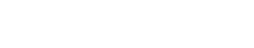
\includegraphics[width=0.98\linewidth]{figures/02_deep_learning/feature_vis/l11.pdf}
				} \\
				\subfloat[Layer $21$: patterns.]{
					\includegraphics[width=0.98\linewidth]{figures/02_deep_learning/feature_vis/l21.pdf}
				} \\
				\subfloat[Layer $31$: parts.]{
					\includegraphics[width=0.98\linewidth]{figures/02_deep_learning/feature_vis/l31.pdf}
				} \\			
				\subfloat[Layer $41$: structures.]{
					\includegraphics[width=0.98\linewidth]{figures/02_deep_learning/feature_vis/l41.pdf}
				}
				\caption[Feature visualizations from VGG16 layers]{Feature visualizations from VGG16 layers.}
				\label{fig:feature_vis_layers}
			\end{figure}
			
			\begin{figure}[!ht]
				\centering
				\subfloat[Scorpion]{
					\includegraphics[width=0.30\linewidth]{figures/02_deep_learning/feature_vis/classes_01_scorpion.png}
				}
				\subfloat[Tarantula]{
					\includegraphics[width=0.30\linewidth]{figures/02_deep_learning/feature_vis/classes_02_tarantula.png}
				}
				\subfloat[Centipede]{
					\includegraphics[width=0.30\linewidth]{figures/02_deep_learning/feature_vis/classes_03_centipede.png}
				} \\
				
				\subfloat[Seaslug]{
					\includegraphics[width=0.30\linewidth]{figures/02_deep_learning/feature_vis/classes_11_seaslug.png}
				}
				\subfloat[Crab]{
					\includegraphics[width=0.30\linewidth]{figures/02_deep_learning/feature_vis/classes_12_crab.png}
				}
				\subfloat[Stork]{
					\includegraphics[width=0.30\linewidth]{figures/02_deep_learning/feature_vis/classes_13_stork.png}
				} \\
				
				\subfloat[Unicycle]{
					\includegraphics[width=0.30\linewidth]{figures/02_deep_learning/feature_vis/classes_21_unicycle.png}
				}
				\subfloat[Violin]{
					\includegraphics[width=0.30\linewidth]{figures/02_deep_learning/feature_vis/classes_22_violin.png}
				}
				\subfloat[Wallclock]{
					\includegraphics[width=0.30\linewidth]{figures/02_deep_learning/feature_vis/classes_23_wallclock.png}
				}	
				\caption[Class visualizations from VGG16]{Visualization of classes learned by VGG16.}
				\label{fig:feature_vis_classes}
			\end{figure}
	
	\section{Deep Learning in Mobile Networks}
	
		% Rolf Stadler papers
		
		% Online feature selection
		% https://ieeexplore.ieee.org/abstract/document/9269066
		% https://arxiv.org/pdf/2112.08253.pdf
		
		% Service metrics
		% - Prediction distributions - https://ieeexplore.ieee.org/abstract/document/8584941
		% - Efficient learning on high dimensional data - https://ieeexplore.ieee.org/abstract/document/9012741
		% - Conditional density estimation - https://ieeexplore.ieee.org/abstract/document/9422765
		
		% Security strategies through reinforcement learning
		% https://ieeexplore.ieee.org/abstract/document/9269092
		
		% Online learning under resource constraints
		% https://ieeexplore.ieee.org/abstract/document/9464066
	
		\subsection{State-of-the-art}
			\label{cha:deep_learning:sec:related_work}
			
			Using the so far collected understanding of how deep learning and deep neural nets work and how they should be used, we can now take a critical look at how deep learning is utilized in mobile networks.
			\ac{5G} is the first mobile network generation that is meant to depend on advanced \ac{ML} techniques.
			In \ac{5G},	deep learning is regarded as both the solution to overcome the exponentially increasing complexity, and the enabler for many of the use cases previously thought to be impossible.
			\ac{5G} is already under development for some years now, so naturally, quite a volume of literature is available on deep learning in \ac{5G} networks.
			The different areas where \ac{DL} could be utilized are well summarized \cite{dl_mobile_survey}, also depicted in Fig.~\ref{fig:dl_mobile_uses}, and advanced use cases are detailed in \cite{can_book}.
			Some areas fall outside the boundaries of network automation: these are either low-level, real-time tasks (such as signal processing), or application-level tasks (such as application-level data analysis, or deep-learning-based applications).
			
			\begin{figure}[ht]
				\centering
				\includegraphics[width=\linewidth]{figures/02_deep_learning/dl_mobile_uses/dl_mobile_uses.png}
				\caption[DL topics in network automation]{Overview of topics in network automation utilizing deep learning \cite{dl_mobile_survey}.}
				\label{fig:dl_mobile_uses}
			\end{figure}
			
			The categories that fit the scope of (cognitive) network automation are:			
			\begin{itemize}
				\item \textbf{Learning Driven Network-Level Mobile Data Analysis:}
				Use cases here include traffic classification or \ac{QoE} from related, easily measurable \ac{QoS} \acp{KPI}.
				Another example is cell anomaly detection; detection of hardware or software faults, or misconfigurations using \acp{KPI} describing per-cell behavior.
				Yet another use case in this category is the long-term prediction of traffic or user growth, aiding network planning by predicting long-term demand.
				
				\item \textbf{Deep Learning Driven User Localization:}
				These use case cover the precise estimation of the user position using various localization techniques, to support location-based functionality, such as \ac{MDT} or mobility analysis.
				
				\item \textbf{Deep Learning Driven Mobility Analysis:}
				These use cases use the prediction of individual, or large crowd movement through wireless networks, for load balancing or predictive handover triggers in availability-critical services, such as \ac{URLLC}.
				
				\item \textbf{Deep Learning Driven Network Control:}
				Use cases here include dynamic resource allocation tasks, such as \ac{RRC}, routing or scheduling.
				An example of a resource allocation task is predictive network slicing, allocating multiple types of resources to services or users in the network.
				
				\item \textbf{Deep Learning Driven Network Security:}
				Use cases such as the detection of traffic anomalies, which can signal man-in-the-middle attacks, botnets or other security risks in the network.
			\end{itemize}		
			\noindent These categories all could utilize \ac{DL} in order to make decisions or to extract insight from a large variety and volume of data.
			However, not all of these possible \ac{DL} landing zones are actually considered, or do not utilize \ac{DL} to its fullest capabilities, as we will see shortly.
			
			% ------------------------------------------------------------------------------------------------------------------------------------------------------------------
			% Surveys + Summaries
			% ------------------------------------------------------------------------------------------------------------------------------------------------------------------
			
			% * AI for 5G: research directions and paradigms
			% * Intelligent 5G: When Cellular Networks Meet Artificial Intelligence
			% * Artificial Intelligence in 5G Technology: A Survey		
			
			% * Deep learning at the physical layer: System challenges and applications to 5G and beyond
			% * Deep learning for physical-layer 5G wireless techniques: Opportunities, challenges and solutions
			
			Different \ac{ML} techniques are often (incorrectly) referred to under the umbrella term \ac{AI} in mobile networks literature.
			The list of \ac{ML} algorithms that span the \ac{AI} ``spectrum'' is quite wide: complexity can range from simple statistical algorithms, such as linear regression, all the way to deep reinforcement learning algorithms using \acp{DQN}.
			This ``overselling'' is a constant problem in mobile network literature, which makes it hard to judge the actual capabilities of the utilized \ac{ML} algorithms at first glance, especially in surveys exploring the use of \ac{AI} in mobile networks.
			Most surveys recognize at least the $3$ main \ac{ML} principles, and refer to the following \ac{ML} algorithms in each principle \cite{ai_for_5g, ai_in_5g, intelligent_5g}:
			\begin{enumerate}[label=\textbf{\alph*})]
				\item \textbf{Supervised learning:}
				Supervised learning is the most commonly discussed \ac{ML} principle in surveys, and also contains the most complex learning algorithms.
				\ac{ML} algorithms that are utilized here include \ac{LR}, \acp{SVM}, \acp{HMM}, decision trees, and neural nets (the depth of which will be discussed shortly).
				Supervised learning is thought to be useful in tasks in all levels of the network, from root-cause analysis in network management all the way to channel estimation close to the physical layer.		
				This category usually also includes prediction tasks, which I don't consider as supervised-learning-based on the lack of human input needed for training data preparation (Sec.~\ref{cha:intro:sec:cognitive_cap_dl}).
				
				\item \textbf{Unsupervised learning:}
				Unsupervised learning is the least discussed principle in literature.
				The algorithms utilized here are often quite simple statistical methods, such as \ac{PCA}, \kmeans{}, \acp{GMM}, hierarchical and spectral clustering.
				More complex, but not deep learning capable algorithms include single class \acp{SVM} and \acp{SOM}.
				Deep learning capable neural nets, such as \acp{LSTM} are only discussed in the context of prediction, with the caveat of a strongly restricted model complexity because of the need for a short inference time in low-level tasks.
				Typically, unsupervised learning in higher-level (management) tasks are considered only to support the generation of labeled training datasets for later supervised learning algorithms, which actually implement the management functionality \cite{ai_for_5g}.
				
				\item \textbf{Reinforcement learning:}
				Reinforcement learning is an often discussed tool in the context of optimization tasks, such as resource allocation or self-configuration, or even in high-level management or network planning tasks.
				The reinforcement learning principle by nature requires quite complex algorithms, which range from the more traditional Q-learning to recent \acp{DQN}, often utilizing deep neural nets such as \acp{LSTM}.
			\end{enumerate}	
		
			% Individual papers		
			% ------------------------------------------------------------------------------------------------------------------------------------------------------------------
			% Organizing per topic
			% ------------------------------------------------------------------------------------------------------------------------------------------------------------------
			
			% Short-timeframe radio interface control
			% * Deep learning-based mmWave beam selection for 5G NR/6G with sub-6 GHz channel information: Algorithms and prototype validation - Beam selection  - Supervised Classification (Deep FC net)
			% * Deep learning based pilot allocation scheme (DL-PAS) for 5G massive MIMO system - Short timeframe MIMO/Beam control - Supervised Classification (Shallow FC) 
			% * A deep-learning-based radio resource assignment technique for 5G ultra dense networks - Short timeframe RRC - ? Prediction (Shallow LSTM)
			% * Deep learning for radio resource allocation with diverse quality-of-service requirements in 5g - Short timeframe RRC - Supervised Regression (Two Shallow FC nets)
			% * Channel state information prediction for 5G wireless communications: A deep learning approach - Channel quality prediction - Short-timeframe Sequence Prediction (Quite deep CNN + LSTM)
			% * Performance Evaluation of Channel Decoding with Deep Neural Networks - Channel decoding - Supervised regression (shallow MLP, CNN and RNN, authors say restrictive)
			
			% High-level resource allocation
			% * Deep reinforcement learning for dynamic computation offloading and resource allocation in cache-assisted mobile edge computing systems - MEC offloading and cache allocation w/ reinforcement learning - DQN
			% * Intelligent Offloading in Multi-Access Edge Computing: A State-of-the-Art Review and Framework - Placement in MEC - DQN
			% * A deep reinforcement learning based framework for power-efficient resource allocation in cloud RANs - Cloud RAN resource allocation - DQN
			% 
			% * DeepCog: Cognitive network management in sliced 5G networks with deep learning - Slicing - Supervised Prediction (Medium Deep 3D CNN + FC)
			% * Deep Reinforcement Learning for Resource Management in Network Slicing - Network Slicing resource allocation - DQN		
			% * Deepslice: A deep learning approach towards an efficient and reliable network slicing in 5G networks - Network slice prediction - Fancy Classification (which slice it should be assigned) (Shallow FC net)
			
			% Traffic anomaly detection
			% * A self-adaptive deep learning-based system for anomaly detection in 5G networks - Traffic anomaly detection (security) - Supervised Classification (Shallow FC (DBN, SAE)) 
			% * An efficient deep learning model for intrusion classification and prediction in 5G and IoT networks - Traffic anomaly detection (security)  - AE pretraining + Supervised Classification (AE ?, classifier shallow FC net)
			% * Deep Learning-Based Big Data-Assisted Anomaly Detection in Cellular Networks - Sleeping cells finally - Supervised classification (Quite deep MLP)
			
			% Outlier:
			% * Deep learning for hybrid 5G services in mobile edge computing systems: Learn from a digital twin - User association w/ digital twin (mobility, association, offloading) - Prediction (lables w/ twin) (Shallow-medium FC net)
			
			The above referenced surveys discuss a quite broad range of algorithms with varying complexity, and in my opinion provide an unfocused view of what constitutes today as deep learning in mobile networks.
			In order to get a representative, unbiased view of what is currently discussed as deep learning in \ac{5G}, I conducted my own survey by searching for papers which include the ``\ac{5G}'' and ``deep learning'' keywords on IEEEXplore\footnote{\url{https://ieeexplore.ieee.org/}}.
			The below papers were gathered by sorting the results from the query by the decreasing number of citations.
			I manually selected papers which are a) on the topic of mobile network operation on all levels (but not applications in mobile networks which use \ac{DL}) and b) reasonably recent.
			I found that most of the papers can be organized into $3$ use case groups:
			\begin{enumerate}[label=\textbf{\alph*})]
				\item 
					\textbf{Short-timeframe radio interface control:}
					These tasks involve the reconfiguration of the radio interface such as \ac{MIMO} control or beam selection \cite{dl_based_beam_select, dl_based_pilot_alloc}, \ac{RRC} \cite{dl_based_rrc, dl_for_rrc}, the prediction of channel quality \cite{channel_state_pred} or even the task of channel decoding itself \cite{channel_decoding_dl}.
					These tasks require frequent inference cycles, often close to per \ac{TTI} ($10$s of milliseconds), while in even more extreme cases, such as channel decoding, latency budgets for inference are as small as only a few microseconds \cite{dl_phys_survey}.
					A further constraint is the limited computational capacity available in mobile devices, as well as the need to conserve battery life with lightweight algorithms.
					All these constraints limit the allowed complexity of the \ac{DL} algorithms used close to the physical layer, which for neural nets means the limitation of layer widths and the number of layers in order to reduce the number of weights/parameters in the net \cite{dl_phys_survey2}.
					Most of them use shallow \ac{FC} or convolutional nets, or simple \acp{LSTM}, which limits the ``deep'' learning capacity of these nets by reducing the number of hierarchical features to be possibly learned.
					The majority of these works use some form of supervised learning, such as classification, or regression to a predefined function found by convex optimization or exhaustive search.
				
				\item
					\textbf{High-level resource allocation:}
					A large portion of these works involve the resource allocation in cloud environments, such as intelligently caching or offloading applications in \ac{MEC} \cite{mec_offload_cache, mec_offload}, or resource allocation in cloud-\ac{RAN} \cite{cloud_ran_resource}.
					These tasks are frequently solved with reinforcement learning, often utilizing \acp{DQN} to learn and optimize a resource allocation strategy in a simulated environment.
					Other, even more complex vertical resource allocation tasks involve network slicing, where both physical and virtual resources are allocated end-to-end in the network for user types or applications \cite{slicing_resource, drl_slicing_resource, slicing_resource2}.
					Network slicing papers often use classification as an \ac{ML} principle, as well as reinforcement learning, in both of which the nets used can be quite deep and thus realize deep learning.
							
				\item
					\textbf{Traffic anomaly detection:}
					This area is involved in the detection of anomalous traffic patterns in the network, which could stem from malicious attacks such as botnets \cite{anomaly_botnet}, intrusions over radio \cite{anomaly_intrusion}, or software or hardware failures \cite{anomaly_sleeping}.
					Although anomaly detection could be undertaken with unsupervised algorithms, by modeling normal behavior and detecting patterns that fall outside of this model, most of the current works use supervised learning algorithms.
					With supervised learning and the correct dataset, generally, a higher precision can be achieved with much simpler models, which is also represented in the quite shallow \ac{FC} nets used by these works.
					Unfortunately, this also limits the capability of these nets to learn hierarchical features, thus not really realizing deep learning.		
			\end{enumerate}
		
			Many of the listed works utilize shallow, simple neural nets, which would not be necessarily considered as deep-learning-capable.
			This is especially true in low-level tasks close to the physical layer, where inference execution time is limited.
			High-level, large-scale or management-oriented tasks don't suffer from these timing constraints, thus the possibility to employ \ac{DL} is greater here.
			However, often in these tasks the amount of data needed to truly utilize the capabilities of \ac{DL} is overwhelming, and is not yet supported or produced by current mobile networks, thus researchers tend to fall back to simpler \ac{ML} models.
			Workarounds to this problem exist, such as the utilization of complex digital twins to produce training data for these high-level tasks \cite{dl_digital_twin}, but this usually requires extraordinary effort for many tasks and is simply not available for most researchers.			
			
			My takeaway is that deep learning is too often used only as a buzzword in \ac{5G}-related papers: while I don't doubt the possible benefits of using \ac{DL} for the above tasks, I question whether the employed \ac{ML} algorithms are truly capable of deep learning.
			Furthermore, in places where complex unsupervised \ac{DL} algorithms could provide the benefit of robustness or adaptability, instead simpler, supervised algorithms are used to achieve a small accuracy gain of a few percentage points.
			I think investigating unsupervised deep learning in many of these tasks could be worthwhile and provide a benefit over current solutions, or allow for new use cases.			

		\subsection{Drivers, Enablers and Constraints of DL}
			\label{cha:deep_learning:sec:constraints}
			
			The capability of deep neural nets comes at cost: with great cognitive power come great computational requirements.
			For deep neural nets, the drivers and constraints are intertwined, creating a complex landscape through which one must navigate when aiming to develop these algorithms.
			
			\subsubsection*{Computational power}
			
				As the basic steps to train neural nets through backpropagation and gradient descent are very atomic algebraic tasks, there is little room to algorithmically optimize these calculations.
				However, as these tasks are highly parallelizable, there are significant opportunities to speed up the computation through implementations using hardware capable of massively parallel computations.
				This has created a two-step cycle of progression for \acp{DNN}:
				\begin{enumerate}[label=\textbf{\alph*})]
					\item Neural nets are improved, allowing for deeper, more complex topologies to be trained but with major increases in computational requirements.
					\item Hardware capabilities and storage capacity is improved, allowing for the complex \acp{DNN} to be trained and tested in humanly acceptable timeframes, e.g., purpose-built hardware and new implementations emerge to further speed up computations.				
				\end{enumerate}
				\noindent Nowadays, all but the simplest neural nets require dedicated hardware -- usually in the form of \acp{GPU} -- to train and infer within a reasonable time.
				These \acp{GPU} are slowly becoming more and more widespread both in end-user devices (mobile phones), and in the network itself (edge clouds).
				However, running the inference on either side is problematic: mobile phones have a limited battery life, and should conserve it by minimizing \ac{DL} computation.
				This can be achieved by offloading computation to the edge cloud, but in this, case the amount of data communicated can be overwhelming, or security and privacy concerns can emerge if the user's data is sensitive.
			
			\subsubsection*{Timing constraints}
			
				Current improvements sometimes achieve only a few $1/10$ of a percent increase in accuracy at the cost of a $10$-fold increase in training and inference time.
				However, these seemingly small increments in accuracy amount to a large forward-step in cognitional power need, which in turn means a significant increase in processing time.
				Deep neural nets can have two types of constraints for processing time:
				\begin{enumerate}[label=\textbf{\alph*})]
					\item A hard time-limit at inference, so that the net is able to process the constant stream of information at the rate it is arriving, such as the case with object recognition in video processing.
					\item A softer time-limit at training, so that the neural net can be trained in a reasonable timeframe.
				\end{enumerate}	
				\noindent The time it takes to develop a concept into prototype -- mainly influenced by the models’ training time -- is critical in deep learning research.
				Although most common architectures nowadays can be trained on desktop computers, the need for speed and simplicity implies that buying expensive, specialized hardware dedicated to deep learning is not a waste.
				This is the reason why the leading institutions in the field utilize huge supercomputers; being able to validate a concept quickly without spending much effort on optimization is invaluable in the deep learning race.
			
			\subsubsection*{Quantity of data}
			
				The companies most invested in deep learning are those that handle large amounts of data, usually in the form of images, videos, or text, where the automation of tasks previously solved by humans would mean a huge decrease in cost and a large increase in capacity.
				This large amount of information, however, is not only a burden; the quantity and quality of available data is what enables the training of the learning machines more than any hardware or algorithmic improvement could.
				Within this lies a big problem for \ac{DL} in mobile networks: mobile network vendors -- the ones potentially developing the \ac{DL} algorithms -- are cut off from the source of the data, the large-scale mobile network deployments, as these are owned and run by network operators.
				Sharing data from network operators requires agreements on both sides, good cooperation and a lot of effort in order to maintain anonymity for the users, or avoid leaking sensitive information about the operator itself.
				This effort is seldom profitable for the operator, thus, they are usually reluctant to share data, leaving the vendors without access to the fundamental enabler of \ac{DL}.
					
			The consideration of these aspects of \ac{DL} is crucial when developing algorithms.
			Many good ideas on paper turn out to be problematic in one of the above topics, when a real deployment is considered in a mobile network.
			This is the reason why my research objectives include such considerations, and why these topics are going to be further discussed throughout this thesis.			
			

	
	\part{Exemplification}
		\label{part:exemplification}
		\chapter{Quantization for Network State Modeling}
	\label{cha:quantization}
	
	When communicating with others, we often use the description of a single entity to describe the characteristics of a whole group.
	Using examples in this form is a very effective way of conveying information; the listener intuitively understands that the highlighted aspects are what distinguish the given group from the rest, while also keeping in mind that there are likely entities in the group with slightly differing attributes compared to the example given.
	Using examples are most important when describing a large amount of entities, in which case multiple examples are usually given to cover the whole range of attributes.
	However, selecting which examples to use in order to maximize their descriptiveness can be quite a challenge.
	
	\emphix{Quantization}{quantization} realizes this task as a \ac{ML} algorithm, in which a large number of observations with a continuous distribution (the dataset) are mapped to a small set of discrete observations (the examples/prototypes/centroids).
	Quantization algorithms split the input space into a finite number of partitions, and use a single observation from within each partition as an exemplary representation of all the observations in that partition.
	Just as in human communication, exemplification through quantization also serves the purpose of effective communication for machines, by maximizing the amount of useful information communicated with a minimum amount of data.
	Quantization algorithms are primarily used in signal processing, where their task is to remove minute variance from the data, and compress the information into the smallest possible encoding, which can then, e.g., be transmitted over radio, or effectively stored on a hard drive.
	
	Quantization is not to be confused with clustering; while in clustering, the goal is to find originally present groups in the data, quantization only aims to partition the data into possibly arbitrary parts, in order to effectively compress information.
	Quanta do not necessarily adhere/align to clusters in the data, because in most use cases, the quantization will use far more quanta than the number of groups present.
	However, as we will see later, good quantization algorithms do have to take into consideration clusters in the data, thus blurring the division between clustering and quantization algorithms.
	
	Communication through examples is also useful in network automation, where the quanta can be seen as \emphix{network states}{network state}, which describe the settings, current performance, and/or context of single or multiple entities in the network, such as base-stations, gateways, cells, or even users.
	Network states are meant to form the basis of communication -- a vocabulary -- between cognitive functions in the mobile network, upon which control decisions or reconfiguration requests can be based.
	Because the mobile network is understood to be a dynamically changing context, it is important to have the network states automatically defined, so that in case of a context change, they can be quickly redefined without human supervision, making the management system adaptive to change.
	
	Sec.~\ref{cha:quantization:sec:knowledge_sharing} introduces the concept of knowledge sharing for self-healing -- which uses quantization and some form of network states -- through the following patent application:
	
	\begin{patent}
		Diagnosis Knowledge Sharing for Self-healing \\
		\textit{Benedek Schultz, Janne Ali-Tolppa, Márton Kajó} \\
		WO, PCT application no.: PCT/EP2018/079735, filed Oktober 2018
	\end{patent}

	Sec.~\ref{cha:quantization:sec:bvq} of this chapter is based on the work published in the following paper:
	
	\begin{publication}
		Equal-volume Quantization of Mobile Network Data using Bounding Spheres and Boxes \\
		\textit{Márton Kajó, Benedek Schultz, Janne Ali-Tolppa, Georg Carle} \\
		NOMS 2018-2018 IEEE/IFIP Network Operations and Management Symposium, pp. 1-9. IEEE, 2018.
	\end{publication}
	
	My contributions to the above paper was the design, implementation and evaluation of the algorithm, as well as the co-authoring of the paper.
	The discussion in this thesis expands on the paper, by placing it into the larger concept of knowledge sharing in self-healing, as well as the proposal of an alternative, neural-net-based implementation, published in the following report (Sec.~\ref{cha:quantization:sec:nn_quant}):
	
	\begin{publication}
		Neural Network-based Quantization for Network Automation \\
		\textit{Márton Kajó, Stephen S. Mwanje, Benedek Schultz, Georg Carle} \\
		arXiv preprint arXiv:2103.04764 (2021).
	\end{publication}

	My contribution to this technical report was the design, implementation and evaluation of the algorithm, as well as the authoring of the document itself.
	While containing important details for our future work, we deemed the content of this report to be too technical for a mobile-networks-oriented audience (please see Sec.~\ref{cha:conclusion:sec:dl_research} for further notes on this), thus, instead of publishing it as a scientific paper, the report was made freely available on arXiv.
	
	The overall discussion is concluded with some remarks on the complexities of implementing algorithms for massive parallelization, and integrating them into \ac{DL} frameworks or algorithmic pipelines, a topic which came up often in our research.

	Some of the findings from this work as are also echoed in the following publications (both of which I also co-authored, but no additional text is used from them in this dissertation):
	
	\begin{publication}
		Self-healing and Resilience in Future 5G Cognitive Autonomous Networks \\
		\textit{Janne Ali-Tolppa, Szilárd Kocsis, Benedek Schultz, Levente Bodrog, Márton Kajó} \\
		2018 ITU Kaleidoscope: Machine Learning for a 5G Future (ITU K), pp. 1-8. IEEE, 2018.
	\end{publication}

	\begin{publication}
		Cognitive Autonomy for Network Self‐Healing \\
		\textit{Janne Ali-Tolppa, Márton Kajó Georg, Borislava Gajic, Ilaria Malanchini, Benedek Schultz, Qi Liao} \\
		Towards Cognitive Autonomous Networks: Network Management Automation for 5G and Beyond (2020): 345-384.
	\end{publication}

	\section{Concept: Diagnosis Knowledge Sharing for Self-Healing}
		\label{cha:quantization:sec:knowledge_sharing}
		
		\subsection{Automating Diagnosis in Self-Healing}
			
			Network assurance relies largely on monitoring the alarms generated by network elements, or by monitoring their performance directly.
			Alarms are triggered through the process of \ac{FM}, where individual network elements monitor preset thresholds, and generate alarm messages if a threshold is overstepped.
			The diagnosis of discovered anomalies often relies solely on human inference.
			Given the complexity and growth of mobile networks, such processes do not scale, and will become infeasible in the near future.
			Consequently, there is a need for augmented processes in relation to networks for diagnosing network anomalies.
			In this context, augmented refers to processes where human inference is supplemented by \ac{ML}, in order to reduce labor and speed up processing, hopefully ultimately leading to full automation.
			At the time of this work, we had solutions for automated anomaly detection, but not for augmented or automated diagnosis.
			
			One of the main focuses of \ac{SON} is self-healing, where the goal is to automatically detect and correct faults in the network.
			The self-healing process can be split up into $3$ steps: the detection, diagnosis, and correction of faults.
			The deployment of corrective actions is a quite complicated topic, and has been researched extensively \cite{tsvetko_verif_1, tsvetko_verif_2}, thus it will not be discussed here, instead, this work focuses on the preceding step, the diagnosis of anomalies, for which the detection process has to be introduced.
			
			The detection of anomalies can be automated in a conceptually straightforward way \cite{anonamly_det}, by comparing the current performance to an established profile that describes the normal behavior of the network.
			These profiles are likely formed by \ac{ML} algorithms, such as neural nets.
			The profiles are created from \ac{PM} measurements of a set period, and can be updated either periodically or continuously to combat profile aging, thus creating resilience against false detections stemming from slow, trend-like changes in network behavior.
			The profiling and detection are done based on a set of selected features, e.g. \ac{PM} \acp{KPI}, the composition of which depends on the types of problems that are to be detected.
			Such a detection method can be done on the network management level, where a wider overview of the network is available, and detected anomaly events can be correlated over the whole network.
			While \ac{FM} alarms cover many of the recognized network faults, \ac{ML}-based anomaly detection methods can profile and learn the normal behavior for each context, e.g. for each network function, and possibly detect previously unseen deviations from it.
			Such a function enables a more sensitive detection system, which works by correlating information from multiple layers or elements in the network.
			This makes the system able to recognize issues where no explicit alarm is generated, or detect anomalies before an alarm is raised and a severe problem occurs.
			
			\begin{figure}[ht]
				\centering
				\includegraphics[width=0.4\linewidth]{figures/03_quantization/anomaly_pattern/anomaly_pattern.png}
				\caption[Anomaly pattern examples]{An example of an anomaly pattern (red) compared against the best match (blue) in the diagnosis knowledge base, depicted on a radar-chart.}
				\label{fig:anomaly_pattern}
			\end{figure}
			
			An anomaly detection function defines distinct \textbf{anomaly events} both temporally and spatially, by specifying the timeframe and the affected network elements of the anomaly.
			Using a larger scope of collected \ac{PM} measurements during the anomaly event, \textbf{anomaly patterns} are formed which describe the characteristics of the anomaly.
			The anomaly pattern can consist of a vector of the normalized anomaly levels of each \ac{KPI} in a cell or multiple cells, or the raw \ac{KPI} values during the anomaly.
			Often these values are aggregated over time in the anomaly pattern.		 	
			After an anomaly is detected and an anomaly pattern is established, a diagnosis component analyses the anomaly pattern and tries to determine its root cause.
					
			Like other semi-automated implementations of self-healing topics, diagnosis rules are often defined a-priori by an expert.
			This static rule-based diagnosis knowledge base goes against our goals of a fully-automated self-healing system.
			An alternative, which allows a more dynamic, automated collection and maintenance of the diagnosis knowledge base is to use \ac{CBR}, where the diagnosis of an anomaly event is done by automated generalization and extrapolation from previous, similar examples of anomalies.
			However, for \ac{CBR}-type diagnosis to work, preferably a large database of previously diagnosed anomalies would need to be maintained.
		
			Automated diagnosis is a complicated task, largely due to the less-constrained problem formulation, accentuated by the distributed and heterogeneous nature of mobile networks.
			As diverse as fault states can be, they occur only in very rare cases, which makes it near impossible to collect statistically meaningful data for each case.
			The lack of a statistically relevant amount of samples makes the reliable root-cause analysis extremely difficult, especially so when utilizing \ac{DL}, which mainly relies on plentiful training observations for a correct model formulation (see Sec.~\ref{cha:deep_learning:sec:overfitting}).
			Thus, it is of utmost importance that diagnosis information is collected and reused from every possible source, by sharing it between different contexts, such as different network deployments or timeframes, software versions, or other discontinuities that could otherwise invalidate the already learned models.
			
			The manual collection and maintenance of such a shared diagnosis knowledge base would be tedious and expensive at best.
			Therefore, automated knowledge sharing of insights is required to achieve a maintainable diagnosis system for self-healing.
			This would be especially important in cases, where new network functions are introduced in the network, or even completely new networks are deployed.
			Such cases where models are learned in one task and context, and are applied to another task or context, is called transfer learning.
			Typically, transfer learning is hard to achieve, and is currently one of the leading topics of research in machine learning.
		
		\subsection{Knowledge Sharing using Quantization}
		
			The goal of a diagnosis knowledge sharing process between autonomous and cognitive diagnosis functions in different contexts (e.g. in different network instances), is to be able to share insights in a way well-suited for \ac{CBR}-type diagnosis functions, and incrementally improve the diagnosis capabilities of each other.
			The scenario we discuss here is one where multiple \acp{LDA} are connected to a single \ac{CDA} (Fig.~\ref{fig:diag_lda_cda}).
			The \acp{LDA} manage local, context-specific diagnosis knowledge bases, which contain previously diagnosed anomaly patterns with their diagnosis attached as a label.
			The central \ac{CDA}'s goal is to collect, harmonize and retain a large base of diagnoses which contains the most prevalent anomaly patterns from all previously seen contexts.
			
			\begin{figure}[ht]
				\centering
				\includegraphics[width=0.8\linewidth]{figures/03_quantization/diag_lda_cda/diag_lda_cda.pdf}
				\caption[CBR diagnosis with knowledge sharing]{CBR diagnosis process with knowledge sharing.}
				\label{fig:diag_lda_cda}
			\end{figure}
			
			Both the local and central knowledge bases are updated either by a human expert, or a \ac{CBR}-type automated diagnosis function in case a new anomaly pattern is introduced.
			However, in order to realize knowledge sharing, the \acp{LDA} and the \ac{CDA} are connected through a \textit{knowledge sharing interface}.
			The communication on this knowledge sharing interface is imagined through the use of some form of vector quantization.
			
			The information communicated between the agents can be seen as a request for help in refining/extending their respective models.
			The information going in both directions is made up of labeled quanta, and optionally a collection of specific anomaly instances for which the respective agent decided that they do not fit its subjective model well.			
			Most quantization algorithms expect their input as a set of points, with a usual option of defining a starting position for the quantum centroid.
			However, here the quantization algorithms need to be able to run on an input comprised of a mix of clusters and outlying points.
			This functionality can be synthesized if individual points are sampled from a local database to recreate the distribution of points contained in the given clusters.
			If individual points were also communicated, these can be mixed to the synthesized points.
			Using this semi-synthetic set, the quantization algorithm can start from the locally saved previous state, and run until convergence.
			An example of the whole procedure can be seen in Fig.~\ref{fig:diag_knowledge_sharing}.			
			The (re-)sampling procedure allows the \ac{CDA} to maintain a diagnosis database of a constant size, rather than continuously collecting information.
			
			\begin{figure}[ht]
				\centering
				\subfloat[Input information]{
					\includegraphics[width=0.4\linewidth]{figures/03_quantization/diag_knowledge_sharing/diag_knowledge_sharing_1.pdf}
				}
				\subfloat[Sampling and mixing]{
					\includegraphics[width=0.4\linewidth]{figures/03_quantization/diag_knowledge_sharing/diag_knowledge_sharing_2.pdf}
				} \\
				\subfloat[Local model starting position]{
					\includegraphics[width=0.4\linewidth]{figures/03_quantization/diag_knowledge_sharing/diag_knowledge_sharing_3.pdf}
				}
				\subfloat[fitting]{
					\includegraphics[width=0.4\linewidth]{figures/03_quantization/diag_knowledge_sharing/diag_knowledge_sharing_4.pdf}
				}
				\caption[Diagnosis knowledge sharing]{Quantization procedure incorporating local starting positions and mixed input information.}
				\label{fig:diag_knowledge_sharing}
			\end{figure}
			
			The quantization serves two purposes: firstly, it is a fine enough discretization of the anomaly pattern space, with which the different anomaly’s root causes can be described by attaching a single diagnosis/root cause to each of the quanta.
			Secondly, the quanta also serve to describe the anomaly event distribution in the anomaly pattern space, from which the original statistical distribution can be reconstructed/resampled with enough precision.			
			In the bigger picture, the described method transfers knowledge or new information from a source model to a target.
			This is true regardless of the source being the \ac{LDA} and the target being the \ac{CDA}, or vice-versa.
		
%		\subsection{Quantum Splitting and Merging}	
%			
%			To be able to automatically fit the model complexity to the complexity of the underlying data structure, quanta need to be dynamically added or removed from the model.
%			Automatic decisions can be implemented to decide when to split or merge quanta based on some form of goodness-of-fit value, which creates a measure of confidence in the model.
%			Model confidence should be higher if the goodness-of-fit increases, or if the model complexity decreases.
%			
%			\begin{figure}[ht]
%				\centering
%				\subfloat{
%					\includegraphics[width=0.4\linewidth]{figures/03_quantization/diag_split_merge/diag_split_1.pdf}
%				}
%				\subfloat{
%					\includegraphics[width=0.4\linewidth]{figures/03_quantization/diag_split_merge/diag_split_2.pdf}
%				}
%				\caption{Quantum splitting.}
%				\label{fig:diag_split}
%			\end{figure}
%			
%			Splitting is done in case many points are lying outside a quantum, where an additional quantum could cover the outlying points so well that it counteracts the decrease in confidence stemming from the increased model complexity.
%			Split quanta should carry over labeling information within certain limits regarding distance from the original cluster, overlap of the clusters or surrounding clusters with the same/different labels.
%			If no labeling information can be assigned to the newly formed clusters with high confidence, clusters are left as unlabeled and the knowledge sharing process is started.
%			An example of cluster splitting can be seen in Fig.~\ref{fig:diag_split}.
%			
%			\begin{figure}[ht]
%				\centering
%				\subfloat{
%					\includegraphics[width=0.4\linewidth]{figures/03_quantization/diag_split_merge/diag_merge_1.pdf}
%				}
%				\subfloat{
%					\includegraphics[width=0.4\linewidth]{figures/03_quantization/diag_split_merge/diag_merge_2.pdf}
%				}
%				\caption{Quantum merging.}
%				\label{fig:diag_merge}
%			\end{figure}
%			
%			The merging of quanta follows the same basic concept as splitting.
%			Two quanta should be merged if the decrease in model complexity overtakes the potential increase in goodness-of-fit.
%			Labeling information can be carried over from the original quanta if it fulfills criteria regarding similarity of parent labels, surrounding labels, and overlap.
%			Otherwise, the newly formed quantum is unlabeled and the knowledge sharing process is started.
%			An example of quanta merging can be seen in Fig.~\ref{fig:diag_merge}.

		% ITT - READ END

		\subsection{Towards Equal-Volume Quantization}
		
			The diagnosis knowledge sharing concept was the first occurrence in our work, where some form of quantization was meant to be used as a basis for communication between cognitive functions.
			Several aspects in it influenced the design of the bounding volume quantization algorithms, which are the topic of the next section (Sec.~\ref{cha:quantization:sec:bvq}):
			\begin{itemize}
				\item 
					\textbf{Equal volumes}:
					The roughly equal volumes of the quanta are needed to be able to establish a uniform ``resolution'', with which the labeling process operates.
					While providing a very simple goodness-of-fit metric (maximum quantization error), this also helps in the easy definition of cluster merging and splitting criteria based on relative distance between points and quantum centroids, or between two quantum centroids.
				
				\item
					\textbf{Continuous learning}:
					The knowledge sharing concept is built around a quantization, where the fitting procedure can be continued at any time, even if the training points are completely replaced.
					The \ac{EM} iterative optimization framework makes this inherently possible, by simply continuing the iterations whenever further fitting is required.
				
				\item
					\textbf{Mixed inputs}:
					The quantization algorithm was meant to be capable of fitting a mixed set of predefined quanta and individual observations without the proposed resampling mechanism.
					Although we did not propose this modification neither in the paper, nor in the invention, such a functionality was planned in case the knowledge sharing concept was to be further pursued.					
			\end{itemize}
			
			The diagnosis knowledge sharing concept was, in my opinion, quite far in the development process, close to being evaluated on data from a real mobile network deployment.
			Unfortunately, this data would have originated from an operator, with which Nokia ultimately could not agree on data-sharing conditions.
			Given this larger dataset, the work detailed in the next section would have also contained the evaluation results from the knowledge sharing scenario.
			Ultimately, lacking this dataset meant that we had to use a simpler, smaller dataset, which lead to us using use cases such as visualization or anomaly detection.
			In the end, we were never able to source large-scale network data of the type needed for this evaluation, thus the diagnosis knowledge sharing concept is only discussed in the respective patent.
	
	\section{Density-Invariant Quantization with Bounding Volumes}
		\label{cha:quantization:sec:bvq}
	
		\subsection{Quantization in High-Dimensional Spaces}
			\label{cha:quantization:sec:high_dim_problem}		
			
			Most often, quantization is used to refer to basic numerical processes, such as rounding to the nearest integer.
			While technically a correct interpretation, rounding and other per-dimension quantization methods are not feasible if the input data is high-dimensional.
			To illustrate this lack of scaling with the dimensionality, let us imagine a simple unit rectangle, populated by a number of points, representing the observations in our training dataset.
			The simplest quantization in this rectangle is to split every dimension into $2$ partitions, arriving at $4$ bins into which the datapoints can fall.
			By increasing the number of dimensions to $3$, the same scheme gives us $8$ bins, and so on.
			The equation (Eq.~\ref{eq:bin_curse_of_dim}) that governs the number of bins can be seen in Fig.~\ref{fig:perdim_curse}, where $n_{bins}$ refers to the number of attained bins, $p$ is the number of partitions per-dimension, and $d$ is the number of dimensions.
				
			\begin{figure}[ht]
				\centering
				\begin{minipage}[t]{0.2\linewidth}
					\begin{equation}
						\label{eq:bin_curse_of_dim}
						n_{bins} = p^d,
					\end{equation}
				\end{minipage}
				\begin{minipage}[t]{0.6\linewidth}
					\raisebox{-0.8\height}{\includegraphics[width=\linewidth]{figures/03_quantization/perdim_quant/perdim_quant.pdf}}
				\end{minipage}
				\caption[Illustration of the curse of dimensionality in per-dimension quantization]{Illustration of the curse of dimensionality in per-dimension quantization.}
				\label{fig:perdim_curse}
			\end{figure}
			
			Increasing the dimensions further can quickly lead to a number of bins which is greater than the number of datapoints.
			This situation defeats the purpose of quantization; it is likely that some bins will be left unpopulated or contain only a few datapoints, while a few bins will contain the majority the datapoints.
			This situations means the quantization does not compress information effectively, or at all.
			It is easy to see that the exponential scaling of the number of bins with the number of dimensions can overcome any reasonably-sized dataset with even the lowest number of bins per dimension, thus, such quantization methods do not work with high-dimensional input data.
			This effect is just one aspect of the \emphix{curse of dimensionality}{curse of dimensionality} -- the behavior of high-dimensional spaces -- which will come up often in this thesis \cite{curse_of_dim}.
			
			Mobile network data exhibits the above described problem; in \acp{OSS}, thousands of \acp{KPI} are collected on a minutely basis, where \acp{KPI} function as separate dimensions, making up a high-dimensional space in which observations exist as individual datapoints.
			To achieve a sensible quantization in such spaces, instead of per-dimension quantization, vector quantization algorithms are used.
			These algorithms define a number of quanta in a way which is independent of the number of dimensions, freeing the quantization from the curse of dimensionality at least a little.
			Furthermore, the quanta ``stick'' to populated areas of space, so that every quanta is almost guaranteed to be populated (as long as $n_{quanta} \leq n_{datapoints}$).		
			
			In the following, multi-dimensional observations making up a dataset will are referred to as either datapoints, or just simply points.
			A set of points belonging to the same partition are referred to as a \emphix{quantum}{quantum}.
			A quantum \emphix{centroid}{centroid} is a single point -- a prototype -- that represents (the most important characteristics of) the whole quantum.
			The quantum centroid is neither necessarily the geometric center of the set of points, nor one of the points.
			The distance between a quantum centroid and an observation assigned to that quantum is the \emphix{quantization error}{quantization error} of that observation.
			The distance measure is the Euclidean distance (or squared distance, the $L_2$ metric) if not stated otherwise.
			If an area of the input space is sparsely populated (i.e.: contains few or no datapoints), it simply referred to as \emphix{sparse}{sparse space}, or \emphix{dense}{dense space} if the contrary is true.
			
			Vector quantization algorithms were originally conceived for the purpose of data compression.
			By replacing each observation with its closest quantum centroid, stored or transmitted information can be greatly compressed at the cost of losing the information contained within the quantization error vector.
			In the following, a (non-exhaustive) list of currently popular algorithms, and a brief description of their optimization targets is presented:
			\begin{itemize}
				\item 
					\textbf{\kmeans{}:} More precisely Lloyd's algorithm \cite{lloyd} was originally conceived as a signal quantization method.
					The \kmeans{} algorithm partitions the data into \textit{k} quanta so that the sum of quantization errors on all observations is minimal.
					This results in an accurate quantization of dense areas but a less precise quantization of sparse areas, for which a fewer number of quanta is assigned.
				
				\item 
					\textbf{Self-Organizing Maps, Neural Gases:} These algorithms follow the competitive learning paradigm, in which each quantum is competing with the others for a ``right to respond to a given subset of inputs'' \cite{complearn}.
					In this approach, areas that are sparsely populated present a smaller reward and draw fewer quanta, resulting in similar behavior to \kmeans{}.
				
				\item
					\textbf{Sparse Autoencoders:} Autoencoders show similar behavior to quantization methods if activation sparsity is enforced in the encoding; nodes in the hidden layers are assigned to (distinct) parts of the input space \cite{ksparse}.
					Activation sparsity refers to a different concept as previously introduced, and is discussed in more detail later in Sec.~\ref{cha:sparse_clust:sec:act_sparse}.
					Since autoencoders optimize data compression by minimizing the loss of overall information, this also translates to having fewer nodes assigned to sparsely populated areas in the input space, resulting in greater compression and greater quantization error in those areas.
			\end{itemize}
			\noindent Although the optimization targets of the approaches presented above are different, they result in similar behavior: sparse areas of the input space are mapped with less precision, quanta assigned to these have a greater maximum quantization error.
			
			In many applications, sparse areas of the data are just as important -- or even more important -- as dense areas.
			In these cases, the representation of densely and sparsely populated areas with at least the same precision is desired.
			Thus, instead of minimizing the sum of quantization errors, we propose that it is better to strive for the minimization of the maximum quantization error in these cases.
			Tightly fitting a bounding shape, such as a sphere, to wrap the points in a quantum allows us to define an assigned volume of the quantum.
			The bounding shape's exact position and size is only governed by the points farthest from the quantum center; in this regard, the points with the largest quantization error are effectively setting the assigned volume of the quantum they are in.
			Equal and minimal maximum quantization error between quanta can be achieved by the equalization of this assigned volume, which is the main idea presented in this section.
		
		\subsection{Uses of Equal-Volume Quantization in Mobile Networks}
			\label{cha:quantization:sec:equal_probelm}
			
			Mobile network \ac{PM} data often contains a wide variety of information acquired from different parts and layers of the network.
			With time-wise aggregation, \ac{PM} data is usually made up of vectors of \acp{KPI} for each granularity period, with each \ac{KPI} representing the performance of one characteristic of the network.
			These \acp{KPI}, often collected in hundreds for each granularity period, can be viewed as features or dimensions, with the \ac{PM} vectors selecting single points in a multi-dimensional space.
			Even after utilizing dimension reduction techniques such as \ac{PCA} on this data, the user is probably left with more than a handful of dimensions.
			Traditional tools, such as bar charts or 2D/3D scatter plots, can not efficiently visualize this information, and obfuscate underlying structure in the data.
			Quantization algorithms are often used in these cases for simplification (such as in \cite{laiho, kimmo}), with the resulting quanta viewed as usual \textit{types} of observations.
			The quanta then can be visualized effectively with bar charts, radar charts or heatmaps, by representing the whole area covered by a quantum with its centroid.
			An example of this can be seen in Fig.~\ref{fig:som}, where $6$ \acp{KPI} from mobile network \ac{PM} data were quantized with a \ac{SOM} consisting of $12$ units.
			
			\begin{figure}[ht]
				\centering
				\includegraphics[width=\linewidth]{figures/03_quantization/som/som_pic.pdf}
				\caption[PM data exploration with a SOM]{Cylindrical, hexagonal-grid SOM fitted on PM data, the best-matching units (quantum centroids) plotted as radar charts.}
				\label{fig:som}
			\end{figure}
			
			A reasonable human expectation is that the plotted quanta are equal in some sense, which in the above example is neither true for span (volume), nor for number of points assigned.
			Figure~\ref{fig:som} highlights observations on opposite ends of both a densely and a sparsely populated quantum, to illustrate the different spans covered by these. 
			The difference is not intuitive, and could be overlooked by less experienced users.
			It is also worth noting that a lot of the quanta are close together (for example the middle row in Fig.~\ref{fig:som}), and in the case of this dataset, close to lower values.
			An example of this behavior can also be seen in Fig.~\ref{fig:kmeansanom} in the next section.
			Processing such data with traditional quantization techniques can create ``bland'' quanta that concentrate on these less interesting but densely populated areas, hiding a lot of the variety in the data.
			Equal-volume quantization could be of use here to create quanta with roughly even spans, which lends to easier understanding, and does not concentrate on densely populated areas.
			
			Another use case where equal-volume quantization could be useful are tasks focused on processing anomalous observations, such as in \cite{kumpulainen}.
			In mobile network management -- especially in \ac{SON} -- anomaly detection and diagnosis is a major research area, part of a larger-scale automation scheme called self-sealing.
			As self-healing requires human-like reasoning, machine learning is applied here to make autonomous functions smarter.
			In anomaly diagnosis use cases, the emphasis is on separating and categorizing anomalous observations, which are by definition rare occurrences.
			This means that anomalous observations usually inhibit sparsely populated areas in the input space.
			Applying conventional quantization techniques in these cases can remove too much information from anomalous observations, making separation or categorization of anomalies impossible.
			
			\begin{figure}[ht]
				\centering
				\includegraphics[width=0.8\linewidth]{figures/03_quantization/pm_kmeans_anom/pm_kmeans_anom.pdf}
				\caption[\kmeans{} quantization on PM data]{$2$ dimensions of PM data quantized with the \kmeans{} algorithm, showing obfuscated anomalous points.}
				\label{fig:kmeansanom}
			\end{figure}
			
			Figure~\ref{fig:kmeansanom} shows an example of this problem on $2$ \acp{KPI} taken from mobile network \ac{PM} data.
			The marginal densities show that most of the observations lie close to the origin ($0$ in all dimensions).
			Observations that lie further away from the origin are assigned to wider-spanning quanta, which makes it hard to differentiate between them, even if there are large actual distances between the points.
			Equal-volume quantization would process both sparse and dense areas with the same maximum error, thereby not allowing such great distances to be covered by a single quantum.
			
		\subsection{Expectation-Maximization and \kmeans{}}
			
			The key idea presented here is a quantization technique that tries to realize equal-volume quanta, thereby minimizing the maximum quantization error.
			Since volume is measured by fitting a bounding shape around the points assigned to a quantum, the minimization of the maximum quantization error heavily depends on the type of the fitted bounding shape.
			This work discusses quantization algorithms that utilize two types of bounding shapes: the sphere in case of \ac{BSQ}, and the axis-aligned box in case of \ac{BBQ}.
			Both algorithms are similar in algorithmic structure to Lloyd's \emphix{\kmeans{}}{k-means} algorithm.
			
			The global (across all quanta) optimization target of \kmeans{} is to partition a point set into $k$ quanta, so that the overall sum of all quantization errors is minimized.
			This also means that locally (in each quantum) centroids need to be in a position where the sum of distances between the centroid and all assigned observations is minimized.
			The global optimization problem is NP-hard for all but the simplest of cases \cite{kmeanscomp}, and as such exhaustive search makes little sense in real-life applications.
			The \kmeans{} algorithm solves this problem with the \emphix{\ac{EM}}{expectation-maximization} algorithmic structure \cite{em}, realizing an iterative optimization, where the following two steps are alternated:
			\begin{enumerate}
				\item \textbf{Expectation (assignment):} In this step all observations are assigned to one of the quanta, by choosing the closest lying quantum centroid, also called \ac{1NN} classification.
				The distance is measured with the Euclidean distance. 
				\item \textbf{Maximization (update):} In this step the quantum centroids are moved to new locations, to better model the assigned points in step 1.
				In \kmeans{}, the centroids are moved to the mean of the assigned points, which ensures the smallest sum of quantization errors for that quantum, and takes care of the local optimization target.
			\end{enumerate}
			
			\ac{EM} realizes an iterative optimization, which by its nature can only find local optimum solutions, and may continue for many iterations before converging. However, in practice \kmeans{} shows the following qualities that make it one of the most widely applied quantization algorithms:
			\begin{itemize}
				\item The runtime of the algorithm is usually short even for large number of points, quanta or dimensions.
				\item It uses the Euclidean distance which is intuitive and easy to visualize.
				\item The solutions are close to optimal in most cases.
			\end{itemize}
			\noindent The short perceived runtime is a result of the relatively simple computations required by the algorithm, which, combined with the Euclidean distance, also makes it easy to understand.
			Although the \ac{EM} structure realizes greedy optimization, it generally gives good overall results with a fast convergence \cite{lloydeffective}.
			In order to retain these qualities, \ac{BSQ} and \ac{BBQ} keeps the main aspects and the overall structure of \kmeans{}.
			
		\subsection{Bounding Sphere Quantization}
			
			The optimization target of \emphix{\ac{BSQ}}{bounding sphere quantization} is to have minimal maximum quantization error both within each quantum (local optimization target), and overall in the quantization (global optimization target).
			The local target means for each quantum to have the farthest lying points equidistant from the quantum center, i.e. on a surface of a hypersphere whose center is the quantum centroid.
			There is exactly one such hypersphere with the smallest achievable radius for any set of points, which is called the minimal bounding sphere (or smallest enclosing ball) \cite{sebdef}.
			
			\ac{BSQ} differs from \kmeans{} in the maximization step, where instead of relocating the quantum centroid to the mean of the assigned points, a minimal bounding sphere is fitted to the points, and the quantum centroid is moved to the center of the sphere.
			An example of this is shown in Fig.~\ref{fig:bsqmax}.
			
			\begin{figure}[ht]
				\centering
				\includegraphics[width=0.7\linewidth]{figures/03_quantization/bsq_step/bsq_step.pdf}
				\caption[BSQ maximization step]{The maximization step of the BSQ algorithm.}
				\label{fig:bsqmax}
			\end{figure}
			
			The global optimization target is reached through the interplay between the \ac{1NN} classification in the expectation step, and the centering of the quantum centroids in the maximization step.
			\ac{1NN} assigns points to the closest centroid, which places the dividing line for assignment exactly halfway between centroids.
			By moving the quantum centroid to the center of the partition, the distance between neighboring quantum centroids tends to even out, producing quanta with equal radii. This tendency can also be observed in Fig.~\ref{fig:bsqmax}.
			Since radius is the only parameter that defines the volume of a sphere, this also translates to producing equal-volume quanta.
			
			We would like to emphasize the importance of data preprocessing -- in particular the normalization/standardization of dimensions -- as is usual for most machine learning methods.
			\ac{BSQ} considers each dimension on the same scale; dimensions that cover a greater span will contribute more to the quantization.
			For \ac{BSQ} to consider all dimensions with the same importance, dimensions need to be transformed to the same scale, or alternatively, importance can be set by the specific scaling of the dimensions.
			
			Stemming from the local nature of the \ac{EM} optimization, it is very important to initialize the algorithms correctly to be able to find solutions close to the global optimum and not get stuck in local optima.
			For the \kmeans{} algorithm, initialization is a well-researched subject with plenty of different approaches \cite{celebi_comparative}.
			The simplest way of initializing \kmeans{} is to randomly pick \textit{k} points from the point set as starting centroids.
			This makes sense for \kmeans{} as the the end goal is to have more quanta in denser areas.
			By randomly picking, it is more likely to pick from densely populated parts of the input space, thereby already approximating a good end result.
			
			In \ac{BSQ}'s case this is somewhat counter-productive, as random sampling produces starting quanta with uneven volumes.
			Picking actual points from the data as starting centroids does have a big benefit however: all quanta have at least one point assigned at all times.
			Since quanta naturally ``stick'' to points throughout the iterations, this means that a quantum can never lose all its assigned points, and the outcome of the quantization will always contain the preset \textit{k} number of quanta.
			If not actual points are picked, a misaligned initialization can produce a starting set where one or more of the quanta get ``pushed out'' of the populated areas of the input space, and lose all assigned points.
			A good candidate for \ac{BSQ}'s initialization is the greedy Farthest-First Traversal algorithm, that will be explained in more detail in Section \ref{cha:quantization:sec:related}.
			
			\ac{BSQ} has a clear stopping criterion; convergence is achieved when the assignment of points does not change for two consecutive iterations.
			As mentioned previously, \kmeans{} solves an NP-hard problem with the EM algorithmic structure.
			Although the usual runtime is short, \kmeans{} has a superpolynomial upper bound to the number of possible iterations in the worst case \cite{kmeansslow}.
			The same applies to \ac{BSQ}, but in this case complexity is further worsened by the maximization step; a minimal bounding sphere has to be fit on each quanta in each iteration separately.
			The algorithm of our choice for fitting the spheres is Fischer's exact solver \cite{fischer}, which is capable of finding the exact minimal bounding sphere of a large set of points in a basically arbitrary number of dimensions.
			Furthermore, Fischer's algorithm is also capable of fitting both spheres and points \cite{balls_of_balls} (points are in this sense spheres with $0$ radius), an important property in the context of diagnosis knowledge sharing.
			However, along with these good properties comes one drawback: Fischer's algorithm also realizes an iterative search, and unfortunately has no polynomial upper bound for the number of possible iteration steps. The two nested searches can in theory produce very long runtimes.
			
			As with all algorithms, runtime governs the usefulness of \ac{BSQ}, and can severely limit the possible use cases it can be applied to, so it is in our best interest to speed it up as much as possible.
			The three main parameters that set the overall complexity of the task are the number of points (\textit{n}), the number of dimensions (\textit{d}) and the number of quanta (\textit{q}).
			The \textit{n} and \textit{d} parameters represent the size of the input dataset, and in our experience can reach large values depending on the data source.
			The \textit{q} parameter represents the desired output, the simplified dataset, and so is not governed by the size of the input data, but rather by the use case itself.
			In the evaluated cases in this work, the number of quanta never exceeded more than a few hundred, thus our implementation \ac{BSQ} usually spent the majority (more than $60\%$) of time in the maximization step.
			Taking this into account, and in order not to break the \ac{EM} structure and the resemblance to \kmeans{}, the primary place where \ac{BSQ} could be sped up is at the fitting of minimal bounding spheres.
			
			There are many alternatives to Fischer's algorithm to fit minimal bounding spheres, of which a nice summary can be found in \cite{sebsum}.
			In the following is list of algorithms that were considered, and the reason they were ultimately discarded as a replacement:
			\begin{itemize}
				\item Solvers based on linear programming and designed for computational geometry in 3D, such as Megiddo's \cite{megiddo} or Welzl's \cite{welzl} algorithm, become inefficient already for moderately high dimensions, such as $\text{\textit{d}}>30$ \cite{fischer}.
				
				\item G\"{a}rtner and Sch\"{o}nherr's \cite{gartner} solver based on quadratic programming is polynomial in \textit{d}, but requires arbitrary-precision algebra that limits its use to $\text{\textit{d}}<300$ \cite{fischer}, which, although a relatively high number, would possibly exclude \ac{BSQ} from some of the use cases we considered.
				
				\item Zhou's algorithm \cite{zhou} is designed for very large values of \textit{d}, with the assumption that there are generally fewer points than dimensions, which is not applicable for our purposes.
				
				\item Kumar's approximating algorithm \cite{kumar} based on core-sets is outperformed by Fischer's algorithm with the latter also providing exact solutions \cite{fischer}.
				Furthermore, there exists a random sampling in the implementation of the algorithm which could also interfere with the stopping criterion, as it would make it hard to determine whether a change in assignment was made because of legitimate move of the centroids, or because of the dynamic error of this algorithm.
			\end{itemize}
			
			Relaxing the criteria of exact bounding sphere computation and allowing some error in the maximization step opens up more possible ways forward.
			Ritter's algorithm \cite{ritter}, a popular approximation used for computational geometry, usually fits bounding spheres $5-20\text{\%}$ larger than the smallest possible.
			Different from Kumar's approximation, here the error is static, so the outcome of subsequent runs on the same set of points does not change.
			The algorithm is very fast, but still realizes a few iterations of search.
			Because its complexity scales linearly with both \textit{d} and \textit{n}, it would be a good choice for speeding up \ac{BSQ}, even with the considerable approximation error. 
			
			Another possibility is to use a simpler shape as bounding volume.
			The simplest bounding shape to compute is the axis-aligned bounding box, which is the topic of the next section.
			
		\subsection{Bounding Box Quantization}
			
			\ac{BBQ} approximates the results of \ac{BSQ} by fitting axis-aligned bounding boxes on quanta instead of spheres.
			This can be done in a single pass on the whole dataset, by finding the maximum and minimum values of each dimension for each quanta.
			The quantum centroids are then moved to the center points of the bounding boxes in the maximization step.
			As such, the computational complexity of the maximization step is linearly dependent on both \textit{n} and \textit{d}, bringing the overall computational complexity of \ac{BBQ} back in line with that of \kmeans{}.
			
			Bounding boxes are theoretically bad approximations of bounding spheres.
			This is not apparent at first glance, as the Euclidean distance between the center points of the minimal bounding sphere and the minimal bounding box -- from now on referred to as \emphnox{approximation error} -- fitted on the same group of points is comparatively low in $2$ and $3$ dimensions, even in the worst cases.
			However, this theoretical threshold can be increased beyond any limit by adding enough dimensions, even if the error is measured relative to the bounding sphere radius (\textit{R}). Constructing point sets that create the largest approximation error (worst-sets) is possible for any \textit{d} following the logic in Fig.~\ref{fig:boxworstsets}.
			It is interesting to note that in $5$ dimensions or more, the center of the bounding box can actually be outside of the bounding sphere.
			The equation for the theoretical maximum approximation error is as follows:
			\begin{equation}
				|e_{\text{approx}_{\text{max}}}| = \sqrt{\frac{1}{4}(d-1)} R.
			\end{equation}
			
			\begin{figure}[ht]
				\centering
				\includegraphics[width=\linewidth]{figures/03_quantization/worst_sets/worst_sets.pdf}
				\caption[BBQ worst-set construction]{Construction of worst-sets for maximum approximation error.}
				\label{fig:boxworstsets}
			\end{figure}
			
			Fortunately, in practice, bounding boxes are not as bad approximators as the theoretical limits show.
			While the maximum possible error increases in higher dimensions, the probability of a worst (or close to worst) set occurring decreases rapidly.
			This makes the expected approximation error in practice much smaller than the theoretical maximum.
			Measurements run for a single group of points for a wide range of \textit{n} and \textit{d} can be seen in Fig.~\ref{fig:boxrealsets}.
			For each combination of \textit{n} and \textit{d}, $10000$ random set of points were generated using a normal distribution with $0$ mean and a variance of $1$, independently for each dimension.
			After this, both a minimal bounding sphere and a minimal bounding box were fitted on each set, and the distance of the centroids measured.
			The experiment was also undertaken for data with a uniform distribution, but do not show these here as they produced almost identical results.
			
			\begin{figure}[ht]
				\centering
				\includegraphics[width=\linewidth]{figures/03_quantization/error_whisk/error_whisk.pdf}
				\caption[BBQ approximation error distribution]{Distribution of approximation error (measured in the fitted minimal bounding sphere radius, $R$, fitted on $n$ randomly sampled points from a Gaussian).}
				\label{fig:boxrealsets}
			\end{figure}
			
			The decreased probability of worst-sets occurring seemed to counteract the larger possible error, so that the average approximation error never exceeded $0.33 R$, and the maximum $0.55 R$ in any of the generated sets.
			Increasing either \textit{d} or \textit{n} always seemed to lower the expected error, so that high \textit{d} but low \textit{n} values (sparse sets) also did not produce larger approximation errors.
			Interestingly, by increasing \textit{d}, the minimum error also increased, creating very narrow windows for expected error in high \textit{d}.
			Based on this, boxes appear to be are good approximators for bounding spheres if the data behaves nicely, i.e., has a continuous distribution that does not generate groups resembling worst sets.
			Such badly behaving data could be where all dimensions can only take a few fixed values, such as integer-rounded \acp{KPI} in small ranges (only a few tens).
			
			Minimal bounding boxes actually minimize the maximum dimension-wise distance between the points in the quantum and the centroid, essentially realizing the same functioning as minimal bounding spheres, but with the $L_\infty$ distance metric.
			This view explains why running \ac{BBQ} with the original \ac{1NN} assignment step utilizing the Euclidean distance causes the algorithm to not converge in higher dimensions.
			By using two different distance metrics, the assignment and update steps do not optimize for the same target, and move the quantization in different directions.
			This dissonance can be alleviated by changing the distance metric to the $L_\infty$ in the \ac{1NN} classification.
			In this case, points are assigned to the quantum centroid from which the largest dimension-wise distance is minimal.
			This modification essentially makes \ac{BBQ} the equivalent of \ac{BSQ} in a space where distance is measured with the $L_\infty$ metric.
			An example outcome of \ac{BSQ} and \ac{BBQ} starting from the same positions on 2-dimensional artificial data can be seen in Fig.~\ref{fig:bsqbbqexample}.
	
			\begin{figure}[ht]
				\centering
				\subfloat[BSQ]{
					\includegraphics[width=0.4\linewidth]{figures/03_quantization/bsq_bbq_scatter/bsq_scatter.jpeg}
				}
				\subfloat[BBQ]{
					\includegraphics[width=0.4\linewidth]{figures/03_quantization/bsq_bbq_scatter/bbq_scatter.jpeg}
				}
				\caption[BSQ and BBQ examples]{The result of BSQ and BBQ on 2 dimensions of artificial data.}
				\label{fig:bsqbbqexample}
			\end{figure}
			
			Much like the approximation error, the difference between the $L_2$ and $L_\infty$ distance for two points can be arbitrarily large given enough dimensions.
			Since the goal was to use \ac{BBQ} as a fast approximation of \ac{BSQ}, especially in higher dimensions, this difference could pose a problem to the usefulness of the algorithm.
			Table~\ref{tab:bsbq} shows the results of running both \ac{BSQ} and \ac{BBQ} on the same datasets.
			The data points were generated the same way as for Fig.~\ref{fig:boxworstsets}, creating \textit{d} dimensional normal distributions with \textit{n} number of points.
			The algorithms were run multiple times for each parameter set, with the training points regenerated, and both algorithms starting from the same initial positions, with a target of $k = 10$ quanta.
			The results show well-contained approximation errors that are in-line with the measurements in Fig.~\ref{fig:boxrealsets}, and small differences in maximum quantization errors.
			\ac{BBQ} was considerably faster than \ac{BSQ} in most cases, especially for higher \textit{d} and \textit{n}.
			As expected, \ac{BBQ}'s runtime scales roughly linearly with both \textit{d} and \textit{n}, while the fitting of minimal bounding spheres in \ac{BSQ} makes the runtime scale superlinearly with both parameters.
			Based on this, \ac{BBQ} seems to be a good alternative to \ac{BBQ} in cases where runtime is critical, or where there is limited computational power available.
			
			\begin{table}[ht]
				\centering
				\begin{tabular}{|c|c|c|c|c|c|c|c|c|c|}
					\hline
					& & \multicolumn{2}{c|}{Runtime [seconds]} & \multicolumn{2}{c|}{Iterations} & \multicolumn{2}{c|}{Max. quant. err.} & \multicolumn{2}{c|}{Appr. err. [R]} \\
					d       & n         & BSQ       & BBQ     & BSQ     & BBQ       & BSQ       & BBQ       & Avg.      & Max. \\ 
					\hline
					$16$   	& $10^3$	& $0.07$   	& $0.08$  & $8.9$   & $9.4$  	& $4.978$  	& $6.142$  	& $0.4792$ 	& $0.6256$ \\
					$16$   	& $10^4$ 	& $0.23$   	& $0.16$  & $10.0$  & $11.2$ 	& $5.594$  	& $7.157$  	& $0.4056$ 	& $0.5504$ \\
					$16$   	& $10^5$ 	& $2.36$  	& $1.26$  & $11.0$  & $13.2$ 	& $6.031$  	& $7.902$  	& $0.3874$ 	& $0.5020$ \\
					$256$  	& $10^3$ 	& $0.84$    & $0.15$  & $10.5$  & $9.2$  	& $17.036$ 	& $19.005$ 	& $0.4342$ 	& $0.5798$ \\
					$256$  	& $10^4$ 	& $9.24$  	& $1.65$  & $12.9$  & $14.3$ 	& $17.629$  & $20.079$  & $0.4031$  & $0.4357$ \\
					$256$  	& $10^5$ 	& $131.58$ 	& $17.36$ & $12.4$  & $16.2$ 	& $18.111$	& $21.262$  & $0.4482$  & $0.4832$ \\
					$1024$ 	& $10^3$ 	& $9.97$ 	& $0.34$  & $8.6$   & $7.1$  	& $32.814$  & $35.402$  & $0.3889$ 	& $0.5479$ \\
					$1024$ 	& $10^4$ 	& $125.62$ 	& $5.76$  & $17.9$  & $13.6$    & $33.476$ 	& $36.551$  & $0.3515$ 	& $0.3744$ \\
					$1024$ 	& $10^5$	& $1252.80$	& $75.86$ & $16.5$  & $17.9$    & $34.033$  & $38.012$  & $0.3976$ 	& $0.4146$ \\
					\hline
				\end{tabular}
				\caption[BSQ and BBQ statistics]{BSQ and BBQ statistics.}
				\label{tab:bsbq}
			\end{table}
			
			In this work, for \kmeans{}, \ac{BSQ} and the \ac{BBQ} algorithms, we used our own implementations based on the \textit{R}\footnote{https://www.r-project.org/} programming language.
			For the \ac{1NN} classification in the expectation step, we used the \textit{nn2()} function implemented in the \textit{RANN}\footnote{https://cran.r-project.org/web/packages/RANN} package.
			Fischer's algorithm for fitting minimal bounding spheres in \ac{BSQ}'s maximization step was implemented in the excellent \textit{miniball}\footnote{https://github.com/hbf/miniball} library.
			
		\subsection{Similar Problems and Algorithms}
			\label{cha:quantization:sec:related}
			
			The problem addressed in this work is the $k$-center or minimax facility location problem, where to goal is to place $k$ centroids onto a group of points, in a way that achieves the lowest maximum distance to the points closest to them.	
			This problem is of course not limited to mobile networks, in fact it has been researched quite extensively since its first formulation for $2$ dimensions more than a century ago \cite{farthestfirst}.
			On one hand, there exist a few algorithms that solve the same problem, although not in the same way as our algorithm.
			On the other hand, there also exist algorithms that work very similarly to \ac{BSQ} and \ac{BBQ}, and solve similar, but not identical problems.
			This section assesses such algorithms and problems, in an attempt to clear possible confusion stemming from these similarities.
			
			Given $n$ observations, the \kmeans{} algorithm aims to find $k$ quantum centroids, for which the sum of quantization error for all observations is minimal.
			Two related problems to this are the \kmedoids{} and \kmedians{} formulations.
			Compared to \kmeans{}, \kmedoids{} chooses actual points from the data as quantum centroids.
			The most well known and widely used realization of \kmedoids{} is the \ac{PAM} algorithm \cite{kaufmanbook}.
			It can utilize arbitrary distance/dissimilarity metrics, originally designed to be used with $L_1$ metric.
						
			The \kmedians{} formulation is a variation of \kmeans{}, where the quantum centroids are calculated as the median of the dimensions instead of the mean.
			Medians are generally regarded as more statistically stable than means, which is why the \kmedians{} algorithm is often recommended as an alternative to \kmeans{}.
			Medians cause the algorithm to find quanta that are the most compact, since they minimize the sum of distances instead of the sum of squared distances, essentially using the $L_1$ distance instead of $L_2$.
			The \kmedoids{} and \kmedians{} formulations realize close to the same behavior as \kmeans{}, thus, they are not a solution for the $k$-center problem, and not a replacement for \ac{BSQ} or \ac{BBQ}.
			
			A simple and widely used algorithm to approximate the \textit{k}-center problem is the Farthest-First Traversal algorithm \cite{farthestfirst}.
			It works by always appending to a centroid set the farthest point from the centroid set, until $k$ quantum centroids are found.
			Although it is an approximating algorithm, it has polynomial runtime, and the approximation error can be quite large, at worst finding quanta with twice the minimal achievable radius.
			The algorithm is much greedier compared to \ac{BSQ}/\ac{BBQ}, creating quantizations that do not follow the shape or structure of the data well, however, it could be utilized as a preprocessing step to create the initial quantum set for our algorithms.
			
			A current approach to the \textit{k}-center problem is to use core-sets to extract a small set of points from the whole set, with which to approximate a good solution \cite{badoiu_approximate}.
			This approach is based on the same idea as \cite{kumar}.
			The authors present a $(1+\varepsilon)$-approximation algorithm, with a running time that has a linear dependency on the number of points, but exponential dependency on both $1/\epsilon$ (i.e. the accuracy of the method) and the number of centers.
			This algorithm lacks the advantages of the \ac{EM} framework, but has the added benefit that it has been extended to deal with noise points, to which the \textit{k}-center problem is very sensitive.
			
		\subsection{Experimental Results}
			
			Equal-volume quantization is designed on a compromise, where lower maximum error is traded for a higher overall quantization error.
			Except for edge-cases such as fully uniform distributions, \ac{BSQ} and \ac{BBQ} will usually produce a sub-optimal quantization when measured with one of the previously mentioned (Sec. \ref{cha:quantization:sec:high_dim_problem}) algorithms' optimization measures, and vice versa.
			An example of this can be seen in Fig.~\ref{fig:kmeansbeanscomp}, which shows results for both \kmeans{} and \ac{BSQ} run on the same dataset.
			\ac{BSQ} successfully created quanta with lower maximum quantization error, whereas \kmeans{} excelled in reaching its own global target, creating a quantization with lower overall error.
			The charts showing the respective optimization targets are framed for both algorithms.
			As the average quantization error is always lower for \kmeans{} than for \ac{BSQ}, this also entails that the sum of errors is also lower.
			
			\begin{figure}[ht]
				\centering
				\subfloat[\kmeans{}]{
					\includegraphics[width=0.48\linewidth]{figures/03_quantization/scatter_compare/scatter_compare_kmeans.pdf}
				}
				\subfloat[BSQ]{
					\includegraphics[width=0.48\linewidth]{figures/03_quantization/scatter_compare/scatter_compare_bsq.pdf}
				}
				\caption[\kmeans{} and BSQ comparison on $2$-dimensional data]{Comparison of \kmeans{} and BSQ on $2$ dimensions of PM data.}
				\label{fig:kmeansbeanscomp}
			\end{figure}
			
			We do not claim bounding volume quantization to be \textit{generally} better compared to these algorithms, only in specific use cases, such as visualization for data exploration.
			This use case was chosen to be shown here, because it is generic and can be illustrated well.
			In the following test, \ac{BSQ} and \kmeans{} was run on the same dataset consisting of $17$ \acp{KPI}, containing roughly $3$ months of measurements from more than $2000$ cells from a real mobile network
			The dataset was  made up of$4$ \acp{KPI} groups:
			\begin{itemize}
				\item \textbf{Demand}: Number of users, connection attempts/releases
				\item \textbf{Data}: Data volume, layer throughput, round-trip-times
				\item \textbf{Radio}: RSRP/Q, CQI, PRB utilization
				\item \textbf{Voice}: Voice data volume, number of QCI 1 users
			\end{itemize}
			\noindent 
			
			\begin{figure}[ht]
				\centering
				\subfloat[\kmeans{}]{
					\includegraphics[width=0.48\linewidth]{figures/03_quantization/multidim_data/multidim_data_kmeans.pdf}
				}
				\subfloat[BSQ]{
					\includegraphics[width=0.48\linewidth]{figures/03_quantization/multidim_data/multidim_data_bsq.pdf}
				}
				\caption[\kmeans{} and BSQ comparison on high-dimensional data]{Comparison of \kmeans{} and BSQ on high-dimensional PM data}
				\label{fig:kmeansbeansmultidim}
			\end{figure}
			
			Figure~\ref{fig:kmeansbeansmultidim} shows the results of fitting $9$ quanta with both algorithms on the dataset, with the quantum centroids plotted as radar charts.
			The minimum and maximum values for each \ac{KPI} are plotted as a paler band, while the maximum quantization error is represented by the semi-circle on the inside.
			The numbers in the middle of the charts show the amount of measurements assigned to each quanta.
			As argued before, \kmeans{} by nature produces quanta that have largely varying assigned volumes, which is unintuitive for data exploration purposes.
			\ac{BSQ} creates much more evenly-sized (and indeed smaller in volume) quanta which lend better to human expectations.
			
			The \kmeans{} algorithm also produces very generic, ``uninteresting'' quanta, which do not properly explore the state space.
			In the example in Fig.~\ref{fig:kmeansbeansmultidim}, \kmeans{} hides a lot of variety by focusing on the very dense parts of the input space, which do not hold that much diversity.
			An example can be seen on quanta $4$, $5$, $7$ and $8$: the per \ac{KPI} quantum center values are very close in each quanta, for the human eye there is not much difference between them.
			
		\subsection{Conclusion and Critique}
		
			In the conclusion of the original paper for this work, it is noted that \ac{BSQ} lacks in one aspect compared to \kmeans{}; \ac{BSQ} is prone to disregard class boundaries (groups present in the dataset), even if they are well separable, on account of its distribution-free nature.
			\kmeans{}, on the other hand, finds separated clusters more reliably.
			It became clear that this aspect is very important in quantization algorithms, even if the goal is not necessarily the correct identification of groups in the data.
			Ultimately, this led us down on a path which culminated in clustering algorithm researching, as discussed later (Part~\ref{part:association}).
			
			\acp{SOM} are often used for visualization because of their inherent ability to map any higher dimensional space to 2D, stemming from the 2D structure of nodes that retains neighbor relations throughout the algorithms iterations.
			However, the distances between the nodes can vary arbitrarily, so these neighbor relations might actually mislead the user instead of helping in understanding.
			A possible future research direction could have been to implement similar neighbor recognition functionality as a post-processing step after quantization.
			An early prototype of this can be seen in Fig.~\ref{fig:map_bsq}, where quantum centroids connected by a black line are identified as neighbors.
			\ac{BSQ} would have improved upon \acp{SOM} by keeping the distances between nodes similar, thus being producing a intuitive mapping.
			Ultimately, our research moved in the direction of \ac{DL}, where encoding nets project the data into a low-dimensional space as a preprocessing step for quantization algorithms.
			At the time, our belief was that for visualization, the preprocessing can be effectively used to project the data directly into $2$D, alleviating the projection problem that \ac{SOM} attempts to solve.
			
			\begin{figure}[ht]
				\centering
				\includegraphics[width=0.6\linewidth]{figures/03_quantization/map_bsq/map_bsq.png}
				\caption[BSQ super-cluster prototype]{Early prototype of a BSQ quantization post-processed to form a neighbor-relation graph.}
				\label{fig:map_bsq}
			\end{figure}
			
			\ac{BSQ} and \ac{BBQ} can be categorized as more traditional, statistical \ac{ML} algorithms, far from the complex \ac{DL} algorithms that will be introduced later in this thesis.
			Nevertheless, these simple, lightweight algorithms are often used in combination with \ac{DL}, where \ac{DL} is used to simplify and project the data into an encoding space, which is then easily processed by these statistical algorithms, especially \kmeans{}.
			Unfortunately, there is a certain aspect of \ac{BSQ} which does not synergize well with such hybrid \ac{DL} and statistical \ac{ML} setups; stemming from its double optimization loops, \ac{BSQ} is quite computationally taxing to train.
			Often, these setups require the simple \ac{ML} algorithm to be run quite frequently, sometimes even multiple times for a single iteration of the \ac{DL} training (epoch).
			For \ac{BSQ} to be usable in such a setting, it has to be lightweight, with good scaling for both number of input points and number of quanta.			
			While we tried to address this issue in this work by proposing the simplified \ac{BBQ} alternative, we did not find it sufficiently accurate in later trials.
			However, we were able to achieve a significant speedup by implementing \ac{BSQ} with massive parallelization in mind, the topic of the next section.
			
	\section{Neural-Net-Based Quantization}
		\label{cha:quantization:sec:nn_quant}
			
		\subsection{Algorithms Designed for Massive Parallelization}
			
			Algorithms developed before the deep learning boom were almost explicitly implemented to be run on \acp{CPU}, considering only a handful of execution threads ($4$-$8$), and presuming that the operative memory, however quick, was still somewhat slow to access compared to compute operations.
			This motivated researchers to apply preprocessing techniques, such as speeding up searches in data structures (an example of which are $k$-dimensional-trees for nearest neighbor search \cite{ann}).
			However, these preprocessing stages often break parallelization.
			One approach is to duplicate the preprocessed structures for each thread of execution, which can lead to large memory utilization and a large overhead at the start of the algorithm.
			The other approach is to share the preprocessed structures between threads, which often breaks concurrency, as the threads have to wait on each other.
			At the time these issues were not in the spotlight, because hardware was generally not capable of significant parallelization.
			
			The introduction of dedicated massively parallel hardware accelerators -- \acp{GPU} -- and \acp{API} allowing the use of these accelerators for generic computation -- \ac{GPGPU} -- changed this paradigm.
			\acp{GPU} have thousands of computational cores and can effectively realize hundreds of parallel threads of execution, as well as having a relatively large amount of memory which is quick to access (much faster than operative memory).
			All of these features are there to facilitate massive parallelism: the calculation of thousands of simultaneous simple mathematical operations on data structures which are shared between execution threads, thus not needing a large amount of memory space.
			\acp{GPU} are designed for tensor ($n$-dimensional matrix) operations, such as calculating projections for rasterization.
			These operations mostly fall under linear algebraic or element-wise operations, such as addition or multiplication, min/max searches or simply indexing.
			If an algorithm is defined using only these simple operations, deep learning frameworks can automate the parallelization and data transfer in order to fully utilize a \ac{GPU}'s processing power.
			Often, running an algorithmically unoptimized algorithm in such a massively parallel environment can still result in a speedup compared to optimized, but only somewhat parallel execution on \acp{CPU}.
			
			Neural nets inherently use such simple algebraic operations, thus making them a perfect fit for \ac{GPU}-based hardware acceleration.
			However, other types of algorithms can also take advantage of this acceleration, if they can be broken down into these simple operations.
			This section describes such an implementation of \kmeans{} and \ac{BSQ} using \ac{GPU}-accelerated operations, organized into two main components, which act as layers in a neural net.
			
		\subsection{Implementation Overview}
			
			The biggest change in moving the \kmeans{} and \ac{BSQ} algorithms to a neural-net-based logic is the switch from the \ac{EM} optimization framework to stochastic gradient descent.
			For \ac{SGD} to work, the distance calculations need to produce a single loss value, that is to be backpropagated to update the quantum centroids.
			Selecting which of the distances between quantum centroids and training points contribute to the loss value differentiates between \kmeans{} and \ac{BSQ}.
			Both the distance calculation and the distance selection can be realized as neural net layers.
			Additionally, the stochastic nature of batching breaks \ac{BSQ}, so a cross-batch accumulation is required.
			This accumulation, however, can also benefit \kmeans{}.
			An overview of the whole process can be seen in Fig.~\ref{fig:quant_overview}, whose individual steps are discussed in the following sections.
			
			\begin{figure}[ht]
				\centering
				\includegraphics[width=0.75\linewidth]{figures/03_quantization/quant_overview/quant_overview.pdf}
				\caption[Neural-net-based \kmeans{} and BSQ processing steps]{Overview of the processing steps for \kmeans{} and \ac{BSQ} implemented as a neural-net.}
				\label{fig:quant_overview}
			\end{figure}
			
		\subsection{Distance Calculation Layer}
			
			The core of \kmeans{}-like quantization is a calculation of distance, measured between training points and quantum centroids.
			For this work, we consider $p$-norms only, as these cover the most commonly used distances, such as the $L_2$ (Euclidean distance, or $2$-norm), upon which both \kmeans{} and \ac{BSQ} is built.
			PyTorch and TensorFlow includes ready implementations of calculating $p$-norms of vectors organized into tensors (multi-dimensional matrices), but complete functions to calculate set-to-set distances between two set of points were missing from both libraries at the time.
			To overcome this, \textit{broadcasting}, a technique that is available in both libraries can be used, which enables the calculation of all set-to-set distances without the need to manually duplicate data in memory.
			
			Let $B$ (batch) be a tensor of shape $(n\: rows, d\: columns)$ containing training points, where $n$ is the size of the current batch, and $d$ is the number of dimensions.
			Let $Q$ be a tensor of shape $(k, d)$ containing $k$ quantum centroids.
			In this case, $B$ can be recast to shape $(n, d, 1)$ resulting in tensor $B'$, and $Q{^T}$ (the transpose of $Q$) can be recast to shape $(1, d, k)$ resulting in tensor $Q{^T}'$ without any memory copies created.
			The tensor dimensions of size $1$ can then be reused (broadcasted) without copy in the element-wise subtraction $B' - Q{^T}' = D'$.
			The resulting tensor $D'$ with shape $(n, d, k)$ contains all pairwise difference vectors between $B$ and $Q$.
			Finally, the pairwise distances between $B$ and $Q$ can be calculated by computing the $p$-norm of $D'$ in the direction of the middle tensor dimension of size $(d)$, reducing $D'$ into $D$ with shape $(n, k)$.
			The operation can be seen in Fig.~\ref{fig:distance_calc}.
			
			\begin{figure}[ht]
				\centering
				\includegraphics[width=0.75\linewidth]{figures/03_quantization/distance_calc/distance_calc.pdf}
				\caption[Neural-net-based \kmeans{} and BSQ distance calculation]{Distance calculation steps.}
				\label{fig:distance_calc}
			\end{figure}
			
		\subsection{Distance Selection Layer}
			
			For both algorithms, only the distances to the closest quantum centroid should contribute to the final loss value.
			This translates into the need of selecting the smallest distance for each training point, which is a row-wise minimum search in tensor $D$.
			However, cross-batch accumulation needs to retain information about which distance belongs to which quantum, so instead of selecting the smallest values, it is better to mask all other unimportant distance values by multiplying them with $0$.
			To do this, the masking tensor $M$ of shape $(n, k)$ is created, which contains $1$-s at places where $D$ contains row-wise minima, and $0$-s everywhere else.
			Element-wise multiplying $D * M = D_m$ results in the masked distance tensor $D_m$ with shape $(n, k)$.
			The operation can be seen in Fig.~\ref{fig:distance_select}.
			
			\begin{figure}[ht]
				\centering
				\includegraphics[width=0.75\linewidth]{figures/03_quantization/distance_select/distance_select.pdf}
				\caption[Neural-net-based \kmeans{} and BSQ distance selection]{Distance selection through masking.}
				\label{fig:distance_select}
			\end{figure}
			
		\subsection{Cross-Batch Accumulation}
			
			To be clear, the step of cross-batch accumulation is not necessary for \kmeans{}.
			Because a large-enough random sample from a set of points retains the distribution of the original set with a high confidence, the stochastic samples contained within the batches likely have the same mean as the whole set of training points (weak law of large numbers \cite{lawOfLarge}).
			Because of this, for \kmeans{} it is enough to calculate the mean of the $D_m$ tensor and backpropagate this value as the final loss in every iteration.			
			However, this is not true for \ac{BSQ}.
			Finding the farthest point in each batch for each quanta, and trying to minimize those distances will not result in a similar behavior as finding the farthest points in the whole training set.
			To overcome this, the optimization targets are accumulated across batches, and the quantum centroids are only updated after a certain number of batches were processed.
			The number of batches to be processed before each update is the user-set parameter $r$.
			In case of $r = n_{batches}$, there is no accumulation (updates happen at every batch), whereas for $r = 1$, updates only happen after all batches were accumulated (once every epoch).
			Early in the quantization training, the rough estimate gained by true \ac{SGD} (large $r$ value) is good enough for both algorithms, as the quantum fits are anyway not optimized yet.
			By the end of the training, where precise fitting is needed, $r=1$, so that updates happen on fully accumulated results, basically turning the optimization into (non-stochastic, regular) Gradient Descent.
			
			To realize accumulation, when not updating, a target tensor $T$ (target) of shape $(k, d)$, and a corresponding weight tensor $W$ of shape $(k)$ is maintained.
			During the update, tensor $T$ is forward propagated as input through the layers, and the resulting masked distance tensor $D_m$ is summed to create a final loss value $l$.
			This $l$ is then backpropagated through the distance selection and masking layers to update the quantum centroids.
			
			For \kmeans{}, $T$ holds the running average of assigned training points for each quanta since the last update, while $W$ holds the number of training points that contributed to the running average.
			When forward propagating, in order to find which training points are assigned to which quanta, the mask $M$ from the distance selection layer can be used.
			For each column (quanta) in $M$, the position where a rows contains the value $1$, the value from the corresponding position in $B$ is used to calculate a batch and quantum-wide mean $T'$ $(k, d)$.
			The number of points that make up each mean can be computed by summing each column in $M$, and is stored in a temporary tensor $W'$ $(k)$.
			Each row in tensor $T$ is then updated according to:
			\begin{equation}
				T[i] = \frac{W[i] * T[i] + W'[i] * T'[i]}{W[i] + W'[i]},
			\end{equation}			
			\noindent where $[i]$ refers to the corresponding subset along the first tensor dimension, i.e. row or single value.
			$W$ is updated according to $W = W + W'$. 
			
			For \ac{BSQ}, $T$ holds the so far found farthest training point for each quanta, where as $W$ holds the distance of said point to the corresponding quantum, while $T'$ and $W'$ are equivalent tensors for the current batch.
			Both can be generated by selecting the row from $B$ where (for each column) the value in $D_m$ was the largest; the rows from $B$ make up $T'$, while the largest values from $D_m$ make up $W'$.
			Now, the row $T[i]$ is overwritten with $T'[i]$, if $W'[i] > W[i]$.
			Similarly, $W[i]$ is also overwritten with $W'[i]$ in this case.
			The process of accumulation for both \kmeans{} and \ac{BSQ} can be seen in Fig.~\ref{fig:accumulate}.
			The values of tensor $W$ are set to $0$ after each update for both algorithms, to restart the accumulation of targets in $T$.
			
			\begin{figure}[ht]
				\centering
				\subfloat[\kmeans{}]{
					\includegraphics[width=0.35\linewidth]{figures/03_quantization/accumulate/accumulate_kmeans.pdf}
				}
				\hspace{0.1\textwidth}
				\subfloat[\ac{BSQ}]{
					\includegraphics[width=0.35\linewidth]{figures/03_quantization/accumulate/accumulate_bsq.pdf}
				}
				\caption[Neural-net-based \kmeans{} and BSQ accumulation]{\kmeans{} and BSQ accumulation examples.}
				\label{fig:accumulate}
			\end{figure}
			
			Both the accumulation and the use of \ac{SGD} are critical components for the correct functioning of \ac{BSQ}.
			Accumulation makes it possible to find the true training-set-wide farthest points, while \ac{SGD} replaces the fitting of minimal bounding spheres present in the original \ac{BSQ}.
			As an illustration of how this works; when quantum centroids end up in the middle between two farthest points, \ac{SGD} moves the quantum centroid towards one of the farthest points in one iteration, and towards the other in the next, approximating the move towards the center of the minimal bounding sphere.
			Usually, by the end of the training, the learning rate is low, so the noise caused by this jitter is barely noticeable in the quantization.
			
		\subsection{Related Work and Evaluation}
			
			Large amount of research has been done with the aim of speeding up the original \kmeans{} algorithm.
			Among many ideas, the two most frequently utilized are the use of indexing schemes (such as $kd$-trees) to speed up search for the closest quanta \cite{kmeansKD}, and the use of the triangle inequality to avoid the calculation of distances whenever possible \cite{kmeansFaster, kmeansTriangle}.
			Although algorithmically faster, these ideas are complicated to realize in the massively parallel processing environment of a \ac{GPU}.
			A \ac{GPU} can potentially run parallel thread executions numbering in the ten thousands, for which the duplication of indexing structures (such as $kd$-trees) would be infeasible.
			The use of triangle inequality is not as simple to dismiss, and there have been successful implementations of this scheme that utilize a \ac{GPU} \cite{kmeansCuda}.
			However, the logic is very complex, and the speedup is heavily dependent on data ordering/structure.
			
			\ac{BSQ} is not a well-known algorithm, and as such, has not seen research regarding speedup yet.
			However, the core of the originally proposed \ac{BSQ}, the fitting of the minimal bounding sphere is a well-researched subject.
			Fischer's algorithm \cite{fischer} is the so far found quickest method, but due to many aspects, it is hard to implement it to run on a \ac{GPU}.
			
			Our \kmeans{} and \ac{BSQ} implementation was written in the Python language, utilizing the PyTorch library for \ac{GPU} acceleration.
			For reference, we chose a readily available \kmeans{} implementation that fits into this software environment from the SciPy\footnote{https://www.scipy.org/} library (\textit{scipy.cluster.vq.kmeans2}), which utilizes multi-threaded \ac{CPU} execution, but no \ac{GPU} acceleration.
			The evaluation was run on a system with an AMD Ryzen Threadripper 1920X 12-core \ac{CPU} with $64$ GB of memory, and an Nvidia GeForce 1080 Ti \ac{GPU} with $12$ GB of memory.
			
			Overall, training the \kmeans{} and \ac{BSQ} algorithms are not computationally heavy tasks (compared to for example training a state-of-the-art \ac{DNN}), so moving batches of data to and from the \ac{GPU} can create a significant overhead on smaller datasets.
			Conversely, large datasets usually do not fit into the limited memory of a \ac{GPU}, and the user is forced to keep the dataset in \ac{CPU} memory and process it batch-by-batch on the \ac{GPU}.
			In this evaluation, both batched and non-batched versions of the algorithms were measured, with the batched versions denoted as \ac{BSQ}$_b$ and \kmeans{}$_b$.
			The results can be seen on Tab.~\ref{tab:times}, where $k$ denotes the number of quanta fitted, and $n$ the number of training points.
			The training points were randomly generated from a $d$-dimensional normal distribution with $0$ mean and $1$ standard deviation.
			Each algorithm was run for a $100$ epochs.
			
			\begin{table}[t]
				\centering
				\setlength\tabcolsep{4pt}
				\begin{tabular}{|l|l|l|r r r r r|l}
					\cline{1-8}
					k							& n							&d					& \ac{BSQ}$_b$		& \kmeans{}$_b$ 	& \ac{BSQ}		& \kmeans{}		& SciPy				&		\\
					\cline{1-8}
					\multirow{9}{*}{$32$}		& \multirow{3}{*}{$10^3$}	& $10$				& $16.29$			& $16.12$			& $0.14$		& $0.15$		& $0.02$			&		\\
					\cline{3-3}
					& 							& $10^2$			& $16.53$			& $16.58$			& $0.11$		& $0.11$		& $0.05$			&		\\
					\cline{3-3}
					&							& $10^3$			& $16.93$			& $17.18$			& $0.41$		& $0.46$		& $0.49$			&		\\
					\cline{2-8}
					& \multirow{3}{*}{$10^4$}	& $10$				& $19.76$			& $19.93$			& $0.25$		& $0.16$		& $0.15$			&		\\
					\cline{3-3}	
					&							& $10^2$			& $20.11$			& $20.34$			& $0.48$		& $0.45$		& $0.56$			&		\\
					\cline{3-3}
					&							& $10^3$			& $22.79$			& $23.45$			&\hlone{$3.06$}	&\hlone{$3.81$}	&\hlone{$5.04$}		&\hlone{} 						\\
					\cline{2-8}
					& \multirow{3}{*}{$10^5$}	& $10$				& $43.85$			& $46.34$			&\hlone{$1.33$}	&\hlone{$0.64$}	&\hlone{$1.42$}		&\hlone{}						\\
					\cline{3-3}
					& 							& $10^2$			& $45.87$			& $48.79$			&\hlone{$3.74$}	&\hlone{$3.77$}	&\hlone{$5.77$}		&\hlone{\multirow{-3}{*}{$(1)$}}	\\
					\cline{3-3}
					& 							&$10^3$				&\hlthree{$69.97$}	&\hlthree{$75.22$}	& $-$			& $-$			&\hlthree{$49.54$}	&\hlthree{$(3)$}	\\
					\cline{1-8}
					\multirow{9}{*}{$512$}		& \multirow{3}{*}{$10^3$}	& $10$				& $16.96$			& $17.35$			& $0.22$		& $0.19$		& $0.18$			&		\\
					\cline{3-3}
					& 							& $10^2$			& $17.29$			& $17.39$			& $0.63$		& $0.74$		& $0.44$			&		\\
					\cline{3-3}
					& 							& $10^3$			& $21.67$			& $22.88$			&\hltwo{$5.18$}	&\hltwo{$6.44$}	&\hltwo{$3.29$}		&\hltwo{$(2)$}	\\
					\cline{2-8}
					& \multirow{3}{*}{$10^4$}	& $10$				& $18.92$			& $19.60$			& $1.01$		& $1.04$		& $2.02$			&		\\
					\cline{3-3}	
					& 							& $10^2$			&\hlfour{$24.26$}	&\hlfour{$25.08$}	& $-$			& $-$			&\hlfour{$4.42$}	&\hlfour{$(4)$}		\\
					\cline{3-3}
					& 							& $10^3$			&\hlthree{$70.19$}	&\hlthree{$82.23$}	& $-$			& $-$			&\hlthree{$29.26$}	&\hlthree{}		\\
					\cline{2-8}
					& \multirow{3}{*}{$10^5$}	& $10$				&\hlthree{$42.39$}	&\hlthree{$44.93$}	& $-$			& $-$			&\hlthree{$16.87$}	&\hlthree{}		\\
					\cline{3-3}
					& 							& $10^2$			&\hlthree{$83.01$}	&\hlthree{$99.08$}	& $-$			& $-$			&\hlthree{$40.05$}	&\hlthree{}		\\
					\cline{3-3}
					& 							& $10^3$			&\hlthree{$546.09$}	&\hlthree{$669.21$}	& $-$			& $-$			&\hlthree{$296.92$}	&\hlthree{\multirow{-4}{*}{$(3)$}}	\\
					\cline{1-8}
				\end{tabular}
				\caption[Neural-net-based \kmeans{} and BSQ statistics]{\kmeans{} and BSQ runtime statistics in seconds.}
				\label{tab:times}
			\end{table}
			
			Generally, the non-batched versions of \kmeans{} and \ac{BSQ} are quite competitive with the SciPy implementation, even winning in cases of low $k$ but high $n$ or $d$ values (highlighted as $1$).
			The SciPy implementation probably incorporates some form of speedup scheme (such as kd-trees, but there is no reference in the documentation), as its runtime does not scale linearly with $k$, and so it wins out for large values of $k$ ($2$).
			Dashes denote data sizes where the data and the net together no longer fit into the \ac{GPU} memory, and as such, non-batched versions of our algorithms were no longer feasible to run.
			
			Batched versions use a batch size of $512$.
			With this batch size, small datasets incurred such a heavy overhead that \ac{BSQ}$_b$ and \kmeans{}$_b$ could run several magnitudes slower than the SciPy or their non-batched counterparts.
			However, at the point where using the non-batched versions becomes infeasible, the batched versions are only $2x-3x$ slower than the SciPy implementation ($3$), except in the single worst case of ($4$).
			
		\subsection{Conclusion}
		
			This section proposed a neural-net-like implementation of the \kmeans{} and our \ac{BSQ} algorithms.
			While not achieving particularly groundbreaking speedup for \kmeans{}, the implementation did show some improvement with realistic parameters, where these algorithms are probably used.
			However, the main goal of this research, the runtime of \ac{BSQ} is greatly improved: while it is a little hard to compare, as the original implementations were measured for different number of iterations (Tab.~\ref{tab:bsbq}), the neural-net-based implementations (Tab.~\ref{tab:times}) show a huge improvement.
			Furthermore, undertaking the research detailed in this section gave me valuable insight into the benefits and downsides of using massively parallel algorithms, which I think is applicable to all \ac{DL} algorithms in similar settings.
			Thus, in the next section, I would like to conclude some general remarks about important aspects of the use of massively parallel algorithms. 
		
	\section{On Massively Parallel Algorithms in Mobile Networks}
		\label{cha:quantization:sec:on_parallelization}	

		The utility of every algorithm is tied to ease of use, a large part of which is simply runtime.
		Algorithms which take a long time to train are slower to iterate upon, or do not get the necessary training time to fully converge, and thus, never reach their full potential.
		This is especially true for simple \ac{ML} algorithms -- such as \kmeans{} and \ac{BSQ} -- which are often utilized as part of a larger algorithm, such as a \ac{DNN}.
		The neural-net-based implementations of \kmeans{} and \ac{BSQ} highlighted the importance of designing for scalability and integration into larger \ac{DL} environments.
		
		In the batched case, the runtime of \ac{BSQ} contains a considerable amount of overhead from data transfers, as each batch of data has to be moved from the \ac{CPU} memory to the \ac{GPU} memory.
		Because the batch size limits the amount of calculations that are required at any given time (and because the calculations themselves are pretty simple), the overhead from data transfer can make up the majority of the runtime in some cases.
		However, as we will see later, we often used quantization algorithms as part of a \ac{DNN} training, where for every \ac{SGD} iteration of the \ac{DNN}, the quantization algorithm is also trained (usually until it converges).
		Such a scenario is depicted in Fig.~\ref{fig:dnn_quant}, where \kmeans{} is trained on the encoded, latent representation in an autoencoder, together (in parallel) with the whole autoencoder.
		In this case, as the data already has to be transferred to the \ac{GPU} for the encoding process, using a \ac{CPU}-based implementation actually means needing an additional data transfer between \ac{GPU} and \ac{CPU}, whereas if a \ac{GPU}-based implementation is used, this transfer can be spared.
		In these scenarios, even if the \ac{GPU}-based implementation is not as optimized as the \ac{CPU}-based, the reduction in overhead could mean quite the speedup between the implementations.
		
		\begin{figure}[ht]
			\centering
			\includegraphics[width=0.8\linewidth]{figures/03_quantization/dnn_quant/dnn_quant.pdf}
			\caption[Data transfers in DNN training]{Data transfers in parallel training of a DNN and \kmeans{}.}
			\label{fig:dnn_quant}
		\end{figure}
		
		In the above scenario, there are additional factors which could further worsen the ratio between useful computation time and overhead.
		Both \kmeans{} and \ac{BSQ} can be initialized with previously found quantum centroids, and the training can be continued where it left off in the previous epoch.
		As the autoencoders are trained with \ac{SGD}, early in the training the encoded observation likely change a lot between each epoch, thus the quantization algorithms -- even if initialized with the centroids found in the previous epoch -- will need quite a number of iterations before they converge again.
		However, in the later parts of the autoencoder training, the encoding will not change that much between epochs.
		In this case, if initialized with the previously found centroids, the quantization algorithms likely only need a few iterations before converging again, which means the overhead from data transfer for a \ac{CPU}-based implementation is even larger.
		Furthermore, implementations which utilize some form of data-ordering scheme for speedup (such as kd-tree in case of the SciPy \kmeans{} implementation) will have to recreate these constructs in every epoch.
		If the number of needed iterations is likely low, the creation time of these constructs can overtake the runtime of the algorithm and further contribute to the overhead compared to non-ordered (\ac{GPU}-based) implementations.
		In summary, a major factor in runtime is how well the algorithm integrates into the larger algorithmic environment.

		All-in-all, I can safely say that designing, implementing and deploying massively parallel algorithms is not without hassle, especially if runtime is critical.
		Even in non-runtime-critical applications, the utility of the algorithm can still be diminished if the algorithm is too processing heavy, or takes an excessively long time to run.
		Above all, massively parallel algorithms require the specialized hardware -- such as \acp{GPU} -- to speed up processing as much as possible.
		In case of large \ac{ML} models -- such as \acp{DNN} -- this speedup could mean the difference between a useful and a completely useless algorithm.
		However, in environments such as mobile networks, which already existed for a long time without utilizing these algorithms, the integration of new hardware or software resources is complicated, and requires a cooperation between different organizations: vendors, operators and standardization bodies.
		Naturally, this slows down the implementation of such support, without which it is hard to tell the true costs of using massively parallel \ac{DL}.

		\chapter{Environment Modeling and Abstraction of Network States}
	\label{cha:ema}
	
   	\acp{CAN} promise to overcome the shortcomings of \ac{SON} implementations, i.e., the limited flexibility and adaptability to changing environments, by applying cognition.
   	In \ac{CAN}, intelligent network automation functions -- called \acp{CF} -- apply machine learning techniques to learn context-specific behavioral policies with which to automate network operations.
   	For proper operation, the \ac{CAN} system needs to learn the environment in which the functions are operating and to abstract the environment and performance observations into network states, which the \acp{CF} can use to communicate and respond to.
   	
   	As discussed previously, quantization algorithms are primarily designed for this exact purpose: the automatic partitioning of a state-space into a finite number of discrete states, and the selection of a representative observation for each state.
   	These states can then be used as a vocabulary for cognitive functions in the mobile network, upon which decisions or requests can be based.
   	However, the problem in this scenario is a bit more complicated, since the \ac{CAN} concept presumes a large amount of varied information communicated this way, in order to facilitate the consideration of a larger context in the decision making.
   	On one hand, this poses a challenge to the quantization algorithms, which would need to work in an extremely high-dimensional space if applied as-is on the network data.
   	Unfortunately, even though the previously described quantization algorithms try to avoid the curse of dimensionality by forming quanta that is independent of the number of dimensions, they all would eventually run into problems stemming from dimensionality.
   	On the other hand, it is quite likely that some of the information is redundant and could be abstracted away into a more dense, simplified description.
   	Thus, the goal here is to both encode the original network state-space into an abstracted state-space, and define discrete (abstract) network states within it.
   	This chapter discusses the design, implementation and evaluation of an \ac{EMA} engine that could be tasked to define these abstract network states in a consistent way across multiple \acp{CF}.
   	
	Sec.~\ref{cha:ema:sec:ema} introduces the \ac{EMA} concept in detail by taking elements from the following patent application:
   	
	\begin{patent}
		Environment Modeling and Abstraction of Network States for Cognitive Functions \\
		\textit{Benedek Schultz, Márton Kajó, Stephen S. Mwanje} \\
		WO, PCT application no.: PCT/EP2018/069638, filed July 2018
	\end{patent}

	Sec.~\ref{cha:ema:sec:ema_bsq} discusses the implementation and evaluation of an \ac{EMA} module by detailing the work published in the following paper:

	\begin{publication}
		Environment modeling and abstraction of network states for cognitive functions \\
		\textit{Stephen S. Mwanje, Márton Kajó, Sayantini Majumdar, Georg Carle} \\
		NOMS 2020-2020 IEEE/IFIP Network Operations and Management Symposium, pp. 1-8. IEEE, 2020.
	\end{publication}	

	My contributions to the above paper was the design of the \ac{EMA} module and its relevant algorithms, the design of the evaluation, the supervision of the implementation and the evaluation, as well as the co-authoring of the paper.
	The discussion in this thesis expands on the paper by connecting it to my previous works (Cha.~\ref{cha:quantization}), which give more detail for the specific clustering algorithms used, as well as connecting it to subsequent research published in the following paper:

	\begin{publication}
		Modeling and Abstraction of Network and Environment States Using Deep Learning \\
		\textit{Stephen S. Mwanje, Márton Kajó, Janne Ali-Tolppa} \\
		IEEE Network 34, no. 6 (2020): 8-13.
	\end{publication}	
	
   	Sec.~\ref{cha:ema:sec:ema_acai} details the work published in the above paper, where my contribution was the reimplementation of all evaluated algorithms, the evaluation and the co-authoring of the paper.   	

	\section{Concept: EMA in Cognitive Autonomous Networks}
		\label{cha:ema:sec:ema}
	
		\subsection{Elements of Cognitive Autonomous Networks}
			
			The concept of applying cognition to \ac{NM} has been advanced in several publications, including \cite{can_q_learning, can_challenges}, which propose to replace the hard-coded logic in \ac{SON} functions with highly intelligent, adaptive \acp{CF}. 
			The \acp{CF} should be capable of learning optimal behavior based on their actions and the observed impact on the network, network environment and other \acp{CF}, by processing various data, such as configuration, performance, failure, or user/service-related indicators.			
			If these \acp{CF} are in place, the evolved system would result in what has been labeled in our nomenclature as a \ac{CAN}.
			In effect, \ac{CAN} extends \ac{SON} to: 1) be able to infer higher level network and environment states from a multitude of data sources instead of the current low-level basic states recovered from \acp{KPI} values, and 2) allow for adaptive selection and changes of network configuration parameters depending on previous actions and operator goals.
			
			\begin{figure}[ht]
				\centering
				\includegraphics[width=0.8\linewidth]{figures/04_ema/can_overview/can_overview.pdf}
				\caption[CAN components]{The components of a Cognitive Autonomous Network.}
				\label{fig:can_overview}
			\end{figure}
		
			The \ac{CAN} framework proposed in \cite{can_itu} highlights where and how cognition should be introduced into the \ac{NM} system.
			The framework, shown in Fig.~\ref{fig:can_overview}, proposes five major components.
			A \ac{NOM} translates the operator objectives into a set of more concrete \ac{KPI} targets for the other CAN subsystems. 
			Each \ac{CF} then tries to optimize the network configuration to achieve the defined \ac{KPI} targets or its own subset thereof. 
			Since there are typically many independent \ac{CF} instances acting in a \ac{CAN}, a component called the \ac{CE} is required to coordinate their actions and to prevent any possible conflicts. 
			To achieve this, the \ac{CE} may need to know the dependencies between the \ac{CF} instances and their actions, which may be partially learned.
			The actions selected to be implemented are then deployed by the \ac{CME}, which may be combined with the \ac{CE}.
			The \ac{CME} takes care of scheduling the deployment of the actions and verifying that they are successfully taken.
			Each \ac{CF} responds to specific states in the network that may be different among the \acp{CF}, e.g. a handover optimization CF responds to mobility profiles in the cells, while a congestion management \ac{CF} may consider the load in different cells and/or network slices. 
			Moreover, the states may need to be communicated among entities, e.g. between the \acp{CF} and the control or coordination modules.
			So, an \ac{EMA} engine is required to model and abstract the network environment into discrete states, which are consistent across the components.
			This way the components are able to communicate to each other with reference to the same state space.
			
		 \subsection{Environment Modeling and Abstraction Engine}
		 
	 		A common understanding of the network states is critical to efficient operation of cognitive functions.
	 		To illustrate this, consider two \acp{CF}, CF$_A$ and CF$_B$, e.g. interference management and coverage optimization. 
		 	These cognitive functions need to exchange information about their observations to improve their learning, as they are affecting shared network parameters, and have overlapping goals.
		 	CF$_A$ takes an action at three time points $t_1$, $t_2$ and $t_3$ for which CF$_B$ notices different effects: $t_1$ and $t_3$ are unacceptable, $t_2$ is good.
		 	CF$_B$ wishes to inform CF$_A$ about its perception of the actions. 
		 	Without a common understanding of the network states, CF$_B$ must enumerate all its observations as tuples of times and measurements, which might or might not be understandable by CF$_A$.
		 	However, knowing that at $t_1$ and $t_3$, the network state was the same and knowing the label simplifies the exchange.
		 	This way, CF$_B$ can simply encode that “in state $S_1$, action $a$ always leads to unacceptable outcomes”, simplifying communication and removing complexity from both \acp{CF}.
		 	
	 		% Observable Network State	ONS
		 	% EMA-Internal State		EIS
		 	% Discrete Abstract State	DAS
		 	
	 		The network and its environment presents an \ac{ONS}, which is encoded into an $n$-dimensional vector of data on observed environmental conditions, configurations and the subsequently measured \acp{KPI}.
		 	The \ac{EMA} engine must take such observable network state vectors and abstract them into outputs called \ac{DAS}, to which the \acp{CF} respond.
 			Specifically, the \ac{EMA} defines abstract states built from combinations of quantitative \acp{KPI}, abstract (semantic) state labels and operational contexts, such as the current configurations of the network or its elements.
		 	These states are discretized to simplify the communication between the various modules in the \ac{CAN}. 
		 	The abstract labeling of network states must be done in a consistent way across multiple \acp{CF} in a \ac{CAN}, to ensure that the modules reference the same abstract states when communicating to each other, e.g., for the Coordination Engine to inform the \acp{CF} about the effects of their actions to one another. 
		 	As such, the \ac{EMA} generates a Discrete Abstract state vector $S$ of dimension $m$, representing the (quasi-orthogonal) features of interest for the active \acp{CF}, e.g., the optimization of cell load, energy consumption, etc.
		 	
		 	The proposed implementation of the \ac{EMA} can be seen in Fig.~\ref{fig:ema_overview}.
		 	The \ac{EMA} has $2$ modules: the \ac{EMM}, and the \ac{SAM}.	
		 	The goal of the \ac{EMM} is to split the $n$-dimensional continuous input space into $k$ discrete volumes (quanta), which can be assigned with different labels in the \ac{SAM}. 
		 	To realize this, during training, the \ac{EMM} creates an \ac{EISS} of $k$ \acp{EIS} as the complete, but simplified view of the network environment.		 	
		 	Objectivity means that the \ac{EISS} can not incorporate possibly biased information during training, such as expert knowledge from the operator or requirements from \acp{CF}, i.e; the \ac{EISS} has to be formed purely on \acp{ONS}, in an unsupervised manner.		 	
		 	Objectivity is needed in order to minimize the need for relearning the \ac{EISS} in case of changes in the active \acp{CF} or the requirements thereof.		 	
		 	Moreover, the \ac{EISS} must have a good resolution to ensure support for different levels of granularity at abstraction. 
		 	These requirements make environment modeling a quantization task.
		 	Since it can be expected that some of the input dimensions contain noise or redundant information, it is beneficial to precede the quantization step with a feature extractor, which removes these interfering parts of the data.
		 	Because both feature extraction and quantization only aims to model structure that is already present in the data (no additional expert knowledge or context need to be added), both functions are trained through unsupervised means.
		 	The quantized nature of the state-space makes it easy to append this contextual information later, which is the task of the \ac{SAM}.
		 	
		 	\begin{figure}[ht]
		 		\centering
		 		\subfloat[Concept]{
		 			\includegraphics[width=\linewidth]{figures/04_ema/ema_overview/ema_overview_concept.pdf}
		 		} \\
		 		\subfloat[Implementation]{
		 			\includegraphics[width=\linewidth]{figures/04_ema/ema_overview/ema_overview_implementation.pdf}
		 		}	 		
		 		\caption[EMA components]{The components and input-output vectors of the EMA engine.}
		 		\label{fig:ema_overview}
		 	\end{figure}
		 	
		 	Given the appropriate modeling, the \ac{SAM} appends contextual information to the quanta to create the \ac{DASS} of flexible mappings which can be modified during run-time.
		 	This bridges the gap between the objective \ac{EISS} and the subjective \ac{DASS}, whose states are specific to the active \acp{CF}.
		 	For each output feature, possibly corresponding to a specific \ac{CF}, the state abstraction stores a labeling (coloration) of the size-$k$ internal states resulting in at most $k$ individual values for each of the $m$ output dimensions.
		 	The coloration contains expert knowledge or context information required for the \acp{CF}, implying that state mapping: 1) is trained in a supervised or semi-supervised manner, owing to the need for feedback about the utility of the learned labels for the \acp{CF}; and 2) is reconfigurable since the \acp{CF}' requirements or settings are likely to change.
		 	
			It is critical to align the quantization to the actual contextual groups (classes) present in the \acp{ONS} (such as measurements from cells with similar parameter settings), in order for the coloration in the \ac{SAM} to be able to map the subjective discrete abstract states to the objective \acp{ONS} with high precision.
		 	If not, the formed quanta may contain a mixture of network states, and labeling such quanta becomes meaningless.
		 	This was the basis of our evaluation of the \ac{EMA} concept, which is detailed in the following.	
		 	
		 \subsection{Related Work}
		 
 			The modeling of a system's states is of great interest in studies on complex systems.
 			System-state modeling has been studied in generic autonomous systems, such as in \cite{model_hazard_phd}, and in cyber-security systems, e.g., to characterize the behavior of attack systems, such as in \cite{model_relab_optim, model_defense}.
 			The most widely studied systems-states are in robotic control systems where a controller may wish to identify the different states of the underlying system and how to respond to such states \cite{model_sonar_robot, model_wheeled_robot}.
 			The typical challenge here is to derive a closed form description of the different features of the robotic system, e.g. to characterize the angular position, angular velocity and armature current in the case of motion control of an electric motor \cite{model_fpga_pid}.
		 	
		 	There has, however, been little work on modeling states in communication networks.
		 	Typically, theoretical system models are developed to study the behavior of the wireless network in particular conditions, the most widely documented models being in wireless sensor networks \cite{model_routing, model_lmac}.
		 	However, these do not model the different states in which the system may be or their interaction with the environment or control conditions.
		 	This is also the case for communication network management automation.
		 	
		 	The concept of network states and their inference in self-organizing networks for enabling \ac{5G} have been treated in \cite{qi_anomalydet}.
		 	Similar to our work, the authors propose a framework responsible for selecting a set of metrics to characterize the network states, reducing the dimensionality of the data using \ac{PCA} and applying a semi-supervised classification algorithm, suited to deal with unambiguous knowledge about the classes.
		 	Although this paper adopts a similar algorithmic framework in the sequence of dimension reduction and clustering using semi-supervised Fuzzy C-Means, it is solely applied to the anomaly detection use case.
		 	
		 	The authors in \cite{borislava_improved} also propose an improved anomaly detection framework by dynamically learning mobile network cell states using the \ac{MGNG} algorithm.
		 	The baseline is set to be the \acp{KPI} of individual cells fed to the \ac{MGNG} algorithm, in order to determine shared or common behavior of the cells, an approach which the data processing steps in our study follow.

	\section{EMA using Bounding Sphere Quantization}
		\label{cha:ema:sec:ema_bsq}
	
		\subsection{Simulation Environment and Data}
		
			In order to numerically evaluate the proposed \ac{EMA} concept, a dataset from a controlled network and environment is needed, one that contains known classes (groups) that are discoverable by the environment modeling system.
			To generate such a dataset, a realistic system-level simulator was used, in order to be able to model a complex network scenario.
			The classes for the evaluation were formed by cells sharing similar parameter setting combinations. 
			Although this is not entirely realistic, as cell parameter settings would be known to the operator in a real network deployment, it helps us evaluate the EMA concept; the parameters are meant to mimic different user behaviors and environmental conditions that might affect the network and are outside of the operators control.
			
			To model a realistic heterogeneous network, the simulation scenario contained a number of $3$-sector \ac{LTE} macro ($2$ GHz), omnidiricetional \ac{LTE} micro ($2.6$ GHz), and WiFi ($2.4$ GHz) cells.
			Three parameters were iterated to form $12$ setting groups (classes) as shown in Tab.~\ref{tab:cell_params_1}, these were the \ac{RSRP} offset, \ac{TTT} and \ac{TXP}.
			The simulator used the WINNER+ propagation model \cite{winner_plus} for coverage, interference and fading calculations.
			It evaluates vehicular and pedestrian users both moving along randomized routes on prerecorded paths in a digital recreation of the city of Helsinki, all the while simulating different activities, such as \ac{FTP} downloads, video and \ac{VoIP} calls.
			
			\begin{table}[t]
				\renewcommand*{\arraystretch}{1.2}
				\centering
				\begin{tabular} {l|c c c c c c c c}
										& \multicolumn{8}{c}{LTE Macro} \\ 
					\hline
					Setting 			& M$_{1}$	& M$_{2}$	& M$_{3}$	&	M$_{4}$	& M$_{5}$	& M$_{6}$	& M$_{7}$	& M$_{8}$	\\
					\hline 
					RSRP offset [dB] 	& 2.0		& 3.0		& 3.0		& 2.0		& 2.0		& 3.0		& 3.0		& 2.0		\\
					TTT [s]				& 0.512		& 0.512		& 0.512		& 0.512		& 0.64		& 0.64		& 0.64		& 0.64		\\
					TXP [dBm]			& 46		& 46		& 40		& 40		& 46		& 46		& 40		& 40		\\
					\hline						
										& \multicolumn{2}{c|}{LTE micro} 			& \multicolumn{2}{c}{WiFi} 			& & & & \\
					\cline{1-5}
					Setting 			& m$_1$	& \multicolumn{1}{c|}{m$_2$}		& W$_1$	& \multicolumn{1}{c}{W$_2$}	& & & & \\
					\cline{1-5} 
					RSRP offset [dB] 	& 2.0	& \multicolumn{1}{c|}{2.0}			& -		& \multicolumn{1}{c}{-}		& & & & \\
					TTT [s]				& 0.512	& \multicolumn{1}{c|}{0.64}			& 0.512	& \multicolumn{1}{c}{0.64}	& & & & \\
					TXP [dBm]			& 20	& \multicolumn{1}{c|}{20}			& 20	& \multicolumn{1}{c}{20}	& & & & \\
				\end{tabular}
				\caption[Cell parameters in the EMA simulation]{Cell parameter combinations in the simulation.}
				\label{tab:cell_params_1}
			\end{table}

			The output of the simulator is made up of measurements at the cell transceiver level.
			Generally, three categories of output measurements were observed, an overview of which can be found in Tab.~\ref{tab:kpi_types} with examples.
			These measurements were used in subsequent data preprocessing steps to bring the raw simulation data into a form intelligible to machine learning algorithms (specifically neural nets).
			The data pertaining to a single cell was enriched by appending the aggregated properties (\acp{KPI}) of its neighbors, essentially considering \textit{shared} characteristics of the cells in the network.
			The simulator worked with a simulation step of $0.1$ ms, outputting these measurements too frequently for network management use.
			To rectify this, all measurements were aggregated in time to $15$ second intervals.
			Finally, the resulting dataset was normalized per feature across all timestamps and cells.
			The end result of the preprocessing is a clean, standardized dataset consisting of two kinds of information: identifiers in integer form, and \acp{KPI} in floating point values.
			The dataset, which serves as input to the \ac{EMA}, did not include network configuration details in any quantity (which would directly correspond to the classes).
			With all this, the final dataset contained $34$ features altogether.
			
			\begin{table}[t]
				\renewcommand*{\arraystretch}{1.2}
				\centering
				\begin{tabular}{p{0.2\linewidth}|p{0.3\linewidth}|p{0.4\linewidth}}
					Type				& Description									& Example \\ 
					\hline
					\hline
					Cell counters 		& Local events or those in neighbor cells 		& Radio Link Failures (RLFs), Handovers (HOs) \\
					\hline
					Shared counters 	& Events for specific cell pairs 				& RLFs due to late HO from cell $1$ to $2$\\
					\hline
					\acp{KPI}			& \acp{KPI} aggregated to every simulation step & Total number of active \acp{UE}, cell load \\
					\hline
				\end{tabular}
				\caption[KPIs collected from the EMA simulation]{Categories of cell events and measurements (KPIs) collected from the simulation.}				
				\label{tab:kpi_types}
			\end{table}
					
		\subsection{Feature Extraction using an Autoencoder}
			\label{cha:ema:sec:fe}
		
			The \ac{EMA} input is made up of many features (dimensions), each of which embodies an aspect of the network environment.
			In our case, this input was made up of the previously mentioned $34$ features.
			Since it is highly challenging to process or visualize such high-dimensional datasets \cite{curse_of_dim_2}, feature extraction is often used to try to find a better representation to which later machine learning algorithms can be applied effectively.
			Specifically, in our setting, distance-based quantization is susceptible of breaking down in high-dimensional spaces, which warrants the use of feature extraction.
		
			The task of the feature extraction module is to compress the input to a lower-dimensional representation, while also possibly removing redundant information and noise.
			The number of extracted features ($d$) is usually significantly smaller than the number of input features ($d << n$), but using more dimensions ($d >> n$) with sparsity enforced could also be a viable alternative.
			The reduction of features or the enforcement of sparsity usually means a tradeoff between the level of compression and loss of valuable information.
			It is up to the designer to figure out a good tradeoff, which can be specific to the dataset used, or to the later processing steps.
	
			In this work, an \ac{FC} autoencoder neural net (Sec.~\ref{cha:deep_learning:sec:ae}) was used as the feature extractor.
			Autoencoders excel in generalizing underlying logic and structure in the data.
			The more compression is enforced, the more the autoencoder is forced to extract generalization, removing noise and redundancies in the process.
			However, as compression is increased, more and more nuance is lost in the reconstructed data.
			The level of compression is set by the number of neurons in the middle layers (encoding size), as such, different compression levels equate to different topologies.
			Figure~\ref{fig:ae_losses}) shows the reconstruction loss measured on a few autoencoder topologies, with the encoding size highlighted.
			The used autoencoders also utilized a single hidden layer in both the encoder and the decoder, the size of which were set to the average of the number of original and compressed dimensions ($n$ and $d$), so that the progression of compression and decompression in the net is roughly linear.
			In the end, an encoding size of $10$ was chosen, a topology that is a good tradeoff between compression and loss of information for this scenario, equating roughly to a $3x$ compression factor.
			
			\begin{figure}[ht]
				\centering
				\subfloat{
					\includegraphics[width=0.38\linewidth]{figures/04_ema/ae_losses/ae_losses_framed.pdf}
				}
				\subfloat{
					\includegraphics[width=0.22\linewidth]{figures/04_ema/ae_losses/ae_losses_topology.pdf}
				}
				\caption[AE losses for different encoding sizes]{Training and validation loss development during training for different encoding sizes.}
				\label{fig:ae_losses}
			\end{figure}
			
			Figure~\ref{fig:ae_encoding} shows a scatter plot of the encoded observations with the chosen autoencoder topology, using the first $2$ dimensions in the $10$-dimensional encoded space.
			The activations are colored according to the parameter combination of the origin cell.
			Even though the $2$-dimensional scatter plot is incapable of capturing the complexity of the $10$-dimensional space, clustering/grouping of the colors is observable even in this basic visualization.
			As one example -- according to Tab.~\ref{tab:cell_params_1} -- WiFi (and micro) cells could be easily distinguished from the macro cells in terms of transmit power.
			Although transmit power settings were not communicated to the autoencoder, the difference in behavior still makes these cells stand apart from the other measurements.
			This distinction is also captured in the encoding, as the WiFi observations are mostly clustered along the top and left part of the plot, as highlighted by the two respectively colored curves.
		
			\begin{figure}[ht]
				\centering
				\includegraphics[width=\linewidth]{figures/04_ema/ae_encoding/ae_encoding.pdf}
				\caption[Scatterplot of the encoded measurements in the EMA evaluation]{Scatterplot of encoded measurements taken from cells with the $12$ parameter classes, projected to $2$D using PCA.}
				\label{fig:ae_encoding}
			\end{figure}
		
		\subsection{Quantization with BSQ and $k$-Means}
		
			In this work, two unsupervised clustering algorithms were chosen to be evaluated for the quantization task: our \ac{BSQ} and the traditional Lloyd's \kmeans{} algorithm.
			Instead of using existing packages, both algorithms used the neural-net-style reimplementations as discussed in Sec.~\ref{cha:quantization:sec:nn_quant}.
			These implementations synergize well with the autoencoder, so that the whole processing pipeline of the \ac{EMA} can use the same tools and utilize hardware acceleration.		
			Figure~\ref{fig:ae_fits} depicts the results of running the two algorithms on the autoencoder activations from Sec.~\ref{cha:ema:sec:fe}, by plotting the first $2$ dimensions from the $10$-dimensional space.
			Although these plots lose information that is contained in the remaining eight dimensions when projected to $2$D, they provide a general idea of how the clustering behaves in higher dimensions.
			It is visible that with $k$-Means, quanta are more concentrated around the denser regions of the dataset, while they are more spread out when using \ac{BSQ}.
			
			The two algorithms differ in their end goal when fitting the quantization.
			Quantization being an unsupervised learning problem, it is hard to deduct which algorithm is ``better'' without use case specific supervised metrics.
			This evaluation will be shown in the next section (Sec.~\ref{cha:ema:sec:mapping}).
			However, it is still beneficial to look at unsupervised metrics to get a better understanding how the two algorithms behave.
			We considered two evaluation metrics, which cover the respective global optimization goals of the two algorithms:			
			\begin{itemize}
				\item Average distances are computed by taking the mean of the nonzero masked distances first within each cluster (i.e. along each column), and then for the resulting one-dimensional tensor over all.
				\item Maximum distances are computed by taking the maximum of the nonzero masked distances in each quanta, and afterwards averaging them across quanta.
			\end{itemize}
			
			\begin{figure}[ht]
				\centering
				\subfloat[\kmeans{}]{
					\includegraphics[width=0.45\linewidth]{figures/04_ema/ae_fits/ae_fit_kmeans.pdf}
				}
				\subfloat[BSQ]{
					\includegraphics[width=0.45\linewidth]{figures/04_ema/ae_fits/ae_fit_bsq.pdf}
				}
				\caption[Scatterplot of \kmeans{} and BSQ centroids on the EMA dataset]{Scatterplot of \kmeans{} and BSQ quantization on the simulator dataset for $k=120$.}
				\label{fig:ae_fits}
			\end{figure}
			
			The number of fitted quanta (the value $k$) is a user-defined parameter for both algorithms.
			In other clustering tasks, where the goal is to find a logical grouping in the data (logical to a human user), there are theoretically correct $k$ value(s) for each task.
			In these cases, finding the correct $k$ value is crucial to achieving good results, even more so, if the user has a very strong (biased) expectations of how the formed clusters should look.
			Fortunately, this is not the case for the quantization in the \ac{EMA}, because the goal is not to find a logical -- according to a human supervisor -- grouping of the observations.
			In our case, it is sufficient to quantize the input space with a ``fine enough'' resolution so that the mapping stage can work with reasonable precision.
			This criterium does not really pose a hard upper-limit to the number of quanta that can be used.
			The number of possible quanta can be softly limited by:			
			\begin{itemize}
				\item The number of available training points, so that each quantum stays reasonably populated (Sec.~\ref{cha:deep_learning:sec:overfitting}).
				This restriction coincides with the avoidance of overfitting, because underpopulated quanta can easily overfit the data, so that the quantization loses generalization power.
				
				\item The available computational resources, such as memory.
				More quanta used in the computation requires more memory, as well as more computational power, or takes longer to compute.
			\end{itemize} 
			
			Performance for both algorithms was evaluated for $k = 12, 18, 24, ..., 120$.
			For each value of $k$, both algorithms were run $100$ times starting from random initial quantum locations, and the previously explained two evaluation metrics were measured (both metrics for both algorithms).
			The results can be seen in Fig.~\ref{fig:quant_distances}, where shaded regions depict the $\pm1$ standard deviation, solid lines depict the mean.
			
			\begin{figure}[ht]
				\centering
				\subfloat[Average distances]{
					\includegraphics[width=0.45\linewidth]{figures/04_ema/quant_distances/quant_dist_avg_framed.pdf}
				}
				\subfloat[Maximum distances]{
					\includegraphics[width=0.45\linewidth]{figures/04_ema/quant_distances/quant_dist_max_framed.pdf}
				}
				\caption[\kmeans{} and BSQ average and maximum distances]{Average and maximum distances measured for multiple $k$ values for \kmeans{} and BSQ.}
				\label{fig:quant_distances}
			\end{figure}
			
			As expected, increasing $k$ achieves a smooth reduction of the average distance for both algorithms, with \ac{BSQ} constantly having $60\%$ larger averages, and both having minimal variance.
			On the other side, \ac{BSQ} achieves $30\%$ smaller average maximum distance at larger values of $k$, and almost $50\%$ smaller average maximum at small values of $k$.
			Generally, the maximum distances for both algorithms show a large variance across all values of $k$.			
		
		\subsection{State Mapping}
			\label{cha:ema:sec:mapping}
		
			Mapping of states, the third component of the \ac{EMA}, enables translation from the objective but abstract internal states to \ac{CF}-specific subjective external states.
			State mapping is essential to convert the output of the quantization, which is the internal state-space model, to well-defined labels, which are understandable by both the human operator and the \acp{CF} in the \ac{CAN} subsequent stages.
			State-mapping is envisioned as a simple labeling task, where a specific ``coloration'' (labeling) of the internal state-space is stored for each dimension/aspect of the output external states.
			Each ``color'' (label) represents a different level of the quantized output dimension.
			
			Ideally, the entirely unsupervised feature reduction and quantization steps produce quanta that are \textit{well-aligned} to any sensible labeling of the dataset if it is to be done by the human operator.
			``Well-aligned'', in this case, implies that each cluster contains mostly observations of a single class/label.
			In practice, this is not necessarily true due to the unsupervised nature of the feature reduction and quantization algorithms, which can produce results that are unfitting to the biased supervised labels produced by the system designer.
			In this study, the class labels are the different settings for the simulated cells.
			As mentioned before, there are only soft upper limits to the number of quanta that can be used in the internal state-space model.
			This is important, because it is assumed that by increasing $k$, the internal states become more and more aligned to any outside labeling, following a sensible curve.
			However, this is not necessarily true, depending generally on the distribution of the different classes, but also specifically on the feature reduction and the fitted states.
			This section tries to answer the question as to whether or not the assumption is correct that increasing $k$ leads to better alignment of the quanta.
		
			State mapping is implemented by assigning the label of the class with the majority population to each internal state.
			If the above assumption is true, by increasing the resolution of the internal state-space (increasing $k$), this alignment should constantly improve until reaching an acceptable level.
			To evaluate the alignment quality, we defined \textbf{state purity} ($P$), an external metric of quantum alignment, measuring the percentage of the majority class (largest population) against the total population within an internal state, i.e.:
			\begin{equation}\label{eq:purity_single}
			P = \sum_{i} \frac{\max_{j} r_{ij}}{\sum_{j} r_{ij}} / k, 
			\end{equation}
			\noindent where $r_{ij}$ is the number of points of class $j$ in state $i$, and $k$ is the number of internal states.
			For $100\%$ purity, each state would contain observations from only one class.
			
			Between the two extremes of $k$, it is not clear how purity changes.
			On one end, using a single state for the whole dataset would yield a purity that is inherent in the class populations in the data.
			On the other end, using a state for every single observation would produce a purity value of a $100\%$.
			However, between these two values, if the change is not gradual, state mapping would be hard to use, as a well-functioning $k$ would be hard to find, or computationally infeasible to use.
			
			\begin{figure}[ht]
				\centering
				\includegraphics[width=0.5\linewidth]{figures/04_ema/purity_overall/purity_overall_framed.pdf}
				\caption[\kmeans{} and BSQ overall purity]{\kmeans{} and BSQ overall purity for different quantum numbers. }
				\label{fig:purity_overall}
			\end{figure}
		
			Figure~\ref{fig:purity_overall} shows how the overall purity changes depending on $k$, with shaded regions depicting the $\pm1$ standard deviation, solid lines depicting the mean.
			For both algorithms, the average overall purity values steadily increase with increasing $k$, indicating that quantization resolution is well correlated to mapping accuracy.
			Although starting at a lower value, \ac{BSQ} also seems to have a steeper slope in the lower ranges of $k$ compared to \kmeans{}.
			The two averages cross over at $k=24$, after which point \ac{BSQ} has a constant lead up to $k=100$, where this lead starts to diminish.
			The variance seems to keep constant for all the different $k$ values.
			
			Figure~\ref{fig:purity_dist} provides a more insightful look into the distribution of state purity values for both algorithms, for $4$ different $k$ values.
			In the plots, the horizontal axis gives the percentage of purity. We see that for low values of $k$ (blue curve, $k=12$), \kmeans{} has very strong peak densities of purity around $0.25$ and $0.55$, whereas \ac{BSQ} does not have such defined peaks.
			At a high value of $k$ (red curve, $k=120$), both distributions are very similar, however, \kmeans{} seems to have more states which are close to a $100\%$ purity.
			These differences in the distributions reflect the ones that we have already seen for the average state purity previously.
			
			\begin{figure}[ht]
				\centering
				\subfloat[\kmeans{}]{
					\includegraphics[width=0.47\linewidth]{figures/04_ema/purity_dist/purity_dist_kmeans_framed.pdf}
				}
				\subfloat[BSQ]{
					\includegraphics[width=0.47\linewidth]{figures/04_ema/purity_dist/purity_dist_bsq_framed.pdf}
				}
				\caption[State purity distributions in the EMA evaluation]{State purity distribution for $k=12, 30, 66, 120$ quanta.}
				\label{fig:purity_dist}%
			\end{figure}
		
			Figure~\ref{fig:purity_classwise} shows the share average and variance for each class separately for $4$ different values of $k$.
			The horizontal axis gives the class labels, while the vertical axis shows the normalized number of clusters with majority for the specific class, so that $1.0$ equals to having ${1/12}^{th}$ of the clusters as majority.
			Each observation for a specific value of $k$ and class has been plotted on the horizontal axis with a small offset.
			The main takeaway here is that as $k$ increases, the normalized average share for each class tends towards $1.0$, meaning that the majority class labels are more and more evenly distributed between the clusters, with no class having a tendency to not be assigned to any of the clusters (to be ``left out'' of the mapping).
			This is warranted, as originally the class labels occupy a roughly even amount of observations in the dataset.
			
			\begin{figure}[ht]
				\centering
				\subfloat[\kmeans{}]{
					\includegraphics[width=0.47\linewidth]{figures/04_ema/purity_classwise/purity_classwise_kmeans_framed.pdf}
				}
				\subfloat[BSQ]{
					\includegraphics[width=0.47\linewidth]{figures/04_ema/purity_classwise/purity_classwise_bsq_framed.pdf}
				}
				\caption[Cluster shares in the EMA evaluation]{Share of clusters for each class for $k=12, 30, 66, 120$ quanta.}
				\label{fig:purity_classwise}
			\end{figure}
			
			In general, the original assumption of being able to find a good enough mapping accuracy to any sensible labeling of the state-space seems warranted.
			With a larger number of $k$, the simple mapping process of assigning the label of the majority population to the cluster can give an acceptable level of cluster purity.
			When the value of $k$ is constrained, \ac{BSQ} is recommended, otherwise \kmeans{} seems to be the better choice.			
			While this concludes this evaluation, we suspected that even better results could be achieved with regards to cluster purity, if state-of-the-art deep clustering is used for the formulation of the \ac{EISS}, which is the topic of the next section.
			
		\subsection{Conclusion and Critique}
						
			While achieving acceptable results, we were not quite satisfied with the precision of our quantization, thus, we wanted to further refine our method.
			It became clear during the evaluation that network states are often not immediately distinguishable in the data, even through the feature extraction done by the \ac{AE}.
			To rectify this, we thought of using an added constraint from a then newly published paper, which was meant to help the \ac{AE} in learning an encoding in which groups in the data are separated better.
			In the work described in the next section, we revisit the \ac{EMA} engine, and apply a modern deep clustering method to the problem, as well as reevaluating the original \ac{EMA} proposal using deeper, more complex neural nets and a larger simulated dataset.			

	\section{Towards Deep Clustering in EMA}
		\label{cha:ema:sec:ema_acai}
	
		\subsection{Deep Clustering with ACAI}
			
			Deep autoencoders are able to encode observations into a structured view, where neighboring observations share complex correlation structures.
			Unfortunately, often these structured encodings do not lend well to the simple spherical quanta formed by \kmeans{} or \ac{BSQ}.
			It would be possible to use more complex statistical quantization (clustering) methods -- such as \acp{GMM} -- to move away from spherical clusters in order to better fit the encoded observations, as these usually provide better accuracy than \kmeans{}.
			However, these complex quantization methods are often intractable to calculate in many-dimensional spaces or with a large number of classes.
			For example, \kmeans{} in a $10$-dimensional space ($D = 10$) with $10$ quanta ($k = 10$) uses $D*k = 100$ parameters. 
			A \ac{GMM} in the same setting uses $((D*D - D)/2 + 2D) * k = 650$ parameters with full covariance matrices. 
			One can see that the number of parameters can quickly go out of hand by increasing $D$ or $k$. 
			A better approach is to encourage a \kmeans{}-friendly encoding structure in the autoencoder through an additional component or loss. 
			This is the approach that a large portion of the deep clustering neural nets have taken recently.
			
			From a very high level, many deep clustering methods can be seen as a simpler statistical quantization algorithm -- such as \kmeans{} -- and a feature-extraction preprocessing step fused together.
			This fusion is usually helped by additional constraints during training, to make the two methods work well together.
			Depth comes from the complex neural nets that are used for feature extraction.
			The feature-extraction method used in this work is the autoencoder as described in the previous section.
			However, to encourage a \kmeans{}-friendly encoding, an advanced version of the autoencoder setup was evaluated, called \ac{ACAI} from Google Brain \cite{acai}.
			In \ac{ACAI}, a \textit{discriminator} subnet is attached to a deep autoencoder (Fig.~\ref{fig:acai_interpolation}), whose task is to encourage linear transitions in the latent space, which makes the encoding \kmeans{}-friendly.
			To achieve this, the autoencoder decodes artificial observations generated from linear mixtures of pairs of encoded observations with a randomly chosen mixing coefficient $\alpha$, which the discriminator has to guess from the decoded (reconstructed) artificial observation.
			
			\begin{figure}[ht]
				\centering
				\includegraphics[width=\linewidth]{figures/04_ema/acai_interpolation/acai_interpolation.pdf}
				\caption[Illustration of the ACAI algorithm]{Linearization of the latent space in ACAI through the GAN training structure.}
				\label{fig:acai_interpolation}
			\end{figure}
			
			The autoencoder and the discriminator are adversaries, with the autoencoder working against the discriminator by trying to make the mixing coefficient hard to guess, in addition to trying to minimize the traditional autoencoder reconstruction loss. 
			Together, the autoencoder and the discriminator form a \ac{GAN} training structure (Sec.~\ref{cha:deep_learning:sec:gan}).
			Intuitively, if the encoding space does not contain linear transitions, the artificial observations are easy to distinguish from actual observations, which makes it easy for the discriminator to guess the mixing coefficient with simple rules and high precision. 
			To counteract this, the autoencoder can try to make the artificial observations ``look like'' actual observations. 
			Because artificial observations are generated with a random mixing coefficient, this means that anywhere in the encoded manifold, points have to decode into believable observations. 
			Theoretically, both the reconstruction and mixing losses can be minimized by the autoencoder, as these are not conflicting goals.
			However, the extent largely depends on the capabilities of the encoder, decoder and discriminator subnets.
			In the case of neural nets, modeling capability is mostly set by net topology, and in our case, the subnets are deep, containing many layers, and thus are very capable. 
			As advised by the original paper, the discriminator has the same layer topology as the encoder, the only difference being an extra averaging layer at the end to arrive at a single value as the output $\alpha$, while the decoder is roughly a mirror equivalent of the encoder.	
			
			After \ac{ACAI} is trained, all but the encoder subnet can be discarded, and the encoder used to translate the observable network state into a clustering-friendly space. 
			Although any clustering method could be used, the most obvious choice (and the one the \ac{ACAI} paper originally uses) is the \kmeans{} algorithm. 
			One major difference between the original intended use for \kmeans{} in \ac{ACAI} and our use case is that what we are doing is not strictly clustering. 
			In the \ac{ACAI} paper, the number of quanta (the parameter $k$) is set to be equal to the number of suspected groups in the data. 
			On one hand, this a-priori requirement is always questionable, as in realistic settings usually it is unknown how many groups are present in the dataset, and clustering is used in an exploratory fashion. 
			On the other hand, the envisioned \ac{EISS} representation does not require that a network state is only contained in a single quantum. 
			Once again, this allows us to set $k$ to an arbitrary, large enough number, with only soft constraints; $k$ should be larger or equal than the number of network states present in the data, but small enough so that all quanta (internal states) are reasonably populated from the training dataset.
				
	
		\subsection{Differences in Simulation Environment, Data and Net Topology}
		
			This work revisits the same concepts that have been discussed in Sec.~\ref{cha:ema:sec:ema_bsq}, and will be referred to as ``previous'' evaluation.
			The overall method of evaluation is the same: the task of the \ac{EMA} engine is to extract descriptive features, and form quanta for the \ac{EISS} which also align to existing groups in the measurements.
			The biggest differences between the previous evaluation and the one shown here are the inclusion of the \ac{ACAI} algorithm, and the exclusion of \ac{BSQ}.
			\ac{BSQ} was chosen not to be evaluated again, because it seemed to only provide marginal improvements over \kmeans{} in the \ac{EMA} context.
			The exclusion of \ac{BSQ} sped up the evaluation process, as well as spared us from having to explain how it functions in the already limited space these results were published in.
			
			Similarly to our previous evaluation, a dataset from a controlled network and environment was needed, one that contained known classes (groups) that are discoverable by the environment modeling system.
			To generate such a dataset, the same network-level simulator was used in a similar scenario as described before.
			The classes for the evaluation were formed by cells sharing similar parameter setting combinations. 
			Although this is not realistic as cell parameter settings would be known to the operator in a real network deployment, it helps us evaluate the \ac{EMA} concept; the parameters are meant to mimic different user behaviors and environmental conditions that might affect the network and are outside of the operators control.
			The simulation scenario contained a number of $3$-sector \ac{LTE} macro ($2$ GHz), omnidiricetional \ac{LTE} micro ($2.6$ GHz), and WiFi ($2.4$ GHz) cells.
			Three parameters were iterated to form $12$ setting groups as shown in Tab.~\ref{tab:cell_params_2}, these were the \ac{RSRP} offset, \ac{TTT} and \ac{TXP}.
			Compared to the previous scenario, notable differences here were changes made to \ac{RSRP} and \ac{TTT} values, which made the setting classes a little more distinguishable.
			The WiFi network using the \ac{TTT} parameter was not really realistic, which was changed in this evaluation to the \ac{RSRP} offset.
			
			The output of the simulator was made up of $17$ transceiver-level measurements (\acp{KPI}) for each cell.
			The number of \acp{KPI} is lower than in our previous evaluation, as we have forgone the feature-engineering of aggregated \acp{KPI} relating to cell-neighbor behavior.
			Here, only measurements about a single cell were contained in an observation.
			The reported \acp{KPI} pertain to radio condition, cell load and handover behavior, with some \acp{KPI} representing the number of times a specific action occurred (such as a late handover), while others average a measured value (such as \ac{RSRP}) over the reported time period.
			The frame length of the simulation was again $0.1$ ms, but the \acp{KPI} were aggregated to a much larger granularity period of $5$ simulated minutes compared to the previous $15$ second periods.
			To counteract this larger aggregation window, the simulation ran for a much longer time than in the previous evaluation, resulting in $72$ thousand records collected over roughly one and a half weeks of simulated network operation.
			
			\begin{table}[t]
				\renewcommand*{\arraystretch}{1.2}
				\centering
				\begin{tabular} {l|c c c c c c c c}
					& \multicolumn{8}{c}{LTE Macro} \\ 
					\hline
					Setting 			& M$_{1}$	& M$_{2}$	& M$_{3}$	&	M$_{4}$	& M$_{5}$	& M$_{6}$	& M$_{7}$	& M$_{8}$	\\
					\hline 
					RSRP offset [dB] 	& 1.0		& 3.0		& 3.0		& 1.0		& 1.0		& 3.0		& 3.0		& 1.0		\\
					TTT [s]				& 0.512		& 0.512		& 0.512		& 0.512		& 1.02		& 1.02		& 1.02		& 1.02		\\
					TXP [dBm]			& 46		& 46		& 40		& 40		& 46		& 46		& 40		& 40		\\
					\hline						
					& \multicolumn{2}{c|}{LTE micro} 			& \multicolumn{2}{c}{WiFi} 			& & & & \\
					\cline{1-5}
					Setting 			& m$_1$	& \multicolumn{1}{c|}{m$_2$}		& W$_1$	& \multicolumn{1}{c}{W$_2$}	& & & & \\
					\cline{1-5} 
					RSRP offset [dB] 	& 1.0	& \multicolumn{1}{c|}{3.0}			& 1.0	& \multicolumn{1}{c}{1.0}	& & & & \\
					TTT [s]				& 0.512	& \multicolumn{1}{c|}{1.02}			& -		& \multicolumn{1}{c}{-}		& & & & \\
					TXP [dBm]			& 20	& \multicolumn{1}{c|}{20}			& 20	& \multicolumn{1}{c}{24}	& & & & \\
				\end{tabular}
				\caption[Cell parameters in the renewed EMA simulation]{Cell parameter combinations in the renewed simulations}
				\label{tab:cell_params_2}
			\end{table}
			
			The modeling capability of the \ac{EMA} engine largely depends on the complexity of the encoder, decoder and discriminator subnets.
			In the case of neural nets, modeling capability is mostly set by net topology, and in our case, the subnets are deep, containing many layers, and thus are very capable. 
			As advised by the original \ac{ACAI} paper, the discriminator used the same layer topology as the encoder, the only difference being an extra averaging layer at the end to arrive at a single value as the output $\alpha$, while the decoder is roughly a mirror equivalent of the encoder.
			The topologies of the subnets can be seen in Fig.~\ref{fig:acai_topology}.
			These neural nets were much deeper compared to their counterparts in our previous experiment, which can also explain some of the improvement seen in the state purity achieved in the evaluation.
			The topology is also different in its overall shape: where in the previous evaluation, the autoencoders were constricting information flow by continuously reducing the number of neurons towards the middle of the \ac{AE}, here the number of neurons actually increases towards the middle, all up until the very middle layers, which abruptly reduce the number of dimensions to a very low value.
			This shape had a very good effect on the reconstruction accuracy, and allowed the \ac{AE} to more consistently map similar observations close together in the latent (encoding) space.
			First used here, this general shape for an \ac{AE} is reused in many of our experiments, as we will see in later chapters.
			
			\begin{figure}[ht]
				\centering
				\includegraphics[width=\linewidth]{figures/04_ema/acai_topology/acai_topology.pdf}
				\caption[AE topologies in the renewed evaluation]{Neural net topologies of the subnets used.}
				\label{fig:acai_topology}
			\end{figure}
			
		\subsection{Evaluation}
			
			In this evaluation, \kmeans{} quantizations are fit: 1) on the raw data without feature extraction, 2) on the features extracted using a traditional autoencoder (with the same topology as shown in Fig.~\ref{fig:acai_topology}), and 3) on the features extracted using \ac{ACAI}.
			As \kmeans{} is sensitive to initialization and is initialized randomly, we repeat the quantization for every $k$ value $30$ times.
			This is also represented in the results in Fig.~\ref{fig:pur_dist}, where instead of singular purity values, distributions are shown.

			\begin{figure}
				\centering
				\subfloat[Purity overview.]{
					\includegraphics[width=0.4\linewidth]{figures/04_ema/pur_dist/pur_overview.pdf}
					\label{fig:pur_overview}
				} \\
				\subfloat[Distr. at $k = 12$.]{
					\includegraphics[width=0.23\linewidth]{figures/04_ema/pur_dist/pur_dist_k012.pdf}
					\label{fig:pur_dist_k012}
				}				
				\subfloat[Distr. at $k = 36$.]{
					\includegraphics[width=0.23\linewidth]{figures/04_ema/pur_dist/pur_dist_k036.pdf}
					\label{fig:pur_dist_k036}
				}
				\subfloat[Distr. at $k = 72$.]{
					\includegraphics[width=0.23\linewidth]{figures/04_ema/pur_dist/pur_dist_k072.pdf}
					\label{fig:pur_dist_k072}
				}
				\subfloat[Distr. at $k = 120$.]{
					\includegraphics[width=0.23\linewidth]{figures/04_ema/pur_dist/pur_dist_k120.pdf}
					\label{fig:pur_dist_k120}
				}
				\caption[State purities in the renewed EMA evaluation]{State purity at different $k$ values.}
				\label{fig:pur_dist}
			\end{figure}
			
			Figure~\ref{fig:pur_dist} shows how state purity changes by increasing $k$.
			Subfigure~\ref{fig:pur_overview}, highlights the purity values across all $k$ values for the $3$ clustering methods. 
			Solid lines depict the average, while bands run from the minimum to the maximum values.
			Although none of the methods produce particularly good purity at lower $k$ values, at high values of $k$ \ac{ACAI} reaches almost $0.8$ purity, with the traditional autoencoder trailing behind at around $0.73$. 
			This gain might not seem much, but in terms of erroneously clustered points, the difference between an autoencoder and the \ac{ACAI} is a $24\%$ reduction. 
			Native \kmeans{} without feature extraction levels out at around $0.6$ purity, and starts to not scale well above $k=48$.	
			Subfigures~\ref{fig:pur_dist_k012} - \ref{fig:pur_dist_k120} provide a better look into the distribution of purity at $k$ values $12$, $36$, $72$ and $120$ respectively.
			It is interesting to note that \ac{ACAI} seems to have more high-purity clusters all through the $k$ range than the other methods.
			
			\begin{figure}
				\centering
				\subfloat[\kmeans{}]{
					\includegraphics[width=0.48\linewidth]{figures/04_ema/class_shares/class_shares.pdf}
					\label{fig:class_shares}
				} \\
				\subfloat[AE + \kmeans{}]{
					\includegraphics[width=0.48\linewidth]{figures/04_ema/class_shares/class_shares_ae.pdf}
					\label{fig:class_shares_ae}
				}
				\subfloat[ACAI + \kmeans{}]{
					\includegraphics[width=0.48\linewidth]{figures/04_ema/class_shares/class_shares_acai.pdf}
					\label{fig:class_shares_acai}
				}	
				\caption[Class majority shares in the renewed EMA evaluation]{Class majority shares for the different feature extraction methods.}
				\label{fig:shares}
			\end{figure}
			
			Figure~\ref{fig:shares} shows, for each class, the normalized number of clusters that have that class as majority.
			Here, $1.0$ share means the class occupies $1/12$ of the clusters as majority.
			Dots represent the average, lines run from the minimum to the maximum values, and colors correspond to the different $k$ values.
			Generally, all class-shares seem to converge towards $1.0$ as $k$ increases.
			This is important, as no class is ``dissolved'' among the others, and so each will get its own fair share of clusters with a sufficiently large $k$.
			This is most true for \ac{ACAI}, which seems to best converge towards $1.0$ share.
			
			All-in-all, deep clustering using a combination of the \ac{ACAI} and the \kmeans{} algorithms is able to distinguish underlying (hidden) groups in the dataset.
			The quantization for the \ac{EISS} produced results with high accuracy at the $k$ value of $120$, which is still well within computational feasibility.
			While the differences in simulation, data and net topologies makes these results incomparable to our previous results, it is evident that the concept of environment modeling seems feasible, and the \ac{ACAI} algorithm is a strong candidate for the modeling of network and environment states.
		
		\subsection{Conclusion}

			This chapter discussed a candidate design (called \ac{EMA}) for modeling of objective network states (\ac{EIS}), and the abstraction of subjective discrete states (\ac{DAS}) from the objective network states.
			The network states mapped in the \ac{EISS} can be used as a basis for communication between \acp{CF} and other components in the \ac{CAN}.
			The fine quantization in the \ac{EISS} allows for a simple mapping procedure where individual actions, or \ac{CF}-specific states can be assigned to whole \ac{EIS} states, simplifying a lot of potential modeling complexity in the \acp{CF}, and hopefully keeping them lightweight.
			However, it became clear that the quantization cannot be simply done without regard to present contextual (hidden/latent) groups in the data, as these can invalidate the abstraction/mapping procedure.
			If the \ac{EIS} states incorporate multiple contextual groups into a single state, logically, the mapping will be incapable to assign accurate actions or meaning to these states.
			
			In order to see how big of a problem this is, and how well the alignment of \ac{EIS} states to contextual groups improve by increasing the number of \ac{EIS} states, we have evaluated the \ac{EMA} concept on simulated datasets.
			Our evaluation showed that -- using various feature extraction methods -- the quantization that forms the \ac{EIS} states can be aligned to a very high accuracy to contextual states.
			The best performing method in this regards was the \ac{ACAI} algorithm, which tries to integrate the feature extraction into the quantization process by influencing the way the extracted features are formed.
			So far, the feature extraction step was seen as a separate preprocessing step which helps the quantization to combat noise, as well as the curse of dimensionality.
			However, it is clear that the feature extraction steps plays a crucial role in the correct understanding/modeling of the network behavior, thus should handled as a single processing step, together with the quantization.
			In fact, the feature extraction and quantization algorithms should be tailored to work with each other, paving the way towards deep clustering, which is the focus of the next part of this thesis.
		
		\chapter{Summary of Research on Exemplification}
	\label{cha:sum_exemplification}
		
	This part of the thesis has discussed the machine intuition process of exemplification: the act of defining a vocabulary of descriptive example observations, and using these examples to represent multiple observations, in order to effectively convey information in a dense, but easily understandable format.
	Quantization algorithms realize this process in the \ac{ML} format, by partitioning training data points into a finite number of partitions (quanta) around centroid points, which act as the representative example, the prototype of each quantum.	
	These centroid-based quantization algorithms have $2$ important characteristics that make them fight the curse of dimensionality: 1) the quanta formed are independent from the number of dimensions in the input data, and 2) the quanta ``stick'' to the areas of the input space which are populated, thus not wasting modeling capacity on possibly never used combination of values.
	The mitigation of the curse of dimensionality is quite important in the mobile network management setting, as large-scale mobile network data is quite varied, potentially containing hundreds or even thousands of \acp{KPI} as separate dimensions, many of which should be taken into account in decisions in accordance to the \ac{CAN} concept of cognitive functions.
	
	The most known example of centroid-based quantization is the \kmeans{} algorithm.
	This algorithm uses the \ac{EM} iterative optimization method, where the centroids are moved to mean of the quanta in each iteration.
	This makes \kmeans{} quite sensitive to the distribution/density of the data points: many smaller quanta gather around densely populated parts of the input space, while sparsely populated parts are only covered by a few large quanta.
	This results in a large variance in the maximum distance between centroids and data points -- which is also the error in the representation of individual observations by the prototype -- what we refer to as quantization error.
	The large variance is not beneficial for tasks where the quantization is used in a ``mapping'' quality, such as data exploration, or anomaly detection, as it can be misleading for the user, or hide anomalous points.
	Our contribution to quantization is the \ac{BSQ} algorithm, which changes this behavior, by modifying how the centroids are updated each iteration, resulting in a quantization that strives for equal maximum quantization error -- equal volume -- between quanta.
	The distribution-free nature of \ac{BSQ} lends itself well to mapping tasks in mobile networks.
	\ac{BSQ} was evaluated on real mobile network data, and has proved to realize the equal volume quantization well.
	
	In the exemplification capacity, \ac{BSQ} was proposed to be used as a means of knowledge sharing between \acp{CF}.
	In this concept, the expert knowledge (labeling) was to be communicated and refined between \acp{CF} deployed in somewhat different contexts, or ones that experience different effects on/in the network.
	Such a knowledge sharing method is important in anomaly detection scenarios, where observations of anomalies are few and far between, and every effort needs to be taken to build a larger database, which can then be used for the training of automated anomaly detection systems.
	
	A downside of our \ac{BSQ} implementation was the relatively long training time compared to \kmeans{}.
	While the problem \ac{BSQ} solves is inherently a more complex one, thus imposing a higher algorithmic complexity and worse scaling than \kmeans{} on any possible implementation, we tried to mitigate this problem in two ways.
	First, an alternative of \ac{BSQ} was proposed, called \ac{BBQ}, which uses a simpler calculation for the update of the centroids in each iteration, in order to approximate the behavior of \ac{BSQ} with much less calculation.
	We have shown that this approximation, although potentially infinitely bad with enough dimensions, actually converges to an acceptably low approximation error on real-life datasets.
	Secondly, we have proposed an implementation of \ac{BSQ}, which replaces the \ac{EM} optimization with a neural-network-style \ac{SGD}, which lowers the algorithmic complexity, as well as allowing for the use of dedicated hardware accelerators for further speedup.
	The evaluation using mobile network data showed that the theoretical speedup is also present in practice, and makes \ac{BSQ} in some cases as fast as the \kmeans{} algorithm.
	An (intended) side-effect of this implementation is that \ac{BSQ} also integrates better into neural nets, which how it is mostly used in the rest of our work.
	
	While the centroid-based quantization methods effectively avoid the curse of dimensionality up to a few tens of dimensions, they cannot work with the hundreds or thousands of dimensions of data the \ac{CAN} concept would utilize them for.
	To rectify this, in the \ac{EMA} module of the \ac{CAN} architecture, a feature extraction step precedes the quantization, which is there to map the many-dimensional input into a fewer-dimensional latent space, while also removing redundancy and noise from the data.  
	This feature extraction is proposed to be realized by an autoencoder neural net.
	We have evaluated the \ac{EMA} concept on simulated network data, where the information contained aggregated \acp{KPI} from cells in the network.
	In our evaluation, we have shown that the feature extraction and the quantization can be done effectively, so that the ground truth -- in this case groups in the data -- is captured correctly, without quanta containing too many points from different groups.
	The conclusion of our research was that the feature extraction has to be done explicitly so that it forms a latent representation which is well-aligned for the subsequent quantization step.
	The best performing algorithm in this regard was \ac{ACAI}, which achieves this alignment by imposing additional constraints on the latent space while the autoencoder is trained.
	This approach is prevalent in deep clustering methods, which are the focus of the next part of this thesis.
	
	\section{Assessment of Feasibility (A1.1)}
	
		Exemplification can be realized effectively with centroid-based quantization algorithms.
		The centroids act as the examples/prototypes, which contain the values that describe the average of each quanta. 
		Centroid-based quantization algorithms use measures of distance in their training and inference, both to position the centroids as well as to partition space.
		The most often used distance is the $L_2$ or Euclidean distance, probably because of its intuitive nature to us humans, however, it might not be applicable to all use cases.
		The ``meaning'' of the quantization changes greatly with different distance measures: a distance measure must be selected which best represents the difference between data points according to the use case.
		Furthermore, distances are greatly affected by the scaling of dimensions, thus, care must be taken when normalizing the data, as the different scaling of input features can emphasize/suppress the representation of individual features in the quantization.
		
		The distance between the centroids and the data points -- the quantization error -- also serves as a measure of the error in the representation when using the centroids as prototypes.
		All of these algorithms require the meta-parameter $k$ -- the number of quanta -- which has to be set by the user.
		The quantization error monotonously decreases with increasing $k$, which is fortunate, as the goal is usually to arrive at a ``fine-enough'' quantization that achieves a quantization error below a certain threshold.
		This means that $k$ only has an effective lower bound for most uses, which can be greatly overestimated without hurting performance, thus making the ``guessing'' of the correct $k$ forgiving for most of the tasks.
		
	\section{Assessment of Practicality (A1.2)}
		
		Centroid-based quantization algorithms are quite light-weight: while the training (such as in the case of \ac{BSQ}) can take a few minutes, this is orders of magnitudes faster than some of the \ac{DL} methods we will be discussing later in the thesis.
		Inference is very fast thanks to the simple nearest-neighbor partitioning logic most of the algorithms utilize.
		In terms of data need, quantization algorithms are quite simple models (once again compared to \ac{DL} methods), thus do not require an exorbitant amount of data to avoid overfitting.
		These qualities make them easily applicable in network automation tasks.
		
		While the algorithms' training and inference time scales with the number of quanta used in the quantization, this scaling is at most linear.		
		The algorithms also scale with the dimensionality of the data.
		This can be problematic, as it not only slows down training and inference, but can also break the intended functioning of the distance measures (curse of dimensionality).
		To avoid this, the quantization can be preceded by a feature extraction step which maps the data to a lower-dimensional latent space.
		A more computation-heavy \ac{DL}-based feature extraction used as preprocessing can compromise this practicality.
		However, although the feature extraction might be influenced to better align to the quantization, the two algorithms do not need to be trained together.
		Thus, if possible, the (re-)training of the feature extraction model can be skipped or a global model used, and only the quantization can be (re-)run on context-specific or newly collected datasets, in order to increase accuracy or to avoid model aging in local, changing contexts.	
		
	\section{Assessment of Applicability (A1.3)}
	
		Exemplification helps many problems by simplifying the models required, which is achieved through the discretized representation of the data.
		Where without exemplification, a complex problem might require a system which reacts to infinitely many possible combination of inputs, a discretized formulation requires the solution for maybe a handful of discrete cases, with the tradeoff of accuracy lost in the quantization process.
		If the problem itself allows for such a loss of accuracy, discretization can offer a number of benefits.
		Discretized functions avoid a lot of modeling complexity, because they can be realized as a simple mapping between inputs and outputs, such as a lookup-table.
		Discretized communication, the focus of this discussion, also aims to avoid the communication of a lot of information if both sides are capable of encoding and decoding messages through a ``vocabulary''.
		This is especially important in mobile networks, where the network automation overhead should be kept minimal in order to not consume the limited resources of the network. 
		Furthermore, humans naturally work well with examples.
		In many cases, even the design of systems and algorithms is helped a lot by exemplification, as it is much easier for the designer to conceptualize or visualize the behavior of in discretized fashion, such as a network state model.
				
		Exemplification through quantization can be used in ``manual'' mobile network automation tasks, such as data exploration.
		In these tasks, the goal is to describe the space the data occupies without necessarily paying much attention to the distribution of the data.
		In these cases, our proposed \ac{BSQ} algorithm works quite well, behaving more intuitively than its \kmeans{} counterpart.
		However, our main goal with the utilization of quantization algorithms was to facilitate effective communication between cognitive functions.
		These tasks -- such as knowledge sharing or the \ac{EMA} concept -- is not simply helped by, but enabled by quantization.
		In these tasks, the goal of the quantization is the minimization of the (average) quantization error, and thus the minimization of the error in the representation by the prototypes, which can be achieved through following the data distribution.
		Thus, in these tasks, the original \kmeans{} algorithm has a good reason to perform better than \ac{BSQ}, if other external factors, such as the feature selection preprocessing step works as intended.	
	

		

			

		
		
	\part{Association}
		\label{part:association}
		\chapter{Network State Modeling using Sparse Clustering Autoencoders}
	\label{cha:sparse_clust}
	   	
   	Unsupervised learning can be utilized as an	exploratory tool for data mining, as an initial approach in case of new contexts and unknown datasets, such as when developing an applications that uses deep learning algorithms.
   	Associating observations with each other, i.e. the discovery of existing groups in the data based on meaningful similarity, is one of the most powerful tools for such uses.
   	Association can be undertaken through the \ac{ML} task of clustering, the most often utilized subcategory of unsupervised learning.   	
   	Clustering can be a very complex task, as it relies heavily on the understanding of the latent behavior, the underlying causes in the data.
   	
   	Clusters are often subjective, because the ground truth is up to interpretation, however contradictory this might sound: where one might see a feature which clearly separates two groups with barely any points in-between, another could say that there are enough transitional observations so that the two groups cannot be separated.
   	Furthermore, taking only a few features into account might separate the observations into a few clusters, while including more features could split the data into more clusters.
   	It is up to the individual to define what ``meaningful'' is in a certain setting.
   	
   	While the above is mostly true for clustering natural behavior, such as the behavior of humans, clustering in artificial systems can be a little more well-defined.
   	In artificial systems -- such as mobile networks -- the use of clustering is usually tied to a problem or a task to solve, which can immediately designate the features that are meaningful for the clustering.
   	Furthermore, artificial systems often have state-like logic, forming clusters in the behavior which are objectively true, and not up to interpretation.
   	Naturally, these clearly defined groups are often tied to-, or influenced by less clearly defined behavior, such as human interaction with the system.
   	In any case, the true cause of behavior is often hidden, and can only be extracted through the understanding of the latent logic in the data. 	
   	Thus, in our nomenclature, clustering is more than just simple grouping; clustering requires understanding of the underlying logic in the data, so that clusters may be formed not on superficial, surface-level features, but deep and meaningful connections between the observations.
   	This need for a better understanding of the data leads to the idea of realizing clustering using deep learning.
   	
	Clustering shares mechanical similarities to quantization; both tasks define groups based on training observations.
	Where we distinguish the two is in the end goal; quantization aims to split the training data -- thus the input space -- into many small quanta, without necessarily assigning existing groups or other ground truth to a single quantum.
	Opposite to this, clustering aims to find existing groups in the data, in a one-to-one mapping between \emphnox{ground truth classes} and \emphnox{formed clusters}.
	Because of the probably much more complex definitions (shapes) of clusters, generally clustering also does not aim to represent groups with singular observations (prototypes), unlike quantization.
	However, the distinction between quantization and clustering is not always so simple: as we have seen briefly in the end of the previous chapter, often the best approach to quantization is to recognize the existing groups in the data, thus employing some clustering techniques in the feature selection/quantization process.
	This chapter discusses an algorithm that is also somewhat in-between quantization and clustering, but approaches the problem from the other direction, by ``over''-partitioning space into many micro-clusters, and later connecting these to from actual clusters in the data.
	
	The core of the chapter is contained in Sec.~\ref{cha:sparse_clust:sec:sparse_ae}, which details the work published in the following paper:
	
	\begin{publication}
		Deep Clustering of Mobile Network Data with Sparse Autoencoders \\
		\textit{Márton Kajó, Benedek Schultz, Georg Carle} \\
		NOMS 2020-2020 IEEE/IFIP Network Operations and Management Symposium, pp. 1-6. IEEE, 2020.
	\end{publication}

	My contributions to the above paper was the design, implementation and evaluation of the algorithm, as well as the co-authoring of the paper.
	The discussion in this thesis expands on the paper, by adding further detail to some elements, as well as detailing the shortcomings of the algorithm in Sec.~\ref{cha:sparse_clust:sec:bias}.
	The algorithm discussed in this chapter is also contained in the following patent application:
	
	\begin{patent}
		Method and Apparatus for Automatic Network State Modeling in Mobile Networks using Deep Clustering Autoencoders \\
		\textit{Benedek Schultz, Márton Kajó, Stephen S. Mwanje} \\
		Finnish application no.: 20206162, filed November 2020
	\end{patent}

	The discussion is concluded with some remarks on design-time bias in algorithm design, and the caveats when designing \ac{DL} algorithms for explainability.

	\section{Deep Clustering with Sparse Clustering Autoencoders}
		\label{cha:sparse_clust:sec:sparse_ae}

		\subsection{State Transition Graphs, Sparsity of Activations}
			\label{cha:sparse_clust:sec:act_sparse}

			We have discussed network states previously in the context of facilitating communication between \acp{CF}.
			Network states describe the settings, performance, and/or context of single or multiple entities in the network, such as base-stations, gateways, cells, or users.
			Naturally, the network is not expected to always stay in the same state, rather, to often transition from one state to another.
			In this model, network elements exist in a shared state-space, where they are modeled as either being in a state, or moving from one state to another.
			Thus, the possible state-space can be envisioned as a network \emphix{state transition graph}{state transition graph}, where states are nodes, and transitions are connections running between these nodes.			
			An illustration of a network state transition graph can be seen in Fig.~\ref{fig:stategraph_transitions}.
			The graph allows for an easy overview of network behavior, as well as enabling simple graph-based solutions to a handful of use cases; anomaly detection, network state prediction, transfer learning of network state models, etc.
			
			Clustering is realized in the state transition graphs if we examine the population of transitions between the networks states.
			On one hand, populated transitions -- transitions which often see observations in-between two states -- signify a not so clear distinction between the states, which means that the states likely belong to the same ground truth group.
			On the other hand, unpopulated transitions show a clear division between two states, signifying separate ground truth groups.
			Populated and unpopulated transitions show up in a state transition graph as edges containing many or few observations.
			By only considering edges in the graph above a certain transitional population threshold, the state transition graph falls apart into disconnected subgraphs.
			The disconnected subgraphs form the clusters, where all network states are reachable from one another are considered as being in the same network state cluster.
			
			\begin{figure}[ht]
				\centering
				\includegraphics[width=\linewidth]{figures/06_sparse_clust/stategraph_transitions/stategraph_transitions.pdf}
				\caption[Network state transition graph illustration]{Illustration of a network state transition graph.}
				\label{fig:stategraph_transitions}
			\end{figure}
			
			The state transition graph concept is limited to linear transitions by design, where the network elements can only occupy transitional positions between $2$ states, i.e.: every observation is described either as a single state, or a mixture of $2$ states (as opposed to mixtures of $3$ or more states).
			This design decision was made for two reasons: 1) linear transitions are intuitive for us humans, because in a sense they represents movement from point $A$ to point $B$, and 2) they allow the model to be utilized as a graph.
			While the formulation of the states (nodes) in the graph could be done with previously described quantization methods, the correct mapping of transitional observations to graph edges is not a trivial task.
			For the formulation of the state transition graph, we have chosen to use an autoencoder.			
			For the correct mapping of the transitional states, soft constraints need to be enforced during the autoencoder training, which move the encoded points onto lines between the defined graph nodes.
			As the encoding is already restricted by this constraint, it is beneficial to also fix the graph nodes to certain points in the encoding space, which results in a simple geometrical shape and an easier calculation of the constraint.
			
			By fixing the graph nodes in place, and moving encoded observations close to these points, or onto the lines connecting them, we enforce \emphix{activation sparsity}{activation sparsity} in the autoencoder, which refers to the situation where only a few neuron outputs (activations) are non-zero for every observation in a neural net layer.
			Activation sparsity is not to be confused with sparsity in space, referencing parts of the input space which contain few observations (are sparsely populated).
			Because the formulation of the state transition graphs is done through this enforcement of activation sparsity, our algorithm is called \ac{SCA}.

		\subsection{Sparse Clustering Autoencoders}
			
			The clustering method proposed here is based on an autoencoder, as introduced in Sec.~\ref{cha:deep_learning:sec:ae}.
			In their original form, autoencoders are trained to perfectly reconstruct of observations without any additional labeled information.
			Perfect reconstruction is not trivial, as the autoencoder is forced by its own topology to encode the observations into a lower dimensional space, and has to reconstruct (decode) them from this simplified representation.
			During training, the autoencoder tries to minimize a \emphnox{reconstruction loss}, measured in the data-space between the original and the reconstructed observations.
			
			Our additions to the autoencoder are two modules:
			\begin{itemize}
				\item The \textbf{anchoring} module, which calculates an additional \emphnox{sparseness loss} term on the encoded representation during training, so that the autoencoder is forced to learn a clustered representation; 
				\item The \textbf{guidance} module, which constrains activations to a specific range, and helps in balancing cluster populations.
			\end{itemize}
			\noindent The anchoring module only plays a role during training, by indirectly affecting the encoded activations through the sparseness loss.
			Contrarily, the guidance module is present in the net both during training and inference, and directly modifies activations.
			The building blocks of the proposed neural net can be seen in Fig.~\ref{fig:sca_overview}.
			
			\begin{figure}[ht]
				\centering
				\includegraphics[width=\linewidth]{figures/06_sparse_clust/sca_overview/sca_overview.pdf}
				\caption[SCA modules]{The modules in the sparse clustering autoencoder.}
				\label{fig:sca_overview}
			\end{figure}
			
			Two autoencoder types are used in this work: a convolutional autoencoder, which contains convolutional and fully-connected layers, and a deep \ac{MLP}, which contains only fully-connected layers.
			The topologies of these will be discussed in more detail in later sections.
			The proposed clustering modules work with any common layer type.
			
			In the following, an encoded representation of an observation is referred to as an encoded vector $Q = \{q_1, q_2, \dots, q_D\}$, or simply as an \emphnox{encoding}.
			An encoding is made up of individual numerical values $q_i,\: i \in [1, D]$, also called \emphnox{activations}.
			Both the original observations and the encodings are vectors, which can also be thought of as single points in many-dimensional spaces.
			This is important, as most of the discussion is approached from a geometrical perspective.
			
		\subsection{From Sparseness to Convex Combinations}
		
			Generally, activation sparseness in a neural net means that in any activation vector (propagated tensor), only a limited number of activations take non-zero values.
			Sparseness can be desirable for regularization, or for lowering memory consumption and speeding up processing with the use of sparse matrix encoding and calculations.
			Usually, sparseness is enforced by masking, i.e.: non-desired activations are multiplied by $0$, ``turning off'' the activation and any backpropagation of gradients through the neuron.
			Deciding which activations to mask is net- and use-case-specific.
			
			One such specific use of activation sparseness is described in $k$-Sparse Autoencoders \cite{ksparse}.
			In the paper, the authors show that by only allowing the $k$ largest activations in each encoding to propagate further ($k$-sparseness), the autoencoder assigns expansive features (i.e. encompassing many aspects, a larger part of an observation) to individual activations.
			This effect is increased as $k$ is decreased.
			Naturally, we concluded that by only allowing the single largest activation to propagate ($1$-sparseness), each activation would represent most expansive feature possible, i.e. an entire observation.
			While early experimentation has shown that this is true, unfortunately this does not result in a clustering (logical grouping of observations), as allowing for a single activation to propagate still leaves a wide range of possible values for that activation, each of which can represent wildly different observations.
			
			Preferably, to achieve clustering, we would like to collect encodings around certain points in the encoded space, which, in the case of $1$-sparseness, means that we want to fix which value the single active neuron can take.
			The simplest choice for that value is $1$, which means that any observation is encoded into a $1$-hot vector, i.e: a vector that is filled with $0$s, except for a single position that contains a $1$.
			This can be seen as clustering or quantization, where the position of the $1$ activation defines which group the observation is assigned to.
			The number of possible clusters in this case is limited by the number of neurons in the middle layer of the autoencoder, i.e: the dimensionality of the encoding space, $D$.
			
			Spareness has to be gradually introduced during training, in order not to excessively disturb the formed encoding structure, to give time for the net to align to the new sparseness criteria \cite{ksparse}.
			This means that there needs to be a continuous transition defined from no sparseness ($D$-sparseness) to $1$-sparseness, which needs to also translate into a continuous translation from no clustering to full clustering.
			For this reason, net is enforced to represent encodings as \emphix{convex combinations}{convex combination} of the clusters, reminiscent of class probabilities.
			Mechanically, this baseline criteria means that:
			\begin{itemize}
				\item Activations are limited to the range of $[0, 1]$
				\item Activations in an encoding vector sum to $1$
			\end{itemize}
		
			\begin{figure}[ht]
				\centering
				\includegraphics[width=\linewidth]{figures/06_sparse_clust/simplex/simplex.pdf}
				\caption[The simplex of convex combinations]{The simplex of convex combinations.}
				\label{fig:simplex}
			\end{figure}
			
			On top of these baseline criteria, we define the value $s$, representing sparseness.
			Let $C_{nz}(Q)$ be the number of elements of vector $Q$ that are non zero.
			Then, $s$ is defined as follows:
			\begin{equation*}
				s = C_{nz}(Q) - 1
			\end{equation*}
			
			The reason why we represent sparseness differently to conventional formulation is the following: the transition from no sparseness to full sparseness can be seen as a gradual limitation of the dimensionality of the space the encodings can use.
			Our definition of the sparseness value $s$ is equal to this dimensionality.
			The baseline criteria of convex combinations already means that the encoded points are confined to a regular \emphix{simplex}{simplex} (Fig.~\ref{fig:simplex}), the vertices of which are at the unit vectors along each dimension.
			We will refer to the unit vector positions as \emphix{base points}{base point} in the future.
			The simplex in a $D$-dimensional space is a convex hull in a $D-1$-dimensional affine subspace $\Theta$.
			
			The baseline restriction is also represented in $s$, since points within the simplex already adhere to the sparseness $s = D-1$.
			Lower $s$ values limit activations to sub-hulls of the simplex.
			As an example, in $4$ dimensions, the simplex is a $3$-dimensional regular tetrahedron, with an $s$-value of $3$.
			Lowering this $s$ to $2$, $1$, and then finally $0$, the activations are respectively restricted to the faces, edges, and vertices of the tetrahedron.
			The lowest sparseness value achievable is always $0$, at which point the encodings are forced into the base points (restricted to $1$-hot vectors), essentially realizing clustering/quantization.
			An illustration of this gradual limitation of freedom can be seen in Fig.~\ref{fig:limit_freedom}.
			All through the process, the activations retain their convex combination-like qualities.
			
			\begin{figure}[ht]
				\centering
				\includegraphics[width=\linewidth]{figures/06_sparse_clust/limit_freedom/limit_freedom.pdf}
				\caption[Gradual limitation of freedom in SCA]{Gradual limitation of freedom.}
				\label{fig:limit_freedom}
			\end{figure}
			
		\subsection{Anchoring Module - Sparseness Loss Calculation}
			
			As mentioned before, sparsity in neural nets is usually enforced by the masking of values, through multiplication by $0$.
			In many cases, this operation can mean a quite radical transformation of the activations, and as such it can easily degrade, or even destroy the learned encoding, as well as slow down training by suppressing gradient propagation in the net.
			In order to avoid this degradation, our method realizes a softer, more forgiving enforcement, by introducing a \emphnox{sparseness loss} on the embedding.
			The sparseness loss is calculated as a distance between the original encodings and their \emphnox{anchors}, the closest possible points to each encoding within the restricted space set by the value $s$.
			
			Generally, most neural nets are trained by backpropagation: a batch of observations is forward propagated, a single loss value is calculated on the results, which is then backpropagated to compute the gradients necessary to change the net weights.
			There are examples of neural nets, which are influenced by multiple losses (for example, using $L_1$ or $L_2$ regularization could constitute as such), but usually these affect the whole net, i.e. all layers of the net contribute to all losses.
			It is much rarer to have a loss only affecting a subset of weights.
			\ac{SCA} utilizes two losses: a reconstruction loss and a sparseness loss.
			The reconstruction loss is generic to autoencoders, usually a mean-squared-error loss, that affects the whole net.
			Contrary to this, the sparseness loss only affects the encoding part of the net and the guidance module.
			
			\begin{figure}[ht]
				\centering
				\subfloat[Sorting activations]{
					\includegraphics[width=0.24\linewidth]{figures/06_sparse_clust/core/core_rotate_mirror.pdf}
					\label{fig:core_rotate_mirror}
				}
				\subfloat[Generation of the new basis $\mathcal{A}$]{
					\includegraphics[width=0.75\linewidth]{figures/06_sparse_clust/core/core_rebase.pdf}
					\label{fig:core_rebase}
				}\\				
				\subfloat[Projection by masking]{
					\includegraphics[width=0.42\linewidth]{figures/06_sparse_clust/core/core_project.pdf}
					\label{fig:core_project}
				}
				\caption[Anchor point generation in SCA]{The core steps in the generation of anchor point $\widetilde{Q}$.}
				\label{fig:core}
			\end{figure}
			
			Let us call the set of base-points, the non-negative points a unit distance from the origin on the axes $B = \{b_1, b_2, \dots, b_D\}$, where $b_i$ is a $1$-hot vector with the $1$-value in position $i$.
			For a given sparseness parameter $s \in [D-1, 0]$, the $D$ dimensional encoded representation $Q \in \mathbb{R}^D$ should lie on one of the the $s$-dimensional convex (sub-)hulls, which are defined by any of the subsets from $B$ with cardinality $s$.
			To create the sparsity loss acting on the encoded representation $Q$, an anchor point $\widetilde{Q}$ is calculated for every encoding, which is the projection of the encoding onto the closest sub-hull to $Q$.
			The projection is an orthogonal projection.
			The anchor describes the position where the encoded point should be according to the current sparseness level.
			The sparseness loss is then calculated as:
			\begin{equation}
				l_{sparse} = dist(Q, \widetilde{Q}),
			\end{equation}
			\noindent where $dist$ is the Euclidean or $L_2$ distance.
			
			Unfortunately, calculating the projection is a non-trivial task, because for $s < D$ there are multiple sub-hulls of the simplex, from which the closest one for each encoding needs to be found.
			In theory, this means that $\binom{D}{s}$ number of projections need to be computed, which is computationally intractable (for example, for $D = 16$ clusters with a sparseness of $s = 4$ means $1820$ different projections).
			In order to escape this complexity, the activations are sorted in a descending order, and the following operations work in this sorted space.
			From a geometric view, sorting rotates and mirrors all parts of the simplex into a single section (illustrated in Fig.~\ref{fig:core_rotate_mirror}), where only a single projection suffices to virtually implement all the the projections needed for an $s$ value.
			
			By using a translation of $-b_1$, the previously affine subspace $\Theta$ becomes a real subspace of $\mathbb{R}^D$ (the vector subspace associated to the affine subspace).
			Within this translated space, the task now is to calculate the anchor projection onto the $s$ dimensional subspace defined by the point set $\widetilde{B}_s = \{0, b_2 - b_1, \dots, b_s - b_1\}$.
			To effectively calculate anchors of encodings for every level of sparseness $s$, we change the basis of the encodings, by creating an new orthonormal basis $\mathcal{A}=\{a_1, a_2, \dots, a_D \}$, so that every subspace defined by the sub-basis $\mathcal{A}_s=\{a_1, a_2, \dots, a_s \}$ is parallel to the affine subspace $\Theta$.
			The calculation of the new basis can be simply done by using Gramm-Schmidt orgthogonalization on the points of $B$.
			This yields $\mathcal{A}_{D-1} = \{a_1, a_2, \dots, a_{D-1} \}$, with an additional base $a_D$ calculated as an orthonormal vector to $\mathcal{A}_{D-1}$, so that $\mathcal{A} = \mathcal{A}_D$ becomes a fully-ranked orthonormal basis (Fig.~\ref{fig:core_rebase}).
			To summarize the preparatory phase:
			\begin{enumerate}
				\item
					Let $B = \{b_1, b_2, \dots, b_D\}$, where $b_i$ is a $1$-hot vector with the $1$-value in position $i$.
					Translate $B$ by $-b_1$ and drop the first dimension, so $\widetilde{B} = \{b_2 - b_1, b_3 - b_1, \dots, b_D - b_1\}$.
					
				\item
					Orthogonalize $\widetilde{B}$ using the Gramm-Schmidt method, resulting in $\mathcal{A}_{D-1}$.
					
				\item
					Append the vector $a_D = \{\frac{1}{\sqrt{D}}, \frac{1}{\sqrt{D}}, \dots, \frac{1}{\sqrt{D}}\}$ to $\mathcal{A}_{D-1}$, which is unit length and orthogonal to all elements of $\mathcal{A}_{D-1}$, resulting in $\mathcal{A} = \mathcal{A}_D$.
					This makes $\mathcal{A}$ an orthonormal base of $\mathbb{R}^D$. This is our new base.
					
				\item
					Store $\mathcal{A}$ and $t$ as the new base change parameters.
			\end{enumerate}
			
			The sorting and translation has to be done on the encodings which are to be projected.
			After the translation, the base change is applied to $\mathcal{A}$.
			In this modified basis the projection to the $s$-sparse subspace can be done by masking the last $D-s$ bases.
			This is done similar to regular sparseness enforcement, by multiplying the activations with the mask $\mu(s) = (1,\dots,1,1,0,\dots,0)$, in which the first $s$ elements are $1$, and the rest $0$ (Fig.~\ref{fig:core_project}).
			Since the base change needs to be precomputed only once before training, this procedure enables us to efficiently project for different $s$ values, without the need for lengthy recomputations.
			So far, the sparseness computation is as follows:
			
%			\setcounter{equation}{0}
%			\begin{align}
%				\text{Sort activations:}\quad						Q_s &= sort(Q)											\\
%				\text{Translate:}\quad 								Q_{st} &= Q_s - t										\\
%				\text{Change to the new basis:}\quad 				Q_{stb} &= Q_{st}\mathcal{A}^T							\\
%				\text{Project by masking:}\quad 					\widetilde{Q}_{stb} &= Q_{stb} * \mu(s)					\\
%				\text{Re-base to original base:}\quad 				\widetilde{Q}_{st} &= \widetilde{Q}_{stb}\mathcal{A}	\\
%				\text{Re-translate:}\quad 							\widetilde{Q}_{s} &= \widetilde{Q}_{st} + t				\\
%				\text{Unsort activations:}\quad 					\widetilde{Q} &= unsort(\widetilde{Q}_{s})				\\
%				\text{Compute loss:}\quad 							l_{sparse} &= dist(Q, \widetilde{Q})
%			\end{align}
			
			\begin{algorithm}[!ht]
				\SetAlgoLined
				\newcommand{\nosemic}{\SetEndCharOfAlgoLine{\relax}}   % Drop semi-colon
				\newcommand{\dosemic}{\SetEndCharOfAlgoLine{\string;}} % Reinstate semi-colon
				\newcommand{\pushline}{\Indp}                          % Indent
				\newcommand{\popline}{\Indm\dosemic}                   % Undent		
				\let\oldnl\nl                                          % Store \nl in \oldnl
				\newcommand{\nonl}{\renewcommand{\nl}{\let\nl\oldnl}}  % Remove line number for one line
				
				\SetKwInput{Kw}{Required}
				\Kw{Orthonormal basis $\mathcal{A}$ and translation vector $t$}
				\Kw{Masking vector $\mu(s)$ set by sparseness value $s$}
				\Kw{Activation vector $Q$}
				
				\nosemic\nonl \;
				
				\dosemic Sort activations: $Q_s = sort(Q)$\;
				Translate: $Q_{st} = Q_s - t$\;
				Change to the new basis: $Q_{stb} = Q_{st}\mathcal{A}^T$\;
				Project by masking: $\widetilde{Q}_{stb} = Q_{stb} * \mu(s)$\;
				Rebase to original base: $\widetilde{Q}_{st} = \widetilde{Q}_{stb}\mathcal{A}$\;
				Retranslate: $\widetilde{Q}_{s} = \widetilde{Q}_{st} + t$\;
				Unsort activations: $\widetilde{Q} = unsort(\widetilde{Q}_{s})$\;
				Compute loss: $l_{sparse} = dist(Q, \widetilde{Q})$\;
				
				\caption[Long-form sparseness loss in SCA]{The long form of the sparseness loss calculation}
				\label{alg:sparse_loss_long}
			\end{algorithm}
			
			Fortunately, if the user has no need of the actual anchor points (for visualization, or debugging), steps $5$-$7$ can be omitted, almost halving the required computations.
			This is because, although a general basis change can be non-distance-preserving, the change between two orthonormal bases is an isometry, and as such preserves distances.
			This is also true for translation.
			Coordinate sorting would not be distance preserving between encodings, but it is distance preserving between every encoding and its corresponding anchor.
			This means that the distance between the original encoding and its projection remains the same through the whole process.
			This allows us to calculate the loss immediately after step $5$ as a function of $Q_{stb}$ and $\widetilde{Q}_{stb}$.
			Additionally, for further speedup, the masking operation can be done to the basis $\mathcal{A}$ itself instead of the encodings, which avoids a significant amount of computation.
			The shortened procedure is shown on Alg.~\ref{alg:sparse_loss_short}.
			
%			\setcounter{equation}{0}
%			\begin{align}
%				\text{Sort activations:}\quad						Q_s &= sort(Q)											\\
%				\text{Translate:}\quad 								Q_{st} &= Q_s - t										\\
%				\text{Mask basis:}\quad 							\widetilde{\mathcal{A}} &= \mathcal{A} * \mu(s)			\\
%				\text{Change to the new basis:}\quad 				\widetilde{Q}_{stb} &= Q_{st}\widetilde{\mathcal{A}}^T	\\					
%				\text{Compute loss:}\quad 							l_{sparse} &= dist(Q_{stb}, \widetilde{Q}_{stb})
%			\end{align}
			
			\begin{algorithm}[!ht]
				\SetAlgoLined
				\newcommand{\nosemic}{\SetEndCharOfAlgoLine{\relax}}   % Drop semi-colon
				\newcommand{\dosemic}{\SetEndCharOfAlgoLine{\string;}} % Reinstate semi-colon
				\newcommand{\pushline}{\Indp}                          % Indent
				\newcommand{\popline}{\Indm\dosemic}                   % Undent		
				\let\oldnl\nl                                          % Store \nl in \oldnl
				\newcommand{\nonl}{\renewcommand{\nl}{\let\nl\oldnl}}  % Remove line number for one line
				
				\SetKwInput{Kw}{Required}
				\Kw{Orthonormal basis $\mathcal{A}$ and translation vector $t$}
				\Kw{Masking vector $\mu(s)$ set by sparseness value $s$}
				\Kw{Activation vector $Q$}
				
				\nosemic\nonl \;
				
				\dosemic Sort activations: $Q_s = sort(Q)$\;
				Translate: $Q_{st} = Q_s - t$\;
				Mask basis: $\widetilde{\mathcal{A}} = \mathcal{A} * \mu(s)$\;
				Change to the new basis: $\widetilde{Q}_{stb} = Q_{st}\widetilde{\mathcal{A}}^T$\;					
				Compute loss: $l_{sparse} = dist(Q_{stb}, \widetilde{Q}_{stb})$\;
				
				\caption[Short-form sparseness loss in SCA]{The shortened form of the sparseness loss calculation}
				\label{alg:sparse_loss_short}
			\end{algorithm}
			
		\subsection{Guidance Module}
			
			The anchoring module provides the sparseness loss, but does not directly interact with the encodings.
			Contrarily, the guidance module, which is located in the middle of the autoencoder and precedes the anchoring module, does directly change the activations.
			One of the tasks of this module is to limit the encoding activations to the range of $[0, 1]$, by using a sigmoid nonlinearity, fulfilling one of the baseline requirements for convex combinations.
			The sigmoid nonlinearity ensures that the encodings fall within the unit hypercube in $\mathbb{R}^D$, turning the linear projection onto the affine subspace $\Theta$ into a projection onto the simplex.
			
			Many clustering algorithms have explicit mechanisms, often an additional loss, that tries to even out cluster populations.
			Without any additional mechanisms, our method runs into the problem of not properly exploring the encoding space at the beginning of the training.
			This leads to a reduced performance due to the encoding not utilizing all the available clusters for representation.
			Instead of an additional loss, we use a weight-shared batch-normalization layer before the sigmoid nonlinearity.
			Internally this layer centers the activations around $0$, by implementing:
			
			\begin{equation}
				\label{eq:guidance}
				y_{bn} = \frac{x - \mathrm{mean}(x)}{\mathrm{std}(x)}*p_{scale} + p_{offset}.	
			\end{equation}
			
			In Eq.~\ref{eq:guidance}, $x$ denotes the input, while $p_{scale}$ and $p_{offset}$ are learnable parameters of the batch normalization layer.
			The original idea behind batch-normalization is that at the start of the training, the normalization centers the activations, while the learnable parameters are initialized as neutral values, $p_{scale} = 1$ and $p_{offset} = 0$, not affecting the activations.
			The centering helps in the early training by easing discovery of the activation space, while later in the training, the net is able to counteract possibly unwanted normalization by separately changing the learnable parameters for any feature.
			In our case, to aid the even distribution of encodings all through the training, the learnable parameters are shared across features.
			This retains the centering effect of the batch normalization layer, but gives the net enough flexibility to adhere to the required sparseness.
			
		\subsection{Training}
			
			Weight decay, or $L_2$ regularization is a common technique to reduce the propensity of overfitting in neural nets.
			Originally formulated as an additional loss, the common simple weight decay implementation works by decaying weights by a small amount before every update.
			The regularization effect can be very important in the case of \acp{SCA}, in order to achieve a sensible clustering.
			Weight decay constrains the complexity of the encoding and decoding functions, so that small changes in the original data-space cannot result in arbitrarily large changes in the encoding space.
			The effect is that the net is forced to place similar observations in close proximity in the encoding space, which results in homogeneous, meaningful clusters.
			
			Generally, weight decay is used on all weights of the net, except the shared $p_{scale} = 1$ and $p_{offset}$ parameters in the guidance module.
			After a warm-up period, the power of the weight decay is gradually increased during training.
			The sparseness value $s$ is similarly handled, decreasing its value from $D-1$ to the goal (which is usually between $0$ and $1$), to ease the transition from a regular representation to a clustering.
			Figure~\ref{fig:sca_training} shows a typical training, highlighting the different phases and how the reconstruction loss and the sparseness loss develops, as well as how the weight decay and sparseness parameters are set.
			
			\begin{figure}[ht]
				\centering
				\includegraphics[width=0.8\linewidth]{figures/06_sparse_clust/sca_training/sca_training.pdf}
				\caption[Parameters and phases during a typical SCA training]{Parameters and phases during a typical SCA training.}
				\label{fig:sca_training}
			\end{figure}
			
			In the \emphnox{exploration phase} the sparseness parameter is held at the initial $D-1$ value, which only limits the activations onto the simplex.
			This leaves a large amount of freedom for the autoencoder to explore the encoding space and establish a mapping that can later be focused onto the simplex.
			In the \emphnox{clustering phase}, the $s$ parameter is gradually decreased to encourage the grouping of encodings.
			The \emphnox{refinement phase} then allows the net to smooth out imperfections that might have arisen during the clustering phase.
			
			During the development of \ac{SCA}, we often used scatter-plots of the encoded activations, to make sure the net behaves correctly.
			We found the best way to plot encodings is to project them into a $2$-dimensional space so that the base points are arranged on a circle, going around clockwise.
			Of course, the projection can be misleading, as one has to keep in mind that all base points are equidistant from each other in the encoding space, however, the plots give a good impression of how the encoding develops as sparseness is increased.
			Some of these plots can be seen in Fig.~\ref{fig:sca_training_scatter}, taken from different epochs during the training depicted in Fig.~\ref{fig:sca_training}.
			
			\begin{figure}[ht]
				\centering
				\subfloat[Epoch 50]{
					\includegraphics[width=0.48\linewidth]{figures/06_sparse_clust/sca_training_scatter/scatter_050.pdf}
				}
				\subfloat[Epoch 200]{
					\includegraphics[width=0.48\linewidth]{figures/06_sparse_clust/sca_training_scatter/mnist_training_200.png}
				}\\				
				\subfloat[Epoch 350]{
					\includegraphics[width=0.48\linewidth]{figures/06_sparse_clust/sca_training_scatter/mnist_training_350.png}
				}
				\subfloat[Epoch 500]{
					\includegraphics[width=0.48\linewidth]{figures/06_sparse_clust/sca_training_scatter/mnist_training_500.png}
				}
				\caption[Projected scatter plots of the encodings during SCA training]{Projected scatter plots of the encodings during SCA training.}
				\label{fig:sca_training_scatter}
			\end{figure}
			
		\subsection{Related Work in Mobile Network Automation}
			
			Clustering can be a useful tool for network management use cases where autonomous agency is required, because the conditions with which the system will be working are unknown at the design time.
			One group of such use cases fall under the Self-healing aspect of \ac{SON} \cite{SONbook}.
			Self-healing is envisioned as one of the final stages towards complete autonomy, where \acp{SON} are be able to detect, diagnose, and recover from previously known and even unknown failures in the network.
			The first step of this process is the detection of anomalous behavior:
			
			\begin{itemize}
				\item
					Static anomalous cell behavior can be caused by erroneous \ac{CM} settings, especially so when the settings are autonomously changed by multiple \ac{SON} functions.
					In \cite{ciocarlie2014anomaly}, the \ac{HDP} clustering is used to detect \ac{CM} changes that cause a degradation, and to possibly roll back these changes.
				
				\item
					Dynamic anomalies in cell behavior can be caused by strange user behavior, software bugs, or hardware failure.
					In \cite{gajic2015improved}, such anomalies are detected with the help of the \ac{MGNG} clustering algorithm.
					A later improvement to this clustering method, called \ac{FRGNG} is proposed in \cite{gajic2015frgng}.
				
				\item
					A specific use case for anomaly detection in mobile networks is detection of sleeping cells.
					In \cite{chernogorov2011detection}, the \kmeans{} algorithm is used in an encoded space formed by diffusion maps on simulated radio measurements, in order to detect degraded or sleeping cells.				
			\end{itemize}
			
			While some of the clustering methods above are very complex, none of them are deep learning-based.
			The mentioned use cases rely on precise models for sensing specific network states.
			Simple models generated by statistical methods are prone to underfitting.
			Deep-learning-based clustering could be a better fit for these systems, by allowing for a modeling that focuses on deeper underlying logic in the data, and is in turn not prone to sensitivity issues.
						
		\subsection{Related Work and Comparison in Deep Clustering}
			
			Deep clustering algorithms utilize deep neural nets, such as deep \acp{AE} (\ac{MLP} and \ac{CNN}), \acp{VAE}, \acp{DBN} or \acp{GAN}.
			The structure of some of these algorithms is similar to \ac{SCA}, where the goal of the net is to best reconstruct the original observations, but with an additional criteria present during training.
			As such, most of these net topologies are autoencoder-like, forcing a simplification and a reconstruction in the model.
			A good overview of the recent deep clustering algorithms can be found in \cite{aljalbout2018clustering}.
			
			What distinguishes \ac{SCA} from other deep clustering algorithms is the way clustering is achieved.
			In other algorithms -- such as  \ac{DEC} -- the encoded activations are not forced to be sparse representation, rather, cluster centroids are estimated by parameters or an additional statistical clustering algorithm, such as \kmeans{}.
			To influence a ``confident'' clustering in these algorithms, the additional clustering loss moves the activations to their closest centroids, while also possibly moving the centroids away from each other, in order to minimize within-cluster scattering, but maximize between-cluster distinction.
			
			The algorithms are evaluated on datasets where class associations are known.
			The clustering algorithms' task is to form clusters of observations that match the original classes closely (obviously, without the knowledge of these class associations).
			The most common datasets are images, as these contain strong underlying logic in the observations that are hard to extract with non-deep learning methods.
			The dataset of choice in many of the papers is the MNIST dataset, a collection of $60$ thousand handwritten digits scanned from US postal codes, stored as $28$-by-$28$ pixel grayscale images.
			In this case, the clustering algorithm's task is to automatically associate each image to one of $10$ clusters, each representing one of the digits.
			
			\begin{figure}[ht]
				\centering
				\includegraphics[width=\linewidth]{figures/06_sparse_clust/topology_conv/topology_conv.pdf}
				\caption[CNN AE topology used for MNIST in the SCA evaluation]{The convolutional autoencoder net topology used for deep clustering of the MNIST dataset.}
				\label{fig:topology_conv}
			\end{figure}
			
			Performance is measured against the original class associations, with metrics that are invariant to cluster association permutations.
			One such metric is \ac{NMI}, which takes the value $0$ in case of no correlation between cluster and class associations, and $1$ if there is a perfect match between the two.
			Following is a table from \cite{aljalbout2018clustering} (Tab.~\ref{tab:deepcluster}), that compares the performance of our algorithm with recent deep clustering algorithms, measured as the \ac{NMI} on the MNIST dataset.			
					
			\begin{table}[t]
				\centering
				\renewcommand*{\arraystretch}{1.2}
				\begin{tabular}{l l l|r}					
					Method										&Architecture	&Clustering alg.		&NMI		\\
					\hline
					\kmeans{}									&-				&-						&$0.481$	\\
					DEC	\cite{dec}								&\ac{MLP}		&Net est. params.		&$0.800$	\\
					DCN	\cite{dcn}								&\ac{MLP}		&Net est. params.		&$0.810$	\\
					\rowcolor{hlbluedark}SCA					&\ac{CNN}		&-						&$0.839$	\\
					UMMC \cite{umcc}							&\ac{DBN}		&\kmeans{}				&$0.864$	\\
					CCNN \cite{ccnn}							&\ac{CNN}		&\kmeans{}				&$0.876$	\\
					JULE \cite{jule}							&\ac{CNN}		&Agglomerative clust.	&$0.915$	\\
					DEPICT \cite{depict}						&\ac{CNN}		&Net est. params.		&$0.916$	\\
					DBC	\cite{dbc}								&\ac{CNN}		&\kmeans{}				&$0.917$	\\
					TAX	\cite{aljalbout2018clustering}			&\ac{CNN}		&Net est. params.		&$0.923$
				\end{tabular}
				\caption[Deep clustering algorithm performance comparison on MNIST]{Deep clustering algorithm performance comparison on MNIST.}
				\label{tab:deepcluster}
			\end{table}
			
			% ITT - :'(
			
			The performance of our algorithm is highlighted with blue.
			For reference, the performance of the regular \kmeans{} algorithm is also included, as a representative of traditional algorithms.
			To achieve this clustering task, here a deep autoencoding \ac{CNN} was used with sparseness loss injected at the middle of the net, as illustrated by the topology in Fig.~\ref{fig:topology_conv}.
			Although other algorithms did perform better, we see our method as competitive.
			At the time, we did not consider this performance to be the absolute best achievable, as there remain certain quirks, as well as a very irregular performance between trainings, which we hoped to eliminate in the future.
			The performance of the \ac{SCA} algorithm in clustering tasks will be discussed further in Sec.~\ref{cha:sparse_clust:sec:bias}.
			
		\subsection{Example Use of SCA: Cell Anomaly Detection }
			
			This section is meant as a demonstration of the ease of understanding gained by working with meaningful clusters on multi-dimensional network management data.
			The example given here shows how to explore network data using \ac{SCA} to get a general overview of the network, and look for anomalous/misconfigured cells.
			With the use of the state transition graph, $3$ types of anomalous behavior can be defined (Fig.~\ref{fig:stategraph_anomalies}):
			\begin{enumerate}
				\item
					\textbf{Anomalous states} are labeled states (already present in the training dataset) that are known to represent something abnormal.
					
				\item
					\textbf{Static anomalies} are measurements that fall outside of the populated parts in the model.
					
				\item
					\textbf{Dynamic anomalies} are (sequences of) state transitions that are not seen in normal operation.
			\end{enumerate}
			
			\begin{figure}[ht]
				\centering
				\includegraphics[width=\linewidth]{figures/06_sparse_clust/stategraph_anomalies/stategraph_anomalies.pdf}
				\caption[Anomalous behavior types in the network state transition graph]{Anomalous behavior types in the network state transition graph.}
				\label{fig:stategraph_anomalies}
			\end{figure}
			
			This evaluation focuses on anomalous states.
			To show an example of anomalous cell state detection, we have trained an \ac{SCA} on \ac{PM} data captured from a real mobile network.
			The dataset contains roughly $3$ months worth of hourly measurements from more than $2000$ cells, consisting of $17$ \acp{KPI}, which can be grouped into $5$ categories based on meaning, as shown on Tab.~\ref{tab:kpigroups}.
			
			\begin{table}[t]
				\centering
				\renewcommand*{\arraystretch}{1.2}
				\begin{tabular}{r|l}					
					\textbf{Users}					&Number of users, connection attempts/releases		\\
					\textbf{Volume / throughput}	&Data volume, PRB utilization, layer throughput		\\
					\textbf{Latency}				&Latency on radio									\\
					\textbf{Radio conditions}		&RSRP/Q, CQI										\\
					\textbf{Voice}					&Voice data volume, number of QCI 1 users
				\end{tabular}
				\caption[KPI groups collected for the SCA evaluation]{KPI groups collected.}
				\label{tab:kpigroups}
			\end{table}		
			
			The neural net used for this clustering was a deep \ac{MLP} autoencoder consisting of fully-connected layers, batch normalization layers and Leaky \ac{ReLU} nonlinearities \cite{maas2013rectifier}, the topology of which can be seen in Fig.~\ref{fig:topology_mlp}.
			The encoder and the decoder were mirrored equivalents, both consisting of $4$ layers.
			
			\begin{figure}[ht]
				\centering
				\includegraphics[width=0.5\linewidth]{figures/06_sparse_clust/topology_mlp/topology_mlp.pdf}
				\caption[MLP AE topology used for network data in the SCA evaluation]{The MLP autoencoder network topology used on network data.}
				\label{fig:topology_mlp}
			\end{figure}	
			
			We chose to use $16$ clusters for this demonstration, as too many would be hard to visualize.
			The choice is a little arbitrary, as in a typical scenario the user has no notion of how many real classes to expect in the data, a downside shared by many other clustering algorithms.
			Generally, the with more clusters used, cluster homogeneity increases, making the right choice for the number of clusters dependent on a tradeoff between homogeneity and complexity of the outcome.
			
			The sparsity parameter $s$ was continuously lowered from $15$ to $0.5$ during training, not $0.0$.
			This creates an encoding, that somewhat allows for binary combination of two network states, which helps in the identification of used transitions between the states. The final projection of the encoded activations can be seen in Fig.~\ref{fig:graph_scatter}, together with the corresponding network state graph.
			
			\begin{figure}[ht]
				\centering
				\includegraphics[width=\linewidth]{figures/06_sparse_clust/graph_scatter/graph_scatter.pdf}
				\caption[Network data as a state transition graph]{Network data encoded by SCA as activations (left), and the equivalent network state transition graph (right).}
				\label{fig:graph_scatter}
			\end{figure}
			
			Each observation was hard-assigned to the state with the largest activation in its encoding.
			The connections in the network state graph were established by looking at the network state transition sequences in the data: a connection is drawn between two states, if the number of transitions between the two clusters is above a certain threshold.
			There is a clear distinction in the number of transitions between often used and seldom used transitions, with often used transitions numbering in the $100$ thousands range, while seldom used ones only represented in the hundreds.
			We chose the cutoff threshold to be $1000$ transitions, with which the network state graph visually matches the scatter plot of the encoded activations.
			
			The prototypes (or centroids) of the states are obtained by decoding the $1$-hot encoding vectors in the encoding space back to the original \ac{KPI}-space.
			By looking at what these prototypes represent in the original \ac{KPI}-space (in the form of bar-charts), we were quickly able to deduce that most of the states correspond to different levels of network load, but represent mostly normal operation.
			In Fig.~\ref{fig:graph_scatter}, the states are colored from white to dark gray depending on the network load.
			However, states $11$ and $16$ stood out, showing strange behavior (highlighted as dark blue and red respectively).
			The \ac{KPI}-space prototypes of these states can be seen in Fig.~\ref{fig:bars_zoom}.
			All \acp{KPI} are shown as individually normalized features, with their mean being at $0$ and standard variation at $1$, thus, the vertical axis holds values in standard deviation.
			
			\begin{figure}[ht]
				\centering
				\subfloat[State $11$]{
					\includegraphics[width=0.46\linewidth]{figures/06_sparse_clust/bars_zoom/bars_11.pdf}
				}
				\subfloat[State $16$]{
					\includegraphics[width=0.46\linewidth]{figures/06_sparse_clust/bars_zoom/bars_16.pdf}
				}
				\caption[Anomalous network state prototypes]{Anomalous network state prototypes.}
				\label{fig:bars_zoom}
			\end{figure}
			
			State $11$ shows extremely high user numbers and throughput in the downlink, one which is not represented in any other state.
			State $16$, on the other hand, shows a situation with low cell load, but unreasonably high uplink latency, and abysmal uplink radio conditions.
			It is interesting to note, that state $11$ only has transitions from and to high load states, while state $16$ only low load states, which is also represented in Fig.~\ref{fig:bars_zoom}.
			Another important aspect to note is that out of all states, state $11$ and $16$ have the largest amount of self-transitions, meaning that these states were usually not temporary, rather, cells spent longer, continuous timeframes therein.
			
			\begin{figure}[ht]
				\centering
				\subfloat[State $11$]{
					\includegraphics[width=0.48\linewidth]{figures/06_sparse_clust/lines_zoom/lines_11.pdf}
				}
				\subfloat[State $16$]{
					\includegraphics[width=0.48\linewidth]{figures/06_sparse_clust/lines_zoom/lines_16.pdf}
				}
				\caption[Anomalous network state sequences]{Anomalous network state sequences.}
				\label{fig:lines_zoom}
			\end{figure}
			
			Fig.~\ref{fig:lines_zoom} shows $3$ days of two cells with a high amount of time spent in state $11$ and $16$ respectively.
			Although a large portion of the time is spent therein, state $11$ turns out to be a somewhat temporary state, as cell $A1$ regularly leaves it.
			Contrarily, state $16$ seems to be more permanent, as cell $A2$ was continuously int that state for almost $2$ days.
			This can be verified also in Fig.~\ref{fig:maps}, where the cells are shown on the map and colored according to their state.
			During peak hours (3:00 PM), state $11$ is represented in many of the cells belonging to densely populated, urban areas, however, all cells leave this state in the off hours (3:00 AM).
			On the other hand, some cells in rural areas seem to be stuck in state $16$ for long periods of time.
			
			\begin{figure}[ht]
				\centering
				\subfloat[3:00 PM]{
					\includegraphics[width=0.98\linewidth]{figures/06_sparse_clust/maps/map_day_cut.png}
				}\\				
				\subfloat[3:00 AM]{
					\includegraphics[width=0.98\linewidth]{figures/06_sparse_clust/maps/map_night_cut.png}
				}
				\caption[Maps of cell states at two different times in the day]{Maps of cell states at two different times in the day.}
				\label{fig:maps}
			\end{figure}
			
			Overall, we conclude that state $11$, although showing an extremely high load, does not represent a fault in itself.
			However, the cells that spend long, continuous timeframes in $16$, should be checked for possible misconfiguration, or a potential \ac{CCO} issue.
			
		\subsection{Conclusion and Critique}
		
			This chapter discussed a deep-neural-net-based clustering algorithm, that is meant to translate network data into a network state transition graph.
			A proposed implementation was explained from a geometrical perspective, and evaluated both quantitatively using a common dataset, and qualitatively using data from a real mobile network.			
			Moving forward, our goal was to improve the algorithm, and publish a paper including a thorough quantitative evaluation in common clustering scenarios with common datasets.
			However, this goal was ultimately never reached, as we realized there were fatal flaws in the algorithm, which impacted its performance in a clustering setting.
			These flaws -- the mistakes we made during design -- are not specific to \ac{SCA}, and we encountered them later in our research, pointing to a more general problem in \ac{DL} algorithm design.
			I think general a conclusion can be made using our \ac{SCA} design process as an example, thus the next section is dedicated to this discussion.
	
	\section{On Human Bias in DL Algorithms, Explainability}
		\label{cha:sparse_clust:sec:bias}
		
		\ac{SCA} is \ac{DNN}-based clustering algorithm, meant to be especially fit to translate network data into an easily understandable model, which we call a network state transition graph.
		While this intuitiveness was the main goal when developing the algorithm, we also wanted to realize some algorithmic aspects on a more mechanical level:
		\begin{enumerate}[label=\textbf{\alph*})]
			\item
				Many deep clustering methods use secondary, statistical clustering algorithms (such as \kmeans{}) to define clusters in their latent space, which introduce more parameters for the user to set, and in turn more possibilities where bias or misconfiguration can compromise the results.
				\ac{SCA} was designed to remove this additional clustering step, by forcing the autoencoder to move the clusters into predefined locations in the latent space.
				The idea behind this design decision was that, as the autoencoders usually have plenty of modeling power to encode into latent spaces even with constraints, there should be no need to add further complexity with a secondary clustering step.
				Thus, instead of a secondary clustering step defining the clusters, the (micro-)clusters in \ac{SCA} are immediately defined around predefined points in the latent space.
				At the time of this research, \ac{SCA}'s approach to deep clustering was not prevalent, and only recently have we encountered publications that undertake something similar, albeit through a quite different implementation.
			
			\item
				\ac{SCA} utilizes the latent observations -- mapped to predefined base-points -- as the only source of input to the decoder.
				We theorized that this way, the decoding has the greatest regularization effect on the latent space, and will not allow for misaligned mappings where multiple ground truth classes are positioned around a single base-point, and thus, are assigned to a single cluster.
		\end{enumerate}
		
		Originally, the goal was to fine-tune \ac{SCA} for it to be competitive with the then state-of-the-art clustering algorithms.
		However, we were never able to achieve the required performance consistently.
		\ac{SCA}, while sometimes producing excellent results, often created misaligned encodings where observations from different ground truth classes were mapped to the same base-point.
		In these cases, no amount of training iterations helped to move the encodings into a better mapping.
		The truth is that the final accuracy of the clustering greatly depends on the initial weights and biases in the \ac{SCA} neural net, which are selected randomly.
		A rare, lucky initialization quickly converges to good accuracy, while a much more likely unlucky initialization creates a wrong initial encoding, which is then further reinforced/locked down through the sparseness enforcement, from which state the model cannot be moved again.
		
		\begin{figure}[ht]
			\centering
			\includegraphics[width=0.8\linewidth]{figures/06_sparse_clust/init_rotate/init_rotate.pdf}
			\caption[Rotation capability required by SCA]{Illustration of the rotation of the latent representation required to best fit the simplex.}
			\label{fig:init_rotate}
		\end{figure}
		
		The problem can be illustrated from a geometrical perspective, by imagining the initial encoding layout of the ground truth classes as a structure of balls enclosed into the confined wireframe of the simplex (Fig.~\ref{fig:init_rotate}).
		A lucky initialization would have the ball-structure oriented in such a way that each ball is quite close to a vertex of the simplex, and conversely, an unlucky initialization would have balls on edges or faces of the simplex, in-between vertices.
		In case of an unlucky initialization, the sparseness loss often rips classes apart, forcing parts of a class to end up around different base points.
		In this unlucky case, the \ac{SCA} should be able to \emphnox{rotate} the encoded ball structure into a position where the balls align well with the vertices.
		However, rotations are complex operations in anything more than a few dimensions, and neural nets can not effectively realize them using the common \ac{FC} and nonlinearity layers, or their derivatives.
		In fact, neural nets which are capable of undertaking rotations, or are resistant to the rotation of input data (mostly 2-dimensional images in computer vision) are far from being available, and are actively researched \cite{rotation_invariant_1, rotation_invariant_2}.
		
		Rotating the simplex to best align with the data is also not practical, because it would break the simplicity of the calculations in the anchoring module, as well as the simple operations in the guidance module.	
		Further worsening the problem is the tied scaling of dimensions with $k$: the number of base-points used must be equal to the number of dimensions in the latent space in \ac{SCA}.
		Unfortunately, the number of parameters (the degrees of freedom) which govern rotations increase quadratically with $D$, rapidly making lucky initializations unlikely as $D$ increases. 
		Because of this, if the user wants to use more micro-clusters, the dimensionality of the latent space increases, which in turn further decreases the chance of a good initialization.
		
		I credit this behavior to the two design choices listed above: the enforcement of an internal representation/interface in a model, and the restriction of information to propagate only through this interface between parts of the model (in this case, the encoder and the decoder).
		While the representation is meant to be intuitive to us humans, it is not necessarily useful in a \ac{DL} model.
		In fact, many of the problems that are best solved today with \ac{DL} -- such as computer vision or \ac{NLP} -- were hard to solve with hand-engineered features and functions, especially because human understanding and representation does not translate well to learnable models in these tasks.
		Big breakthroughs were achieved when \ac{DL} models started to learn how to process raw data into the required output in an end-to-end fashion, instead of the then usual predefined features processed step-by-step through a chain of hard-coded or simple learned functions.
		Obviously, we have committed the same mistake in some sense with \ac{SCA}, by defining a strict internal representation that was meant to be explainable.
		Since undertaking this work, I believe that it is best to use \ac{DL} in an end-to-end fashion, feeding raw or barely processed information and implementing the solution in a single model.
		This approach minimizes human bias during design time, and allows for the \ac{DL} algorithm to learn internal representations that best suit the given model, even if these are not understandable by humans.
		
		In the case of deep clustering algorithms, the obvious solution to the above problem is to detach the cluster definitions from the internal representation, arriving at the common structure of most deep clustering methods, which utilizes a secondary clustering algorithm to define clusters in the encoding space.
		Another approach to lessen the impact of a restricted internal representation is to allow some information to pass unaffected, and only use parts of the encoding space for the given task, such as clustering.
		Both of these ideas are incorporated in the deep clustering algorithm which is discussed in the next chapter.
		
		Barring major modifications, specifically for \ac{SCA}, a solution to the initialization problem could be to pretrain the model with clusters defined in another algorithm, so that clusters are immediately mapped close to the base-points before sparsity is enforced.
		We did not evaluate this idea, because initializing a clustering algorithm with another clustering algorithm kind of defeats the purpose of having the second algorithm, however, if the goal is to create precise state-transition graphs, this could be a solution.
		As to which clustering algorithm to use to find the initial clusters, I can recommend the algorithm introduced in the next chapter, which provides excellent results on mobile network data due to its unbiased nature.
		
		In the end, deep learning models contain complex logic, which is hard to explain.
		On one hand, attempts at forcing a \ac{DL} model to have a simple, explainable representation could very well end up lowering its modeling power, or even completely destroying its capacity to model a certain problem.
		On the other hand, \ac{DL} algorithms are often not considered for critical tasks, because their internal logic is opaque, and we don't trust them.
		My hope is that in the future, with the advancement of postprocessing-based explanation techniques -- such as the ``dreams'' shown in Sec.~\ref{cha:deep_learning:sec:hierarchical_features} --  we will not need to design \ac{DL} algorithms for explainability, never compromising their complexity and thus, modeling capacity.

		\chapter{Deep Clustering of Mobile Network Data}
	\label{cha:decorr_ae}
	
	In the process of trying to improve our \ac{SCA} algorithm (as detailed in the previous chapter), we evaluated quite a few clustering algorithms -- originally designed for image processing -- on data from a simulated mobile network.
	It became clear during these evaluations that clustering algorithms often do not perform as well on mobile data as they do on their originally intended data type.
 	The suspected causes were twofold: first, a large portion of the logged \acp{KPI} in the simulated dataset contained clustering-irrelevant features, and second, the data does not behave as images, so many of the preconceptions which apply to that domain do not apply to ours.
	Although we were unable to improve \ac{SCA}, we suspected that not only is it possible to achieve similar performance in our domain as other clustering algorithms achieve in image processing, but that there is room for improvement beyond the current state-of-the-art performance if a clustering algorithm is developed specifically for mobile network data.
	
	Armed with the lessons learned from our \ac{SCA} development, we set out to create a deep clustering algorithm.
	The three main design goals with this algorithm were:
	\begin{itemize}
		\item 
			A mechanism that tries to separate clustering-relevant features from clustering-irrelevant features, in order to be robust against noisy or irrelevant information, which is common in mobile networks data.
		
		\item
			An unbiased nature, i.e.: mechanics and constraints which are not specific to any domain, making the algorithm applicable to many tasks in mobile network automation.
			
		\item
			A secondary clustering step, which is completely detached from the regularization (such as the autoencoder reconstruction), at least in the early training.
	\end{itemize}

	To this end, we devised \ac{DANCE}, intended to be a reliable deep clustering method which performs well when applied to network automation use cases. 
	\ac{DANCE} uses a reconstructive clustering approach, separating clustering-relevant from clustering-irrelevant features in a latent representation.
	
	This chapter details the work published in the following paper:
	
	\begin{publication}
		Decorrelating Adversarial Nets for Clustering Mobile Network Data \\
		\textit{Márton Kajó, Janik Schnellbach, Stephen S. Mwanje, Georg Carle} \\
		arXiv preprint arXiv:2103.08348 (2021).
	\end{publication}

	My contributions to the above paper was the design, implementation and evaluation of the algorithm, as well as the co-authoring of the paper.
	The discussion in this thesis expands on the paper, by adding further details to the explanation of the inner-workings of the algorithm, as well as some competing state-of-the-art clustering algorithms, and a more detailed evaluation than what was included in the paper. 
	The algorithm discussed in this chapter is also contained in the following patent application:
	
	\begin{patent}
		Latent Variable Decorrelation for Deep Clustering in Mobile Networks \\
		\textit{Janne Ali-Tolppa, Márton Kajó, Stephen S. Mwanje} \\
		WO, PCT application no.: PCT/EP2020/072019, filed August 2020
	\end{patent}

	\section{Decorrelating Adversarial Nets for Clustering Mobile Network Data}
		\label{cha:decorr_ae:sec:decorr_ae}
		
		\subsection{Clustering in Mobile Network Automation}
			\label{cha:decorr_ae:sec:clust}
		
			The majority of deep learning research targets supervised learning, such as classification, where the deep learning algorithms learn to output the ground truth that is explicitly defined in the training data in the form of labels or values, usually collected through crowdsourcing or data mining.
			However, these label generation processes are not available for mobile network automation, as network management tasks require expert knowledge, thus only a handful of people are capable of undertaking them.
			Requiring these experts to manually generate examples to be able to train deep learning algorithms in a supervised way is not feasible.
			Deep clustering can alleviate this problem, by providing a precise, predefined grouping of the mobile network data, which the expert can label with little effort.
			This labeled dataset is then useful as-is in some tasks, or can be used for training supervised methods.
			However, the clustering process is only useful if it can precisely find the ground truth classes in the data, and define clusters which correspond to them.
			
			\begin{figure}[ht]
				\centering
				\includegraphics[width=0.6\linewidth]{figures/07_decorr_ae/use_cases/use_cases.pdf}
				\caption[User behavior clustering use cases]{Illustration of network automation use cases involving user behavior clustering.}
				\label{fig:use_cases}
			\end{figure}
			
			Clustering is already used in a variety of network and service management use cases, where deep clustering could improve current functionality.
			Some examples of these are:
			\begin{itemize}
				\item 
					Slice provisioning (instantiation) may utilize usage types defined through clustering, in order to select appropriate templates for the slices based on predicted requirements \cite{slice}.
					
				\item
					\ac{QoE} estimation tries to map explicitly measurable \acp{KPI}, such as network delay, jitter or throughput to user satisfaction levels \cite{qoe}. Here, clustering may be utilized to establish user archetypes.
					
				\item
					Network anomaly detection may utilize generative clustering to map normal usage patterns, and detect outliers which point to anomalous events in the network \cite{anomaly}.
			\end{itemize}
			
			These tasks all involve clustering of the \textit{behavior} of users, applications or services, by finding implicit patterns in the collected data (Fig.~\ref{fig:use_cases}).
			Feature engineering and manual definition of clustering rules is quite hopeless, as the collected information that could be useful for these tasks usually does not contain the necessary information explicitly.
			Well-intended targeted data collection -- such as deep packet inspection (snooping) -- is also increasingly difficult, as more and more of the communication is encrypted or governed by privacy laws (and rightly so).
			Thus, deep clustering algorithms that simultaneously extract implicit patterns and form groups using these patterns are the perfect match for these tasks.
			
			Deep clustering has seen a surge in attention recently, with huge performance improvements being published every few months.
			Some algorithms are now quite close to supervised classification performance, a feat that was unimaginable even a few years ago.
			However, as shown later, applying these cutting-edge algorithms to mobile network data is not straight-forward.
			Most deep clustering algorithms are developed for image datasets, and are able to achieve great performance because of inherent assumptions and optimization that are specific to image data.
			These biases often don't translate well to mobile networks, where the performance of the algorithms degrades, in some cases significantly.
			This work elaborates on the challenges faced in applying these new algorithms in network automation, and how they can be overcome.
			
		\subsection{State-of-the-Art in Deep Clustering}
			\label{cha:decorr_ae:sec:sota}
		
			For the purpose of this discussion, we can split deep clustering methods into two categories: \emphix{generative}{generative clustering} and \emphix{discriminative}{discriminative clustering}.
			Generative methods try to describe the data in a clustering-friendly representation.
			While learning, this representation is used both to define clusters, as well as to be able (re)construct data points into the original data space.
			Discriminative methods immediately try to divide the data into groups, without learning to recreate or generate data points in the process.
			
			\emphix{Reconstructive}{reconstructive clustering} methods, a subset of generative methods, learn to encode data into a simplified latent representation, from which the original data points can be decoded (reconstructed) effectively.
			For this purpose, most of the reconstructive clustering methods utilize autoencoder neural nets, made up of an encoder and a decoder sub-net (Fig.~\ref{fig:rec_topo}). 
			By learning to distill information into a constrained latent space, autoencoders compress and reduce noise, formulating a high-level latent representation of the data, which contains only the most descriptive, meaningful features.
			Reconstructive clustering methods use these latent features on the assumption that these are also the best descriptors of clusters in the data.
			
			\begin{figure}[ht]
				\centering
				\subfloat[Reconstructive]{
					\includegraphics[width=0.3\linewidth]{figures/07_decorr_ae/clust_topo/rec_topo.pdf}
					\label{fig:rec_topo}
				}
				\hspace{0.06\linewidth}%
				\subfloat[Discriminative]{
					\includegraphics[width=0.2\linewidth]{figures/07_decorr_ae/clust_topo/disc_topo.pdf}
					\label{fig:disc_topo}
				}
				\caption[Reconstructive and generative deep clustering architectures]{The basic architecture of the two main deep clustering approaches.}
				\label{fig:clust_topo}
			\end{figure}
			
			One of the first examples of reconstructive deep clustering algorithms is \ac{DEC} \cite{dec}.
			In \ac{DEC}, a stacked autoencoder is pretrained, after which cluster centroids in the latent space are jointly optimized with the encoder, in order to best fit the encoded points to a predefined distribution around the centroids.
			This optimization causes the encoded points to tightly group around the cluster centroids, which has the effect of refining the clusters and increasing the nearest-neighbor assignment's accuracy. 
			This algorithm is introduced in more detail in Sec.~\ref{cha:decorr_ae:sec:rim_init_dec_clust}, as our proposed method is partly inspired by it.
			Other similar methods, where the encoding is jointly optimized with the internal clustering are \ac{VaDE} \cite{vade} and \ac{DEPICT} \cite{depict}.
			
			\textit{\ac{ACAI}} \cite{acai} represents a different reconstructive approach, where the clustering does not influence the encoding.
			Instead, a separate mechanism is used to optimize the encoded representation for the later clustering step.
			\ac{ACAI} adopts an adversarial net commonly found in \acp{GAN} \cite{gan}, to create believable data points when interpolating between encoded points in the latent space.
			Although not specifically meant for clustering, this regularization through believable interpolation leads to a clustering-friendly latent representation, where traditional clustering algorithms -- such as \kmeans{} -- perform particularly well.
			
			Purely generative methods are not as prevalent as reconstructive methods.
			One generative example is \ac{ClusterGAN} \cite{clustergan}, where a \ac{GAN} generator is used to synthesize believable data points from a mixture of categorical and continuous latent points.
			Apart from the usual \ac{GAN} setup of the generator (decoder) and adversarial nets, \ac{ClusterGAN} also implements an encoder, effectively realizing an inside-out autoencoder.
			Because purely generative methods seldom exist, reconstructive methods are sometimes referred to as generative in the following.
			
			Reconstructive methods assume that latent features learned through reconstruction are useful for clustering.
			Unfortunately this assumption does not hold for data in which clustering-irrelevant information (e.g.: small details, or information from other entities) outweighs clustering-relevant information.
			The best example of this can be seen in photographic datasets, where generative clustering algorithms often produce an effect labeled the \emphix{blue sky problem}{blue sky problem}; planes, birds and other flying objects are all assigned to the same category, because the largest area of the image is taken up not by the object itself, but by the sky in the background.
			For the reconstruction of these images, the autoencoder pays more attention to correctly encode the sky, while losing sight of the clustering-relevant information about the objects in the latent representation.
			
			In another light, learning to decode (reconstruct) data serves as a regularizer in the formulation of the high-level latent representation.
			Discriminative methods do away with this generative regularization, and replace it with their own specific regularization terms.
			This approach can have two benefits: the high-level representation can disregard information which is only useful for reconstruction, and the method can output cluster assignments directly, without the need for an additional step.
			Because of these advantages, discriminative clustering methods generally achieve higher accuracy while being more consistent on image datasets compared to their generative counterparts.
			The change in approach is also visible in the neural net topologies of these methods, usually consisting of a single sub-net, which effectively only implements the encoder half of an autoencoder (Fig.~\ref{fig:disc_topo}).
			
			\ac{IMSAT} \cite{imsat} was one of the first discriminative deep clustering methods to be published.
			\ac{IMSAT} builds on \ac{RIM} \cite{rim}, a (shallow) discriminative clustering approach which uses mutual information as a metric to develop cluster boundaries.
			In \ac{IMSAT}, the added \ac{SAT} procedure regularizes the encoding developed by \ac{RIM}, so that the method can utilize deeper neural nets as encoder, without easily falling for degenerate models, thus arriving at better clustering accuracy on complex datasets.
			In a sense, \ac{SAT} replaces the generative regularization.
			Another early discriminative method is \ac{DAC} \cite{dac}.
			
			The recently published \ac{DCCS} \cite{dccs} method is especially interesting to our discussion.
			In \ac{DCCS}, the latent space is split into two feature groups, which the authors call category and style features.
			While all the latent features are used for information maximization, only the category features are used for clustering, which allows the method to further disregard irrelevant information, achieving even purer clusters and thus higher clustering accuracy.
			The regularization in \ac{DCCS} is done through a combination of adversarial nets and data augmentation in the form of randomized image transformations, such as cropping, aspect-ratio changes, hue and brightness changes, and the occasional horizontal flipping of the image.
			Other noteworthy discriminative deep clustering methods which use adversarial nets or data augmentation as regularization are \ac{ADC} \cite{adc} and \ac{IIC} \cite{iic}.
			
			Lastly, an often cited deep clustering method that does not fit into our categorization is \ac{JULE} \cite{jule}.
			\ac{JULE} is an agglomerative clustering algorithm, which creates clusters by merging individual observations, then smaller clusters, into ever bigger clusters.
			It is fundamentally different in its approach to the previously discussed methods here, which all at some point divide spaces or observations into clusters.
			
			\begin{table}[t]
				\centering
				\renewcommand{\arraystretch}{1.25}
				\begin{tabular}{l r| S S | S S }
					\multicolumn{2}{c|}{} & \multicolumn{2}{c|}{MNIST} & \multicolumn{2}{c}{CIFAR-10} \\
					\cline{3-6}
					Alg. & Year & ACC & NMI & ACC & NMI \\
					\hline
					\ac{DEC} \cite{dec}               & 2016 & 0.843 & 0.772{$^{*}$} & 0.301{$^{*}$}    & 0.257{$^{*}$} \\
					\ac{VaDE} \cite{vade}             & 2016 & 0.945 & 0.876{$^{*}$} & {$-$}            & {$-$}         \\
					\ac{DEPICT} \cite{depict}         & 2017 & 0.965 & 0.917         & {$-$}            & {$-$}         \\			
					\ac{ACAI} \cite{acai}             & 2019 & 0.962 & {$-$}         & {$-$}            & {$-$}         \\
					\ac{ClusterGAN} \cite{clustergan} & 2018 & 0.950 & 0.890         & {$-$}            & {$-$}         \\
					\hline
					\ac{IMSAT} \cite{imsat}           & 2017 & 0.984 & 0.956{$^{*}$} & 0.456            & {$-$}         \\
					\ac{DAC} \cite{dac}               & 2017 & 0.978 & 0.935         & 0.522            & 0.396         \\
					\ac{DCCS} \cite {dccs}            & 2020 & 0.989 & 0.970         & 0.656            & 0.569         \\			
					\ac{ADC} \cite{adc}               & 2019 & 0.987 & {$-$}         & 0.293            & {$-$}         \\
					\ac{IIC} \cite{iic}               & 2019 & 0.984 & 0.978{$^{*}$} & 0.576            & 0.513{$^{*}$} \\
					\hline
					\ac{JULE} \cite{jule}             & 2016 & 0.964 & 0.913         & 0.272{$^{*}$}    & 0.192{$^{*}$} \\
				\end{tabular}
				\caption[Published deep clustering algorithm performance on MNIST and CIFAR-10]{Published performance of the state-of-the-art algorithms on the MNIST and CIFAR-10 datasets. Values marked with * are taken from \cite{dccs}. All other values stem from the respective publications.}
				\label{tab:sota_perf}
			\end{table}
			
			Most of the above mentioned methods are developed for\nobreakdash-, and evaluated on image datasets.
			Commonly used image datasets for the evaluation of these algorithms are the MNIST\footnote{\url{http://yann.lecun.com/exdb/mnist/}} dataset containing $28\times28$ pixel greyscale images of handwritten digits, or the CIFAR-10\footnote{\url{https://www.cs.toronto.edu/~kriz/cifar.html}} dataset containing $32\times32$ pixel color photos of $10$ object categories (airplanes, cars, etc.).
			The clustering methods are trained in an unsupervised manner, without the input of the category labels, but are evaluated using the labels as ground truth.
			Their performance is measured using permutation-invariant external metrics, such as \ac{ACC}, \ac{NMI} or the \ac{ARI}, which quantify the similarity between the true category labels and the learned cluster assignments.
			Table~\ref{tab:sota_perf} shows the published performance of the above discussed algorithms on the aforementioned image datasets.
			For the photographic CIFAR-10 dataset, many generative methods have no published results, and the ones that do, show worse performance than their discriminative peers, stemming from the previously discussed blue sky problem.
			
		\subsection{An Argument for Generative Clustering}
			\label{cha:decorr_ae:sec:gen_clust_arg}
			
			Applying discriminative algorithms developed for image datasets to non-image datasets is not straight-forward.
			The specific regularization methods used by the discriminative approaches work well on image datasets, because biologically we humans have a great intuitive understanding of how vision and images behave, thus the authors were able to define meaningful augmentations of the data, which the methods then take into account in their model.
			The same can usually not be said about data from mobile networks: for example, image augmentations such as rotation or hue changes either don't make sense, or it is questionable if such variations are truly present in the data.
			
			In contrast, reconstructive methods don't suffer from such applicability problems; reconstruction always makes sense regardless of the data domain.		
			However, as mentioned in the previous section, reconstructive methods are prone to experiencing the blue sky problem.
			As blue-sky-like irrelevant data is also prevalent in mobile networks, some form of mitigation is needed.		
			Furthermore, reconstructive algorithms often show a large variance in performance, which can be attributed to the inconsistency of the internal clustering step.		
			The internal, ``traditional'' clustering algorithms -- such as \kmeans{} or Gaussian mixtures \cite{gmm} -- are sensitive to initialization, and often get stuck in local minima when starting from an unfortunate position.	
			
			We set out to create a reconstructive clustering method, which tries to improve on the above areas, in order to be consistent and easily applicable to data from mobile networks.
			The main aspects of our proposed method are:
			\begin{itemize}
				\item Easy application on mobile network data stemming from the reconstructive nature.
				\item Mitigation of the detrimental effects of irrelevant information perturbing the clustering.
				\item A good initialization for the internal clustering step.
			\end{itemize}
			
		\subsection{Decorrelating Adversarial Net}
			
			\begin{figure}[ht]
				\centering
				\includegraphics[width=\linewidth]{figures/07_decorr_ae/dance/dance.pdf}
				\caption[DANCE overview]{Overview of the components, training phases and losses in DANCE.}
				\label{fig:dan_overview}
			\end{figure}
		
			Our proposal is called \ac{DANCE}, whose components and losses are illustrated in Fig.~\ref{fig:dan_overview}.
			This section details the core of our proposed approach, the \ac{DAN}.
			
			\ac{DANCE} is based on an autoencoder neural net, made up of an encoder $Q$ and a decoder $Q'$.
			$Q$ realizes the non-linear mapping $Q(\theta_q, x) : X \rightarrow Z$, where $\theta_q$ are learnable parameters, and $Z$ is the encoded, latent feature space with a (much) lower dimensionality than the input (data) feature space $X$.
			$Q'(\theta_{q'}, z) : Z \rightarrow X$ approximates the inverse of $Q$, trying to reconstruct the original observations from $Z$.
			Both $\theta_q$ and $\theta_{q'}$ parameters are optimized through stochastic gradient descent, with the objective of minimizing the common \ac{MSE} reconstruction loss.
			
			The core idea in \ac{DAN} is the split of the $Z$ feature space.
			In order to reduce unnecessary reconstructive information used for clustering, the features in $Z$ are split into two sets: features $Z_c$ that contain the clustering-relevant information, and features $Z_r$ that are purely reconstructive.
			We defined the following rules to distinguish the two sets:
			\begin{itemize}
				\item As features in $Z_r$ contain no clustering-relevant information, these must not be correlated to $Z_c$.
				\item As features in $Z_r$ contain only generic information which is applicable to all clusters, or include reconstruction-specific information about smaller, finer details in the data, $Z_r$ is likely to have a simple, noise-like distribution, such as a Gaussian distribution.
			\end{itemize}	
			
			To separate $Z_r$ from $Z_c$, the above description is posed as an adversarial game.
			Let $p_g$ refer to points sampled randomly from a Gaussian distribution with the same dimensionality as $Z_r$, $0$ mean and variance $\sigma$.
			To create non-correlated reference points with the desired distribution, $Z_r$ in the original encoded features $Z = Z_c \oplus Z_r$ are replaced by $p_g$, arriving at $Z' = Z_c \oplus p_g$ ($\oplus$ denotes concatenation).
			An adversarial net $D$ (decorrelator) has the task to detect if a point comes from $Z$ or $Z'$, by formulating rules that either consider the difference in distribution between $Z_r$ and $p_g$, or detect correlation between $Z_r$ and $Z_c$.
			The encoder $Q$ has to generate a latent encoding $Z$ which is impossible to differentiate from $Z'$, thus mimicking the distribution of $p_g$ with $Z_r$ and breaking any correlation between $Z_c$ and $Z_r$.
			
			$D(\theta_{d}, z): Z \rightarrow d:[0, 1]$ outputs a singular scalar which represents the estimated probability that $z$ came from $Z$ rather than $Z'$.
			To optimize the decorrelator and the encoder parameters for the adversarial game, stochastic gradient descent is used.
			The respective losses, which realize the minimization of the Jensen–Shannon divergence as proposed in the original \ac{GAN} paper \cite{gan} are the following:
			\begin{equation}
			\label{eq:l_q_cor}
			\mathcal{L}^Q_{cor} = -\frac{1}{n} \sum_{i=1}^{n} log(d_i),
			\end{equation}			
			\begin{equation}
			\label{eq:l_d_cor}
			\mathcal{L}^D_{cor} = -\frac{1}{n} \sum_{i=1}^{n} log(d'_i) + log(1 - d_i),
			\end{equation}
			\noindent where $d_i$ and $d'_i$ refer to decorrelator guesses on points coming from $Z$ and $Z'$, and $n$ refers to the number of data points in a batch.		
			
			The above described neural net setup is very similar to Wasserstein Autoencoders \cite{wae}.
			As such, in theory the decorrelation does not interfere with the original autoencoding task, and any desired loss function could work well to calculate the reconstruction loss.
			To balance the losses that affect the encoder, coefficient $\beta_{cor}$ can be introduced, so that the final encoder loss is:
			\begin{equation}
			\label{eq:l_q}
			\mathcal{L}^Q = \mathcal{L}^{QQ'}_{rec} + \beta_{cor}\mathcal{L}^Q_{cor}
			\end{equation}
			
			A major problem with the decorrelator in this format is the continuous disturbance of the features in $Z_c$ during training.
			As the correlation between $Z_c$ and $Z_r$ can be broken in both feature sets, $\mathcal{L}^Q_{cor}$ generates gradients which try to move the points around in a chaotic manner in $Z_c$.
			Since the adversarial game does not define any target distribution for $Z_c$, this disturbance does not vanish, and is constantly present during training, in the worst cases causing $Z_c$ to collapse into a single point.
			An obvious choice would be to impose a prior distribution on $Z_c$, the same way as the prior on $Z_r$, similarly how to some extent \ac{DCCS} does.
			However, concluding from the experience gained in the \ac{SCA} work, priors on $Z_c$ don't work well in the autoencoder setting.
			Instead to stop the disturbance from the adversarial game in $Z_c$, the backpropagation of the gradient from $\mathcal{L}^Q_{cor}$ is stopped through $Z_c$, so that the adversarial game does not affect those features.
			This effect can be achieved in most deep learning frameworks with a simple detach() or stop\textunderscore gradient() call.
			This gradient stop still allows the $Z_c$ features to be used by $D$ for the detection of correlation with $Z_r$, but the gradients only affect $Z_r$, leaving $Z_c$ undisturbed by the decorrelation.
			
			\begin{figure}[!ht]
				\centering
				\subfloat[$Z_r$ density]{
					\includegraphics[width=0.45\linewidth]{figures/07_decorr_ae/enc_mnist/zr_den.pdf}
					\label{fig:enc_mnist_zr_den}
				}
				\subfloat[$Z_r$ ground truth]{
					\includegraphics[width=0.45\linewidth]{figures/07_decorr_ae/enc_mnist/zr_lab.pdf}
					\label{fig:enc_mnist_zr_lab}
				}\\
				\subfloat[$Z_c$ density]{
					\includegraphics[width=0.45\linewidth]{figures/07_decorr_ae/enc_mnist/zc_den.pdf}
					\label{fig:enc_mnist_zc_den}
				}
				\subfloat[$Z_c$ ground truth]{
					\includegraphics[width=0.45\linewidth]{figures/07_decorr_ae/enc_mnist/zc_lab.pdf}
					\label{fig:enc_mnist_zc_lab}
				}
				\caption[Typical DANCE encoding of MNIST]{A typical \ac{DANCE} encoding of the MNIST dataset at the end of the \ac{DAN} pretraining. The top two figures depict how well $Z_r$ follows the $p_g$ Gaussian prior, as well as being completely decorrelated to $Z_c$. The bottom two figures show the irregular, but well separated encoding in $Z_c$.}
				\label{fig:enc_mnist}
			\end{figure}
			
			In theory, the \ac{DANCE} setup could lead to an encoding where both clustering and reconstructive information is communicated only through $Z_c$, and $Z_r$ does not carry any information at all, only capturing random noise in order to adhere to the $p_g$ prior.
			In our experience this is never the case, as the autoencoder always tries to utilize all latent features. 
			However, possibly for this reason, or because of saturation problems in $D$, \ac{DANCE} seems to work best if both $Z_c$ and $Z_r$ are of low dimensionality.
			In Fig.~\ref{fig:enc_mnist}, a typical \ac{DANCE} encoding of the MNIST dataset can be seen, where both $Z_c$ and $Z_r$ are $2$-dimensional.
			
			The above detailed decorrelation does not guarantee that all clustering-relevant information ends up in $Z_c$, nor that all clustering-irrelevant information is removed from $Z_c$.
			In reality, \ac{DANCE} reduces variance in $Z_c$, and allows for a more coherent mapping, where similar data points are close together, which is beneficial for a subsequent application of traditional clustering algorithms.
			
		\subsection{RIM Initialization and DEC Clustering}
			\label{cha:decorr_ae:sec:rim_init_dec_clust}
		
			The internal clustering step in \ac{DANCE} is done with the mechanism from \ac{DEC}.
			In its original form, \ac{DEC} uses the \kmeans{} algorithm to find initial positions for the cluster centroids.
			We found this initialization to be quite unreliable, because \kmeans{} is biased towards convex, even-sized clusters by design, which is often not how the encoded clusters behave in \ac{DANCE}.
			Instead, \ac{DANCE} uses the discriminative \ac{RIM} \cite{rim} algorithm to find a good initial clustering, which is then subsequently refined by \ac{DEC}.
			
			In \ac{RIM}, a simple feed-forward neural net is used to find clusters, by looking for cluster boundaries that are in sparsely populated regions of the input data space.
			To achieve this, \ac{RIM} minimizes the conditional entropy, balanced by the maximization of the entropy of the label distribution, which helps to form clusters with even populations.
			In effect, this optimization task maximizes the empirical estimate of the mutual information between data point and their assignment.
			Let $I(\theta_i, z_c) : Z_c \rightarrow P$ denote the \ac{RIM} net, where $\theta_i$ are learnable parameters.
			$I$ directly outputs cluster assignment probabilities for each input point.
			To train the \ac{RIM} net, the following loss terms are minimized through stochastic gradient descent:
			\begin{equation}
				\label{eq:l_i_Cent}
				\mathcal{L}^I_{cond.ent} = -\frac{1}{n} \sum_{i=1}^{n} \sum_{j=1}^{k} p_{ij}log(p_{ij}),
			\end{equation}
			\begin{equation}
				\label{eq:l_i_Lent}
				\mathcal{L}^I_{lab.ent} = \sum_{j=1}^{k} ( \frac{1}{n} \sum_{i=1}^{n} p_{ij} ) \times log(\frac{1}{n} \sum_{i=1}^{n} p_{ij}),
			\end{equation}
			\begin{equation}
				\label{eq:l_i_rim}
				\mathcal{L}^I_{rim} = \mathcal{L}^I_{cond.ent} + \mu\mathcal{L}^I_{lab.ent} + \lambda R(\theta_i),
			\end{equation}
			\noindent where $p_{ij}$ refers to the cluster assignments output by $I(\theta_i, z_c)$, $k$ refers to the number of clusters, $\mu$ is a balancing coefficient between the two entropy terms, and $\lambda$ is a balancing coefficient for the regularization term $R(\theta_i)$.		
			For the $R(\theta_i)$ regularization term the $L_2$ norm of the parameters $\theta_i$ is used, also commonly referred to as weight decay.
			
			We found that the achieved conditional entropy at the end of the \ac{RIM} training is also a somewhat good indicator of the objective goodness of the clustering, removing the need to guess which initialization was the best (as mentioned in Sec.~\ref{cha:decorr_ae:sec:gen_clust_arg}).
			To exploit this feature, $I$ is retrained multiple times for a fixed number of epochs, and select the training with the lowest $\mathcal{L}^I_{Cent}$ at the end.
			The averages of the clusters in $Z_c$ found by this $I$ are then used as centroids to start the \ac{DEC} refinement.
			Figure~\ref{fig:clust_mnist_rim_ass} shows the clusters and the subsequent cluster centroids defined by \ac{RIM} on the \ac{DANCE} encoded MNIST dataset.
			
			\begin{figure}[!ht]
				\centering
				\subfloat[\ac{RIM} initialization]{
					\includegraphics[width=0.45\linewidth]{figures/07_decorr_ae/clust_mnist/rim_ass.pdf}
					\label{fig:clust_mnist_rim_ass}
				}
				\subfloat[\ac{DEC} refinement]{
					\includegraphics[width=0.45\linewidth]{figures/07_decorr_ae/clust_mnist/dec_ass.pdf}
					\label{fig:clust_mnist_dec_ass}
				}
				\caption[RIM initialization and DEC refinement]{RIM initialization and DEC refinement on the encoded $Z_c$ (MNIST). The white dots represent the cluster averages (centroids), the coloration shows the cluster assignments.}
				\label{fig:clust_mnist}
			\end{figure}
			
			\ac{DEC} uses the initialized cluster centroids to influence the latent space in $Z_c$, by moving the encoded points closer to their assigned centroids, while simultaneously moving the centroids to best fit their assigned points \cite{dec}.
			To do this, \ac{DEC} uses Student's $t$-distribution to define a soft-assignment between encoded points and cluster centroids.		
			The encoded points and the centroids are then jointly moved to best fit a target distribution by minimizing the Kullback-Leibler divergence.
			Because of the soft assignment, the \ac{DEC} optimization has a more pronounced effect on the encoded points closest to the centroids compared to more remote points, and vice versa; the centroids are moved to best fit the closest encoded points.
			The \ac{DEC} loss is defined as:
			\begin{equation}
				q_{ij} = -\frac{ (1 + \|z_{c_i} - c_j\|^2/\alpha)^{-\frac{\alpha + 1}{2}} }{ \sum_{j'=1}^{k} (1 + \|z_{c_i} - c_j'\|^2/\alpha)^{-\frac{\alpha + 1}{2}} },
			\end{equation}
			\begin{equation}
				p_{ij} = -\frac{ q_{ij}^2 / \sum_{i=1}^{n} q_{ij} }{ \sum_{j'=1}^{k} (q_{ij'}^2 / \sum_{i=1}^{n} q_{ij'}) },
			\end{equation}
			\begin{equation}
				\label{eq:l_q_dec}
				\mathcal{L}^Q_{dec} = \sum_{i=1}^{n} \sum_{j=1}^{k} p_{ij}log \frac{p_{ij}}{q_{ij}},
			\end{equation}
			\noindent where $c_j$ refers to cluster centroids, $\alpha$ is the degrees of freedom of the Student’s $t$-distribution, $q_{ij}$ is the soft assignment of the encoded points, and $p_{ij}$ is the auxiliary distribution.
			During the \ac{DEC} clustering phase, the encoder loss expands to:
			\begin{equation}
				\mathcal{L}^Q = \mathcal{L}^{QQ'}_{rec} + \beta_{cor}\mathcal{L}^Q_{cor} + \beta_{dec}\mathcal{L}^Q_{dec},
			\end{equation}
			\noindent where $\beta_{dec}$ is an additional coefficient balancing the \ac{DEC} loss with the others.
			
			The \ac{DEC} loss tightly groups the encoded points around the centroids (Fig.~\ref{fig:clust_mnist_dec_ass}), which further refines the latent space by forcing the autoencoder to make ``decisions'' about where encoded points end up.
			This tight grouping also compensates for the limitation of nearest-neighbor clustering, because the tight groups can be efficiently separated by linear boundaries (Voronoi tessellation).
			Without this grouping, straight cluster boundaries often don't align with the correct distribution-boundaries, making nearest-neighbor clustering algorithms, especially \kmeans{}, ineffective in these cases.
			
			The complete \ac{DANCE} algorithm is shown on Alg.~\ref{alg:dance}.
			The three main phases: \ac{DAN} pretraining, \ac{RIM} initialization and \ac{DEC} refinement can also be seen as overhauled versions of the original \ac{DEC} training steps, but we hope the reader agrees that the changes are significant enough to warrant a different algorithm name.
			Although other works often refer to multi-phase methods in a negative light, we have found that the isolated phases are easier to debug or parameterize, not having to completely restart training if something is not perfect, which also helped during the evaluation of the algorithm.
			
			\begin{algorithm}[!ht]
				\SetAlgoLined
				\newcommand{\nosemic}{\SetEndCharOfAlgoLine{\relax}}   % Drop semi-colon
				\newcommand{\dosemic}{\SetEndCharOfAlgoLine{\string;}} % Reinstate semi-colon
				\newcommand{\pushline}{\Indp}                          % Indent
				\newcommand{\popline}{\Indm\dosemic}                   % Undent
				
				\SetKwInput{Kw}{Input}			
				\KwIn{Dataset $\mathcal{X} = \{x_i\}^N_{i=1}$, initial parameters $\theta_q$, $\theta_{q'}$, $\theta_d$, $\theta_i$ of encoder $Q$, decoder $Q'$, decorrelator $D$ and \ac{RIM} initializer $I$, nr. of dimensions $n_{Z_c}$, hyper-parameters $\sigma$, $\alpha$, $\mu$, coefficients $\beta_{cor}$, $\beta_{dec}$.}
				
				\SetKwFunction{encode}{autoencode}
				\SetKwProg{proc}{Procedure}{}{}
				\SetKwProg{pretrain}{DAN pretraining}{}{}
				\SetKwProg{riminit}{RIM initialization}{}{}
				\SetKwProg{dectrain}{DEC refinement}{}{}
				
				\proc{\encode{}}{
					\nosemic Compute $z = Q(\theta_q, x)$, $x' = Q'(\theta_{q'}, z)$ and using\;
					\pushline\dosemic these $\mathcal{L}^{QQ'}_{rec}$ (Eq. \ref{eq:l_qq_rec})\;
					
					\popline Generate $z' = z_c \oplus p_g(\sigma)$\;
					
					\nosemic Compute $d = D(\theta_{d}, z)$, $d' = D(\theta_{d}, z')$ and using\;
					\pushline\dosemic these $\mathcal{L}^Q_{cor}$ (Eq. \ref{eq:l_q_cor}) and $\mathcal{L}^D_{cor}$ (Eq. \ref{eq:l_d_cor})\;
				}
				
				\pretrain{}{
					\For{$e_{pre}$ iterations}{
						\encode{}\;
						Update $\theta_d$ by minimizing $\mathcal{L}^D_{cor}$\;
						\nosemic Update $\theta_q$, $\theta_{q'}$ by minimizing\;
						\pushline\dosemic $\mathcal{L}^Q = \mathcal{L}^{QQ'}_{rec} + \beta_{cor}\mathcal{L}^Q_{cor}$ (Eq. \ref{eq:l_q})\;	
					}
				}
				
				\riminit{}{
					Deconcatenate $z_c = Q(\theta_q, x) \ominus(n_{Z_c})$\;
					\For{$n_{rim}$ tries}{
						\For{$e_{rim}$ iterations}{
							\nosemic Compute $p = I(\theta_i, z_c)$ and using\;
							\pushline\dosemic it $\mathcal{L}^I_{rim}$ (Eq. \ref{eq:l_i_rim})\;
							\popline Update $\theta_i$ by minimizing $\mathcal{L}^I_{rim}$\;
						}
						Compute $z = I(\theta_i, z_c)$ and using it $\mathcal{L}^I_{Cent}$ (Eq. \ref{eq:l_i_Cent})\;
						Store $\theta_{i_{best}} = \theta_i$ if $\mathcal{L}^I_{Cent}$ is the lowest so far\;
					}
					Compute $a_{ij} = argmax(I(\theta_{i_{best}}, z_c))$ assignments\;
					\For{$j = 1...k$}{
						$c_j = {\sum_{i=1}^{n} z_{c_i}(a_{ij} == j)} / {\sum_{i=1}^{n} (a_{ij} == j)}$\;
					}
				}
				
				\dectrain{}{
					\For{$e_{dec}$ iterations}{
						\encode{}\;
						Compute $\mathcal{L}^Q_{dec}$ (Eq. \ref{eq:l_q_dec}) using $z_c$, $c$\;
						Update $\theta_d$ by minimizing $\mathcal{L}^D_{cor}$\;
						\nosemic Update $\theta_q$, $\theta_{q'}$, $\mu$ by minimizing\;
						\pushline\dosemic $\mathcal{L}^Q = \mathcal{L}^{QQ'}_{rec} + \beta_{cor}\mathcal{L}^Q_{cor} + \beta_{dec}\mathcal{L}^Q_{dec}$				
					}
				}
				Compute $a_{i} = argmin((c_j - z_{c_i})^2 )$ final assignments\;

				\caption[DANCE]{The DANCE algorithm.}
				\label{alg:dance}
			\end{algorithm}
			
		\subsection{Evaluation Methodology}
			
			Our ultimate goal was to evaluate \ac{DANCE} on a mobile network dataset, but in order to be able to compare the performance to other state-of-the-art methods with this dataset, we needed to have working implementations of the other algorithms.
			As it would be an enormous undertaking to try to reimplement and evaluate every method listed in Sec.~\ref{cha:decorr_ae:sec:sota}, we have selected four methods to compare against, based on their performance, age, and their connection to our algorithm:
			\begin{itemize}
				\item \textbf{\ac{DEC}} is an obvious choice for an older generative algorithm, as \ac{DANCE} shares its internal clustering and the overall structure.
				In both methods, the internal clustering influences the encoding.
				\item \textbf{\ac{ACAI}} is a state-of-the-art generative clustering algorithm, which, contrary \ac{DEC} and \ac{DANCE}, develops the encoding independent from the internal clustering.
				\item \textbf{\ac{IMSAT}} is one of the first discriminative algorithms, working without manual data augmentation for the regularization. \ac{IMSAT} builds on \ac{RIM}, which we also utilize in \ac{DANCE}.
				\item \textbf{\ac{DCCS}} is our choice of a state-of-the-art discriminative algorithm.
				In contrast to \ac{IMSAT}, \ac{DCCS} does use explicit data augmentation as regularization, and shares the core idea of separating clustering-relevant from clustering-irrelevant features with \ac{DANCE}.
			\end{itemize}
			\noindent Altogether, an even split of generative and discriminative deep clustering algorithms were chosen, as well as an even split between earlier and recent publications.
			This aspect is important, because we suspected that older algorithms are by no means necessarily worse than newer publications on mobile network data, contrary to what the trend might show on image datasets.
			
			Another beneficial effect of having to reimplement contending methods is that we can control for neural net complexity in the evaluation.
			Even in the few years since the first publication of these methods, the emergence of dedicated hardware accelerators, easy-to-use deep learning frameworks, and new type of components and training methods increased the possibility of training deep neural nets tremendously.
			While newer publications use residual nets tens or even hundreds of layers deep, some older algorithms were evaluated using only a few simple fully-connected layers.
			We suspected that the topological differences account for a large portion of the performance differences, and we were interested in understanding how the algorithms differ in performance when using the same neural net components and sizes.
			Thus, in the following evaluation, all methods use the same convolutional encoder, convolutional decoder and fully-connected adversarial nets (per dataset).
			
			All methods were trained multiple times ($8$) for each dataset, to be able to present worst, average and peak performance metrics.
			Of course, not having invented and exhaustively fine-tuned these methods, we likely can not utilize them to their utmost potential, and probably left a few percentage points of accuracy on the table.
			On the other hand, the usability and applicability of an algorithm is just as important as peak performance.
			These facts should be kept in mind while reading the following sections.
			
		\subsection{Evaluation on Image Data}
			
			To give a performance comparison in a common setting, and to establish that our implementations are working correctly, the methods were first evaluated on the MNIST image dataset.
			This enables the comparison of \ac{DANCE} to other state-of-the-art algorithms' performance as originally published.
			Furthermore, this evaluation allows to see if older algorithms show improved performance over their published results when using our deeper convolutional nets.
			The performance of the compared methods can be seen in Tab.~\ref{tab:mnist_perf}.
			The (external) metrics utilized throughout this evaluation are:
			\begin{itemize}
				\item \textbf{\ac{ACC}}, which measures the ratio between number of points correctly assigned against the number of all datapoints in the dataset.
				As the mapping between labels and clusters is ambiguous, we used the Hungarian method \cite{hungarian} to determine the best mapping/permutation, thus making the metric permutation-invariant.
				\item \textbf{\ac{NMI}}, which measures the mutual information between labels and cluster assignments.
				\ac{NMI} is normalized so that $0$ means no mutual information, while $1$ is the maximal mutual information achievable.
			\end{itemize}
			
			% ACC
			%		            avg       std       min       max
			%		dec    0.938525  0.044609  0.888186  0.989814
			%		acai   0.952505  0.039954  0.848229  0.977414
			%		imsat  0.986557  0.003914  0.977586  0.990414
			%		dccs   0.949024  0.043283  0.876000  0.982886
			%		dance  0.962545  0.015867  0.936771  0.980629
			
			% NMI
			%		            avg       std       min       max
			%		dec    0.931318  0.030645  0.892844  0.970573
			%		acai   0.917131  0.020331  0.868879  0.939540
			%		imsat  0.962866  0.006089  0.950979  0.970955
			%		dccs   0.933750  0.028217  0.884726  0.958613
			%		dance  0.924860  0.018719  0.896560  0.948309		
			
			\begin{table}[!ht]
				\centering
				\renewcommand{\arraystretch}{1.25}
				\begin{tabular}{l|c|c|c}
					& \multicolumn{2}{c|}{ACC}                     & NMI \\
					\cline{2-4}
					Alg.       & avg ($\pm$std)         & min - max           & avg ($\pm$std) \\
					\hline
					\ac{DEC}   & $0.9385$ ($\pm0.045$) & $0.8882$ - $0.9898$ & $0.9313$ ($\pm0.031$) \\
					\ac{ACAI}  & $0.9525$ ($\pm0.040$) & $0.8482$ - $0.9774$ & $0.9171$ ($\pm0.020$) \\
					\ac{IMSAT} & $\mathbf{0.9866}$ ($\pm0.004$) & $\mathbf{0.9776}$ - $\mathbf{0.9904}$ & $\mathbf{0.9629}$ ($\pm0.006$) \\
					\ac{DCCS}  & $0.9490$ ($\pm0.043$) & $0.8760$ - $0.9829$ & $0.9338$ ($\pm0.028$) \\
					\ac{DANCE} & $0.9625$ ($\pm0.016$) & $0.9368$ - $0.9806$ & $0.9249$ ($\pm0.019$) \\
				\end{tabular}
				\caption[Re-evaluated deep clustering algorithm performance on MNIST]{Performance of the evaluated algorithms on the MNIST dataset.}
				\label{tab:mnist_perf}
			\end{table}
			
			The two generative algorithms, \ac{DEC} and \ac{ACAI} exhibit large standard deviation in accuracy and mutual information, which can be attributed to the inconsistency of the traditional clustering algorithms in this setting; \kmeans{} cannot reliably find the true clusters in the encoding, and often converges to local minima, arriving at sub-optimal fits.
			
			Apart from this, \ac{DEC} performed quite a lot better than the originally published results (shown in Tab.~\ref{tab:sota_perf}) using our deeper encoder and decoder.
			It is especially important to note the impressive maximum accuracy, which is by far the best out of any reconstructive algorithm.
			Also quite interesting is the relatively high \ac{NMI} achieved compared to the \ac{ACC}, which represents a high mutual information content between ground truth labels and cluster assignments.
			This phenomenon occurs when wrongly clustered observations have a systematic error.
			In the MNIST dataset, an example of such a systematic error would be that the cluster containing all $9$s also includes a few $7$s, but not any other numbers.
			
			The \ac{ACAI} results are a little worse than the originally published results in Tab.~\ref{tab:sota_perf}.
			This is not a mistake or misconfiguration on our part; in the original paper the authors themselves admit to selecting the best \kmeans{} clustering based on \textit{external} metrics (using the ground truth), reasoning that the \ac{ACAI} algorithm was anyway not originally intended for clustering, and that the shown results are only there to signify the potential of such an approach \cite{acai}.
			In order to provide a fair and unsupervised comparison of the algorithms, we selected the best out of repeated \kmeans{} fits using an \textit{internal} metric (not utilizing the ground truth) in our evaluation, hence the worse results.
			
			\ac{IMSAT} performed phenomenally, even improving on the already excellent originally published results and coming close to the published performance of \ac{DCCS}.
			Of note is the very low deviation, and high minimum values, which is a nice guarantee for the user that even in the worst case the clustering is almost the best it can be.
			This trust would be very important for unsupervised algorithms, as the user has no way of confirming the quality of the clustering in a real-life scenario.
			
			\ac{DCCS}, on the other hand, proved quite sensitive to the net topology, and performed worse than the published performance in Tab.~\ref{tab:sota_perf}.
			We were definitely able to reproduce the originally published results using the proposed net, but switching to our more complex topology caused \ac{DCCS} to learn sub-optimal fits, where often one or more of the clusters were left unused (unpopulated).
			We tried rectifying this through changing the balance of the prior loss, as well as adding batch-normalization layers to $Z_c$, but to no avail.
			It seems to us that the net complexity plays a major role for \ac{DCCS} in inherently regularizing the model, and more complex nets are not regularized sufficiently with only the additional mechanism in \ac{DCCS}.
			This is very counter-intuitive, as all the other algorithms benefited from the increased modeling capability of the more complex neural net used.
			
			Our \ac{DANCE} algorithm performed as expected; excellent for a generative clustering method, yet not in the range of most discriminative methods' capabilities.
			Compared to the published values shown in Tab.~\ref{tab:sota_perf}, \ac{DANCE} is among the best performing generative approaches on the MNIST dataset.
			The quite high minimum accuracy metric is particularly impressive, which again could play a major role in establishing trust towards the algorithm.
			It seems most of the loss in accuracy stems from malformed latent representations, where parts of a class ends up separated, far away from most of the points in the same class.
			This effect could be possibly mitigated by utilizing more dimensions for $Z_c$, but in our experience the gain in consistency is counteracted by the loss in performance both from the decorrelation and from the \ac{RIM} initialization, negating any benefit.
			
			Lastly, our goal with this evaluation was to tune most of the hyper-parameters of the algorithms, and apart from the net topologies, reuse these settings in the mobile data evaluation.
			However, the difference between the two domains caused the hyper-parameters to be very sub-optimal for the network dataset, so in the end we allowed the tuning of some parameters based on internal metrics, such as balancing losses, or adjusting learning rates.
			These changes could be reasonably made without the knowledge of the ground truth, in order to stay within the bounds of a realistic clustering scenario.
			Furthermore, every algorithm has seen increased training iterations to compensate for the smaller dataset, resulting in less updates per epoch.	
			
		\subsection{Evaluation on Mobile Network Data}
			
			\begin{table}[!ht]
				\centering
				\renewcommand*{\arraystretch}{1.25}
				\begin{tabular}{l|c|c|c|c}
					& Label        & Traffic   & Speed [km/h] & Movement \\
					\hline
					$0$ & Stationary 1 & FTP  & $0$          & -       \\
					$1$ & Stationary 2 & VoIP & $0$          & -       \\
					$2$ & Stationary 3 & HTTP & $0$          & -       \\
					$3$ & Pedestrian 1 & FTP  & $8$          & random  \\
					$4$ & Pedestrian 2 & VoIP & $8$          & random  \\
					$5$ & Pedestrian 3 & HTTP & $8$          & random  \\
					$6$ & Vehicular 1  & VoIP & $10$ - $100$ & streets \\
					$7$ & Vehicular 2  & HTTP & $10$ - $100$ & streets \\
				\end{tabular}
				\caption[User groups in the DANCE mobile network dataset]{User groups in the mobile network dataset.}
				\label{tab:user_groups}
			\end{table}
			
			The evaluation on mobile network data represents the target clustering scenario for our algorithm, which also tests the other algorithms' flexibility towards different application domains.
			The evaluation poses a similar task to the common problem in the use cases introduced in Sec.~\ref{cha:decorr_ae:sec:clust}: the clustering of behavioral patterns.		
			In our evaluation, each clustering algorithm were to assign mobile users to groups using information that implicitly describes their behavior, in this case based on how they use the network, and what they use it for.
			
			In order to generate data where the ground truth is known, a mobile network simulator was used, which enabled the use of the usual external metrics in the evaluation.
			The simulation scenario was set in the city of Helsinki, where mobile users moved around and used the multi-layer heterogeneous network to communicate (Fig.~\ref{fig:sim_scenario}).
			The network comprised of multiple macro, micro and WiFi cells (access points), and covered most of the city.
			The users were allocated into $8$ user groups, which were differentiated based on the user's mobility patterns (stationary, pedestrian, vehicular) and their network usage type (talking using \ac{VoIP}, web-browsing using \ac{HTTP} and transferring files using \ac{FTP}).
			The definitions of the user groups can be seen in Tab.~\ref{tab:user_groups}.
			
			\begin{figure}[!ht]
				\centering
				\includegraphics[width=\linewidth]{figures/07_decorr_ae/sim/sim.pdf}
				\caption[Excerpt from the Helsinki simulation scenario in the DANCE evaluation]{Excerpt from the Helsinki simulation scenario.}
				\label{fig:sim_scenario}
			\end{figure}				
			
			The collected data contained:
			\begin{itemize}
				\item \textbf{Application} level \acp{KPI} such as downlink and uplink throughput.
				\item \textbf{Radio quality} indicators, such as \ac{CQI}, \ac{SNR}, scheduling delay and \ac{RSRP}.
				\item \textbf{\ac{RRC}} state indicators, such as connected, \ac{RLF} and idle states.
			\end{itemize}
			\noindent A total of $17$ \acp{KPI} were collected every $5$ seconds for every user.
			The simulation contained $400$ users, an even distribution of $50$ users from each of the $8$ user groups.
			Each user was observed for $10$ consecutive sequences, with a sequence consisting of $256$ time steps, in total corresponding to about $3.5$ hours of simulation time.
			The collected data was organized into an array with the shape of $4000 \times 256 \times 17$, which is functionally the same as $256 \times 1$ pixel images containing $17$ channels (instead of the usual $3$: red, green and blue).
			The clustering algorithms processed this data using $1$-dimensional convolutional encoders (and decoders).
			The resulting performances can be seen on Tab.~\ref{tab:mobile_perf}.
			
			% ACC
			%		            avg       std       min       max
			%		dec    0.740937  0.019501  0.70325   0.75950
			%		acai   0.762875  0.036876  0.71550   0.83450
			%		imsat  0.477531  0.072101  0.37475   0.57150
			%		dccs   0.841594  0.054715  0.75400   0.90825
			%		dance  0.892312  0.041023  0.81250   0.93050
			
			% NMI
			%		            avg       std       min       max
			%		dec    0.836507  0.009832  0.820862  0.850457
			%		acai   0.843782  0.017038  0.805688  0.859355
			%		imsat  0.530739  0.048521  0.472977  0.599020
			%		dccs   0.833281  0.042579  0.747575  0.892312
			%		dance  0.882551  0.034942  0.817431  0.914490
			
			\begin{table}[!ht]
				\centering
				\renewcommand{\arraystretch}{1.25}
				\setlength\tabcolsep{4pt}
				\begin{tabular}{l|c|c|c}
					& \multicolumn{2}{c|}{ACC}                     & NMI \\
					\cline{2-4}
					Alg.       & avg ($\pm$std)         & min - max           & avg ($\pm$std) \\
					\hline
					\ac{DEC}   & $0.7409$ ($\pm0.021$) & $0.7033$ - $0.7595$ & $0.8365$ ($\pm0.010$) \\
					\ac{ACAI}  & $0.7629$ ($\pm0.040$) & $0.7155$ - $0.8345$ & $0.8438$ ($\pm0.017$) \\
					\ac{IMSAT} & $0.4775$ ($\pm0.072$) & $0.3748$ - $0.5715$ & $0.5307$ ($\pm0.049$) \\
					\ac{DCCS}  & $0.8416$ ($\pm0.055$) & $0.7540$ - $0.9083$ & $0.8333$ ($\pm0.043$) \\
					\ac{DANCE} & $\mathbf{0.8923}$ ($\pm0.041$) & $\mathbf{0.8125}$ - $\mathbf{0.9305}$ & $\mathbf{0.8826}$ ($\pm0.035$) \\
				\end{tabular}
				\caption[Deep clustering algorithm performance on the DANCE mobile network dataset]{Performance of the evaluated algorithms on the mobile network dataset.}
				\label{tab:mobile_perf}
			\end{table}
			
			\ac{DEC} and \ac{ACAI}, the two generative algorithms show low average and peak performance, even in the lucky training cases with good \kmeans{} fits.
			This can be attributed to the large amount of clustering-irrelevant information in the latent representation.
			The clusters formed by \kmeans{} and the \ac{DEC} mechanism ultimately incorporate this irrelevant information, which, in many instances, causes the encoded points to end up in the wrong cluster.
			On the other hand, the regularization through reconstruction seems to function well, as the deviation in accuracy for these algorithms is comparatively lower than the others.
			
			\ac{IMSAT} was not successful on the mobile network dataset, producing abysmal results.
			Originally, \ac{IMSAT} was chosen because contrary to being a discriminative algorithm, it did not utilize any domain-specific regularization methods such as image-transformations, rather, the regularization was done through the \ac{SAT} mechanism.
			\ac{SAT} disturbs the data on-the-fly during training, in a seemingly domain-agnostic manner, however, in order to calibrate the disturbance imposed by \ac{SAT}, \ac{IMSAT} uses a precalculated value $\epsilon$ for every datapoint.
			For the MNIST dataset, these $\epsilon$ values are the Euclidean distances between datapoints and their $10^{th}$ closest neighbors (calculated in the original data-space, each pixel is a separate dimension).
			The same calibration value calculated on the mobile network dataset does not seem to work well, for the reason being that the Euclidean distance is simply not that meaningful for our dataset as it is for MNIST, or images in general.
			The large variance in the position of important patterns in the sequences, caused by the arbitrary sequence framing, creates a large distance between even the same patterns shifted in time.
			We have tried to tune which neighbor to use for the $\epsilon$ calculation, but have seen no significant improvement.
			The bad performance could also be an indication of a mismatch in data complexity and the used neural net topologies, although the other algorithms are proof that the nets were at least capable of producing good results, if not optimal.
			
			\ac{DCCS} was the second most accurate algorithm on the mobile network dataset.
			\ac{DCCS} uses randomized data augmentation to separate ``categorical'' features from ``style'' features.
			These data augmentations are commonly used image transformations for the MNIST dataset: zooming, aspect ratio changes, brightness, hue and saturation changes.
			Zooming was quite straight-forward to implement for the mobile network dataset, and one could argue that such variation is probably present in the data: zooming in the temporal dimension is the equivalent of processes taking longer or shorter times, which manifests as the expansion or contraction of the generated patterns in the data.
			Aspect ratio changes do not apply to the mobile network dataset, as it behaves as an ``image'' which is a single pixel tall.
			We replaced value variations (brightness, hue and saturation changes) with a randomized offset and scaling on individual channels, tuning the parameters on the MNIST dataset to produce visibly similar images to the originally proposed image transformations.
			It seems that these augmentations were adequate for the mobile network dataset, as \ac{DCCS} proved to be quite accurate in its clustering.
			A fine-tuned net topology, as well as better tuned augmentations could further improve the performance of \ac{DCCS}, however, specifically this type of tuning is not possible if the user has only an unlabeled dataset available, the main premise of unsupervised learning.
			
			\ac{DANCE} performed the best on the mobile network dataset, reaching the highest average, maximum, and most importantly the highest minimum accuracy.
			Our algorithm did not require hyper-parameter changes apart from changing $\beta_{cor}$; because of a higher reconstruction loss on the mobile network dataset, this balancing coefficient had to be increased in order for the decorrelator to have an effect on the encoding.
			This tuning can be done without any labeled data, solely by making sure that the decorrelator adversary converges close to $50\%$ accuracy (random guessing) when choosing between $Z$ and $Z'$ at the end of the training.
			A scatter-plot of the encoded datapoints and clustering can be seen in Fig.~\ref{fig:enc_mobile}.
			In order to further explore how this performance is achieved in \ac{DANCE}, an ablation study was performed.
			
			\begin{figure}[!ht]
				\centering
				\subfloat[$Z_r$ ground truth]{
					\includegraphics[width=0.45\linewidth]{figures/07_decorr_ae/enc_mobile/zr_lab.pdf}
					\label{fig:enc_mobile_zr_lab}
				}
				\subfloat[$Z_c$ ground truth]{
					\includegraphics[width=0.45\linewidth]{figures/07_decorr_ae/enc_mobile/zc_lab.pdf}
					\label{fig:enc_mobile_zc_lab}
				}\\
				\subfloat[$Z_c$ density]{
					\includegraphics[width=0.45\linewidth]{figures/07_decorr_ae/enc_mobile/zc_den.pdf}
					\label{fig:enc_mobile_zc_den}
				}
				\subfloat[\ac{RIM} initialization]{
					\includegraphics[width=0.45\linewidth]{figures/07_decorr_ae/enc_mobile/rim_ass.pdf}
					\label{fig:enc_mobile_rim_ass}
				}
				\caption[Typical DANCE encoding of the mobile network dataset]{A typical DANCE encoding of the mobile network dataset. The top two figures depict how well $Z_r$ follows the uncorrelated $p_g$ prior, as well as how well the ground truth classes separate in $Z_c$. The bottom two figures show the density of the encoded, points, and how well \ac{RIM} was able to find/determine the initial cluster centroids.}
				\label{fig:enc_mobile}
			\end{figure}
		
		\subsection{Short Ablation Study}
			
			It is important to see how much each of the \ac{DANCE} components contribute to the overall performance, which also helps in understanding the synergies between them.
			The following ablation study examines every combination of the $3$ components evaluated on the mobile network dataset: the \ac{DAN}, the \ac{RIM} initialization and the \ac{DEC} cluster refinement.
			Without the \ac{DAN}, the autoencoder and the internal clustering steps worked in a single latent space, which was set to have the combined dimensionality of $Z_c$ and $Z_r$, resulting in $4$ dimensions.
			In the absence of \ac{RIM}, \kmeans{} was used to find the initial cluster centroids for \ac{DEC}.
			If \ac{DEC} was not used either, only \kmeans{} determined the final clustering.
			The results from the ablation study can be seen on Tab.~\ref{tab:ablation_perf}.
			
			\begin{table}[ht]
				\centering
				\renewcommand{\arraystretch}{1.25}
				\setlength\tabcolsep{4pt}
				\begin{tabular}{c|c|c|c|c}
					\multicolumn{3}{c|}{}       & \multicolumn{2}{c}{ACC} \\
					\cline{4-5}
					\ac{DAN}        & \ac{RIM}        & \ac{DEC}        & avg ($\pm$std)                 & min - max  \\
					\hline
					&                 &                 & $0.7135$ ($\pm0.0290$)         & $0.6518$ - $0.7515$ \\
					& $\surd$         &                 & $0.7295$ ($\pm0.0477$)         & $0.6375$ - $0.7775$ \\
					\hlone{}        & \hlone{}        & \hlone{$\surd$} & \hlone{$0.7475$ ($\pm0.0391$)} & \hlone{$0.6720$ - $0.7985$} \\
					& $\surd$         & $\surd$         & $0.7598$ ($\pm0.0400$)         & $0.6845$ - $0.8010$ \\
					\hline        
					$\surd$         &                 &                 & $0.7645$ ($\pm0.0665$)         & $0.7010$ - $0.9270$ \\
					$\surd$         & $\surd$         &                 & $0.8648$ ($\pm0.0396$)         & $0.7850$ - $0.9120$ \\
					$\surd$         &                 & $\surd$         & $0.7823$ ($\pm0.0615$)         & $0.7145$ - $0.9255$ \\
					\hltwo{$\surd$} & \hltwo{$\surd$} & \hltwo{$\surd$} & \hltwo{$0.8923$ ($\pm0.0410$)} & \hltwo{$0.8125$ - $0.9305$} \\
				\end{tabular}
				\caption[DANCE ablation study]{The effect of the different DANCE components on performance measured on the mobile dataset.}
				\label{tab:ablation_perf}
			\end{table}
			
			Without any of the $3$ components, the algorithm is simply \kmeans{} run on an autoencoder-formed latent encoding.
			This setup is often used as a baseline for deep clustering, with the premise that the algorithm should greatly improve upon these results.
			Using \ac{RIM} instead of the \kmeans{} clustering does not bring tangible benefits, probably because the irrelevant information in the latent encoding hides the otherwise sparsely populated cluster boundaries \ac{RIM} is looking for.
			Using \ac{DEC} with a \kmeans{} initialization is basically the originally proposed \ac{DEC} algorithm (highlighted with light blue), however, the results are a little worse than in the previous evaluation (Tab.~\ref{tab:mobile_perf}), because in this case \ac{DEC} is operating with a lower dimensional latent space.
			Adding \ac{RIM} as an initialization for \ac{DEC} once again does not improve performance meaningfully, for the same reason \ac{RIM} was not greatly beneficial by itself.
			
			Using \ac{DAN} and clustering with \kmeans{} only in $Z_c$ already improves the average accuracy as much as the other two components combined, but more importantly improves peak accuracy by a great margin.
			This is because the decorrelated encoding in $Z_c$ maps clusters in a compact manner, without many datapoints mixed into wrong clusters.
			\kmeans{}, though unreliably, sometimes fits these clusters well, resulting in high peak accuracy.
			Using \ac{RIM} instead of \kmeans{} for clustering greatly improves minimum and average accuracy, because \ac{RIM} is able to find the sparse cluster boundaries in $Z_c$, which stand out without most of the clustering-irrelevant information.
			Not using \ac{RIM} but using \ac{DEC} once again loses these benefits, only retaining the high peak accuracy achieved through the \ac{DAN} decorrelation.
			Finally, with all components combined, we arrive at the complete \ac{DANCE} algorithm (highlighted with dark blue), where \ac{DEC} is able to exert its full benefits on the clustering, improving worse and average accuracy by quite a significant margin without losing its capability to maximize peak accuracy.
			
		\subsection{Conclusion}
			
			This chapter discussed state-of-the-art deep clustering algorithms, splitting them into two groups: generative and discriminative methods.
			Although discriminative methods seem to be the peak performers in image clustering, their highly tuned nature and assumptions about the data make them hard to apply to mobile network data.
			Reasoning that generative algorithms seem to be more domain-agnostic, we have proposed our own generative deep clustering algorithm, \ac{DANCE}, with the core idea of isolating clustering-relevant features in the latent space.
			\ac{DANCE} and other state-of-the-art algorithms' performance was evaluated on an image- and a mobile network dataset, while also providing an ablation study to highlight the significance of the different components of our algorithm.
			\ac{DANCE} achieved good performance on the image dataset, and excellent performance on the mobile network dataset, surpassing its competitors by a sizable margin.
			
			In real-world applications, clustering algorithms require a great deal of expertise to use. 
			In the hands of a less experienced user, or somebody who does not have the resources, time, or a labeled dataset to fine-tune these algorithms for the specific use case, simplicity, usability and reliability play a far bigger role than peak performance in the overall usefulness of the algorithm.
			
			As a closing remark, I would like to highlight the shared idea between \ac{DCCS} and our \ac{DANCE} algorithm; the concept of separating latent features into clustering-relevant and clustering-irrelevant sets.
			Although both implementations show various advantages and disadvantages in different data domains, at the least we can say that the concept itself is very promising, and could be an interesting topic for future research.		

			

		\chapter{Summary of Research on Association}
	\label{cha:sum_association}
	
	This part of the thesis discussed the machine intuition process of association: the act of extracting important latent features from the data, in order to find meaningful similarities, through which individual observations can be assigned to- and processed as discrete groups.
	Among \ac{ML} algorithms, simpler statistical clustering algorithms approach this task in multiple ways.
	Centroid-based clustering (quantization) algorithms -- such as \kmeans{} or \ac{GMM} -- assume the final distribution of the data is made up of multiple Gaussians, and try to fit these iteratively through expectation-maximization.
	Density-based clustering algorithms -- such as \ac{DBSCAN} or \ac{OPTICS} \cite{dbscan, optics} -- traverse the data from one individual observation to the next, defining clusters as a group where the observations are reachable from each other, according to a certain distance threshold.
	\ac{HAC} merges individual observations, and later smaller clusters, into ever bigger clusters, finally arriving at a single cluster that encompasses the whole dataset.
	The hierarchy is represented as a tree (dendogram), where the clusters are defined by a user-set threshold of maximum distance, which splits the tree at a certain height.
	
	\begin{figure}[ht]
		\centering
		\includegraphics[width=0.5\linewidth]{figures/08_sum_association/hac/hac.png}
		\caption[HAC dendogram illustration]{A dendogram of larger cities in Australia formed by HAC.}
		\label{fig:hac}
	\end{figure}
	
	As all of the above mentioned clustering algorithms depend on some sort of distance metric, they all suffer from the \emphix{curse of dimensionality}{curse of dimensionality} when employed on data that contains many features.
	In this case, the curse of dimensionality manifests as the breakdown of distance metrics in high-dimensional space: in many dimensions, datapoints are likely to be close to the ``corners'' of the imaginary hypercube that encompasses them, virtually limiting the possible distances between datapoints to (a handful of) discrete values, which makes distance metrics less and less useful for defining clusters.
	These algorithms are also sensitive to the quality of input features.
	Features which contain irrelevant, or noisy data can obfuscate meaningful distance between the datapoints where without them, clusters could have been differentiated.
	Redundant features only add to the number of dimensions without adding useful information, once again worsening the effect of the curse of dimensionality.	
	Deep clustering algorithms overcome these limitations by encoding the data into a lower-dimensional space, extracting the latent features that govern the data and are meaningful for clustering.
	Furthermore, using additional constraints, deep clustering algorithms can also create a ``clustering-friendly'' encoding, in which similar observations are close to each other, while dissimilar observations are far apart, so that distance-based clustering algorithms work well with these representations.
	Indeed, this is the approach of many of the state-of-the-art deep clustering algorithms, which employ a deep neural net to form the latent encoding, and a secondary, statistical clustering step, which uses the encoded datapoints to from clusters.
	
	The first clustering algorithm discussed in this part, \ac{SCA}, is different to this common two-step approach.
	\ac{SCA} does not have a separate encoding and clustering step, instead, the encoding is constrained to map the datapoints to a specific structure (a simplex) in the latent space, which can be easily equated to a fully-connected graph.
	Because of the ample modeling capacity in deep neural nets, we reasoned that the encoding should be able to map datapoints in a clustering-friendly way even with this added constraint.
	Furthermore, the constraint used on the latent representation allows for datapoints to fall between the graph nodes (the simplex vertices).
	These in-between datapoints can be used to select which graph nodes have connecting edges (simplex edges), and which do not, according to a user-set edge-population value.
	Through the connecting edges, \ac{SCA} has an almost agglomerative approach to clustering, where clusters are formed by graph nodes that are reachable from each other.
	This approach alleviates a common downside of many clustering algorithms: having to define the number of clusters ($k$) before the algorithm is run.
	
	An important side-effect of the graph-like representation is the explainability of the model.
	During the design, we specifically wanted to create an algorithm that represents mobile network data as a ``state transition graph'': a quantized model, where the network or individual elements are either in a state, or are transitioning between two states.
	The states were meant to be granular enough so that they can be represented by a single prototype observation, which is the core idea of quantization.
	We argued that such a representation is easy to understand for us humans, as our thinking naturally tends towards such models, and is also present in other commonly used \ac{ML} models, such as Markov chains.
	Furthermore, we believed this explainability would carry over to other \ac{ML} tasks that are undertaken using the state transition graph representation.
	
	\ac{SCA} was evaluated on the task of cell anomaly detection, where, with the help of the state transition graph, it is possible to define $3$ explainable cell anomaly types: anomalous states, static, and dynamic anomalies.
	Our evaluation focused on the detection of anomalous states, however, as we unfortunately lacked a dataset that contains labeled cell anomalies, we were unable to provide a quantitative evaluation, and had to resort to a more qualitative demonstration of the benefits of using \ac{SCA}.
	In order to try to provide a quantitative comparison to other clustering algorithms, we evaluated \ac{SCA} on a common image dataset.
	Unfortunately, we were unable to achieve consistently good results, as the sparsity constraint would often force points from two or more classes into the same quantum.
	These impure quanta drastically limit the clustering accuracy, even if not all quanta are mixed.
	In the end, it seems our hypothesis was incorrect, as the added constraint of the simplex often overtly disturbs the encoder, which in turn does not produce a coherent latent encoding, mixing datapoints from different clusters together only to adhere to the constraint.
	Overall, the problem with \ac{SCA} is rooted in the common fallacy of extensive human bias during the design of the algorithm.
	By wanting to have an explainable model, we have enforced an internal representation/interface on the algorithm that is not useful for machine learning.
	
	While trying to improve our \ac{SCA} algorithm, we evaluated a handful of image clustering algorithms on mobile network data.
	These algorithms often didn't perform as well on mobile data as they did on their originally intended data type, which we suspected was caused by two aspects of our datasets: first, a large portion of the logged \acp{KPI} in our datasets contained clustering-irrelevant features, and second, the data did not behave as images, so many of the preconceptions which apply to that domain did not apply to ours.
	This motivated us to try to develop a clustering algorithm, which has a reliable performance on mobile network data that is on par with state-of-the-art image clustering performance.
	Learning from the mistakes in \ac{SCA}'s design, we developed a deep clustering algorithm called \ac{DANCE}.
	Instead of the single-step design of \ac{SCA}, \ac{DANCE} is a multi-step clustering algorithm, utilizing a simpler secondary clustering algorithm for the initial formulation of the clusters.
	Furthermore, while \ac{DANCE} also poses restrictions on the internal representation to make it clustering-friendly, this restriction is more forgiving, allowing for other, non-clustering-friendly information to also propagate in the model.
	This is the main feature of \ac{DANCE}, where the clustering-relevant features are isolated from the clustering-irrelevant ones, which is achieved through the decorrelation of latent features separated into two groups.
	Through this mechanism, \ac{DANCE} is able to reduce and refine the feature-set used for the later clustering steps, achieving reliably good performance that surpasses other state-of-the-art algorithm's performance by a sizable margin on mobile network data.
	
	% Clustering:
	% * Is it a feasible concept technically?
	%   -> Yes, we have seen the algorithms, however, requires a lot of expertise to define/use, design bias might overwhelm the results.
	% * Is clustering in mobile network automation beneficial?
	%   -> Not in itself, because the same could be undertaken with classification. It could be, however, very useful as augmentation for data generation/labeling process.
	% * Is it a feasible concept in terms of complexity, runtime?
	%   -> Yes, if trained offline, and only used for inference, but if regularly trained, no. The connected encoding-clustering nature makes it slow and heavy.	
	
	\section{Assessment of Feasibility (A2.1)}
	
		Associative modeling can potentially be realized to a high precision with deep clustering using neural nets.
		The neural nets preprocess the data before the cluster formulation, by extracting relevant features and reducing the dimensionality of the data, as well as encoding it in a clustering-friendly way, allowing simpler clustering algorithms to find latent classes which are not explicitly defined in the data.
		Usually, the task of clustering in general and the deep neural nets used specifically means a sizable dataset is required for good precision.
				
		Clustering algorithms, among other similarities, often share the need of a predefined number of clusters $k$ with quantization algorithms.
		However, in the clustering case, the $k$ parameter is not so forgiving: an incorrect setting of $k$ means either some clusters have to include more than one ground truth class, or a single class has to be divided between multiple clusters, making an accurate clustering impossible from the start.
		Clustering in general requires a lot of domain specific knowledge from the user, in order to set the parameters of the algorithms correctly, most prominently required in the tuning of the parameters that govern the additional restrictions for the encoding.
		Insufficient domain knowledge can lead to incorrect bias in these parameters, which has a strong impact on the precision of these algorithms.
		Furthermore, clustering algorithms also require a great deal of \ac{DL} expertise of the user, such as when defining the neural net topologies or balancing the losses during training.
		A lack of this expertise can also easily lead to lowered precision, because of under- or overtraining, or improperly balanced losses.
		Finally, design-time bias can be present in the algorithms that makes them inapplicable to the mobile networks domain, as we have seen with some image clustering algorithms.

	\section{Assessment of Practicality (A2.2)}
	
		Feature extraction done by an encoding step can greatly reduce the number of dimensions the secondary clustering algorithms have to work with, thereby lessening the scaling of runtime/computational requirements with the data dimensions, as well as making them robust against the curse of dimensionality.
		However, as the encoding is mostly done with deep neural nets, the encoding step itself is usually quite computationally heavy.
		For inference -- when the deep clustering algorithm is only used for assigning new observations to previously established clusters -- \ac{DL}-based clustering algorithms are relatively quick.
		However, if clustering is used as a ``whole'' (i.e.: discovering new clusters), training \ac{DL}-based clustering algorithms can take an exorbitant amount of time, which impacts their usefulness.
		Accompanying these large computational requirements are large memory consumption and data volume need, which in turn translates to a significant cost in storage and possibly data transfer.
		These requirements basically exclude deep clustering to be used on constrained devices with limited storage, memory, computational or power capacity, such as mobile devices.
		
		On the one hand, for now, there are not many applications where these algorithms are meant to be repeatedly retrained.
		One such example is cell anomaly detection, where the models are usually meant to be periodically retrained in order to allow them to follow slow changing contexts.
		In most other cases, the clustering algorithms are meant to be trained offline and only once, which generally can take a long time without impact.
		On the other hand, a shorter training duration and lighter requirements could open up use cases in the future that are currently not considered, because of the extensive resource needs of these algorithms.
				
	\section{Assessment of Applicability (A2.3)}
	
		The use of clustering makes sense for problems where there are certainly different types (classes) in the data, such as user behavior/usage-related modeling, or discrete (state-) logic in the network, such as network slicing.
		In data that does not have latent classes, deep clustering will not do more than what simpler quantization algorithms already do: splitting up a continuous range of variation into arbitrary discrete clusters.
		However, that does not diminish their utility over simpler quantization algorithms: we have seen how important it is for quantization algorithms to align quanta with class boundaries, if such classes are indeed present in the data.	
		Clustering techniques are ``backwards'' applicable to these problems, where a clustering friendly encoding can help the quantization algorithm in the aligned definition of the quanta.
		
		Deep clustering training requires a lot of context-specific bias -- as we have seen when using algorithms on mobile network data meant for image-recognition -- which might mean that even if the algorithm is applicable to one mobile network context, it might not be portable between different contexts, such as different locations, vendors, operators, or different generations.
		Thus, deep clustering algorithms are very context-specific (i.e.: not reusable), and probably need to be trained and fine-tuned not only for use cases, but for individual uses.
		
		The above restrictions limit the applicability of deep clustering in mobile networks, and make their use questionable even in the few use cases which do have inherent classes and allow for context-specific deployments.
		The strong need for human supervision in these algorithms counteracts our original goal with the use of unsupervised learning: the reduction of human labor.
		In my opinion, even if a problem does warrant the use of deep clustering, most of the time it is better solved by supervised classification algorithms instead.
		Classification generally has higher precision than clustering if applied on the same problem, usually with a much simpler model (shallower neural net), speeding up training and inference, as well as greatly reducing memory and power consumption, possibly allowing for the use of deep classification even on mobile devices.
		Since clustering algorithms also seem to require context-specific tuning, the need for a labeled dataset does not necessarily mean a larger need for human labor compared to clustering algorithms, more of a shift in what type of labor the expert has to do.		
	
		However, all is not lost for deep clustering algorithms. 
		Because of the complexity of mobile network data, the use of deep clustering algorithms is often warranted for the purpose of reducing the amount of observations that need to be manually labeled for supervised classification algorithms.
		In this role, clustering algorithms are a supporting tool in the hands of the mobile networks expert: by initially labeling a few key observations manually, the expert can tune the clustering parameters to best align the clusters with the initial labels.
		After this, by labeling whole clusters, the clustering algorithm can be used to produce labeled observations for the training of a classification algorithm.
		In this workflow, deep clustering is both a data-exploratory and a data-preprocessing tool, helping in the development and deployment of simpler, lightweight classification models.	
		
	\part{Prediction}
		\label{part:prediction}
		\chapter{Signal-quality-based Radio Environment Prediction}
	\label{cha:pred_ho}
	
	Prediction is an often pursued task, because it allows for preparation to upcoming events: weather forecasts allow us to put on the appropriate clothing in the morning, financial forecasts let us invest into the next big stock while it is still cheap, earthquake predictions allows us to move out of harms way in time, etc.
	However, the prediction of events is also complicated, because most of the contexts where it is beneficial to use prediction are also the ones where it is almost impossible to account for all controlling factors, and thus to precisely predict future behavior.
	A famous quote -- likely originating from Niels Bohr -- is fitting here: ``Predictions are hard, especially about the future''.
	A somewhat philosophical question is whether a completely known and enclosed system's behavior could be predicted, as there always seem to be some small variations which we are not able to describe in a systematic way, which could affect even high-level, abstract systems in an unforeseen way.
	Working years on prediction tasks, it seems to me -- and I imagine to many others with similar tasks -- that randomness is ingrained into the universe, and there is no way around it.
	
	% Network planning: https://ieeexplore.ieee.org/abstract/document/7565166
	% Slice maxim: https://ieeexplore.ieee.org/abstract/document/8057230
	% VM migration: https://ieeexplore.ieee.org/abstract/document/7794955
	% Load balancing: https://ieeexplore.ieee.org/abstract/document/8388652
	All is not lost, however, as predictions often don't have to be extremely precise to be useful.
	Furthermore, the farther a prediction is in the future, the less precision is required for usefulness.
	It is important to note: whether or not a prediction is long-term depends on the rate of change in the system that is modeled, and not on the absolute time forward the prediction targets.
	Long-term can mean a few seconds if the changes are very abrupt (such as radio conditions), and conversely, short-term can mean years if the changes are very gradual (such as population density changes).
	Prediction on a long timeframe (years) could be used well in network planning, by using population growth and map data to select locations for new cells \cite{pred_network_planning}.  
	Prediction of medium timeframe changes (hours/minutes) could be used for many orchestration functions, by predicting traffic to maximize the utilization of slices \cite{pred_slicing}, predictively migrating containers/\acp{VM} to follow users \cite{pred_resource_alloc}, or predictively allocating users to balance load between cells \cite{pred_load_balance}.
	In the following work, we discuss predictive handovers, which utilize very short timeframe (seconds) predictions.
	However, because the strength of radio signals can change abruptly (in a few milliseconds), I still consider handover prediction a long-term prediction task.

	Handovers of users between cells are one of the main causes for possible service degradation/interruption, and as such a primary target where cognitive automation could be beneficial.
	In the context of handovers, the basis for better automation is the exact determination -- and in our case prediction -- of points where handovers should be triggered (both in time and space).
	With a precise knowledge of these handover points, handovers can be optimized to simultaneously minimize the number of handovers (and subsequently ping pong handovers) that are triggered, as well as the radio link failures (too early and late handovers) that may result from improper handover settings.
	The minimization of service interruption caused by handovers is critical for \ac{URLLC}, a standout feature of 5G.
	
	This chapter details the work published in the following paper:
	
	\begin{publication}
		Machine-Learning-Based Predictive Handover \\
		\textit{Ahmed Masri, Teemu Veijalainen, Henrik Martikainen, Stephen S. Mwanje, Janne Ali-Tolppa, Márton Kajó} \\
		IM 2021-2021 IFIP/IEEE International Symposium on Integrated Network Management, pp. 1-2. IEEE, 2021.
	\end{publication}

	I contributed to the above research as a \ac{DL} expert, consulting with my colleagues about implementation details and how to best train the deep neural net used for prediction. 
	I also a co-authored and extensively edited the paper, as well as prepared and presented the results at the conference.
	The discussion in this thesis expands on the paper, by providing further details to the inner-workings of the algorithm, as well as showing extended results that were not included in the paper.
	
	\section{Machine-Learning-Based Predictive Handover}
		\label{cha:pred_ho:ml_based_pred_ho}
		
		\subsection{Minimizing Interruption}
		
			A major goal for \ac{5G} networks is to provide \ac{URLLC} \cite{pred_hoinnr}, which could be used, for example, in reliable factory automation, remote control, smart grids, self-driving cars and any critical tasks that rely on close-to-real-time communication. 
			One aspect of the \ac{URLLC} feature is high availability, i.e.: minimization of the times when the communication is interrupted. 
			Handovers are a major cause of interruptions in mobile communications, so for \ac{URLLC} services it is critical that these are minimized.		
			Thus, \ac{URLLC} communication requires a very low \ac{MIT}, defined by the \ac{3GPP} standard as the time during which a user terminal cannot exchange user plane packets as it is handed over from one cell or base station to another \cite{pred_studyonscenarios}.
			
			For a handover event, the \ac{MIT} ($T_{MIT}$) consists of two parts as given by Eq.~\ref{eq:tmit}:
			\begin{equation}\label{eq:tmit}
				T_{MIT} = (1-P_{HOF})*T_{HIT} + P_{HOF}*T_{HOF},
			\end{equation}
			where $T_{HIT}$ is the interruption time during a successful \ac{HO} and the $T_{HOF}$ is the interruption time in case of a \ac{HOF} or a \ac{RLF}.
			A \ac{HOF} occurs, if a \ac{UE} is handed over too early or to a wrong target cell, and a \ac{RLF} occurs when a \ac{HO} is triggered too late or not at all, leading to a lengthy recovery procedure to reconnect to the network \cite{pred_hoinnr}.
			The value $P_{HOF}$ is the probability of either a \ac{HOF} or a \ac{RLF} occurring during a \ac{HO}.
			The total accumulative \ac{MIT} experienced by a \ac{UE} is the product of $T_{MIT}$ and the number of \acp{HO}.
			
			The total $T_{MIT}$ can be reduced by reducing the $P_{HOF}$ or the number of unnecessary \acp{HO}, especially the ping pongs.
			In \ac{LTE} networks, the typical $T_{HIT}$ is reported to be about $50\,ms$ \cite{eutralatency, eutradescription}, while the $T_{HOF}$ ranges from a few hundred milliseconds to several seconds.
			As the $T_{HOF}$ has higher impact on the total $T_{MIT}$ than $T_{HIT}$, it follows that reducing the $P_{HOF}$ will contribute more to reducing the $T_{MIT}$.
			Because the most common cause of a failed handover is a late handover, the usual way of reducing the $P_{HOF}$ is to increase the likeliness of handovers, while keeping in mind that increasing the likeliness of handovers could cause many unnecessarily ping-pongs that may accumulate and increase $T_{MIT}$ just the same.
			Thus, in classical \ac{HO} mechanisms, the reduction of the total $T_{MIT}$ is a balancing game between the number of handovers and handover failures.
			
			\begin{figure}[ht]
				\centering
				\subfloat[Reactive HO]{
					\includegraphics[width=0.48\linewidth]{figures/09_pred_ho/react_pred_ho/reactive_ho.pdf}
					\label{fig:react_pred_ho_reactive_ho}
				}
				\subfloat[Predictive HO]{
					\includegraphics[width=0.48\linewidth]{figures/09_pred_ho/react_pred_ho/predictive_ho.pdf}
					\label{fig:react_pred_ho_predictive_ho}
				}
				\caption[Reactive and predictive handover mechanisms]{Reactive and predictive handover mechanisms.}
				\label{fig:react_pred_ho}
			\end{figure}
		
			Figure~\ref{fig:react_pred_ho_reactive_ho} shows the current reactive \ac{HO} mechanisms.
			Existing adaptive \ac{MRO} solutions (both rule-based automation functions and learning-based functions) select/balance the best handover settings for a given pair of cells, i.e. they optimize the \ac{CIO} and \ac{TTT} settings for a pair of cells.
			The \ac{CIO} parameter (e.g. $1-3\;dB$) acts as a hysteresis value on the received signal quality, delaying handovers until the best cell's signal is \ac{CIO} amounts better than the current serving cell.
			The \ac{TTT} parameter ($0-5000\;ms$) delays \ac{HO} execution, so that the effect of erratic changes is suppressed.
			Both of these parameters are meant to combat sporadic \acp{HO} and ping-pongs, but they can also be the cause of \acp{RLF} if the induced delay is long compared to the rate of change in the radio environment, such as for fast moving cars.
			Furthermore, because a common setting is used over the entire boundary, there may still be areas of poor performance even with optimal parameter values, since the radio conditions are far from uniform across the whole cell border.
			The cell-pair-wise settings are also incapable of accounting for nuances, such as differences in user speed, trajectory across the cell border and temporal changes in the radio propagation environment.
			
			Theoretically -- using perfectly predicted radio conditions -- the balancing game can be escaped, and the $P_{HOF}$ reduced to $0$ while also minimizing the number of handovers (Fig.~\ref{fig:react_pred_ho_predictive_ho}).
			In traditional \acp{HO} implementations, measurements are only logged for specific events, such as logging when two or more handovers happen in a preset timeframe (ping pong \ac{HO}).
			This work studies the possibility of using \ac{ML} to learn the mobility policy based on a constant stream of \ac{UE} measurements and predefined performance objectives.
			This allows the mobility to be dynamically optimized for each \ac{UE} and situation while considering the predicted radio conditions.
			To evaluate this concept, we developed a predictive classifier, which takes \ac{UE} measurements and determines the optimal point in time and the target cell for a \ac{HO}, in order to minimize the total \ac{MIT}.
			The concept was evaluated using simulations in a challenging industrial \ac{5G} network setup.
		
		\subsection{Related Work}

			Several publications have applied \ac{ML} approaches to optimize the performance of \acp{HO} without changing the reactive \ac{HO} regime.
			Most of these works use reinforcement learning techniques, in which a model is trained online by interacting with environment, without the need for prepared training data.
			For example, authors in \cite{rlbasedpredictive} applied a reinforcement learning algorithm called $\epsilon$-greedy Q-learning to learning the optimal \ac{HO} policy, which maximizes the future throughput expected under the locations and velocities of pedestrians.
			Their work depends on slow moving users and a human tracking module, e.g. an RGB-D camera, which makes their reinforcement learning model customized for such non-common scenario.
			However, reinforcement learning techniques have one main drawback, i.e. that the learn-by-experience approach requires a trial and error period, which cannot be tolerated by most real-life environments \cite{rlbasics}.
			For this reason, in this work we focus on unsupervised \ac{ML}, in which training data is collected and an offline model trained, after which an online prediction using the trained model can be executed.
			
			Authors in \cite{predictionbasedcho} proposed an approach toward improving the conditional \ac{HO} technique, by predicting the target cells to be prepared for a possible upcoming \ac{HO}.
			Their results show a promising improvement towards reducing the \ac{MIT}.
			However, the approach was tested with \ac{HO} triggering still using the legacy \ac{LTE} \ac{HO} methods, in a simplistic environment that is not representative of typical 5G \ac{URLLC} conditions.
			
			Authors in \cite{mlbasedho} proposed to assist \acp{HO} in mmWave vehicular networks, by using historical \ac{HO} data and a simple \ac{ML} algorithm to determine the internal relationship between a vehicles’ status information when requesting \acp{HO} and the final \ac{HO} decisions.
			However, their proposal optimized for vehicular networks in a specific scenario, and cannot be generalized for other challenging 5G scenarios.
			
			The work in \cite{exploringtrajectory} focuses on multi-user, multi-step trajectory prediction using the \ac{LSTM} supervised \ac{ML} technique.
			Predicting the user’s future location provides important information towards reducing $T_{HOF}$.
			However, their achieved user location prediction, in the order of dozens of seconds to a few minutes, is too long for industrial environments, e.g. to predict the quick jumps between cells within the few hundreds of milliseconds when user is moving between machines with heavy shadowing effects.
		
		\subsection{Training the Predictor}
		
			\begin{figure}[ht]
				\centering
				\includegraphics[width=0.64\linewidth]{figures/09_pred_ho/pred_ho_concept/pred_ho_concept.pdf}
				\caption[Predictive handover overview]{Predictive handover overview.}
				\label{fig:pred_ho_concept}
			\end{figure}
			
			The aim of predictive \ac{HO} is to improve mobility performance over state-of-the-art methods (including \ac{MRO}), by learning and optimizing the triggering of \acp{HO} for a particular environment. 
			As shown in Fig.~\ref{fig:pred_ho_concept}, the model is meant to take as input \ac{UE} \ac{SINR} measurements from $K$ specific cells. 
			Theoretically, the model can implicitly finger-print the \ac{SINR} signals -- such as triangulate position -- and learn to predict the probability that a given cell will have the best \ac{SINR} by a future time instance $J$, thus, this fingerprint becomes specific to the geographical area. 
			A \ac{HO} to a cell $C$ is recommended if cell $C$ is not the serving cell and has the highest predicted probability.
			This formulation is a $K$-class classification problem, which we implemented using an \ac{LSTM} neural net.
			
			A key question in classification is how the labels are obtained.
			In our approach, the labels are estimated offline, from recorded \ac{SINR} measurements.
			Each cell is assumed to generate interference for the target candidate cell and the corresponding \ac{SINR} is mapped to a capacity estimate, similar to Shannon's capacity equation, so that the cell with the highest expected capacity over the samples from $t+i$ to $t+M$ is chosen as the best.			
			\ac{SINR} is used to evaluate the spectral efficiency of each cell at a given point in time, where the spectral efficiency is integrated over the labeling window.
			Additional penalties are defined for handovers, such as \acp{UE} receiving zero capacity during the interruption, which ensures to only trigger the necessary \acp{HO} and subsequently limit the ping-pongs.
			Weights are used to balance the trade-off between spectral efficiency and outage from handovers or failures.		
			
			\begin{figure}[ht]
				\centering
				\includegraphics[width=0.5\linewidth]{figures/09_pred_ho/pred_ho_labeling/pred_ho_labeling.pdf}
				\caption[Labeling the training frames for predictive handover]{Labeling of the training frames for the LSTM predictor.}
				\label{fig:pred_ho_labeling}
			\end{figure}
			
			At time $t$, the input for the model is $N$ previous measurements from the $K$ cells, which we call the input frame.
			The label for this input is calculated using the $M$ samples after the input frame, which make up the labeling frame.
			The goodness of a \ac{HO} is estimated for each point $i$ within the $M$ samples by using samples from $i$ to $i+M$ (Fig.~\ref{fig:pred_ho_labeling}).
			Connection to the serving cell is assumed until $t+i$, after which we evaluate -- using the remaining $M-i$ samples -- what would happen if \ac{HO} is triggered at $i$ towards each candidate cell $L$.		
			Since any point $i$ within the $M$ samples could be the optimal \ac{HO} point, the \ac{HO} candidate points $i$ are swept inside the labeling frame until $J$ samples ($J<M$) to determine the best among them.
			Starting with the assumption that point $t$ ($i=0$) is the best \ac{HO} point and towards the serving cell (i.e., no \ac{HO} is necessary), each of the subsequent points are evaluated for each of the candidate target cells, to determine if they provide better connectivity for the user.
			If the newly evaluated point is found to be better than the current best \ac{HO} point, the new point is marked as the current best \ac{HO} point.			
			The evaluation of \ac{HO} candidates continues until $i$ reaches $J$, at which point the best target and time point are chosen as \ac{HO} label for the input at time $t$.
			If no cell is found to be better than the serving cell, we repeat the process by incrementing $t$ by one step.
			Otherwise, the process continues at the obtained \ac{HO} point with the new serving cell.		
		
		\subsection{Filtering Classification Decisions using a Dynamic Threshold}
		
			During the online operational phase, classification inference in cell $A$ is performed at each time step but \ac{HO} is only triggered -- say to cell $B$ -- when the output of the classifier changes between time steps, in this case from cell-$A$ to cell-$B$.
			As in any classification task, precision and recall, and their translated costs are important performance metrics.
			The cost of a false negative -- a handover not triggered in time -- is a \ac{RLF}, from which the recovery can take $10\times$ or $100\times$ longer than the interruption caused by a \ac{HO}.
			However, the cost of false positives -- wrong timing of the \ac{HO} and/or \ac{HO} to the wrong cell -- can also be many times that of a successful \ac{HO}.			
			An unnecessary \ac{HO} may generate e.g. an \ac{RLF} if \ac{HO} is triggered towards a weak cell, or ping-pong if \ac{HO} is triggered towards sub-optimal cell, after which the user is handed back to the optimal cell.
			
			The typical way of controlling for erratic inference is to add a threshold to the output -- after the softmax layer -- acting as a confidence minimum, which the classifier has to reach before a handover is triggered.
			We have devised a method, called \ac{DCT}, which can dynamically adjust this threshold during runtime to balance between false positive and false negative \ac{HO} triggers.			
			The \ac{DCT} adjustment algorithm can be seen on Alg.~\ref{alg:dct}, where $RSSINR_{serv}$ is an $n$-steps history of the serving cell's measured \ac{RSSINR}, and $P_{max}$ is the \ac{ML} model’s max prediction output probability of target different than serving cell.
			$EMA()$ is the exponential moving average function, $RSSINR_{serv}(end)$ is the instantaneous value of the current time step of the serving cell's measured \ac{RSSINR}, $Q_{out}$ is a threshold below which the user is unable to communicate and $DCT_{max}$ and $DCT_{min}$ are the max and min values of \ac{DCT}, respectively.
			$Ref_{max}$ and $Ref_{min}$ are maximum and minimum $SINR$ budgets ($\Delta_2$), outside of which $DCT$ is again restricted to its max and min values.
			Finally, $S_{up}$ and $S_{down}$ are the \ac{DCT} increment up and decrement down step sizes, respectively.		
			The goal of \ac{DCT} is to filter out many of the inaccuracies and noise of the classifier.
			The necessity of using \ac{DCT} will become apparent shortly, in the next section.
		
			\begin{algorithm}[ht]
				\SetAlgoLined
				
				\KwIn{$RSSINR_{serv}$ and $P_{max}$, parameters $S_{up}$ and $S_{down}$}
				\KwOut{Decision: HO (target cell ID) or No-HO}
				$\Delta_1 = EMA(SINR_{serv}) - Q_{out}$\;
				$\Delta_2 = SINR_{serv}(end) - Q_{out}$\;
				\uIf{$\Delta_2 > Ref_{max}$}{
					$DCT = DCT_{max}$\;
				}
				\uElseIf{$\Delta_2 < Ref_{min}$}{
					{$DCT = DCT_{min}$\;}
				}
				\Else{
					\uIf{$\Delta_2 >\Delta_1$}{	
						$DCT =
						\begin{cases}
							DCT + S_{up}\;\; if & DCT + S_{up} \leq DCT_{max}\\
							DCT_{max}\;\; otherwise
						\end{cases}
						$\;
					}
					\Else{
						$DCT =
						\begin{cases}
							DCT - S_{down}\;\; if & DCT - S_{down} \geq DCT_{min}\\
							DCT_{min}\;\; otherwise
						\end{cases}
						$\;       
					} 
				}
				\uIf{$P_{max} \geq DCT$}{ 
					Trigger HO toward predicted target with $P_{max}$\;
				}
				\Else{ 
					No-HO\;
				}
		
				\caption[DCT]{The DCT algorithm.}
				\label{alg:dct}			
			\end{algorithm}
		
		\subsection{Evaluation Environment and Scenario}
		
			Our goal was to evaluate the performance of the predictive \ac{HO} model both with and without the classification threshold (\ac{DCT}) and to compare that performance to the legacy solutions: the baseline with A3 triggering and when applying \ac{MRO}.
			Our study focused on \ac{URLLC} services, requiring that an industrial environment is considered, which we simulated using a proprietary network simulator.
			The network and its processes were simulated by a MATLAB-based simulator, in which a detailed 5G-like radio environment simulating a factory scenario is implemented.
			The \ac{ML} algorithm was implemented in Python.
			
			\begin{figure}[ht]
				\centering
				\includegraphics[width=0.6\linewidth]{figures/09_pred_ho/pred_ho_snr_map/pred_ho_snr_map.pdf}
				\caption[SINR map of the simulated scenario in the predictive handover evaluation]{SINR map of the factory environment.}
				\label{fig:snr_map}
			\end{figure}
			
			The simulation considered a radio network in a factory having $M$ micro cells with an inter-site distance of $50\;m$ and $N$ mobile users.
			The factory covered $22500\;m^2$ with surrounding walls limiting the users’ mobility to the factory dimensions, as shown in Fig.~\ref{fig:snr_map}.
			For simplicity, the walls had no reflection effects on signaling, but emulated the internal factory structure, an environment with obstacles and heavy clutter, with path-loss given by Eq.~\ref{eq:path_loss}:
			\begin{equation}
				\label{eq:path_loss}
				PL = PL_0 + 10n\times log_{10}(\dfrac{d}{d_0}) + S,
			\end{equation}
			where $PL_0=80.84\:dBm$ is the free space path loss at reference distance $d_0=15\;m$.
			The path loss exponent $n=1.69$ and the shadowing $S$ is a Gaussian-distributed random variable with zero mean and standard deviation, $\sigma=6.62\;dB$.
			The shadowing correlation and correlation distances were set to $0.5\;m$ and $5\;m$ respectively.
		
			The operating frequency was set to $2.4\;GHz$, and the cells’ transmission power was set to $30\;dBm$ for the whole transmission bandwidth of $100\;MHz$.
			Worth noting from the factory’s \ac{SINR} distribution in Fig.~\ref{fig:snr_map} is that the scenario was not limited by noise, as we targeted an interference limited system.	
			For the \ac{RSSINR}, the \ac{RSRP} values were assumed to be representative on the full bandwidth and correspondingly could be used to calculate full interference.
			For each user $u \in U$ in cell $k \in K$, the received \ac{RSRP} from cell $q$, given as $RSRP_(u,q|k)$, was used to calculate the $RSSINR_(u,q|k)$ in the following way:
			\begin{equation}\label{eq:rs_sinr}
				RSSINR_(u,q|k) = \dfrac{RSRP_(u,q|k)}{\sum_{l\ne{q}}^{K}RSRP_(u,l|k)},\,\forall\,{q\,in\,K}
			\end{equation}
			For traffic, a full buffer traffic model was used, i.e., users always have data to transmit as long they are in connected state.
			The users moved in straight lines (starting in a random direction), and bounced off walls. 
		
			Whenever a \ac{HO} was triggered, it was followed by a prediction break period of $5$ time steps (equivalent to $50\;ms$), within which the \ac{HO} was assumed to be executed and the model was allowed time to prepare for the new cell.
			Correspondingly, no new predictions were undertaken in this timeframe.
			Other details on the simulation scenario are summarized by Tab.~\ref{tab:pred_ho_sim_params}.
			
			\begin{table}[h]
				\renewcommand*{\arraystretch}{1.2}
				\centering
				\begin{tabular}{l|r c l|r}			
					Parameter 							& Value	&	& Parameter						& Value		\\
					\cline{1-2}\cline{4-5}
					A3 \ac{TTT} [ms]					& $200$	&	& $Q_{out}$ [db]				& $-8$		\\
					L3 filtering time constant [ms]		& $50$	&	& $T_{HIT}$ [ms]				& $50$		\\
					Default A3 offset [db]				& $3$	&	& $T_{HOF}$ [ms]				& $600$		\\
					Simulation time [s]					& $100$	&	& Training data frame size		& $7$x$100$	\\
					\ac{UE} speed [km/h]				& $12$	&	& Training data size [frames]	& $4.4$x$10^6$	\\
					Measurement sampling period [ms]	& $10$	&	& Trained model accuracy		& $98\%$		\\
				\end{tabular} 
				\caption[Parameters of the simulation in the predictive handover evaluation]{Radio, ML and simulation parameters for the evaluation of the predictive handover concept.}
				\label{tab:pred_ho_sim_params}
			\end{table}
		
		\subsection{Evaluation Results}
		
			The evaluation assessed the performance of our \ac{ML}-based predictive \ac{HO} against the baseline with A3 event \ac{HO} triggering and a finely tuned and converged \ac{MRO} \cite{mrobeyonddoppler}, comparing the number of handovers triggered, and the subsequent total outage achieved by the algorithms algorithms.
			The total outage is derived as the product of count for the specific \ac{HO} event and the respective $T_{MIT}$.
			
			Figure~\ref{fig:cell_edge} shows an illustrative example of predictive \ac{HO} with and without the classification threshold in response to changes in the signal of the serving cell.
			Initially, cell~$4$ is the serving cell but, as seen in Fig.~\ref{fig:cell_edge_rssinr}, both cells~$4$ and~$5$ have almost equal \ac{SINR} values, indicating that the user may be moving along the cell border.
			In Fig.~\ref{fig:cell_edge_nodct}, we see that the predictive \ac{HO} solution becomes indecisive about the optimal cell and triggers multiple \acp{HO} between the two cells.
			Applying the classification threshold (\ac{DCT}) with a higher threshold value, as shown in Fig.~\ref{fig:cell_edge_dct}, guides the model to only trigger \ac{HO} when another cell is predicted to be better than the serving cell with a significant confidence.
			This reduces the number of unnecessary \acp{HO}, so that all the ping-pongs between cells~$4$ and~$5$ are eliminated.
			
			\begin{figure}[!ht]
				\centering
				\subfloat[Measured RSSINR]{
					\includegraphics[width=0.8\linewidth]{figures/09_pred_ho/cell_edge/cell_edge_rssinr.pdf}
					\label{fig:cell_edge_rssinr}
				} \\
				\subfloat[Without DCT]{
					\includegraphics[width=0.8\linewidth]{figures/09_pred_ho/cell_edge/cell_edge_nodct.pdf}
					\label{fig:cell_edge_nodct}
				} \\
				\subfloat[With DCT]{
					\includegraphics[width=0.8\linewidth]{figures/09_pred_ho/cell_edge/cell_edge_dct.pdf}
					\label{fig:cell_edge_dct}
				}
				\caption[Predictive handover example]{Example of predictive handover for a user moving along the edge of cells~$4$ and~$5$, with and without DCT.}
				\label{fig:cell_edge}
			\end{figure}
		
			Figure~\ref{fig:pred_ho_bars} presents the statistical comparison between the \ac{ML} and non-ML-based solutions.
			Based on the total outage, we observe that the predictive \ac{HO} with \ac{DCT} outperforms all other techniques, including the finely tuned and converged \ac{MRO}.
			Figure~\ref{fig:pred_ho_bars_outage} shows a big reduction in outage, which is a result of a significant reduction in the number of \acp{RLF} (leading to reduced $T_{HOF}$), from $8$ RLF/min in the baseline and $2$ RLF/min for the \ac{MRO} algorithm to less than $0.5$ RLF/min when using the \ac{ML}-based predicted \ac{HO}.
			For the default \ac{ML}-based predictive algorithm, the reduction in \ac{RLF}-triggered outage comes with increased outage due to unnecessary \acp{HO}, which the \ac{DCT} resolves by reducing the per-minute number of \acp{HO} triggered (Fig.~\ref{fig:pred_ho_bars_ho}).

			\begin{figure}[!ht]
				\centering
				\subfloat[Outages]{
					\includegraphics[width=0.6\linewidth]{figures/09_pred_ho/pred_ho_bars/pred_ho_bars_outage.pdf}
					\label{fig:pred_ho_bars_outage}
				} \\			
				\subfloat[Handovers]{
					\includegraphics[width=0.6\linewidth]{figures/09_pred_ho/pred_ho_bars/pred_ho_bars_ho.pdf}
					\label{fig:pred_ho_bars_ho}
				}
				\caption[Predictive handover evaluation results]{Comparisons between baseline, MRO and ML-DCT handover statistics.}
				\label{fig:pred_ho_bars}
			\end{figure}
		
		\subsection{Conclusion and Critique}
			\label{cha:pred_ho:sec:crit}
		
			This chapter investigated an \ac{ML}-based \ac{HO} method, which utilizes deep learning to predictively trigger handovers, in order to minimize service interruption time.
			The predictive handover method has been evaluated in a complex industrial environment, where it showed a reduction in the number of radio link failures and total outage from \ac{UE} mobility compared to traditional \ac{HO} triggering as well as the finely-tuned \ac{MRO}.
			While the evaluation results show a very promising performance increase, I think there are a few aspects of the algorithm that could be criticized, and should be improved before it is viable for a real deployment.
			
			The first of these aspects is the algorithm's heavy dependence on \ac{DCT}, without which the performance is sub-par compared to the traditional, non-\ac{DL}-based \ac{MRO} optimization (Fig.~\ref{fig:pred_ho_bars}).
			To me, this, and the erratic behavior depicted in Fig.~\ref{fig:cell_edge_nodct} when not employing \ac{DCT} signals that the prediction is not as dependable as it perhaps should be.
			I suspect that \ac{DCT} could have been omitted with a better predictor, as it stands in this evaluation, \ac{DCT} is a necessary ``crutch'' for an improperly working predictor.
			It would have been interesting to see just how much performance \ac{DCT} adds to the system if the prediction is better, however, this evaluation is not so straight-forward, because the output of the predictor is a categorical cell-probability.
			With a continuous (regression) prediction task, the prediction could be linearly mixed with the true future, thus evaluating \ac{DCT}'s value without actually having to implement a perfect predictor.
			This also leads to the next problematic aspect.
			
			The second aspect is the categorical prediction that is required form the predictor, where seemingly tiny changes in the input \ac{RSSINR} values warrant sudden, complete changes in the output.
			In my experience, such tasks are not well-fitting for neural nets, because even though neural nets employ many layers with plenty of nonlinearities to be able to approximate such functions, they still behave similarly to signal amplifiers: if neural nets learn to approximate steep changes in the output for certain small input changes, they will also map similarly large output changes to other small input changes, where they are not necessarily needed.
			In this analogue, the neural net learns to model an amplifier with a high rate of amplification.
			This also explains the erratic predictor output, and the need for \ac{DCT}.
			Overall, I think a differently formulated prediction task would fit neural nets better, where small changes in the input correspond to similarly small changes in the output.
			
			The third problematic aspect is the required inputs for the predictor: the \ac{RSRP} measurements are required from all cells at all times for each user.
			This is not a realistic scenario, because users often don't ``see'' all cells, i.e.: some cells' signals are such a low power that they vanish in the interference or background noise.
			This problem becomes more severe the larger the scenario is, or the more cells it includes.
			Thus, either a model needs to be developed which can handle missing inputs -- which is generally a problem for neural nets, a topic which is the focus of Part~\ref{part:confidence} -- or different measurements should be used, which are always accessible.
			Furthermore, the noisy nature of radio measurements -- such as \ac{RSRP} -- also contribute to the erratic predictions, where other inputs with less variance could prove to be smoother, and thus easier to predict.
			
			All of these aspects were taken into account when we researched mobility-based radio prediction, the topic of the next chapter.

		\chapter{Mobility-based Radio Environment Prediction}
	\label{cha:pred_control}
	
	Many natural and human phenomena can affect the radio environment: the movement of a tree's leaves in the wind, the rain getting stronger, a passing car or somebody opening a window on the building across the street.
	These environmental changes alter signal propagation paths, either resulting in constructive or destructive interference, or simply attenuating the signal.
	The seemingly random effect of these changes in the radio channel is collectively called fading.
	Because the unpredictable, constantly changing nature of fading, it is usually modeled as a random process in the attenuation or phase characteristics of the channel.
	Such behavior is nigh impossible to predict with current technology, because models cannot take into account all the minute factors that contribute to the radio environment.
	
	Underneath fading is a parameter that governs the radio channel in a more predictable way: the location of the user(s).
	If fading is not taken into account, or removed through averaging (in time), the radio environment is more or less static for every point in space.
	Thus, if the movement (mobility), and so the future location of the user can be predicted accurately, this prediction can then theoretically be mapped to a radio environment prediction with a high accuracy.
	This split of user mobility prediction and the mapping of location to radio quality is also beneficial for the predictor.
	From a purely \ac{DL} perspective, user location is effectively a ``latent'' feature behind the radio quality changes, which, when communicated explicitly, removes the need of extracting this latent feature from the roughly related \ac{SINR} measurements, making the job of the predictor that much easier.
	
	The task of predicting user mobility fits \ac{DL} perfectly: human movement is very logical, governed by the starting point and destination, the available paths, traffic rules, and last but not least, other people. 
	By learning patterns and extracting these underlying motives, \ac{DL} models could be able to predict user mobility far ahead into the future with high accuracy.
	This is the idea we pursued: a split radio quality prediction, where first the long-term movement of the users is predicted, which is then translated into a long-term \ac{QoS} prediction.	
	The long-term prediction leaves enough time for lengthy preparation, such as the reconfiguration of the beams in a cell, in order to avoid service outages for select users.
	We call this concept dynamic coverage optimization.
	
	This chapter details the work published in the following (demo) paper:
	
	\begin{publication}
		Mobility and QoS Prediction for Dynamic Coverage Optimization \\
		\textit{Janne Ali-Tolppa, Márton Kajó} \\
		NOMS 2020-2020 IEEE/IFIP Network Operations and Management Symposium, pp. 1-2. IEEE, 2020.
	\end{publication}

	My contributions to the above paper was the design and implementation of the machine learning components in the proof of concept, as well as the co-authoring of the paper.
	The discussion here is considerably extended, by providing more detail than what was possible to fit into the demo paper's limited space.
	The discussion is further extended by connecting it the following patent application, which we developed using the experience gained in this research to propose a similar, mobility-based \ac{QoS} prediction framework for predictive handovers:

	\begin{patent}
		Path-Aware Cognitive Handover Optimization (PACHO) \\
		\textit{Janne Ali-Tolppa, Márton Kajó, Stephen S. Mwanje} \\
		WO, PCT application no.: PCT/EP2021/072325, filed August 2021
	\end{patent}

	This patent application also tries to address many problems that the previously introduced machine-learning-based predictive handover concept had (Sec.~\ref{cha:pred_ho:sec:crit}).
	Finally, the discussion is concluded by some remarks on the importance of data privacy, and the need for trust in \ac{DL} algorithms.
	
	\section{Mobility and QoS Prediction for Dynamic Coverage Optimization}
	
		\subsection{The Hamburg Smart Seaport Testbed}
			
			The Hamburg Smart Seaport 5G testbed has been created as a part of the \ac{5G MoNArch}\footnote{\url{https://5g-monarch.eu/smart-sea-port-use-case/}} project, with the goal of demonstrating dynamic network slicing for industrial and consumer applications.
			The testbed consisted of one site (\ac{BTS}), with two cells that covered the entire harbor.
			Figure~\ref{fig:pred_control_testbed} shows the position of the site, and a sample of the measurement points, which are color/coded according to the serving cell (red or purple/blue hue) and the \ac{RSRP} recorded.
			
			\begin{figure}[ht]
				\centering
				\includegraphics[width=0.8\columnwidth]{figures/10_pred_control/pred_control_testbed/pred_control_testbed.pdf}
				\caption[Smart Seaport 5G testbed map]{Site and collected data from the Smart Seaport 5G testbed.}
				\label{fig:pred_control_testbed}
			\end{figure}
		
			We used this testbed to collect \ac{BTS}-wide \acp{KPI} and \ac{UE} measurements from up to three ships, such as \ac{RSRP} and latency, as well as the ship's position reported by the \ac{GPS}.
			The data collection took place over a time of $6$ months in $5$ second granularity, with all in all around $3$ million records collected.			
			Certain parts of the testbed showed low signal strengths, especially for the ships that were moving around the whole harbor area.
			This was caused partly by the shadowing of the high river bank and tall buildings, and partly simply by the long distances from the \ac{BTS}. 
			An example of such a shadowing effect from the collected \ac{UE} measurements is shown in Fig.~\ref{fig:pred_control_shadowing}: as the ship enters a shadowed area, the \ac{RSRP} droped abruptly and latency increased.
			In the shown example, the shadowing leads to an \ac{RLF}.
			Our goal was to mitigate such shadowing, by reconfiguring the beams dynamically to focus on the shadowed areas when a tracked barge was close to entering these areas.

			\begin{figure}[ht]
				\centering
				\includegraphics[width=0.5\columnwidth]{figures/10_pred_control/pred_control_shadowing/pred_control_shadowing.pdf}
				\caption[Shadowing effect in the smart seaport dataset]{Shadowing effect experienced by one of the barges.}
				\label{fig:pred_control_shadowing}
			\end{figure}
	
		\subsection{Mobility and QoS Prediction}
	
			Our initial approach studied whether it is possible to use purely analytics and \ac{ML} to predict the above shown service degradations.
			To this end, two \ac{ML} models were created based on the \ac{UE} measurements: a deep \ac{CNN} to predict the movement of the barges (Fig.~\ref{fig:pred_control_models_mobility}), and a shallow \ac{MLP} as a radio propagation map (Fig.~\ref{fig:pred_control_models_rsrp}), to map the predicted locations to radio \ac{QoS}.
			
			\begin{figure}[!ht]
				\centering
				\subfloat[Mobility prediction]{
					\includegraphics[width=0.48\linewidth]{figures/10_pred_control/pred_control_models/mobility.pdf}
					\label{fig:pred_control_models_mobility}
				}
				\subfloat[Radio propagation map]{
					\includegraphics[width=0.48\linewidth]{figures/10_pred_control/pred_control_models/rsrp.pdf}
					\label{fig:pred_control_models_rsrp}
				}
				\caption[MPP and radio map trained on the smart seaport dataset]{Mobility prediction and radio propagation models trained on the testbed data.}
				\label{fig:fig:pred_control_models}
			\end{figure}
			
			The deep \ac{CNN}-based mobility prediction worked excellently.
			The input to the mobility predictor was made up of $32$-long sequences of latitude and longitude coordinates.
			In order to help with the incorporation of inertia-like behavior into the model, we found that it is helpful to extend the input features by also supplying the model with both a per-sequence normalized version of the coordinates, as well as version which contained the differences between individual steps in the sequence.
			With these added features, the mobility predictor was able to predict barge movement quite precisely up to $8$ steps ahead, which corresponds to $40$ seconds into the future.
			
			\begin{figure}[ht]
				\centering
				\includegraphics[width=0.85\columnwidth]{figures/10_pred_control/pred_control_cnn/cnn.pdf}
				\caption[Feature engineered inputs for the mobility-predicting CNN]{The feature engineered inputs the the mobility-predicting CNN.}
				\label{fig:pred_control_cnn}
			\end{figure}
			
			Unfortunately, the shallow \ac{MLP} did not function acceptably as a radio propagation map.
			Our reasoning behind using a shallow neural net was to have an inherent regularization and not to overfit the extremely noisy \ac{RSRP} measurements.
			Deeper neural nets tended to learn these noisy observations, forgoing generalization, even if we employed some external regularization scheme, such as weight-decay.
			However, the simple model was not able to properly estimate the radio condition changes with a fine enough granularity.
			Ultimately, it was impossible to find a good trade-off between overfitting and a too simplistic model.			
			We concluded, that for a high-granularity model to be trained, we would have had to collect a lot more data (several magnitudes), which covers basically all the water surface in the harbor.
			However, such data collection, on top of taking a very long time, also requires directed measurement campaigns, as it would have involved areas of the waterways which are not necessarily used during regular operation.			
			This is a general problem for many \ac{ML}-based radio quality models, because they require good quality data, which is only possible to acquire with costly drive-tests.
			However, there is a modern solution to this problem: \emphix{digital twins}{digital twin}, simulated environments updated in real-time to mirror real-world environments.

		\subsection{A Digital Twin for QoS Prediction}
		
			To achieve an accurate mapping between \ac{QoS} and barge locations, we created a digital twin using our proprietary network simulator, focusing on the harbor area.
			The geometric data for the buildings and other occluders -- such as cranes -- were supplied to us by the government of the city of Hamburg.
			After some tuning of the radio propagation parameters and material properties in the simulator, we were able to align the simulation to the recorded measurements from the real testbed, and also reproduce the detected coverage issues.
			Additionally, the simulator was extended to simulate beam forming: in our simulation, each cell was further split into $4$ beams, each of which could be separately controlled by tilting the beam up or down, and setting the transmission power.
			This allowed us to show how the \ac{QoS} predictions, combined with beamforming, could be utilized in closed-loop network automation function to preemptively react to \ac{QoS} degradations.
			The concept was made into a demonstrator, which we named \ac{PLANAR}.
			
			\begin{figure}[ht]
				\centering
				\includegraphics[width=\columnwidth]{figures/10_pred_control/pred_control_architecture/architecture.pdf}
				\caption[PLANAR overview]{The components of PLANAR.}
				\label{fig:pred_control_architecture}
			\end{figure}
			
			The architecture of \ac{PLANAR} is shown in Fig.~\ref{fig:pred_control_architecture}.
			The \ac{MPP} module uses the deep \ac{CNN} to predict barge movement.
			Using the \ac{MPP}'s output as an input to the digital twin, accurate predictions about the barges' \ac{QoS} can be made $40$ seconds into the future.
			The predictions are utilized by optimization actors, which create recommendations for beam reconfiguration.
			In our demonstration, the selected actors are the \ac{CCO}, adjusting cell transmission power, and the \ac{BA} function, optimizing beam tilt.
			The $40$ second prediction window allows for repeated adjustments: the newly set beam configuration is simulated in the digital twin, and if the \ac{RLF} is still present, another round of adjustments can be made.
			\ac{PLANAR} implements the \ac{ML} pipeline concept, as described in \cite{ML5G2019}.
			A video of the demonstrator in action is available online on YouTube\footnote{\url{https://www.youtube.com/watch?v=nMdBbLv2G98}}.
			
		\subsection{Results}

			Out of a total $65206$ sequences, \ac{PLANAR} was able to predict $97.6\%$ that ended in either an \ac{RLF} or below $-120dB$ \ac{RSRP}.
			We encountered altogether $96$ false positives ($0.14\%$ of total observations, and $20\%$ of true drops.
			There were $12$ false negatives ($0.02\%$ of total observations, and $2.5\%$ of true drops).
			In our case, false positives are not dangerous, since the corrective actions are not very intrusive. Also, many of the false positives were very close to our (arbitrary) threshold.
			The false negatives are potentially disruptive, but these were very few.

			An excerpt from the demonstrator shows how the \ac{CCO} and the \ac{BA} functions can prevent predicted degradations (Fig.~\ref{fig:pred_control_example}).
			The dark blue line is the \ac{RSRP} measured by a ship and the light blue line is the predicted value.
			At point $62$ a \ac{RLF} is predicted.
			The \ac{CCO} preemptively adjusts the cell transmission power, and the \ac{BA} function configures the beamforming, so that when the ship is entering the shadowed area, a beam is already pointed there.
			If necessary, the \ac{BA} function will also split a beam to be able to optimally serve the whole covered area.
			With these actions, the ship experiences no degradation at all.
			Once the ships leave the shadowed area, the compensation is gradually configured back to the baseline to save resources and to reduce the compromises the compensating reconfigurations have on other \acp{UE} and slices.
			
			\begin{figure}[ht]
				\centering
				\includegraphics[width=\columnwidth]{figures/10_pred_control/pred_control_example/example.pdf}
				\caption[Example of a beam reconfiguration in PLANAR]{Example of a beam reconfiguration in PLANAR avoiding a RLF.}
				\label{fig:pred_control_example}
			\end{figure}
			
			A further consideration is the robustness of the \ac{ML} models against changes in the environment, including those based on the insights coming from the model itself.
			The advantage of separately predicting the future location and the expected \ac{QoS} using two independent models, is that the reconfigurations only affect the radio propagation model, but not the \ac{MPP}.
			Furthermore, utilizing a digital twin for the radio propagation modeling makes the model capable of accurately following such reconfigurations.
			We believe this demonstrates the advantages of a digital twin in operational network optimization.
			Of course, using a digital twin is not without its hurdles: digital twins require extensive information about the simulated scenario (building models), human labor for setup, live data collected from the users and other elements of the network, and considerable computational power to run the simulation in real-time.
			These requirements make digital twins situational, only applicable to limited use cases and scenarios.
			However, if all requirements are present, digital twins can be used to considerably improve the robustness and adaptability of a network.
			
		\subsection{Conclusion}
		
			As we have seen in the previous chapter (Cha.~\ref{cha:pred_ho}), signal-quality-based prediction can be quite unreliable (noisy), and requires strict post-processing to render the predictions usable.
			I suspect one cause of the high variance is the categorical output required from the predictor, however, there is another underlying issue that further adds to the problem.
			Signal quality is suspect to rapid, seemingly random changes due to fading, without which it is mostly governed by user location.
			However, if location is only present in the data as a latent feature, ``hidden'' behind noisy signal quality measurements, it can be hard to extract for \ac{DL} algorithms, thus, the true cause of the changes is never modeled properly.
			
			Location-based prediction solves this problem by explicitly using location as the input to the prediction model.
			Furthermore, detaching location prediction from radio quality mapping allows for different regularization on the two models, so that the high variance in the radio map can be suppressed without affecting the prediction performance.
			\ac{PLANAR} improves this concept further, by using a digital twin as a radio map, as well as a sandboxing environment, in which beam reconfigurations can be tested before being deployed to the real network.
			However, for all this to work, the precise location of each user has to be collected in real-time, which raises concerns for the users' privacy.
		
	\section{On Data Privacy}
		\label{cha:pred_control:sec:privacy}
	
		While the location-based prediction in \ac{PLANAR} solves the issue of high variance seen with signal-quality-based radio environment prediction, it introduces another one.
		The measurement and reporting of signal quality is an integral part of the radio communication in mobile networks, used for the channel equalization in older generations, \ac{OFDM} and \ac{MIMO} in newer ones, as well as for scheduling.
		Thus, a model using signal quality as input for predictions requires basically no extensions on currently available signaling in the network.
		Furthermore, because signal quality is an essential part of radio communication, users of mobile phones inherently ``opt-in'', allowing the network to collect this information about them.
		
		The most common method of user localization is \ac{GPS}, but \ac{5G} also supports diverse user localization methods based on signal quality measurements, with more methods planned for later releases/generations.
		Generally, signal-quality-based triangulation exhibits the same problem as signal-quality-based prediction: the location estimations are usually quite noisy, thus relatively unprecise -- precision ranges from tens of meters to a few meters -- making them generally on par or worse than commercial \ac{GPS} accuracy.
		For industrial applications, some methods' precision can be improved down to a few centimeters with strategically placed access points.
		The collection of the user's location is of high interest: within the mobile network, user location can be used for network planning, \ac{MDT}, or predictive reconfiguration as in \ac{PLANAR}, while applications using the mobile network -- such as food delivery apps or taxi services -- can use it to find the user.
		But herein lies the problem: user location is a very sensitive information, which can be used for malicious intent in many ways if it falls into the wrong hands.
		Because of this, user location reporting is a highly controlled feature, where users have to strictly opt-in for it to work.
		
		\ac{PLANAR} and similar smart radio concepts are planned for industrial customers and smaller campus networks, where functionality depends on \ac{URLLC}.
		In these scenarios, user localization is a non-issue, as the users also inherently opt-in to reporting their locations.
		Everyday mobile phone users usually do not need or expect high reliability from the mobile network, thus, for them location-based features are only interesting on the application-level.
		However, there is a growing number of potential applications which would use the commercial networks, but require \ac{URLLC}: remote controlled, or self-driving vehicles (cars or drones), used for personal transport or deliveries.
		In these use cases, high reliability is a necessity for some of features, such as collision avoidance, platooning or remote control, which is believed to be only feasible with adaptive smart radio solutions, such as \ac{PLANAR}.
		However, the collection of user location might cause the same problems in these scenarios as for mobile phone users, for example: travelers in self-driving taxis could be tracked, or delivery drones transporting valuable packages could be intercepted.
		
		We have devised a location-based predictive handover mechanism, called \ac{PACHO}, which tries to solve this problem.
		The key idea in \ac{PACHO} is that the predictive model is run on the \ac{UE} itself.
		This way, the user location does not have to be communicated over the network, saving signaling overhead, and also avoiding privacy issues.
		The complete life cycle of a \ac{PACHO} model can be seen in Fig.~\ref{fig:pred_control_pacho}.
		In the case of \ac{PACHO}, instead of the location of the user, derived information is communicated over the network, which is not privacy sensitive.
		An early idea was for the \ac{PACHO} model to directly output handover triggers, similarly to the output in the predictive handover concept (Cha.~\ref{cha:pred_ho}), however, this approach is problematic for two reasons.
		First, in mobile networks, \acp{UE} generally do not make control decisions, only report measurements, and the network is the one scheduling, triggering handovers, assigning cloud resources, etc.
		A \ac{PACHO} model directly triggering handovers would have broken this rule.
		Second, we suspect the categorical outputs required for direct handover triggers do not function great with \ac{DL} models, causing noisy, high variance outputs, as shown previously (Cha.~\ref{cha:pred_ho}).
		Instead, in the final \ac{PACHO} concept, the model recommends \ac{CIO} and \ac{TTT} values to the network, which influence handover decisions in a more semi-indirect manner.
		This approach has multiple advantages: the model outputs can be easily sanitized by restricting the values to an acceptable range, the network can overrule the recommendations, and the whole system can fall back to legacy \ac{CIO} and \ac{TTT} optimization schemes if the \ac{UE} dos not support this feature.
		
		\begin{figure}[ht]
			\centering
			\includegraphics[width=\columnwidth]{figures/10_pred_control/pred_control_pacho/pacho.pdf}
			\caption[The PACHO model life cycle]{The PACHO model life cycle.}
			\label{fig:pred_control_pacho}
		\end{figure}
		
		Some problems still remain with \ac{PACHO}.
		Naturally, training or refreshing the model should still be done in the network using collected user locations, which might require some form of ``benefit'' for the user as an opt-in incentive.
		For increased privacy, we have devised a randomized data collection method, where location information is anonymized, encrypted and collected with a random delay, to hide the user's identity as best as possible.
		The reporting also consumes excess power from the device, which limits battery life.
		Another consideration is the power consumption when inferring with these models: most modern mobile \acp{CPU} include some form of hardware acceleration for \acp{DNN}, making the calculations a little more power efficient.
		However, \ac{DNN} inference still requires an excess of power, which often limits the mobile devices' uptime to a handful of minutes before needing a recharge, thus also limiting the usability of the feature.
		In order to save battery life, for both reporting and inference we have devised a dynamically changing reporting/updating frequency mechanism, with which users far from cell edges only report or infer infrequently, while users close to cell edges more frequently.
		If we can overcome these obstacles, \ac{PACHO} could be theoretically deployed for any consumer, even in a large-scale commercial mobile network, making the widespread use of \ac{URLLC} feasible.
		Unfortunately, the \ac{PACHO} concept has not been scientifically evaluated yet, although we plan to start experimentation in the near future.

		Deep learning often requires data that is invasive: facial recognition requires photos of people, speech recognition requires audio recordings, and mobility prediction requires user location to be collected.
		I believe that for the widespread acceptance of \ac{DL} and the removal of skepticism developed around it, it is of utmost importance that the privacy of the users is respected.
		Any mechanism that collects sensitive information should make all reasonable effort at hiding the identity of the person(s), and should explicitly ask the user's permission if sensitive data is collected.
		Only if we don not have to worry about our privacy is when \ac{DL} can truly improve our lives.

		\chapter{Summary of Research on Prediction}
	\label{cha:sum_prediction}
	
	This part of the thesis has discussed the machine intuition process of prediction: act of intelligent, long-term forecasting of future behavior of an entity, based strongly on contextual information such as historical data from the entity and similar entities, as well as information from the entity's surroundings.
	Our focus is on long-term prediction, where the predicted timeframe is considerably longer than the rate of change in the system, so the prediction entails a handful of ``steps'' into the future.
	Prediction can be undertaken by neural nets, which take as input a time-series of features, containing measurements from a certain point in the past up to the immediate present.
	The output of the neural net is one or more future timesteps, not necessarily containing the same features as the input.
	The predictor can be trained on datasets recorded in the past, where the ``future'' observations are already known.
	
	Both works presented here focused on the long-term prediction of the radio quality for individual users, with which preemptive radio reconfigurations can be undertaken, in order to increase reliability and reduce service interruption time.
	First, we have applied long-term prediction to preemptively trigger handovers, with the goal of reducing \acp{RLF} and ping-pong handovers stemming from too early or too late handovers.
	The predictor in this work was an \ac{LSTM} neural net, outputting discrete probabilities, predicting which serving cell is the best for the user.
	While the predictor worked reasonably well, the output was quite noisy.
	To suppress superfluous handovers triggered by this noise, we used an automatically adjusted threshold as the minimum probability which was allowed to trigger handovers.
	The threshold adjustment algorithm is called \ac{DCT}.
	With \ac{DCT} in place, the predictive handover mechanism produced a significant decrease in number of falsely triggered handovers, improving on the reliability considerably.	
	
	Radio quality is subject to rapid changes -- a phenomenon called fading -- caused by minute movements of objects along the radio propagation paths and other environmental factors, resulting in seemingly random variance in the attenuation and phase characteristics of the radio channel.
	Behind this variance induced by fading, the radio quality is mostly governed by the user's location.
	While fading is unpredictable, the movement of users -- human behavior -- is often quite predictable, especially as pedestrians and vehicles are constrained to move on roads and sidewalks, with strict rules governing their movement.
	In our second work, we have tried to exploit this, by creating a radio \ac{QoS} predictor split into two components: 1) an \ac{MPP} module, predicting user mobility, and 2) a digital twin, mapping radio \ac{QoS} to user location.
	In this work, the \ac{MPP} was implemented as a $1$D \ac{CNN}, which proved to be effective in predicting user movement even in the long-term ($40$ seconds into the future).
	The digital twin modeled the harbor of the city of Hamburg, where the movement of barges was predicted, and using this prediction, radio beams were dynamically adapted to avoid \acp{RLF} in low signal quality areas.
	The concept was made into a demonstrator, which we call \ac{PLANAR}.
	\ac{PLANAR} was able to avoid most of the \acp{RLF} in the harbor, showing that such a smart radio system is able to significantly increase the reliability of mobile networks.	
	Lastly, I discussed a detail of location-based prediction -- privacy -- which applies to other \ac{DL}-based network automation, and could pose as a roadblocks before such technology can be widely adopted.
	To provide a solution for the specific case of user mobility prediction, we have introduced the \ac{PACHO} concept, which moves the model inference into the \ac{UE}, thus preserving user privacy.
	
	\section{Assessment of Feasibility (A3.1)}
	
		Prediction can be realized with \ac{DNN} architectures that are capable of modeling temporal relations in the data: \acp{LSTM} or \acp{CNN}.
		\acp{LSTM} are an obvious choice for this task, as they were originally conceived for \ac{NLP} tasks such as translation, processing a sequence of words or letters, and outputting another sequence.
		As the name implies, a key feature in \acp{LSTM} is the long- and short-term memory: \acp{LSTM} are capable of recalling inputs long past in the sequence, theoretically having no limit on how far back this memorization can go.
		However, I question whether there is a need for such long-term memory for mobile networks.
		While long-term recall is important for languages, because a word many sentences before could decide what word to use in the current sentence, similar cause and effect connections seldom exist in mobile networks.
		Especially in the radio quality prediction use cases we have discussed, the predicted values will generally not depend on values measured minutes ago, be it the radio quality, the then current serving cell, or the user's location.
		In my experience, \acp{LSTM} take longer to train, require careful tuning, and underperform their simpler, non-recurrent counterpart: $1$-dimensional \acp{CNN}.	
		$1$D \acp{CNN} can process sequences by convolving in the time dimension.
		This allows them to detect similar patterns across the whole sequence, thus be insensitive to exact temporal locations -- as an \ac{FC} net would be -- and to only pay attention to the relative locations of important patterns.
		If the input sequence contains timesteps far-enough into the past, \acp{CNN} outperform \acp{LSTM} in the prediction tasks we have undertaken, while also taking a shorter time to train, and are not as sensitive to hyperparameters.
		
	\section{Assessment of Practicality (A3.2)}
		
		Contrary to previously discussed quantization and clustering techniques, prediction models are exclusively trained offline, thus, training speed is not a concern in this evaluation. 
		Generally, \acp{DNN} are practical for inference in network automation tasks, however, care must be taken to assure that the inference can run at a frequency that is required for the specific task.
		Factors such as communication delay, preprocessing or data migration to the hardware accelerator (\ac{GPU}) can add up to an overhead which multiplies the overall inference time of a pure \ac{DNN} forward pass.
		Our work involved predictions every few seconds: on this granularity, larger \acp{DNN} can still generate predictions at a sufficient rate if there is adequate hardware acceleration.
		I think a few seconds is generally the lowest frequency for which \ac{DL}-based predictions are still practical.
		In the case of even more frequent inference -- such as radio or cloud resource scheduling tasks -- the use of \ac{DL}-based prediction becomes impractical, while less frequent, large-timescale problems on an hourly granularity and up -- such as usage prediction for network planning -- can generally be run without any concern for inference time.
		
		User \ac{QoS} prediction models can be run for multiple users at a time (batched processing), so the increase in users processed does not necessarily equate to a linear increase in inference time.
		This makes these algorithms scale well with the number of users served, not requiring exorbitant processing power for a large amount of users.
		However, it is possible that a model which is capable of processing a few users at a time falls below the required inference frequency if the user numbers multiply, in which case a second instance of the same model -- run on a different hardware resource -- must be used.
		While \ac{DL}-based prediction models do not require excessive hardware resources, \ac{DNN} inference is generally costly, so features that require prediction -- such as \ac{URLLC} -- will probably only be available to select users, and not to the everyday consumer.
				
	\section{Assessment of Applicability (A3.3)}
	
		Long-term prediction is possible for problems, where the scope of the input data can encompass most of the important (latent) variables, which govern the behavior of predicted entity in question.		
		\ac{QoS} prediction almost does not qualify for this: fading can unpredictably change \ac{QoS} to an extent that invalidates any prediction.
		Fortunately, modern \ac{OFDM} and \ac{MIMO} technologies can effectively combat fading, thus validate the use of predictive models in this setting.
		As we have seen, user mobility -- the other main cause of \ac{QoS} changes -- is predictable, and can be extended with complex modeling of the radio environment, such as digital twins, to predict \ac{QoS} quite precisely.
				
		Long-term predictions allow for reconfigurations which take time, such as handover preparation, or allow for the testing of dynamic changes before they are deployed into the real network.
		For the latter case, digital twins serve an irreplaceable role: they function as a sandbox, where multiple parameter iterations can be tried, and provide up-to-date predictions even in the case of a reconfiguration being planned, but not yet deployed into the network.
		These predictive techniques make the network robust, adaptive and reliable, upon which future use cases can be built, realizing the promise of a \ac{DL}-based cognitive network automation.
	

	\part{Confidence}
		\label{part:confidence}
		\chapter{Communication and Utilization of Confidence Values}
	\label{cha:imputation}
	
	Mobile networks are trusted more and more with handling communication that is critical for us: we wait for a call from a loved one to know they arrived safely, we navigate the world without a map using our phones, and we feel assured that if needed, we can call the emergency number at any time.
	But as we trust the mobile network more, so it becomes a potential weak point or a target for an attack, and by extension, we become more vulnerable.
	Thus, mobile networks have to be prepared for internal failure or malicious influence to truly measure up to the trust we give to them.
	
	Just as intelligent people take new information with a pinch of salt, intelligent systems could also process their inputs with a little suspicion.
	Furthermore, when having doubts, people intuitively highlight these doubts when conveying the information further, in a semi-conscious attempt to potentially stop the spread of misinformation.
	Something similar could be important for cognitive network automation, which aims to utilize \ac{DNN}-based cognitive functions for various tasks.
	\acp{DNN} are known to be susceptible to data corruption, which can greatly influence, or even completely break their inference with only slight modifications to the input values \cite{adversarial_examp}.
	The problem is quite similar to people communicating, as cognitive network automation also imagines \acp{CF} conveying processed information between each other.
		
	In this chapter, I discuss a potential solution to the above problem, which mimics human interaction: the communication of confidence values between \acp{CF}.		
	Confidence values are the numerical representation of how reliable each value/observation is in a dataset.
	Figure~\ref{fig:conf_values} illustrates this concept.
	By generating and communicating confidence values between \acp{CF}, the goal is to reduce or even completely eliminate the impact of corrupted data, making the mobile network more robust against failures or malicious attacks.
	
	\begin{figure}[ht]
		\centering
		\includegraphics[width=\linewidth]{figures/12_imputation/conf_values/conf_values.pdf}
		\caption[Illustration of confidence values]{Illustration of confidence values communicated between CFs.}
		\label{fig:conf_values}
	\end{figure}
	
	This chapter details the work published in the following paper:
	
	\begin{publication}
		Robust Deep Learning against Corrupted Data in Cognitive Autonomous Networks \\
		\textit{Márton Kajó, Janik Schnellbach, Stephen S. Mwanje, Georg Carle} \\
		NOMS 2022-2022 IEEE/IFIP Network Operations and Management Symposium, pp. 1-6. IEEE, 2022.
	\end{publication}

	My contributions to the above paper was the partial design, implementation and evaluation of the algorithms, as well as the co-authoring of the paper.
	The discussion in this thesis expands on the paper, by adding further detail to some elements, as well as framing the work in the complete confidence value	discussion.
	The confidence value concept discussed in this chapter is also contained in the following patent application:		
	
	\begin{patent}
		Accounting for Erroneous Data in Learning and Inference of Cognitive Functions through Confidence Indicators \\
		\textit{Anubhab Banerjee, Márton Kajó, Stephen S. Mwanje} \\
		WO, PCT application no.: PCT/EP2021/067609, filed June 2021
	\end{patent}

	The discussion is concluded by some remarks on standardization efforts for \ac{DL} in mobile networks, and how these efforts -- though well meaning -- could slow down the development of new uses cases of \ac{DL}.

	\section{Robust Deep Learning against Corrupted Data in CAN}
		\label{cha:imputation:sec:integrated_imp}

			\subsection{Problem Statement}

				In the \ac{CAN} concept, \acp{CF} implement network automation functionality, likely based on deep neural nets.
				These \acp{CF} either process data which stems directly from the network in the form of measurements, or use preprocessed data from other \acp{CF} as their input.
				Interdependent \acp{CF} create \ac{CF}-chains (Fig.~\ref{fig:cf_chain}), where subsequent \acp{CF} digest the same batch of data in order to realize a complete network automation function.
				An example of this would be an analytics function, which creates insight that is then used by an optimization function to derive actions.
				
				\begin{figure}[ht]
					\centering
					\includegraphics[width=\linewidth]{figures/12_imputation/cf_chain/cf_chain.pdf}
					\caption[Illustration of the propagation of corrupted information in a CF-chain]{Illustration of the propagation of corrupted information in a CF-chain.}
					\label{fig:cf_chain}
				\end{figure}
		
				Any complex system -- such as a network -- is bound to produce erroneous measurements, or even completely fail to report from time to time.
				Mobile networks are prone to generating corrupted data, on account of erroneous measurements (e.g. false \ac{RSRP} reading), the failed delivery of measurements (e.g. packet loss due to congestion), \ac{KPI} computation error (e.g. division by zero), etc.
				Unfortunately, as most \ac{DL} models are based on \acp{DNN}, \ac{CF}-chains might not be robust against such data corruption.
				\acp{DNN} are usually trained on complete datasets, and don't have any indication on how dependable each observation is, apart from how useful it is in generating the required output.
				Because of this, \acp{DNN} often learn to only utilize the few most useful inputs in their models during training, which makes them likely to fail if one or multiple of those values becomes corrupted during inference.
				This situation is further worsened in \ac{CF}-chains, where a single corrupted input can cause a \ac{CF} to produce multiple corrupted outputs, with each step of the chain multiplying the effect (Fig.~\ref{fig:cf_chain}).		
				If critical network management decisions are based on such corrupted data, the \ac{CAN} system could easily misconfigure the network, leading to low service quality or even outage in the worst cases.
				However, if the communicated data includes confidence indicators that highlight the corrupted values, the \acp{CF} can learn to disregard these, and use other features if available, or fall back to some simpler logic.
				The communication of confidence values could hinder or stop the propagation of corrupted data, thus making the network robust against this threat.
		
				This work focuses on the simplest setting in which confidence values can be utilized: the values are either completely correct ($1.0$ confidence), or are completely corrupted ($0.0$ confidence).
				For now, it is of no concern how these confidence values can be generated.
				It is assumed that data corruption is unintended, and the network element that produces corrupted outputs also highlights these by outputting correct confidence values.
				The question is whether it is even possible for \ac{DNN}-based \ac{CF} to utilize confidence values effectively, and restore data using them.
				This is a well known scenario in \ac{ML}, called ``imputation'': the act of restoring known-to-be corrupted or missing values in a dataset.

				\urldef{\footurl}\url{https://github.com/nokia/integratedimputation.git}
				The complete code-base and the dataset used in our evaluation is available on GitHub\footnote{\footurl}.
		
			\subsection{CF-chains in Mobile Networks}
			
				% Slicing
				% * DeepCog: Cognitive Network Management in Sliced 5G Networks with Deep Learning                       <- this
				% * DeepSlice: A Deep Learning Approach towards an Efficient and Reliable Network Slicing in 5G Networks <- this
				% * Offline SLA-Constrained Deep Learning for 5G Networks Reliable and Dynamic End-to-End Slicing
				% * Consideration On Automation of 5G Network Slicing with Machine Learning
				
				% Load balancing
				% * A load balancing scheme based on deep-learning in IoT
				% * Load Balancing for Ultradense Networks: A Deep Reinforcement Learning-Based Approach                 <- this
				% * User Association and Load Balancing for Massive MIMO through Deep Learning                           <- this
				
				% Handover optimization
				% * Deep Learning based Adaptive Handover Optimization for Ultra-Dense 5G Mobile Networks                <- this
				% * Prediction-Based Conditional Handover for 5G mm-Wave Networks: A Deep-Learning Approach
				% * Machine-Learning-Based Predictive Handover (our paper)                                               <- this
				
				% Anubhab's papers
				% * On the implementation of Cognitive Autonomous Networks                                               <- this
				% * Optimal configuration determination in Cognitive Autonomous Networks                                 <- this
				% * Game theoretic Conflict Resolution Mechanism for Cognitive Autonomous Networks
				
				Because of their complex requirements, many automated network management/orchestration functions are being or are likely to be implemented using \ac{DL}.
				\textit{Network slicing} management is one such application area, where the goal is to accurately predict and provision the resource requirements of different services, without over- or under-provisioning.
				\ac{DL} models can accurately predict these requirements by correlating indirect indicators and past patterns in similar services \cite{netw_slicing_1, netw_slicing_2}.
				\textit{Load balancing} is an area where \ac{DL}-based functions excel, because of their capability to estimate close-to-optimal association between users and cells for a large number of users, allowing for real-time inference \cite{load_balancing_1, load_balancing_2}.
				\textit{Handover optimization} is a renewed focus of research, because of the extremely low service interruption times required for \ac{URLLC} use cases.
				Predictive handover optimization can achieve these low interruption times, for which \ac{DL} models can be used \cite{ho_opt_1, ho_opt_2}.			
				While not referred to as \acp{CF} explicitly, these management functions fulfill all the requirements to be called ``cognitive'': having strong modeling capabilities and considering a large volume of varied inputs in their learning and subsequent decision-making.		
				
				Chaining such \ac{DL}-based \acp{CF} is already considered in network automation standards.
				The two most important examples of them are:
				\begin{itemize}
					\item
						The real-time \ac{RIC} in the ORAN\footnote{\url{https://www.o-ran.org/}} specifications is an analytics module, which collects performance measurements from the \ac{RAN} and processes them by \acp{CF} called xApps.
						The processed information is then communicated to local automation and radio resource management \acp{CF} in the \ac{RAN} to drive actions on the cells \cite{ric}.
					
					\item
						The \ac{NWDAF} in the 3GPP\footnote{\url{https://www.3gpp.org/}} specifications is an analytics module, which can provide extracted features and predictions to subsequent \acp{CF} \cite{nwdaf}.
				\end{itemize}
				
				Both the real-time \ac{RIC} and the \ac{NWDAF} are preprocessing/analytics \acp{CF}, which provide digested data to subsequent network management functions.
				Both of these modules are based on \ac{ML} algorithms, more than likely some form of \ac{DNN}, in order to be able to achieve sufficient modeling capability and to be able to process large amounts of data.
				If the subsequent \acp{CF} are also \ac{DL}-based, the above two proposals realize the exact \ac{CF}-chains where data corruption can have severe effects.
				
				Apart from the standards discussions, scientific publications regarding \ac{CF}-chains, and the robustness thereof against corrupted data are scarce.
				Our colleagues works investigate how such \ac{DNN}-based \acp{CF} interact with each other, but these evaluations do not cover scenarios where the inputs or outputs of the \acp{CF} contain corrupted information \cite{anu_can_1, anu_can_2}.
				On one hand, it remains to be seen how well data corruption can be detected if it is not directly signaled by the data source. 
				On the other hand, it is also a question how well \acp{CF} can utilize this information if available, a topic which is the focus of this chapter.
		
			\subsection{State-of-the-Art in DL-based Imputation}

				\acp{DNN} are often hard to categorize, because their topology, the training methods, and other hyper-parameters vary with each application.
				Fortunately, two larger architectures have crystallized along which \ac{DL}-based imputation methods can be grouped: \acp{AE} and \acp{GAN}.
				
				\acp{AE} are mainly used in unsupervised learning, their usual goal being feature extraction.
				During training, \acp{AE} learn to encode the data into a latent representation, as well as to reconstruct (decode) the original datapoints from this internal representation.
				For this, \acp{AE} use $2$ sub-nets with mirrored topologies: the encoder $Q$, and the decoder $Q'$.
				The latent representation is constrained by the topology of the \ac{AE}; traditional \acp{AE} have ``narrow'' layers towards the middle, compressing data by using only a few features for the latent representation.
				This constraint forces the learned features to encompass high-level aspects of the data in order to retain as much information as possible, thus encouraging good generalization.
				The learned latent representation is often suitable for subsequent processing steps, such as classification or clustering.
				In this case, the reconstructed datapoints (and the decoder) are only important for training.
				
				\acp{DAE} represent a special type of \ac{AE} architecture \cite{dae}.
				By adding noise to the training data, \acp{DAE} become more robust against corrupted inputs and learn to represent the data internally in a redundant manner.
				\acp{DAE} are used for their capacity to restore corrupted or missing inputs, thus being a prime tool for imputation.
				\ac{MIDA} implements such a \ac{DAE}, using a net topology which the authors refer to as an overcomplete \ac{AE} \cite{mida}.
				Contrary to traditional \acp{AE}, the \ac{AE} in \ac{MIDA} ``widens'' towards the middle, encoding information with more features than the original data.
				To facilitate training for imputation, \ac{MIDA} is trained with randomly missing values (values replaced by $0$).
				Additionally in \ac{MIDA}, a ``mask'' tensor also accompanies the input, which explicitly signals where the data is missing in the input tensor with $0$s (the rest of the mask contains $1$s). 
				\ac{MIDA} gradually learns to replace the missing datapoints by minimizing a reconstruction loss measured between its imputed output and the original, fully present datapoints (Fig.~\ref{fig:dl_imp}).
				In the \ac{DAE} case, correspondingly, the whole \ac{AE} is used in inference.

				\begin{figure}[ht]
					\centering
					\includegraphics[width=\linewidth]{figures/12_imputation/dl_imp/dl_imp.pdf}
					\caption[The MIDA and GAIN architectures]{The MIDA and GAIN architectures.}
					\label{fig:dl_imp}
				\end{figure}
					
				To contrast with \acp{DAE}, one can also consider \acp{VAE}, another subgroup of \acp{AE}.
				Instead of data corruption on the input side, \acp{VAE} manipulate the latent representation: using an additional regularization term, the latent datapoints are forced to fit a predefined distribution, such as a Gaussian.
				Regularization is often performed using the Kullback-Leibler divergence, which is optimized between the encoded distribution and the predefined Gaussian \cite{vae}. 
				Common imputation frameworks that rely on \acp{VAE} are \ac{VAEAC} \cite{vaeac} and \ac{MIWAE} \cite{miwae}.
				
				Generative adversarial nets are also used for unsupervised learning, most often to synthesize believable, but not real samples (such as pictures of human faces) \cite{gan}.
				\acp{GAN} are comprised of two sub-nets, a generator $G$ and a discriminator $D$.
				In the original \ac{GAN} formulation, $G$ generates samples using random noise as input, while $D$ evaluates these samples randomly mixed with original datapoints and tries to guess which one is real and which one is fake.
				The goal of the generator during training is to learn to synthesize samples that are indistinguishable from real datapoints by the discriminator.
				The interaction of $G$ and $D$ is an adversarial zero-sum game.
				During inference, only the generator is used, while the discriminator is usually discarded after training.
				
				\acp{GAIN} utilize the generative capabilities of \acp{GAN} for data imputation \cite{gain}.
				The generator in \ac{GAIN} is an \ac{AE}, which, similarly to \ac{MIDA}, has the task of imputing missing datapoints with believable values.
				The discriminator has the task of distinguishing imputed datapoints from real, fully present datapoints, thus forcing $G$ to perform imputations that are as realistic as possible and difficult for $D$ to detect.
				While the original \ac{GAIN} proposal implements many tricks besides the mask tensor to make the adversarial training work, in our case we could simplify it to a setup that is basically an extension of \ac{MIDA}.
				Here, the discriminator acts as an additional critic besides the reconstruction loss, to further refine the quality of the imputed points (Fig.~\ref{fig:dl_imp}).
				Another \ac{GAN}-based method is \ac{MisGAN} \cite{misgan}.
				The \ac{MisGAN} setup is substantially more complex than \ac{GAIN} and includes two separate generators that first learn to produce complete data and masks.
				Since \ac{MisGAN} has a major focus on images, while our focus is on application to \ac{CF}-chains, we rather focused on \ac{GAIN} in our research.
			
			\subsection{Integrated Imputation}
				
				The imputation algorithms introduced in the previous section were mostly evaluated in scenarios -- such as image or video reconstruction -- where the imputed data is consumed by the end-user.
				For these tasks, the goal is to achieve imputation which is pleasing to the human eye.
				This can cause problems if the same algorithms are used in network management automation tasks, where the imputed data is likely consumed by another \ac{CF}, because aesthetic qualities do not necessarily translate to restored information content.
				Fine details such as high-frequency patterns, or larger features such as slight shifts in the average of values might not be striking to the human observer, but could be of high importance in \ac{ML} tasks, such as classification.
				
				\begin{figure}[ht]
					\centering
					\includegraphics[width=0.8\linewidth]{figures/12_imputation/integrated_imp/integrated_imp.pdf}
					\caption[Integrated imputation]{Imputation integrated with an ML task, using DNNs.}
					\label{fig:integrated_imp}
				\end{figure}	
				
				\ac{DL}-based imputation methods can learn how to replace missing values based on correlation with present values, or previously encountered patterns in sequential data.
				Often, these rules are not immediately apparent, rather, only visible in latent features, which the imputation method has to extract from the data during training.
				\acp{DNN} are the cutting-edge tools for extracting such latent features, being capable of forming an unprecedented ``understanding'' of the internal behavior of the data they are trained on.
				This is also the reason why \acp{DNN} excel in other \ac{ML} tasks and are likely to be used for many \acp{CF} in network management automation.
				
				If a \ac{DNN}-based imputation module precedes a \ac{DNN}-based \ac{CF}, both neural nets are trained on data from the same source, and likely have to learn the same latent features for their functioning.
				This begs the question whether a standalone imputation module is even necessary.
				Thus, we propose to \textit{integrate the imputation into the \ac{DNN} undertaking the \ac{ML} task} in such scenarios, by preparing it to accept missing-mask tensors accompanying its inputs, as well as feeding it with randomly missing input values during training (Fig.~\ref{fig:integrated_imp}).
				
				Apart from sparing the modeling of the same latent behavior twice -- both during training and inference -- this integration has other beneficial effects:
				\begin{itemize}
					\item 
					The \ac{DNN} can tie the imputation to the actual \ac{ML} task, thereby only learning to ``reconstruct'' the necessary task-relevant features, and disregarding task-irrelevant ones (as opposed to learning to reconstruct all features with equal importance in a standalone imputation module).
					
					\item
					Training with incomplete data has a regularization effect on the model, forcing it to learn generic rules which apply to other datasets from the same source and avoid overtraining.
					This effect is beneficial in cases where the training dataset is of a relatively smaller size, an often encountered problem when applying \ac{ML}.
				\end{itemize}

			\subsection{Evaluation Metrics}
			
				Our goal was to evaluate imputation in two ways: first, quantifying the overall reconstruction precision of the algorithms, and second, assessing the imputations utility as part of a \ac{CF}-chain in the context of network automation.
				As the target \ac{ML} application of this chain, we chose a classification scenario where the task was to assign different mobile network users to previously learned groups based on their individual behavior.
				Similar classification models would be implemented, for example, in network functions undertaking \ac{QoE} estimation for users \cite{qoe_est}, resource estimation for network slicing \cite{netw_slice}, or intrusion detection \cite{intrusion_det}.
				For the evaluation of the classification, a classifier trained on the fully-present dataset is used, which is then fed by the imputed data from the various algorithms during evaluation.
				
				In order to evaluate our proposal of a \ac{CF} with integrated imputation, we also evaluate a classifier, which is trained on missing data accompanied by a corresponding mask, and is directly fed by non-imputed data during evaluation.
				This classifier is referred to as \ac{ICI}.
				
				To compare the algorithms in the above two capacities, the following two metrics are used:
				\begin{itemize}
					\item
						\textbf{\ac{MSE}} reflects the similarity between the original data without missing values ($Y$) and the imputed data ($\hat{Y}$), indicating the overall precision of reconstruction.
%						\begin{equation}
%							MSE = \frac{1}{nd} \sum_{i}^{n} \sum_{j}^{d}  (Y_{ij} - \hat{Y}_{ij})^2,
%						\end{equation}
%						\noindent{}where $d$ refers to the number of values/features in an observation and $n$ the number of observations in the dataset.
						The \ac{MSE} is measured on the output of the imputation methods.
						\ac{MSE} is not a good indicator of information content, because the quadratic nature allows the oversight of small features, instead emphasizing larger errors in the reconstruction, which can lead to the loss of information that is critical for the clustering task.
						Nonetheless, \ac{MSE} is an important and intuitive measure of precision, utilized by most of the \ac{DL}-based imputation methods for training.
					
					\item
						\textbf{\ac{ACC}} indicates the proportion of correctly classified observations against the total number of observations in a dataset:
						\begin{equation}
							ACC = \frac{1}{n} \sum_{i}^{n} (C_i == \hat{C}_i),
						\end{equation}
						\noindent{}where $n$ refers to the number of observations in the dataset, $==$ is the boolean test of equality which produces $1$ if the two values are the same and $0$ otherwise, $C_i$ is the true label of the observations and $\hat{C}_i$ is the predicted label (the output of the classifier).
				\end{itemize}	
			
			\subsection{Simulation Scenario}
			
				\begin{figure}[ht]
					\centering
					\includegraphics[width=0.6\linewidth]{figures/12_imputation/imp_sim_scenario/sim_scenario.pdf}
					\caption[Cell layout in the imputation simulation scenario]{Cell layout in the Helsinki simulation scenario.}
					\label{fig:imp_sim_scenario}
				\end{figure}
			
				In order to be able to evaluate the imputation algorithms for both reconstruction precision, and their utility in an \ac{ML} task, a mobile network simulator was used to generate data.			
				The network simulator allowed us to set up known user classes in the data -- from here on referred to as ``ground truth'' -- against which the classification \ac{ACC} can be measured.
				The simulation scenario was set in the city of Helsinki, where mobile users moved around and used the network to communicate.
				The network is comprised of an outer ring of macro- and an inner circle of microcells, covering a densely populated area of the city harbor (Fig.~\ref{fig:imp_sim_scenario}).
				
				The users were differentiated based on their mobility (stationary, pedestrian, vehicular), and their network usage type (talking using \ac{VoIP}, web-browsing using \ac{HTTP} and transferring files using \ac{FTP}).
				The $8$ user groups -- which constitute the ground truth labels -- were made up of stationary and pedestrian users who used all $3$ traffic types, and vehicular users who used either \ac{VoIP} or \ac{FTP} (Tab.~\ref{tab:imp_user_groups}).
				The simulation contained $400$ users, an even distribution of $50$ users from each of the $8$ user groups.
				The whole dataset was split into $5$ folds for cross-validation: in every fold, $10$ users of each group were selected randomly to make up the validation dataset, while the rest of the users' data was used for training the models.
				Through the $5$ folds, each user was guaranteed to be in the validation group once.
				
				\begin{table}[t]
					\centering
					\renewcommand*{\arraystretch}{1.25}
					\begin{tabular}{l|c|c|c|c}
						& Label            & Traffic   & Speed [km/h] & Occupied area	\\
						\hline
						$0$ & Stationary 1 & \ac{FTP}  & $0$          & Inner \& outer	\\
						$1$ & Stationary 2 & \ac{VoIP} & $0$          & Inner \& outer	\\
						$2$ & Stationary 3 & \ac{HTTP} & $0$          & Inner \& outer	\\
						$3$ & Pedestrian 1 & \ac{FTP}  & $4$ - $10$   & Inner circle	\\
						$4$ & Pedestrian 2 & \ac{VoIP} & $4$ - $10$   & Inner circle	\\
						$5$ & Pedestrian 3 & \ac{HTTP} & $4$ - $10$   & Inner circle	\\
						$6$ & Vehicular 1  & \ac{FTP}  & $10$ - $100$ & Outer ring		\\
						$7$ & Vehicular 2  & \ac{VoIP} & $10$ - $100$ & Outer ring		\\
					\end{tabular}
					\caption{User groups in the simulation scenario.}
					\label{tab:imp_user_groups}
				\end{table}			
				
				% 0: downlink_throughput_bits_s
				% 1: uplink_throughput_bits_s
				% 2: serving_cell_rsrp
				% 3: serving_cell_ul_rsrp
				% 4: num_allocated_PRBs
				% 5: rrc_rlf
				% 6: rrc_selsig
				% 7: rrc_rlfsig
				% 8: rrc_con
				% 9: rrc_idle
				% 10: rrc_hosig
				% 11: setting_id			
				
				The user classification is based on indirect measurements, which can realistically be collected by the mobile network without running into privacy issues.
				The collected data contained:
				\begin{itemize}
					\item
					Throughput in bits/sec for downlink and uplink.
					
					\item
					\ac{RSRP} in dBm for the serving cell for downlink and uplink.
					
					\item
					The number of allocated \acp{PRB} for the user.
					
					\item
					Indicator flags for the different \ac{RRC} states, such as connected, \ac{RLF}, handover signaling, idle etc. ...
				\end{itemize}
				\noindent A total of $11$ values were collected every $5$ seconds for every user.		
				The simulation ran for $2560$ time steps, which corresponds to about $3.5$ hours of simulated time in total.
				For each user, the $2560$-long overall sequence was then split into $256$-long sequences with an overlap of $128$ steps, which resulted in a final training dataset shape of $5760 \times 256 \times 11$, and a validation dataset shape of $1440 \times 256 \times 11$ in each fold.
				The algorithms were trained $5$ times, once for each of the $5$ folds of data.
				The results shown below are averaged across these trainings, to reduce the variance in the metrics.
				
				% (5760, 11, 256)
				% (1440, 11, 256)
			
			\subsection{Evaluated Imputation Methods}
			
				We chose two \ac{DL}-based imputation methods to evaluate in this work, one for each architecture: \ac{MIDA} to represent \ac{AE}-based methods, and \ac{GAIN} to represent \ac{GAN}-based methods.
				Both algorithms can be seen as the purest, natural forms of their respective architectures, where other methods such as \ac{MisGAN} and \ac{MIWAE} are more complex, and in our experience harder to use. 
				Another consideration in this choice was the logical transition between the methods: as previously stated, \ac{GAIN} can also be seen as the \ac{GAN}-style extension of \ac{MIDA}, utilizing an additional discriminator net during training to further tune the imputation (Fig.~\ref{fig:dl_imp}).
				This logic leads to an important aspect of our evaluation: we reuse neural net topologies between methods, in order to remove performance difference stemming from simply more or less powerful nets.
				
				Unlike the more traditional datasets originally used in the evaluation of both algorithms, our dataset has an additional time dimension. 
				Because of this extra dimension, it is generally not advantageous to process our data by a fully-connected net that was used by the authors of other works.
				Therefore, we have adapted the topologies of \ac{MIDA} and \ac{GAIN} to \acp{CNN}, which are more suited to process fixed-length time-series data.
				The \ac{AE} topology is the same between \ac{MIDA} and \ac{GAIN}, both made up of an encoder which uses $1$-dimensional deconvolutional and upsampling layers, and a decoder using $1$-dimensional convolutional and average-pooling layers, with a few batch-normalization layers in-between.
				The \ac{GAIN} discriminator is a smaller, simpler version of the \ac{AE} using less of the same layers, while the classifier net is made up of $1$-dimensional convolutional and max-pooling layers, with a batch-normalization layer after each convolutional layer.			
				All neural nets use leaky \ac{ReLU} nonlinearities.
				
				While our \ac{MIDA} implementation stays true to the original proposal, we had to modify \ac{GAIN} in order to make it work acceptably for our scenario.
				The original work proposes a ``hint'' mechanism, with which the discriminator in \ac{GAIN} can be more precise in its task of identifying imputed values.
				However, in our scenario, the discriminator turned out to be extremely precise as is, overtraining so easily that we had to forgo the hint mechanism altogether.
				Unfortunately, this still didn't solve the overtraining issue completely.
				To try to further combat the overtraining of the discriminator, we also implemented \ac{GAIN} using a Wasserstein discriminator proposed in \acp{WGAN} \cite{wgan}.
				Wasserstein discriminators are immune to overtraining and saturation problems, and provide a smoother gradient than traditional \ac{GAN} discriminators, thereby improving the stability of adversarial learning.
				This setup is referred to as \ac{WGAIN}.
				
				% mean
				% kNN
				% MICE
				% MissForest
				
				Apart from the \ac{DL}-based methods, more ``traditional'', non-\ac{DL}-based imputation methods are also evaluated: mean imputation, \ac{kNN}, \ac{MICE} and MissForest.
				These methods are included to give a frame of reference for our evaluation, and to potentially show the increase in performance that can be expected when using \ac{DL}-based methods.
				Mean imputation is a good baseline upon which all of the algorithms should only improve, where the missing values are replaced by the mean of the present values.
				\ac{kNN} is an instance-based imputation method \cite{knn}.
				\ac{MICE} is an often cited imputation method, which uses repeated linear regression to refine the imputation \cite{mice}.
				The MissForest algorithm is a random-forest-based imputation method, capable of handling non-linear correlations and high-dimensional data \cite{missforest}.
				All of these methods had ready implementations in our language of choice, Python\footnote{\url{https://www.python.org/}}.

			\subsection{Training for Different Missing Rates and Types}
			
				It is logical to assume that the number of missing values in the dataset governs how well the data can be reconstructed, as well as how precisely the classification task can be undertaken.
				To this extent, we define $r_{mis}$ (missing rate), the ratio of the number of missing values compared to the number of all values in the dataset:
				\begin{equation}
					r_{mis} = \frac{1}{nd} \sum_{i}^{n} \sum_{j}^{d} (X_{ij} == \emptyset),
				\end{equation}
				\noindent{}where $d$ refers to the number of values/features in an observation, $n$ to the number of observations in the dataset, $==$ to the boolean test of equality and $\emptyset$ to not present values.
				
				During inference, large missing rates cause worse reconstruction precision and classification accuracy, because more of the data is missing, breaking correlations and patterns upon which these tasks can be based.
				This negative scaling effect is most visible with traditional imputation methods.
				\ac{DL}-based methods, on the other hand, are trained with a dataset that contains missing values at some preset $r_{mis}$, and function best when faced with the same specific missing rate at inference.
				To explore this effect, we have trained the \ac{ICI} with different fixed $r_{mis}$, and evaluated all models on the range of $r_{mis} \in [0, 0.875]$.
				The resulting \acp{ACC} can be seen in Fig.~\ref{fig:acc_clf}.				
				
				\begin{figure}[ht]
					\centering
					\includegraphics[width=0.6\linewidth]{figures/12_imputation/acc_clf/acc_clf.pdf}
					\caption[ACC of the ICI trained for various missing rates]{ACC of the ICI trained for various missing rates.}
					\label{fig:acc_clf}
				\end{figure}
				
				The \ac{ICI} trained with $r_{mis} = 0$ shows a harsh degradation in \ac{ACC} when it encounters even the smallest amount of missing values.
				This is due to it never learning to use alternate features, basing its function only on the most descriptive input features, which, when missing, break the classification.
				The other models trained with $r_{mis} > 0$ are immediately more resistant to missing values; even the model trained with $r_{mis} =  0.25$ can handle missing rates up to $0.5$ reasonably well.
				In fact, the $r_{mis} =  0.25$ model achieves slightly better performance at $r_{mis} =  0$ than the model trained for this specific scenario; as mentioned previously, integrated imputation has a regularization effect which avoids overtraining, making the model learn rules which are better at generalization.	
				
				\acp{ICI} trained for higher missing rates show degraded performance with low missing rates.
				We believe this is a specific problem of \acp{DNN}; the neurons expect a certain average level of activation.
				If the incoming values are significantly above (as is the case of low $r_{mis}$) or below this expected average, the neurons produce weird outputs, at least in the early layers.
				A very similar phenomenon was described with the famous dropout regularizer, where the solution was to scale activations during inference according to the dropout ratio used during training \cite{dropout}.
				We have tried such scaling on the inputs, but it did not substantially improve our results.
				Theoretically, one could train and save multiple imputation models to match the incoming data's missing rate, but we prefer to avoid this, trying to keep storage and memory usage at a reasonable level.
				Instead, we also trained a classifier, where the training observations had a random $r_{mis}$ picked from the range $[0.0, 0.875]$ with a uniform probability.
				This varying $r_{mis}$ model seems to perform close to perfectly on the whole range, thus, the performance of such varying $r_{mis}$ training will be shown only when discussing parametric (\ac{DNN}-based) models.
				
				A further question is the type of missingness: so far we have discussed and shown \textit{completely random} missingness, where individual values are missing from the data.
				However, this type of missingness is rather rare in reality: most often, larger sequences of the data are missing, involving all values (i.e.: a sequence of observations is not reported).
				To evaluate such a scenario, performance results are also shown where starting from random positions, $8$-long sequences of all values are missing (the number of missing sequences governed by the $r_{mis}$).
				This is referred to as \textit{sequential} missingness.
		
			\subsection{Evaluation Results}
			
				Figure~\ref{fig:mse_ran} shows the achieved \ac{MSE} with standalone imputation methods for completely random missingness.
				At low missing rates, traditional methods are quite competitive with \ac{DL}-based parametric methods, but this changes as the $r_{mis}$ is increased, failing to reach even the mean imputation's performance at really high missing rates.
				We believe this is due to overfitting the sparse present data.
				The single exception to this is \ac{kNN}, which, stemming from the averaging in its functioning, converges to the global mean at large missing rates.
				Out of the \ac{DL}-based methods \ac{MIDA} is the best, with relatively low \ac{MSE} even at extreme missing rates, thanks to its training being purely dedicated to minimizing \ac{MSE} in its reconstruction.
				Overall, the \ac{DL}-based methods achieve quite similar \ac{MSE} across the whole $r_{mis}$ range.
				
				\begin{figure}[ht]
					\centering
					\subfloat[MSE]{
						\includegraphics[width=0.6\linewidth]{figures/12_imputation/mse_ran/mse_ran.pdf}
						\label{fig:mse_ran}
					} \\
					\subfloat[ACC]{
						\includegraphics[width=0.6\linewidth]{figures/12_imputation/acc_ran/acc_ran.pdf}
						\label{fig:acc_ran}
					}
					\caption[Imputation performance with completely random missingness]{Imputation performance with completely random missingness.}
				\end{figure}
				
				Figure~\ref{fig:acc_ran} shows the achieved \ac{ACC} on the imputed data for completely random missingness.
				For the classifier, we used the models trained for $r_{mis} = 0$.
				Out of the traditional methods, \ac{MICE} and MissForest are noteworthy, which both surpass the parametric methods at various $r_{mis}$ values, illustrating how low \ac{MSE} does not necessarily translate to restored information.
				Unfortunately, all \ac{DL}-based methods performed quite similarly and worse than MissForest and \ac{MICE} across the whole $r_{mis}$.
				While \ac{WGAIN} did not achieve the best \ac{MSE}, it seems that the Wasserstein discriminator improves the restored information content, achieving the best performance out of the \ac{DL}-based imputation methods.
				
				The \ac{ICI}'s performance also included in the graph with yellow.
				The integrated classifier performs better at every missing rate above $0.0$.
				Furthermore, at moderate to high missing rates, it surpasses the standalone imputation methods by a significant margin.
				At higher missing rates, the imputation methods are likely not able to use correlation in their reconstruction, in which case the classifier is better off disregarding the missing values through the information provided in the mask.
				We will see this effect further emphasized in the sequential missingness case.
		
				Figure~\ref{fig:mse_seq} shows the achieved \ac{MSE} with standalone imputation methods for sequential missingness.
				Correlation-based imputation, which works well in the completely random case -- as seen in Fig.~\ref{fig:mse_ran} -- is seemingly not possible here.
				Both traditional and \ac{DL}-based methods heavily depend on correlation, as none of the methods are capable of achieving a significantly lower \ac{MSE} than mean imputation.
				To impute missing sequences, \ac{DL}-based methods could learn recurring patterns in the data, with which the missing sequences could be imputed.
				However, it seems either such patterns do not exist in our dataset, or the methods were incapable of learning them, as their imputation is only ever marginally better than that of traditional methods, or mean imputation.
				
				\begin{figure}[ht]
					\centering
					\subfloat[MSE]{
						\includegraphics[width=0.6\linewidth]{figures/12_imputation/mse_seq/mse_seq.pdf}
						\label{fig:mse_seq}
					} \\
					\subfloat[ACC]{
						\includegraphics[width=0.6\linewidth]{figures/12_imputation/acc_seq/acc_seq.pdf}
						\label{fig:acc_seq}
					}
					\caption[Imputation performance with sequential missingness]{Imputation performance with sequential missingness.}
				\end{figure}
				
				Figure~\ref{fig:acc_seq} shows the achieved \ac{ACC} on the imputed data for sequential missingness.
				Unfortunately, both traditional and \ac{DL}-based imputation methods' performance barely exceeds the mean imputation's performance.
				It seems that the standalone imputation methods can not restore information in the missing sequences.
				Because the standalone classifier 'pays attention' to the whole sequence, the badly reconstructed values -- which mostly take the value of the average of the sequences -- rather confuse the classifier, instead of helping in the classification process.
				
				Unsurprisingly, the \ac{ICI}'s \ac{ACC} surpasses any standalone imputation method's performance on the whole $r_{mis}$ range.
				Furthermore, the \ac{ACC} only significantly starts to degrade at very high missing rates ($r_{mis} >= 0.75$).
				This is because the classifier trained with missing sequences (and the corresponding mask) learns to only pay attention to parts of the data that are present, in which simple rules can easily identify the right class (type of user in this case).
				
			\subsection{Conclusion and Outlook}
			
				This chapter investigated the utility of confidence values, by focusing on how unintended (non-adversarial) data corruption can be handled in \ac{DL}-based network functions, or chains thereof.
				To this extent, the state-of-the-art in \ac{DL}-based network functions, the standards which define some form of network function chains, and the latest \ac{DL}-based imputation methods were introduced.
				An imputation method was proposed (\ac{ICI}), that is integrated into the network function.
				Standalone methods and \ac{ICI} were evaluated in a mobile network context, with the use of a simulated mobile network dataset and a user classification task.
				
				I would like to highlight that the \ac{ICI} trained with sequential missingness also surpasses the performance of any other classifier on non-missing data (Fig.~\ref{fig:acc_clf}).
				This is caused by the aforementioned regularizing effect of training on missing data; the missing sequences encourage better generalization during training, through which the \ac{ICI} achieves better performance than its peers even in case when there are no missing points in the input.
		
				To summarize, our evaluations show that integrating the imputation into the \ac{DNN} that implements the network function is beneficial in multiple aspects: 
				\begin{itemize}
					\item 
					the network function can show significantly increased performance compared to standalone imputation, retaining its functionality even at large amounts of missing or corrupted data,
					
					\item 
					the processing of missing or corrupted inputs does not require an additional processing step, and
					
					\item
					the network function can show increased performance even with complete inputs.
				\end{itemize}
			
				While our results are promising, one question that came up during our research is how to implement (integrated) imputation into existing architectures.
				This discussion does not only affect imputation, rather, it is part of the larger question on how to incorporate different \ac{DL} tasks into (currently) standardized architectures.
				This topic is covered in the next section.
				
				This work has been preliminary research, as a starting point for the larger topic of confidence value use and communication in \acp{CAN}.
				While the results give me confidence that there is value in the further research of this topic, unfortunately, my time was limited and I could personally not see this topic through.
				Furthermore, it is now clear to me that the topic is larger than what I originally estimated, and could serve as a worthwhile research objective for the next prominent researcher.
				Thus, I don't consider this research topic as concluded, and I hope to be able to continue it in collaboration with others, hopefully someone who is also in pursuit of an academic degree.
				
		\section{On Standardized DL in Mobile Networks}
			\label{cha:imputation:sec:dl_standards}
			
			% https://hackernoon.com/a-brief-history-of-computer-vision-and-convolutional-neural-networks-8fe8aacc79f3
		
			The biggest strength of \acp{DNN} -- as shown in Sec.~\ref{cha:deep_learning:sec:hierarchical_features} -- is their capability to extract abstract representations from low-level features through the construction of hierarchical rules.
			These abstract representations -- communicated between the neural net's layers -- are not preprogrammed, rather, learned during training.
			The importance of learned internal representations is very well illustrated, if we take a look at how image recognition techniques developed over the years.
			While researchers realized quite early that vision is based on hierarchical rules, pre-\ac{DL} methods relied on preprogrammed logical steps and interfaces to detect features at various levels of abstraction.
			One illustrative example of these is the \ac{HOG} algorithm, which finds edges by calculating gradients between pixels in an image \cite{hog}.
			The edges found in \ac{HOG} are compiled into a histogram of directions and magnitudes, which is then matched to other histograms with a \ac{SVM} classifier.
			The individual steps of a \ac{HOG} process can be seen in Fig.~\ref{fig:hog}.

			\begin{figure}[ht]
				\centering
				\includegraphics[width=\linewidth]{figures/12_imputation/hog/hog.pdf}
				\caption[Illustration of HOG processing steps implementing face-detection]{Illustration of HOG processing steps implementing face-detection\footnotemark.}
				\label{fig:hog}
			\end{figure}
			\footnotetext{\url{https://iq.opengenus.org/object-detection-with-histogram-of-oriented-gradients-hog/}}
			
			The step-by-step processing lends itself to an easier understanding, because the data communicated between the steps has a logical, human understandable meaning.
			However, while relatively useful, these step-by-step methods severely underperform \acp{DNN}.
			In the $2012$ \ac{ILSVRC}\footnote{\url{https://image-net.org/challenges/LSVRC/2012/index}} -- the breakthrough introduction of \acp{DNN} to image recognition -- the second best, ``traditional'' Fisher-vector-based image recognition algorithm achieved $26\%$ average error rate, while the first iteration of deep convolutional nets, AlexNet, achieved $16\%$.
			AlexNet did away with individual processing steps, instead realizing a classifier as monolithic \ac{CNN}, which processes raw images and outputs classes in a single step.
			Even today's cutting-edge neural nets cannot improve upon this formula, undertaking complex data processing and control functionality -- such as driving a car -- in a single, end-to-end model (Fig.~\ref{fig:liquid_nn}).
			Imagine, dear Reader, if the \ac{ILSVRC} challenge required entries to work on the precalculated gradients by \ac{HOG}, instead of raw images.
			Would AlexNet have become the landmark it is today, or would another team, in another, less restrictive image recognition challenge, be recognized as the first to introduce \acp{DNN}?
			
			\begin{figure}[ht]
				\centering
				\includegraphics[width=0.8\linewidth]{figures/12_imputation/liquid_nn/liquid_nn.png}
				\caption[Excerpt of a presentation on liquid neural nets driving cars.]{Excerpt of a presentation on liquid neural nets driving cars\footnotemark.}
				\label{fig:liquid_nn}
			\end{figure}
			\footnotetext{\url{https://www.youtube.com/watch?v=IlliqYiRhMU}}
			
			The power of AlexNet came from the freedom to learn descriptive internal representations during training, without human-defined interfaces in the whole end-to-end task.
			Unfortunately, such freedom is hard to realize in mobile networks right now: standards neatly organize functions into compartmentalized modules, each with its own, predefined goal and interface, splitting end-to-end tasks into steps.
			This approach has its historical roots: in older generations, much of the functionality was implemented through dedicated hardware, thus, early mobile networks were indeed made up of individual boxes.
			Unfortunately, this mindset of compartmentalization carried over to the current day, where \ac{DL} tasks are being integrated into the mobile network as separate, human-defined processing steps.
			
			In Fig.~\ref{fig:nwdaf}, an illustration of the standardized \ac{NWDAF} architecture is shown.
			In this framework, the \ac{AnLF} realizes generic \ac{DL} tasks -- such as prediction -- for some predefined use cases.
			Analytics consumers can subscribe to the processed information -- called ``insights'', which either contain processed data or discrete events -- and act on them by changing network parameters using simple, predefined rules.
			While trying to stay flexible, this and similar standards usually fall prey to trying to define in what format data can be communicated between steps, as well as trying to set the purpose of each processing step.
			In my opinion, such a standardized architecture limits the usefulness of \ac{DL} in mobile networks, by hard-coding processes and interfaces, preventing the implementation of new functionality based on \ac{DL} that does not fit the predefined functions.
			This effectively locks \ac{DL} into already standardized functionality.
			
			\begin{figure}[ht]
				\centering
				\includegraphics[width=0.8\linewidth]{figures/12_imputation/nwdaf/nwdaf.pdf}
				\caption[NWDAF architecture]{The NWDAF architecture.}
				\label{fig:nwdaf}
			\end{figure}
			
			To provide an example, we can try to situate integrated imputation into the \ac{NWDAF} framework.
			Integrated imputation could be included into the \ac{AnLF}, a simple solution from an architectural point of view.
			In this case, however, the model training procedure has to be modified to include the randomized dropout.
			Another option is to have an integrated imputation model in the analytics consumer, with the \ac{NWDAF} solely acting as a data-collector/aggregator system.
			However, in this case, the complete training, model management and inference capability of the \ac{NWDAF} is wasted, circumvented by placing this functionality outside of it.
			All-in-all, I am of the opinion that standardizing \ac{DL} processes hinders more than it helps, and I hope future mobile architectures will change to harmoniously integrate \ac{DL} in a less predefined fashion.


		\chapter{Summary of Research on Confidence}
	\label{cha:sum_confidence}
	
	This part of the thesis has discussed the machine intuition process of confidence: the act of suspicious processing of incoming data or uncertainty in the inferred information, and the communication of these doubts, in order to mitigate or completely stop the propagation of false information in automated processes.
	The communication and processing of confidence values is a larger concept, requiring the generation of confidence values at data sources, or the inference of confidence values at intermediate steps, as well as the use of confidence values in \ac{DL} model inference (Fig.~\ref{fig:gen_conf}).
	For all this, \acp{DNN} have to be extended to be able to digest and produce confidence values, which requires changes to the topology of the nets, as well as special techniques during training. 
	Furthermore, instead of the simple binary values we have investigated, the concept could be extended to a continuous range of confidence values, which requires the definition of what these fractional confidence values mean, and how to generate data that corresponds to them.

	\begin{figure}[ht]
		\centering
		\includegraphics[width=\linewidth]{figures/13_sum_confidence/gen_conf/gen_conf.pdf}
		\caption[Confidence value sources in CAN]{Confidence value sources in CAN.}
		\label{fig:gen_conf}
	\end{figure}
	
	Our preliminary study focused on the use of confidence values in a simple scenario: the confidence values were attached to the inputs, either showing completely correct ($1.0$ confidence), or completely corrupted ($0.0$ confidence) data values.
	This scenario is called imputation, the replacement of missing values in datasets.
	To evaluate how well imputation works with \ac{DNN}-based \acp{FC} in a mobile network automation scenario, we considered two setups: 1) various \ac{DNN}-based and statistical imputation methods, which acted as a ``standalone'' preprocessing module for a later \ac{ML} task, and 2) an ``integrated'' imputation solution, where the imputation was fused into the \ac{DNN} undertaking the \ac{ML} task.
	Our results show that the integrated method outperforms standalone imputation, as well as requiring less computational resources and even  providing benefits for regular operation without missing data.
	I think these results are a promising sign for the overall confidence value concept.
	Naturally, I don't consider the research on this topic concluded, and there are plans to continue development towards a full machine-confidence-enabled \ac{CAN}, however, it is possible to draw some conclusions even with this limited research.
	
	\section{Assessment of Feasibility (A4.1)}
	
		As shown previously, the utilization of confidence values in \acp{DNN} is possible.
		Neural nets model correlation between features or patterns in time, and if redundant information is present, can use these connections in the data to restore information and thus, keep their inference precision up even in case some of the inputs are corrupted.
		The question is how much redundant information there is typically in mobile network data.
		While this is of course entirely dependent on the specific use case, in my experience redundant information is quite abundant in mobile networks data, either in \acp{KPI} that relate to the same underlying condition (radio quality, overall demand in the cell), or entities which interact/interfere with each other, thus information about other entities is represented in their logged data.
		
		The larger confidence value concept would require \acp{DNN} to generate confidence values accompanying their output.
		This is a much more complicated task than utilizing confidence values on the input, and it is unclear whether the output capability depends on available confidence values on the input.
		Fortunately, the topic of explainable \ac{AI} is an active field of research nowadays, which, among others, includes techniques aimed at measuring the confidence of \ac{DNN} outputs.
		These techniques could be utilized to produce confidence values, or they could be helpful in developing a \ac{DNN} which outputs confidence values itself.
		I think inferring confidence values is feasible, but we will have to research this topic further to be able to say for sure. 
		
	\section{Assessment of Practicality (A4.2)}
	
		As we have seen, the processing overhead of confidence values might be negligible, if the generation can also be integrated into the \acp{DNN} similarly to the utilization.
		However, the communication of confidence values will always entail a large amount of added information: in the simplest and worst case, every data value is accompanied by a confidence value, doubling the communication load for the \acp{CF}.
		Selective confidence values could lighten this load, by either only supporting confidence values to some features in the dataset, or only for larger data-elements, such as having a single confidence values for a complete observation, or multiple observations, such as a $10$ second interval in a time-series.
		However, these lower resolution confidence indication schemes might lose a lot of the benefits of the individual confidence values we experimented with.
		Thus, it is quite probable that only critical \acp{CF} will use machine confidence, while other, less important functionality will be kept less robust for the sake of conserving network resources. 
		
		Fallback systems might require the careful tuning of the parameters which govern when the system should fall back, or alert the operators to malfunction.
		Otherwise, training for the generation of confidence values might also require fine-tuned parameters.
		However, apart from these possibilities, it seems to me that machine confidence is quite user-friendly and does not necessitate much parameter tuning.
		
	\section{Assessment of Applicability (A4.3)}
	
		Increased robustness is desired in every aspect of the mobile network, thus, machine confidence is widely applicable to almost all functionality in network automation.
		Even in use cases where \acp{DNN} are guaranteed to not process corrupted information, the output of confidence values could still be beneficial: for example, in a predictive handover system, confidence values below a threshold could suppress the triggering of handovers, thus reducing the number of too early or ping-pong handovers.
		Confidence values are also an excellent way of gaining insight into the inner-logic of \ac{DL} models -- the focus of explainable \ac{AI} -- which is a hot topic of research nowadays.
		Generally, confidence values can be seen as \ac{DL} models capable of showing doubt: a very human trait, which could go a long way in building trust towards \ac{DL} in the users.
	
		
	\part{Conclusion}
		\label{part:conclusion}
		\chapter{Conclusion and Outlook}
	\label{cha:conclusion}

	Future \acp{CAN} will require algorithms capable of automating even the most complex cognitive processes of human reasoning.
	State-of-the-art \ac{DL} algorithms have the potential to realize this automation, however, these algorithms are mostly developed for other application domains.
	Cognitive network automation requires models that are capable of learning in an unsupervised manner, inferring insight from data without the help of extensive human supervision, such as manually labeled observations.
	These tasks generally necessitate strong cognitive capabilities to be able to extract latent information from the data, essentially a sort of intuition realized in algorithmic form.
	The focus of this thesis are such machine intuition algorithms: unsupervised \ac{DL} algorithms, applied to mobile network automation use cases.
	
	I have identified four machine intuition processes: exemplification, association, prediction and machine confidence.
	The thesis' organization followed these processes, with a major part dedicated to each.
	Each intuitive process was discussed by introducing one or more publications to which I contributed in a significant capacity.
	The publications examine cognitive network automation use cases, and detail \ac{DL} algorithms which can be used to realize them.
	The \ac{DL} algorithms are based on known methods, but required modifications and/or extensions to adopt them to the specific network automation use case:
	\begin{itemize}
		\item
			\textbf{Exemplification} was discussed in the context of facilitating communication between \acp{CF} in a \ac{CAN}.
			Exemplification was implemented by using a combination of \acp{AE} and quantization algorithms, in order to define network states as a common ``language'', which can be referenced by \acp{CF} in their communication.
			
		\item
			\textbf{Association} was discussed in the context of cell and user clustering, with which anomaly detection or other classification-like tasks can be undertaken without the need for labeled data.
			For this, deep \acp{AE} were used with special criteria to shape the encoding into a clustering-friendly representation.
			
		\item
			\textbf{Prediction} was discussed in the context of increasing the reliability of the radio communication, where prediction can be used to preemptively trigger handovers or change beam configurations to maintain a good \ac{QoS} for the user.
			The prediction of \ac{QoS} was realized using sequence-processing capable \acp{DNN}: an \ac{LSTM} for direct prediction, and a $1$D \ac{CNN} to predict user mobility, working together with a digital twin.
			
		\item
			\textbf{Confidence} was discussed in the context of increasing \ac{DNN}-based \ac{CF} robustness against corrupted input information.
			In this research, we used $1$D \acp{CNN} extended with a special input and training procedure, both to separately impute data and to integrate the imputation into an \ac{CF} undertaking user classification.
	\end{itemize}
	
	Every part of the thesis was concluded in a summary, which assessed the feasibility, practicality and applicability of each machine learning process in a network automation setting.
	Furthermore, every part contained a discussion which relates to the larger topic of the use of \ac{DL} in mobile networks: the need for specialized hardware for efficient massive parallelization, the pitfalls in designing understandable \ac{DL} algorithms, the potentially negative role standardization plays for \ac{DL} adoption in mobile networks, and the importance of preserving user privacy when using \ac{DL} models.	
	In this concluding chapter, I would like to give a final, overall assessment on machine intuition, as well as further remarks on the use of \ac{DL} in mobile networks, and my outlook on the future for these techniques.	

	\section{Machine Intuition}
	
		\subsection{Increasing Cognitive Power for CAN (A5.1)}
		
			In the introduction of this thesis, I have argued that unsupervised learning is a conceptually harder task than supervised learning, thus, if achieved, would mean an increase in cognitive capabilities, perhaps a step towards true \ac{AI}.
			Unsupervised learning requires not only the application of learned rules -- which is realized in supervised learning -- but the analysis of data and the identification of relationships within it, without an explicit task as guidance.
			While I still believe this to be true, I think the progress towards true \ac{AI} is not a huge one: as my experience shows, unsupervised algorithms require too much tuning of additional criteria to fit models according to human expectation.
			These parameters have to be set manually by experts, contrary to a system that I would consider as being capable of autonomous analysis, which would not require any such external input.
			The need for precise parameter settings also undermines the dependability of the analysis provided by these algorithms: if it is possible to radically change the outcome by changing parameters, then the given analysis is never the ``absolute'' truth, which diminishes the trustworthiness of the results.
			We have seen this aspect in many places: having to guess the number of quanta in \kmeans{}, setting the balancing coefficient for \ac{RIM}, or the need for \ac{DCT} in \ac{QoS} prediction.
			Thus, while I think unsupervised \ac{DL} algorithms do represent an increased cognitive power over supervised algorithms, the currently realized unsupervised training methods also make the results questionable, detracting from algorithms' overall perceived cognitive capabilities.
			
		\subsection{Benefits and Shortcomings of Unsupervised DL (A5.2)}

			Machine intuition algorithms are trained in an unsupervised manner, negating the need for labeled training data.
			This is an immense benefit, as efficient large-scale labeling processes -- such as crowdsourced label collection -- are not feasible in the network automation domain, on account of the small number of potential participants (operators) relative to the large amount of data needed.
			Not requiring labels means that the training dataset for machine intuition algorithms can be prepared with simple preprocessing steps, allowing for the complete automation of the training process.
			In theory, this enables machine intuition algorithms to be easily deployed in a large number of instances, to be deployed in different contexts, or to be repeatedly retrained to follow changing contexts in an automated way.
			This automated training allows individual model instances to be trained for smaller contexts, such as a single cell, which in turn allows for context-specific modeling, such as trajectory-based optimal handover prediction, enabling much of the context-sensitivity promised in \ac{CAN}.
			
			Unfortunately, I don't think unsupervised \ac{DL} algorithms -- mostly quantization and clustering algorithms, but to a smaller extent all unsupervised \ac{DL} algorithms undertaking feature extraction -- can really be trained in this automated manner.
			While unsupervised algorithms save the effort of label generation, they require greater human supervision during training, as they are more sensitive to parameter tuning than their supervised counterparts.
			Because the labels strictly define the modeling task, supervised algorithms allow more room for error in parameters, such as weight-decay, and meta-parameters, such as the neural net topology.
			The modeling task implicitly defined with additional criteria in unsupervised learning allows for a large range of ``good'' answers depending on the parameters.
			Thus, unsupervised algorithms depend on the fine-tuned settings of these parameters for the specific task, because the parameters govern the ``definition'' of the modeling task. 
			We have seen examples of this during the \ac{DANCE} evaluation on the MNIST dataset, where the \ac{DCCS} algorithm achieved worse results with our deep \ac{CNN} than the originally published performance with a shallower, simpler net.
			
			The same evaluation also highlights another aspect of unsupervised algorithms: while they are not trained using context-specific labels, context-specific bias can be inherently embedded in the meta-parameters and training methods.
			We have seen this when evaluating deep clustering algorithms on mobile network data, which were originally designed to work on images.
			Some algorithms -- which had very generic constraints on the internal representation -- functioned similarly with both datasets, while others with image-specific constraints or regularization methods completely failed on the mobile network dataset.
			While not at this magnitude, I expect similar problems to also occur when using the same algorithm in two different contexts within mobile networks, such as a beam optimization algorithm designed for an urban environment and used in a rural setting.
			Of course, the same is definitely true for supervised algorithms, so this aspect cannot be really seen as a shortcoming of unsupervised algorithms.
			Furthermore, when tuned correctly, unsupervised algorithms are less prone to overfitting than supervised algorithms -- generalizing better -- possibly allowing for use in different contexts after all, even without retraining.
			However, care must be taken when deploying into different contexts, which means a human supervisor has to be present, removing one advantage of unsupervised algorithms.
			
			Unsupervised \ac{DL} algorithms are also more sensitive to the number and usefulness of the input features than their supervised brethren.
			Once again, because of the explicitly defined task, supervised algorithms can select only the useful features for their model during training, and disregard other, less useful inputs.
			Because of the implicit task description, unsupervised algorithms cannot do this selection, thus, every input is considered in the model.
			Useless features in the input can disturb the model, while features with large amplitudes can overshadow others, becoming the controlling feature the model pays attention to.
			I have encountered examples of such behavior in network state modeling, with the amplitude governing the number of quanta that is arranged along certain feature dimensions, and in our \ac{QoS} prediction work, where possibly relevant inputs -- such as \ac{RSRP} -- illogically had a negative effect on the final prediction accuracy.
			Unlike images or written text, mobile network data is heterogeneous, with features having vastly different meanings, thus, feature selection and normalization is critical.
			For these tasks, there is no single solution which applies to every dataset and use case, thus, data cleaning and normalization is something that also requires expert supervision.
			
			All-in-all, unsupervised algorithms also require plenty of expert supervision during design and deployment, the same as their supervised brethren.
			While this takes away some usability, unsupervised algorithms still retain a large advantage over supervised algorithms: the lack of need for labeled training data, which, in many cases, is simply not available in mobile networks.

		\subsection{Short- and Long-Term Adoption, Following Trends (A5.3)}
			
			The adoption of \ac{DL} is slow in mobile network automation.
			I believe there are a few underlying reasons for this: 1) the established structure of mobile network development, with lengthy processes for standardization required for interoperability between vendors, 2) the unsupported hardware requirements for \ac{DL} and 3) the small immediate benefits against the unclear, but expected to be high costs of large-scale \ac{DL} deployment.
			These problems hinder the adoption of \ac{DL} in large-scale, commercial mobile networks, however, smaller, private campus networks -- found in factories, storehouses or larger industrial sites, such as ports -- do not suffer from any of these restrictions.			
			Campus networks are usually supported by a single vendor, thus are free from the burdens of standardized interoperability with other vendor's products.
			Outfitting these small networks with \ac{DL} support can be done simply, with a single server serving as hardware accelerator for the whole network.
			Furthermore, the requirements or the cost/benefit ratio does not play a role in the question whether \ac{DL} should be used in these settings, as cost is usually not a concern.
			Currently, these small networks are used as a testbed for new technologies.
			Campus networks are especially good for trying out \ac{CAN} concepts, because industrial use cases require many of the benefits \acp{CAN} promise, such as high reliability, adaptability and efficiency.
			In the short-term, I believe machine intuition techniques and \ac{CAN} concepts will be deployed in these private campus networks, and will mostly serve industrial applications.
			
			In the commercial domain, many applications already use \ac{DL} on the mobile phone: face recognition in photo galleries, dynamic overlays in video-chatting apps, or voice command recognition in virtual assistants.
			These applications could or already do offload their processing from the mobile phone to the network to save battery or processing power.
			Commercial mobile networks are planned to support \ac{DL}-enabled applications with resources that are distributed in the network to save on communication load and latency.
			However, if \ac{DL} is already supported for applications, there is no reason why network automation functions could not utilize this support, diminishing the cost of the large-scale deployment of \ac{DL}-based network automation, and making the benefits more substantial.
			I think simply available resources will create a trend leading to the general adoption of \ac{DL}-based network automation functionality, but whether this adoption will include machine intuition techniques is not clear.
			
			Supervised \ac{DL} algorithms are not discussed much in the mobile network automation context nowadays.
			I believe this is the effect of the lack of labeled datasets, which are seldom generated and never shared in the mobile networking community.
			This lack of labeled datasets shifted the focus towards unsupervised and reinforcement learning algorithms, a trend which I think might change in the future if good simulators or digital twins are developed for mobile networking scenarios.
			On one hand, simulators could shift the focus back towards supervised learning techniques, as they allow for targeted data generation where the data has inherently attached labels, similar to how we generated data for different user groups for the clustering and imputation evaluation.
			On the other hand, if simulators are fast and lightweight enough, targeted data generation might not even be needed, as reinforcement learning algorithms could use them as a sandbox to efficiently learn to control the network by trial and error.
			I hope that in any case, generally applicable machine intuition concepts such as confidence or prediction will continue to be used, and hopefully help network automation algorithms climb the cognitive pyramid towards true \ac{AI}.

	\section{Outlook of DL in Mobile Networks}
	
		\subsection{On the Caveats of DL}
			% talk about the 4 "On" chapters conclusions, reconclude them here:
			%  * quantization: you need gpus even if you have parallelization-enabled algorithms, they don't become fast on regular hardware
			%  * clustering: understandability, design bias for the sake of understanding is going to hurt performance, we should not sacrifice function for understanding
			%  * prediction: privacy is very important
			%  * confidence: end-to-endness, standardization hurts	
			
			Within every major part in this thesis, I dedicated one section to a caveat, a problematic aspect in the use of \ac{DL}, distinguished in the section title with the ``On'' keyword.
			I would like to reiterate on these caveats, to summarize the most important problems that arise in the process of adopting \ac{DL} algorithms in mobile network automation.
			
			In Sec.~\ref{cha:quantization:sec:on_parallelization}, connected to the neural-net-like implementation of the \kmeans{} and \ac{BSQ} algorithms, I have touched on the hardware acceleration needs of \ac{DNN}-like massively parallel algorithms.
			In my experience, without specific hardware accelerators -- \acp{GPU} -- \acp{DNN} take an extensively long time to train, making them a hassle to use.
			While future mobile networks plan to support \ac{DL}, more often than not this support is envisioned using regular servers without hardware acceleration.
			The problem is that while the ``traditional'' consolidation techniques -- virtualization or containers -- function well for generic server tasks in cloud-like resource pools, it is quite complicated to integrate hardware accelerators into them.
			On top of this, accelerators would need to be newly bought, adding a large entry cost to using \ac{DL}, where as \ac{CPU}-based \ac{DL} support can be realized by repurposing existing cloud infrastructure, solely through software updates.
			These setups pass for now because there are not many \ac{DL}-based applications or network automation functions that utilize these resources, but it is not scalable for the widespread use of \ac{DL}.
			Hopefully, maturing drivers and software will make the integration of hardware accelerators easier, which will spur the deployment of proper \ac{DL} support in the future.
			
			In Sec.~\ref{cha:sparse_clust:sec:bias}, I discussed the potential negative effects of designing \ac{DL} models for explainability.
			The example was our \ac{SCA} algorithm (Cha.~\ref{cha:sparse_clust}), which did not work well on complex clustering tasks, because of a restrictive internal representation.
			The internal representation was forced to be similar to a fully connected graph in an effort to make the model explainable.
			Since conducting that research, I am an advocate for having end-to-end \ac{DL} models, with as little human bias involved as possible, such as constrained representations.
			However, the lack of trust towards \ac{DL} algorithms is a major roadblock in the way of widespread adoption, which could probably be helped by having explainable models.
			I believe the solution is to develop explanation techniques which do not require the simplification or restriction models.
			Instead, good explainability techniques would work as a post-processing steps, querying the model in a targeted way, or generating data with the model that can be used as explanation for its decisions.
					
			A different source of the same problem was highlighted in Sec.~\ref{cha:imputation:sec:dl_standards}, in which I discussed the potentially detrimental effects of standardized \ac{DL} frameworks, connected to our integrated imputation algorithm.
			These standards can have the same effect as designing for explainability: restricting models by splitting up functionality into compartmentalized blocks and strictly defining interfaces between them.
			Once again, these actions can constrain (what should have been) internal representations in the end-to-end model, effectively restricting model complexity.
			I believe standards should not try to define \ac{DL} frameworks to this extent, rather, support \ac{DL} through standardized data collection from-, and actuation interfaces to the network.
			
			A keen reader might notice a discrepancy in this argument, as this very thesis discusses a task where a split \ac{DL} process worked better than an end-to-end one.
			In Cha.~\ref{cha:pred_ho} and Cha.~\ref{cha:pred_control}, I compared a direct radio \ac{QoS} prediction with an indirect one, where the end-to-end task was split into a user mobility prediction and a location-to-\ac{QoS} mapping step.
			We found that the split prediction worked more reliably, while also allowing for additional features, such as the evaluation of not yet deployed changes through a digital twin.
			How can this be, if \ac{DL} are supposed to work best if employed in an end-to-end fashion?
			The answer is, of course, that the end-to-end rule is not absolute: some modeling tasks can naturally be split into multiple steps, and function better so.			
			In the \ac{QoS} prediction case, the radio quality is inherently controlled by the user's location.
			By separating the prediction from the radio map, the two models could be more focused and be regularized better, arriving at a more precise prediction overall.
			My argumentation is not against step-by-step processing as a whole, rather, doing so even when the original task does not warrant it.
			Furthermore, in this case, mapping the radio environment through a digital twin allowed for the ``generation'' of data which was not present in the original dataset, further helping regularization.
			
			Finally, in Sec.\ref{cha:pred_control:sec:privacy}, connected to user location prediction, I have talked about the issue of maintaining data privacy in the collection of training and inference data for \ac{DL} models.
			\ac{DL} often runs into this problem, because for its most effective use, \ac{DL} requires in-depth information about the entities it models,	which information is often private in the case us humans are the entities to be modeled.	
			In fact, most of the mystery behind clever \ac{DL} applications can be attributed to invasive data collection practices: clever recommendations about where to eat next, or automatically generated responses to emails are not the ``magical'' reasoning of an all-knowing \ac{AI}, rather, the results of monitoring and scanning millions of user's movements, habits and emails, often without their knowledge.
			Recent laws (e.g. in the European Union) have tried to control when and which type of data can be collected from users, in my opinion with little success; the data-trading industry is booming, with the main income of technology giants being the monitoring and selling of user information to any buyer ready to pay the price.			
			I believe mobile networks can do better, by standardizing and strictly enforcing anonymized data collection practices, clearly and simply asking the users' permission, and even refraining from sensitive data collection wherever it is not necessary.
			I hope mobile phones will not become inherent monitoring devices, because while user's can decide not to use certain browsers or social media sites, slowly but surely it becomes impossible to not use our mobile phones.
	
		\subsection{On DL Research}
			\label{cha:conclusion:sec:dl_research}
			
			During the start of my thesis work, while \ac{DL} was an often mentioned topic, I felt that in-depth \ac{DL} research was not discussed in mobile networking circles.
			As I have shown in Sec.~\ref{cha:deep_learning:sec:related_work}, most of the research labeled as \ac{DL} utilized simpler \ac{ML} algorithms, and even if a \ac{DNN} was used, the research usually never involved any special modifications or extensions, the algorithms were used as a ``black box''.
			This led to a lack of a deeper discussion about \ac{DL} in mobile networks research, where most papers would only focus on results, (marginal) gains achieved by using a \ac{DL} algorithm in place of already existing solutions.
			This attitude became a problem for my research, as my papers contained more in-depth explanations of algorithms, and were often deemed ``too technical'' for mobile networking conferences or journals.
			Fortunately, the situation seems to be changing, as vendors now started to seriously pick up on \ac{DL} research, and with this, \ac{DL} experts are entering the mobile networking field who are interested in the inner workings of algorithms.
			However, even if researchers are interested in \ac{DL} algorithms now, the problem remains that only few research papers are published which are supported by reproducible results.		

			In my experience, the publishing of reproducible research is specifically impeded by the unwillingness to share datasets.
			In other fields -- such as image recognition -- this would not be a problem, because there are publicly available datasets, which can be used for the evaluation of the algorithms, but \ac{DL} in mobile networks is different in this regard.
			On one hand, it is impossible to gather and compile such a dataset from public sources, as all mobile networks are owned and run by operators, which are, as businesses, unwilling to give out potentially damaging data for virtually no gain.
			On the other hand, smaller networks or artificial ``testbeds'' generally do not produce data that contains the same complexity as a large-scale mobile networks, which makes them unfit for use in \ac{DL} research.
			This is a problem, because independent research entities, such as universities -- the source of many of the largest innovations in technology -- cannot effectively participate in \ac{DL} research for mobile networks, as they are starved for real data.
			
			To get access to real network data, the best approach for independent researchers is to participate in joint projects with vendors and operators, which unfortunately causes them to get caught up in the monetary side of research, and potentially prohibit them from publishing reproducible results.				
			Even network vendors -- the developers of mobile networks -- often have a hard time gathering real network data, because it is owned by the operators.
			This problem is specific to our field, as other main contributors to \ac{DL} -- such as developers of social media sites -- don't have the split between vendors and operators, and owning and operating their own product allows them to collect data which can then be used for research.
			The situation might change in the future, as I see a growing realization of a need for better simulators, which could theoretically be used to generate plentiful realistic data.			
			This might also ease the sharing of datasets for companies, as artificially generated data usually does not contain information that could be detrimental to them.			
			However, good simulators still need data to verify correct functioning, and to align the results with real world measurements, something that is especially true for the currently trending digital twin concepts.
			All-in-all, \ac{DL} research requires the cooperation of multiple entities, which is always complicated in a corporate environment.
			
			Network operators and vendors are businesses, therefore it is somewhat understandable that they do not want to give away potentially profitable technological advancements in the form of openly accessible papers.
			However, I think this attitude is unhealthy for the whole industry in the long-term, and needs to change if the current mobile networking companies don't want to be swallowed up by more open and innovative technology giants.
			Reproducible research allows for constructive criticism, and prevents false claims to be perpetuated, thus being beneficial to the field overall.
			I believe that for a continuous growth in the mobile networking business, a good research community and good practices have to be established, in order to create a real competition that is based on facts, and spur technological innovation that allows these companies to stay ahead.
			In this regard, I am very proud that we managed to publish fully working code and a dataset with our integrated imputation research in the end, which I think is a good sign that at least Nokia is on the right track towards a more healthy research attitude.
			
			For a while, I feared that \ac{DL} is just another hyped buzzword in mobile networks, soon to be forgotten and replaced by other supposed technological revelations.
			At the start of my research work, there existed a large gap between the conceived power and the actual capabilities of \ac{DL}: concepts contained a lot of wishful thinking, stemming from the lack of understanding and experience with \ac{DL}, or any \ac{ML} algorithms in general.
			However, it seems \ac{DL} survived the ``hype cycle'', with companies understanding the real capabilities of- and need for \ac{DL}, and investing more and more into research.
			By now, I am confident to predict that \ac{DL} is here to stay, and if it is ever replaced by a new technology, it will be something that is even more complex, and requires even more resources and research.
			After all, \ac{DL} is just a stepping stone for machine learning, on the long way towards realizing true \ac{AI}.

		
	
	%% ------------------------------------------------------------
	%% Bibiliogrpahy
	%% ------------------------------------------------------------
	% TODO: fix warnings with citations
	% TODO: check for duplicate citations
	
	\ifnotonesideelse{\blankpage}{}
	\bibliographystyle{unsrturl}
	\bibliography{
		references/01_lib_introduction,
		references/02_lib_deep_learning,
		references/03_lib_quantization,
		references/04_lib_ema,
		references/06_lib_sparse_clust,
		references/07_lib_decorr_ae,
		references/08_lib_sum_association,
		references/09_lib_pred_ho,
		references/10_lib_pred_control,
		references/12_lib_imputation
	}

	%% ------------------------------------------------------------
	%% Listings
	%% ------------------------------------------------------------
	\ifnotdraft{		
		% Acronyms
		\ifnotonesideelse{\blankpage}{}
		\begingroup\let\newpage\relax\printglossaries\endgroup
				
		% Index
		\ifnotonesideelse{\blankpage}{}
		\printindex		
		
		% Figures
		\ifnotonesideelse{\blankpage}{}
		\listoffigures		
		
		% Tables
		\ifnotonesideelse{\blankpage}{}
		\listoftables		
		
		% TODO: do I need a list of algorithms?
%		\ifnotonesideelse{\blankpage}{}
%		\listofalgorithms
	}
\end{document}
